\documentclass[]{book}
\usepackage{lmodern}
\usepackage{amssymb,amsmath}
\usepackage{ifxetex,ifluatex}
\usepackage{fixltx2e} % provides \textsubscript
\ifnum 0\ifxetex 1\fi\ifluatex 1\fi=0 % if pdftex
  \usepackage[T1]{fontenc}
  \usepackage[utf8]{inputenc}
\else % if luatex or xelatex
  \ifxetex
    \usepackage{mathspec}
  \else
    \usepackage{fontspec}
  \fi
  \defaultfontfeatures{Ligatures=TeX,Scale=MatchLowercase}
\fi
% use upquote if available, for straight quotes in verbatim environments
\IfFileExists{upquote.sty}{\usepackage{upquote}}{}
% use microtype if available
\IfFileExists{microtype.sty}{%
\usepackage{microtype}
\UseMicrotypeSet[protrusion]{basicmath} % disable protrusion for tt fonts
}{}
\usepackage[margin=1in]{geometry}
\usepackage{hyperref}
\hypersetup{unicode=true,
            pdftitle={R Lab for Statistical Computing},
            pdfborder={0 0 0},
            breaklinks=true}
\urlstyle{same}  % don't use monospace font for urls
\usepackage{natbib}
\bibliographystyle{apalike}
\usepackage{color}
\usepackage{fancyvrb}
\newcommand{\VerbBar}{|}
\newcommand{\VERB}{\Verb[commandchars=\\\{\}]}
\DefineVerbatimEnvironment{Highlighting}{Verbatim}{commandchars=\\\{\}}
% Add ',fontsize=\small' for more characters per line
\usepackage{framed}
\definecolor{shadecolor}{RGB}{248,248,248}
\newenvironment{Shaded}{\begin{snugshade}}{\end{snugshade}}
\newcommand{\AlertTok}[1]{\textcolor[rgb]{0.94,0.16,0.16}{#1}}
\newcommand{\AnnotationTok}[1]{\textcolor[rgb]{0.56,0.35,0.01}{\textbf{\textit{#1}}}}
\newcommand{\AttributeTok}[1]{\textcolor[rgb]{0.77,0.63,0.00}{#1}}
\newcommand{\BaseNTok}[1]{\textcolor[rgb]{0.00,0.00,0.81}{#1}}
\newcommand{\BuiltInTok}[1]{#1}
\newcommand{\CharTok}[1]{\textcolor[rgb]{0.31,0.60,0.02}{#1}}
\newcommand{\CommentTok}[1]{\textcolor[rgb]{0.56,0.35,0.01}{\textit{#1}}}
\newcommand{\CommentVarTok}[1]{\textcolor[rgb]{0.56,0.35,0.01}{\textbf{\textit{#1}}}}
\newcommand{\ConstantTok}[1]{\textcolor[rgb]{0.00,0.00,0.00}{#1}}
\newcommand{\ControlFlowTok}[1]{\textcolor[rgb]{0.13,0.29,0.53}{\textbf{#1}}}
\newcommand{\DataTypeTok}[1]{\textcolor[rgb]{0.13,0.29,0.53}{#1}}
\newcommand{\DecValTok}[1]{\textcolor[rgb]{0.00,0.00,0.81}{#1}}
\newcommand{\DocumentationTok}[1]{\textcolor[rgb]{0.56,0.35,0.01}{\textbf{\textit{#1}}}}
\newcommand{\ErrorTok}[1]{\textcolor[rgb]{0.64,0.00,0.00}{\textbf{#1}}}
\newcommand{\ExtensionTok}[1]{#1}
\newcommand{\FloatTok}[1]{\textcolor[rgb]{0.00,0.00,0.81}{#1}}
\newcommand{\FunctionTok}[1]{\textcolor[rgb]{0.00,0.00,0.00}{#1}}
\newcommand{\ImportTok}[1]{#1}
\newcommand{\InformationTok}[1]{\textcolor[rgb]{0.56,0.35,0.01}{\textbf{\textit{#1}}}}
\newcommand{\KeywordTok}[1]{\textcolor[rgb]{0.13,0.29,0.53}{\textbf{#1}}}
\newcommand{\NormalTok}[1]{#1}
\newcommand{\OperatorTok}[1]{\textcolor[rgb]{0.81,0.36,0.00}{\textbf{#1}}}
\newcommand{\OtherTok}[1]{\textcolor[rgb]{0.56,0.35,0.01}{#1}}
\newcommand{\PreprocessorTok}[1]{\textcolor[rgb]{0.56,0.35,0.01}{\textit{#1}}}
\newcommand{\RegionMarkerTok}[1]{#1}
\newcommand{\SpecialCharTok}[1]{\textcolor[rgb]{0.00,0.00,0.00}{#1}}
\newcommand{\SpecialStringTok}[1]{\textcolor[rgb]{0.31,0.60,0.02}{#1}}
\newcommand{\StringTok}[1]{\textcolor[rgb]{0.31,0.60,0.02}{#1}}
\newcommand{\VariableTok}[1]{\textcolor[rgb]{0.00,0.00,0.00}{#1}}
\newcommand{\VerbatimStringTok}[1]{\textcolor[rgb]{0.31,0.60,0.02}{#1}}
\newcommand{\WarningTok}[1]{\textcolor[rgb]{0.56,0.35,0.01}{\textbf{\textit{#1}}}}
\usepackage{longtable,booktabs}
\usepackage{graphicx,grffile}
\makeatletter
\def\maxwidth{\ifdim\Gin@nat@width>\linewidth\linewidth\else\Gin@nat@width\fi}
\def\maxheight{\ifdim\Gin@nat@height>\textheight\textheight\else\Gin@nat@height\fi}
\makeatother
% Scale images if necessary, so that they will not overflow the page
% margins by default, and it is still possible to overwrite the defaults
% using explicit options in \includegraphics[width, height, ...]{}
\setkeys{Gin}{width=\maxwidth,height=\maxheight,keepaspectratio}
\IfFileExists{parskip.sty}{%
\usepackage{parskip}
}{% else
\setlength{\parindent}{0pt}
\setlength{\parskip}{6pt plus 2pt minus 1pt}
}
\setlength{\emergencystretch}{3em}  % prevent overfull lines
\providecommand{\tightlist}{%
  \setlength{\itemsep}{0pt}\setlength{\parskip}{0pt}}
\setcounter{secnumdepth}{5}
% Redefines (sub)paragraphs to behave more like sections
\ifx\paragraph\undefined\else
\let\oldparagraph\paragraph
\renewcommand{\paragraph}[1]{\oldparagraph{#1}\mbox{}}
\fi
\ifx\subparagraph\undefined\else
\let\oldsubparagraph\subparagraph
\renewcommand{\subparagraph}[1]{\oldsubparagraph{#1}\mbox{}}
\fi

%%% Use protect on footnotes to avoid problems with footnotes in titles
\let\rmarkdownfootnote\footnote%
\def\footnote{\protect\rmarkdownfootnote}

%%% Change title format to be more compact
\usepackage{titling}

% Create subtitle command for use in maketitle
\providecommand{\subtitle}[1]{
  \posttitle{
    \begin{center}\large#1\end{center}
    }
}

\setlength{\droptitle}{-2em}

  \title{R Lab for Statistical Computing}
    \pretitle{\vspace{\droptitle}\centering\huge}
  \posttitle{\par}
    \author{\href{https://github.com/ygeunkim}{Young-geun Kim}\\
\href{https://stat.skku.edu/stat/index.jsp}{Department of Statistics}, \href{https://www.skku.edu/skku/index.do}{SKKU}\\
\href{mailto:dudrms33@g.skku.edu}{\nolinkurl{dudrms33@g.skku.edu}}}
    \preauthor{\centering\large\emph}
  \postauthor{\par}
      \predate{\centering\large\emph}
  \postdate{\par}
    \date{15 Jun, 2019}

\usepackage{booktabs}
\usepackage{longtable}
\usepackage{float}
\usepackage{pdfpages}
\usepackage{hyperref}
\usepackage[boxruled, linesnumbered]{algorithm2e}
\IncMargin{1.5em}

\newcommand{\iid}{\stackrel{iid}{\sim}}
\newcommand{\indep}{\stackrel{indep}{\sim}}
\newcommand{\hsim}{\stackrel{H_0}{\sim}}
\newcommand{\ind}{\perp\!\!\!\perp}
\newcommand{\R}{\mathbb{R}}
\newcommand\vertarrowbox[3][6ex]{%
  \begin{array}[t]{@{}c@{}} #2 \\
  \left\uparrow\vcenter{\hrule height #1}\right.\kern-\nulldelimiterspace\\
  \makebox[0pt]{\scriptsize#3}
  \end{array}%
}
\DeclareMathOperator*{\argmin}{argmin}
\DeclareMathOperator*{\argmax}{argmax}

\let\oldmaketitle\maketitle
\AtBeginDocument{\let\maketitle\relax}

\usepackage{amsthm}
\newtheorem{theorem}{Theorem}[chapter]
\newtheorem{lemma}{Lemma}[chapter]
\newtheorem{corollary}{Corollary}[chapter]
\newtheorem{proposition}{Proposition}[chapter]
\newtheorem{conjecture}{Conjecture}[chapter]
\theoremstyle{definition}
\newtheorem{definition}{Definition}[chapter]
\theoremstyle{definition}
\newtheorem{example}{Example}[chapter]
\theoremstyle{definition}
\newtheorem{exercise}{Exercise}[chapter]
\theoremstyle{remark}
\newtheorem*{remark}{Remark}
\newtheorem*{solution}{Solution}
\let\BeginKnitrBlock\begin \let\EndKnitrBlock\end
\begin{document}
\maketitle

\begin{titlepage}
  
\includepdf{cover.pdf}
\end{titlepage}

\let\maketitle\oldmaketitle
\maketitle

{
\setcounter{tocdepth}{1}
\tableofcontents
}
\hypertarget{welcome}{%
\chapter*{Welcome}\label{welcome}}
\addcontentsline{toc}{chapter}{Welcome}

Statistical computing mainly treats useful simulation methods.

\begin{Shaded}
\begin{Highlighting}[]
\KeywordTok{library}\NormalTok{(tidyverse)}
\end{Highlighting}
\end{Shaded}

\texttt{tidyverse} package family will be used in every chapter. Loading step is in \texttt{\_common.R}, so it is not included in the text. Sometimes \texttt{data.table} library will be called for efficiency.

\hypertarget{statistical-computing}{%
\section*{Statistical Computing}\label{statistical-computing}}
\addcontentsline{toc}{section}{Statistical Computing}

We first look at \emph{random generation} methods. Lots of simulation methods are built based on this random numbers.

\hypertarget{sampling-from-a-fininte-population}{%
\subsection*{Sampling from a fininte population}\label{sampling-from-a-fininte-population}}
\addcontentsline{toc}{subsection}{Sampling from a fininte population}

Generating random numbers is like sampling. From finite population, we can sample data with or without replacement. For example of sampling with replacement, we toss coins 10 times.

\begin{Shaded}
\begin{Highlighting}[]
\KeywordTok{sample}\NormalTok{(}\DecValTok{0}\OperatorTok{:}\DecValTok{1}\NormalTok{, }\DataTypeTok{size =} \DecValTok{10}\NormalTok{, }\DataTypeTok{replace =} \OtherTok{TRUE}\NormalTok{)}
\CommentTok{#>  [1] 0 1 0 1 0 0 0 0 1 0}
\end{Highlighting}
\end{Shaded}

Sampling without replacement: Choose some lottery numbers which consist of 1 to 100.

\begin{Shaded}
\begin{Highlighting}[]
\KeywordTok{sample}\NormalTok{(}\DecValTok{1}\OperatorTok{:}\DecValTok{100}\NormalTok{, }\DataTypeTok{size =} \DecValTok{6}\NormalTok{, }\DataTypeTok{replace =} \OtherTok{FALSE}\NormalTok{)}
\CommentTok{#> [1] 26 31 69 12 48 21}
\end{Highlighting}
\end{Shaded}

\hypertarget{random-generators-of-common-probability-distributions}{%
\subsection*{Random generators of common probability distributions}\label{random-generators-of-common-probability-distributions}}
\addcontentsline{toc}{subsection}{Random generators of common probability distributions}

\texttt{R} provides some functions which generate random numbers following famous distributions. Although we will learn some skills generating these numbers in basis levels, these functions do the same thing more elegantly.

\begin{Shaded}
\begin{Highlighting}[]
\KeywordTok{gg_curve}\NormalTok{(dbeta, }\DataTypeTok{from =} \DecValTok{0}\NormalTok{, }\DataTypeTok{to =} \DecValTok{1}\NormalTok{, }\DataTypeTok{args =} \KeywordTok{list}\NormalTok{(}\DataTypeTok{shape1 =} \DecValTok{3}\NormalTok{, }\DataTypeTok{shape2 =} \DecValTok{2}\NormalTok{)) }\OperatorTok{+}
\StringTok{  }\KeywordTok{geom_histogram}\NormalTok{(}
    \DataTypeTok{data =} \KeywordTok{tibble}\NormalTok{(}
      \DataTypeTok{rand =} \KeywordTok{rbeta}\NormalTok{(}\DecValTok{1000}\NormalTok{, }\DecValTok{3}\NormalTok{, }\DecValTok{2}\NormalTok{),}
      \DataTypeTok{idx =} \KeywordTok{seq}\NormalTok{(}\DecValTok{0}\NormalTok{, }\DecValTok{1}\NormalTok{, }\DataTypeTok{length.out =} \DecValTok{1000}\NormalTok{)}
\NormalTok{    ),}
    \KeywordTok{aes}\NormalTok{(}\DataTypeTok{x =}\NormalTok{ rand, }\DataTypeTok{y =}\NormalTok{ ..density..),}
    \DataTypeTok{position =} \StringTok{"identity"}\NormalTok{,}
    \DataTypeTok{bins =} \DecValTok{30}\NormalTok{,}
    \DataTypeTok{alpha =} \FloatTok{.45}\NormalTok{,}
    \DataTypeTok{fill =} \KeywordTok{gg_hcl}\NormalTok{(}\DecValTok{1}\NormalTok{)}
\NormalTok{  )}
\end{Highlighting}
\end{Shaded}

\begin{figure}[H]

{\centering 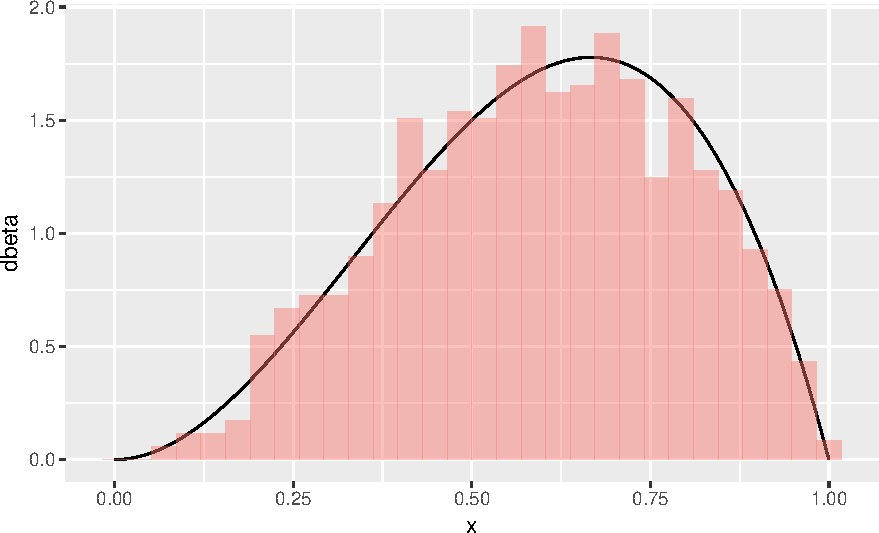
\includegraphics[width=0.7\linewidth]{statistical-computing_files/figure-latex/dbrb-1} 

}

\caption{Beta(3,2) random numbers}\label{fig:dbrb}
\end{figure}

Figure \ref{fig:dbrb} shows that \texttt{rbeta()} function generate random numbers very well. Histogram is of the random number, and the curve is the true beta distribution.

\hypertarget{rvar}{%
\chapter{Methods for Generating Random Variables}\label{rvar}}

\hypertarget{introduction}{%
\section{Introduction}\label{introduction}}

Most of the methods so-called \emph{computational statistics} requires generation of random variables from specified probability distribution. In hand, we can spin wheels, roll a dice, or shuffle cards. The results are chosen randomly. However, we want the same things with computer. Here, \texttt{r}. As we know, computer cannot generate complete uniform random numbers. Instead, we generate \textbf{pseudo-random} numbers.

\hypertarget{pseudo-random-numbers}{%
\section{Pseudo-random Numbers}\label{pseudo-random-numbers}}

\BeginKnitrBlock{definition}[Pseudo-random numbers]
\protect\hypertarget{def:unnamed-chunk-6}{}{\label{def:unnamed-chunk-6} \iffalse (Pseudo-random numbers) \fi{} }Sequence of values generated deterministically which have all the appearances of being independent \(unif(0, 1)\) random variables, i.e.

\[x_1, x_2, \ldots, x_n \stackrel{iid}{\sim} unif(0, 1)\]
\EndKnitrBlock{definition}

\begin{itemize}
\tightlist
\item
  behave \emph{as if} following \(unif(0, 1)\)
\item
  typically generated from an \emph{initial seed}
\end{itemize}

\hypertarget{linear-congruential-generator}{%
\subsection{Linear congruential generator}\label{linear-congruential-generator}}

Then \(u_1, u_2, \ldots, u_n \sim unif(0, 1)\)

\begin{algorithm}[H] \label{alg:alglcg}
  \SetAlgoLined
  \SetKwInOut{Input}{input}
  \SetKwInOut{Output}{output}
  \Input{$a, c \in \mathbb{Z}_{+}$ and modulus $m$}
  Initialize $x_0$\;
  \For{$i \leftarrow 1$ \KwTo $n$}{
    $x_i = (a x_{i - 1} + c) \mod m$\;
  }
  $u_i = \frac{x_i}{m} \in (0, 1)$\;
  \Output{$u_1, u_2, \ldots, u_n \sim unif(0, 1)$}
  \caption{Linear congruential generator}
\end{algorithm}

\begin{Shaded}
\begin{Highlighting}[]
\NormalTok{lcg <-}\StringTok{ }\ControlFlowTok{function}\NormalTok{(n, seed, a, b, m) \{}
\NormalTok{  x <-}\StringTok{ }\KeywordTok{rep}\NormalTok{(seed, n }\OperatorTok{+}\StringTok{ }\DecValTok{1}\NormalTok{)}
  \ControlFlowTok{for}\NormalTok{ (i }\ControlFlowTok{in} \DecValTok{1}\OperatorTok{:}\NormalTok{n) \{}
\NormalTok{    x[i }\OperatorTok{+}\StringTok{ }\DecValTok{1}\NormalTok{] <-}\StringTok{ }\NormalTok{(a }\OperatorTok{*}\StringTok{ }\NormalTok{x[i] }\OperatorTok{+}\StringTok{ }\NormalTok{b) }\OperatorTok\StringTok{ }\NormalTok{m}
\NormalTok{  \}}
\NormalTok{  x[}\OperatorTok{-}\DecValTok{1}\NormalTok{] }\OperatorTok{/}\StringTok{ }\NormalTok{m}
\NormalTok{\}}
\end{Highlighting}
\end{Shaded}

\begin{Shaded}
\begin{Highlighting}[]
\KeywordTok{tibble}\NormalTok{(}
  \DataTypeTok{x =} \KeywordTok{lcg}\NormalTok{(}\DecValTok{1000}\NormalTok{, }\DecValTok{0}\NormalTok{, }\DecValTok{1664525}\NormalTok{, }\DecValTok{1013904223}\NormalTok{, }\DecValTok{2}\OperatorTok{^}\DecValTok{32}\NormalTok{)}
\NormalTok{) }\OperatorTok\StringTok{ }
\StringTok{  }\KeywordTok{ggplot}\NormalTok{(}\KeywordTok{aes}\NormalTok{(}\DataTypeTok{x =}\NormalTok{ x)) }\OperatorTok{+}
\StringTok{  }\KeywordTok{geom_histogram}\NormalTok{(}\KeywordTok{aes}\NormalTok{(}\DataTypeTok{y =}\NormalTok{ ..density..), }\DataTypeTok{bins =} \DecValTok{30}\NormalTok{, }\DataTypeTok{col =} \KeywordTok{gg_hcl}\NormalTok{(}\DecValTok{1}\NormalTok{))}
\end{Highlighting}
\end{Shaded}

\begin{center}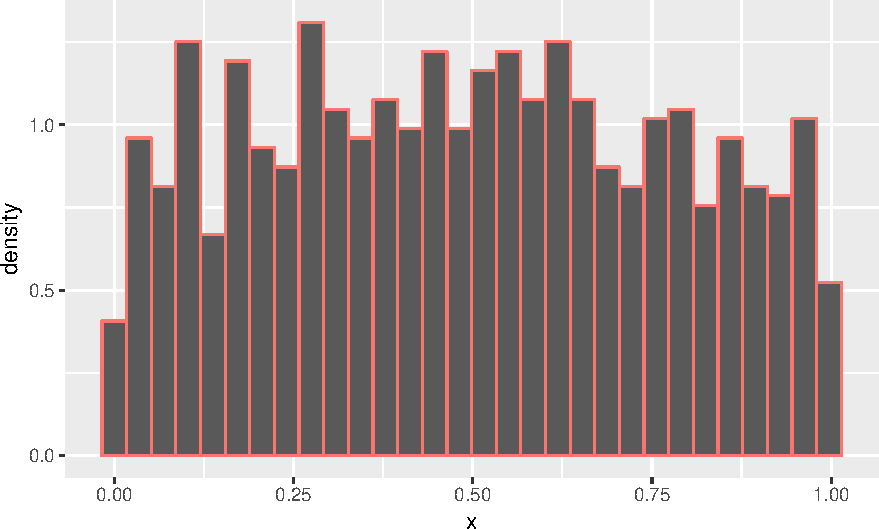
\includegraphics[width=0.7\linewidth]{statistical-computing_files/figure-latex/unnamed-chunk-8-1} \end{center}

\hypertarget{multiplicative-congruential-generator}{%
\subsection{Multiplicative congruential generator}\label{multiplicative-congruential-generator}}

As we can expect from its name, this is congruential generator with \(c = 0\).

\begin{algorithm}[H] \label{alg:algmcg}
  \SetAlgoLined
  \SetKwInOut{Input}{input}
  \SetKwInOut{Output}{output}
  \Input{$a, \in \mathbb{Z}_{+}$ and modulus $m$}
  Initialize $x_0$\;
  \For{$i \leftarrow 1$ \KwTo $n$}{
    $x_i = a x_{i - 1} \mod m$\;
  }
  $u_i = \frac{x_i}{m} \in (0, 1)$\;
  \Output{$u_1, u_2, \ldots, u_n \sim unif(0, 1)$}
  \caption{Multiplicative congruential generator}
\end{algorithm}

We just set \texttt{b\ =\ 0} in our \texttt{lcg()} function. The \textbf{seed must not be zero}.

\begin{Shaded}
\begin{Highlighting}[]
\KeywordTok{tibble}\NormalTok{(}
  \DataTypeTok{x =} \KeywordTok{lcg}\NormalTok{(}\DecValTok{1000}\NormalTok{, }\DecValTok{5}\NormalTok{, }\DecValTok{1664525}\NormalTok{, }\DecValTok{0}\NormalTok{, }\DecValTok{2}\OperatorTok{^}\DecValTok{32}\NormalTok{)}
\NormalTok{) }\OperatorTok\StringTok{ }
\StringTok{  }\KeywordTok{ggplot}\NormalTok{(}\KeywordTok{aes}\NormalTok{(}\DataTypeTok{x =}\NormalTok{ x)) }\OperatorTok{+}
\StringTok{  }\KeywordTok{geom_histogram}\NormalTok{(}\KeywordTok{aes}\NormalTok{(}\DataTypeTok{y =}\NormalTok{ ..density..), }\DataTypeTok{bins =} \DecValTok{30}\NormalTok{, }\DataTypeTok{col =} \KeywordTok{gg_hcl}\NormalTok{(}\DecValTok{1}\NormalTok{))}
\end{Highlighting}
\end{Shaded}

\begin{center}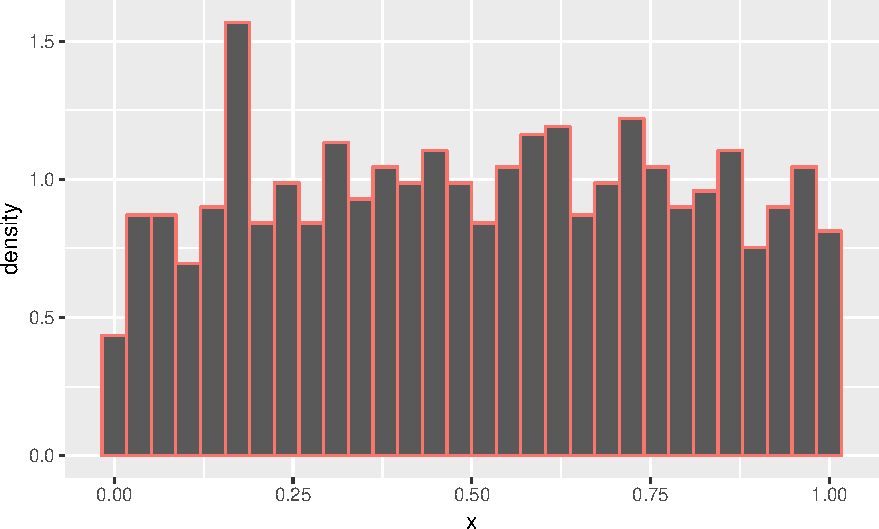
\includegraphics[width=0.7\linewidth]{statistical-computing_files/figure-latex/unnamed-chunk-9-1} \end{center}

\hypertarget{cycle}{%
\subsection{Cycle}\label{cycle}}

Generate LCG \(n = 32\) with \(a = 1\), \(c = 1\), and \(m = 16\) from the seed \(x_0 = 0\).

\begin{Shaded}
\begin{Highlighting}[]
\KeywordTok{lcg}\NormalTok{(}\DecValTok{32}\NormalTok{, }\DecValTok{0}\NormalTok{, }\DecValTok{1}\NormalTok{, }\DecValTok{1}\NormalTok{, }\DecValTok{16}\NormalTok{)}
\CommentTok{#>  [1] 0.0625 0.1250 0.1875 0.2500 0.3125 0.3750 0.4375 0.5000 0.5625 0.6250}
\CommentTok{#> [11] 0.6875 0.7500 0.8125 0.8750 0.9375 0.0000 0.0625 0.1250 0.1875 0.2500}
\CommentTok{#> [21] 0.3125 0.3750 0.4375 0.5000 0.5625 0.6250 0.6875 0.7500 0.8125 0.8750}
\CommentTok{#> [31] 0.9375 0.0000}
\end{Highlighting}
\end{Shaded}

Observe that we have the cycle after \(m\)-th number. Against this problem, we give different seed from every \((im + 1)\)th random number.

\hypertarget{the-inverse-transform-method}{%
\section{The Inverse Transform Method}\label{the-inverse-transform-method}}

\BeginKnitrBlock{definition}[Inverse of CDF]
\protect\hypertarget{def:icdf}{}{\label{def:icdf} \iffalse (Inverse of CDF) \fi{} }Since some cdf \(F_X\) is not strictly increasing, we difine \(F_X^{-1}(y)\) for \(0 < y < 1\) by

\[F_{X}^{-1}(y) := inf \{ x : F_X(x) \ge y \}\]
\EndKnitrBlock{definition}

Using this definition, we can get the following theorem.

\BeginKnitrBlock{theorem}[Probability Integral Transformation]
\protect\hypertarget{thm:probint}{}{\label{thm:probint} \iffalse (Probability Integral Transformation) \fi{} }If \(X\) is a continuous random variable with cdf \(F_(x)\), then
\[U \equiv F_X(X) \sim unif(0, 1)\]
\EndKnitrBlock{theorem}

\BeginKnitrBlock{proof}[Probability Integral Transformation]
\iffalse{} {Proof (Probability Integral Transformation). } \fi{}Let \(U \sim unif(0, 1)\). Then

\begin{equation*}
  \begin{split}
    P(F_X^{-1}(U) \le x) & = P(\inf\{t : F_X(t) = U \} \le x) \\
    & = P(U \le F_X(x)) \\
    & = F_U(F_X(x)) \\
    & = F_X(x)
  \end{split}
\end{equation*}
\EndKnitrBlock{proof}

Thus, to generate \(n\) random variables \(\sim F_X\), we can use \emph{uniform random numbers}.

\begin{algorithm}[H] \label{alg:alginv1}
  \SetAlgoLined
  \SetKwInOut{Input}{input}
  \SetKwInOut{Output}{output}
  \Input{analytical form of $F_X^{-1}$}
  \For{$i \leftarrow 1$ \KwTo $n$}{
    $u_i \stackrel{iid}{\sim}unif(0, 1)$\;
    $x_i = F_X^{-1}(u_i)$\;
  }
  \Output{$x_1, x_2, \ldots, x_n \stackrel{iid}{\sim}F_X$}
  \caption{Inverse transformation method}
\end{algorithm}

Note that in \texttt{R}, vectorized operation would be better, i.e.~generate \texttt{runif(n)} and plug it into given inverse cdf.

\hypertarget{continuous-case}{%
\subsection{Continuous case}\label{continuous-case}}

Denote that the \emph{probability integral transformation} holds for a continuous variable. When generating continuous random variable, applying above algorithm might work.

\BeginKnitrBlock{example}[Exponential distribution]
\protect\hypertarget{exm:expon}{}{\label{exm:expon} \iffalse (Exponential distribution) \fi{} }If \(X \sim Exp(\lambda)\), then \(F_X(x) = 1 - e^{-\lambda x}\). We can derive the inverse function of cdf
\[F_X^{-1}(u) = \frac{1}{\lambda}\ln(1 - u)\]
\EndKnitrBlock{example}

Note that

\[U \sim unif(0, 1) \Leftrightarrow 1 - U \sim unif(0, 1)\]

Then we just can use \(U\) instead of \(1 - U\).

\begin{Shaded}
\begin{Highlighting}[]
\NormalTok{inv_exp <-}\StringTok{ }\ControlFlowTok{function}\NormalTok{(n, lambda) \{}
  \OperatorTok{-}\KeywordTok{log}\NormalTok{(}\KeywordTok{runif}\NormalTok{(n)) }\OperatorTok{/}\StringTok{ }\NormalTok{lambda}
\NormalTok{\}}
\end{Highlighting}
\end{Shaded}

If we generate \(x_1, \ldots, x_{500} \sim Exp(\lambda = 1)\),

\begin{Shaded}
\begin{Highlighting}[]
\KeywordTok{gg_curve}\NormalTok{(dexp, }\DataTypeTok{from =} \DecValTok{0}\NormalTok{, }\DataTypeTok{to =} \DecValTok{10}\NormalTok{) }\OperatorTok{+}
\StringTok{  }\KeywordTok{geom_histogram}\NormalTok{(}
    \DataTypeTok{data =} \KeywordTok{tibble}\NormalTok{(}\DataTypeTok{x =} \KeywordTok{inv_exp}\NormalTok{(}\DecValTok{500}\NormalTok{, }\DataTypeTok{lambda =} \DecValTok{1}\NormalTok{)),}
    \KeywordTok{aes}\NormalTok{(}\DataTypeTok{x =}\NormalTok{ x, }\DataTypeTok{y =}\NormalTok{ ..density..),}
    \DataTypeTok{bins =} \DecValTok{30}\NormalTok{,}
    \DataTypeTok{fill =} \KeywordTok{gg_hcl}\NormalTok{(}\DecValTok{1}\NormalTok{),}
    \DataTypeTok{alpha =} \FloatTok{.5}
\NormalTok{  )}
\end{Highlighting}
\end{Shaded}

\begin{figure}[H]

{\centering 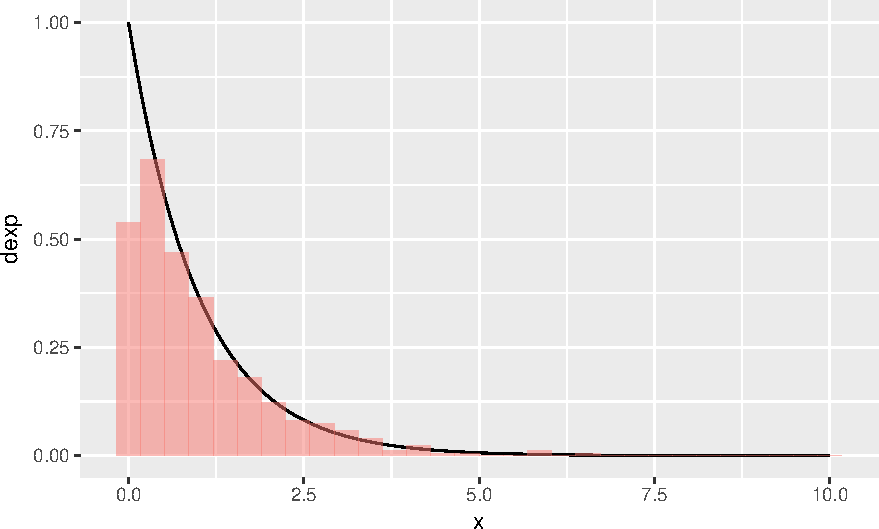
\includegraphics[width=0.7\linewidth]{statistical-computing_files/figure-latex/cdfexp-1} 

}

\caption{Inverse Transformation: Exp(1)}\label{fig:cdfexp}
\end{figure}

\hypertarget{discrete-case}{%
\subsection{Discrete case}\label{discrete-case}}

\begin{algorithm}[H] \label{alg:alginv2}
  \SetAlgoLined
  \SetKwInOut{Input}{input}
  \SetKwInOut{Output}{output}
  \Input{analytical form of $F_X$}
  \For{$i \leftarrow 1$ \KwTo $n$}{
    $u_i \stackrel{iid}{\sim}unif(0, 1)$\;
    Take $x_i$ s.t. $F_X(x_{i - 1}) < U \le F_X(x_i)$\;
  }
  \Output{$x_1, x_2, \ldots, x_n \stackrel{iid}{\sim}F_X$}
  \caption{Inverse transformation method in discrete case}
\end{algorithm}

\begin{longtable}[]{@{}lrrrrr@{}}
\caption{\label{tab:exdis}Example of a Discrete Random Variable}\tabularnewline
\toprule
\endhead
x & 0.0 & 1.0 & 2.0 & 3.0 & 4.0\tabularnewline
p & 0.1 & 0.2 & 0.2 & 0.2 & 0.3\tabularnewline
\bottomrule
\end{longtable}

\BeginKnitrBlock{example}[Discrete Random Variable]
\protect\hypertarget{exm:dismass}{}{\label{exm:dismass} \iffalse (Discrete Random Variable) \fi{} }Consider a discrete random variable \(X\) with a mass function as in Table \ref{tab:exdis}.
\EndKnitrBlock{example}

i.e.

\begin{figure}[H]

{\centering 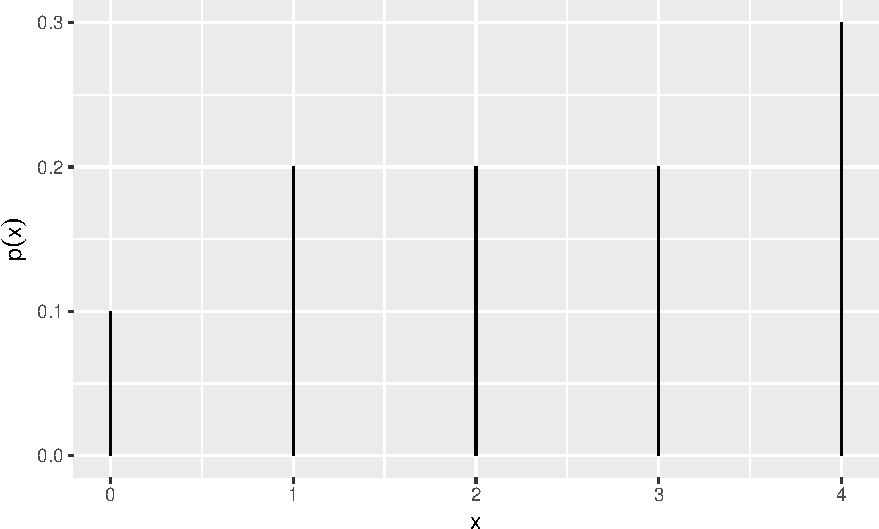
\includegraphics[width=0.7\linewidth]{statistical-computing_files/figure-latex/massfun-1} 

}

\caption{Probability Mass Function}\label{fig:massfun}
\end{figure}

Then we have the cdf

\begin{figure}[H]

{\centering 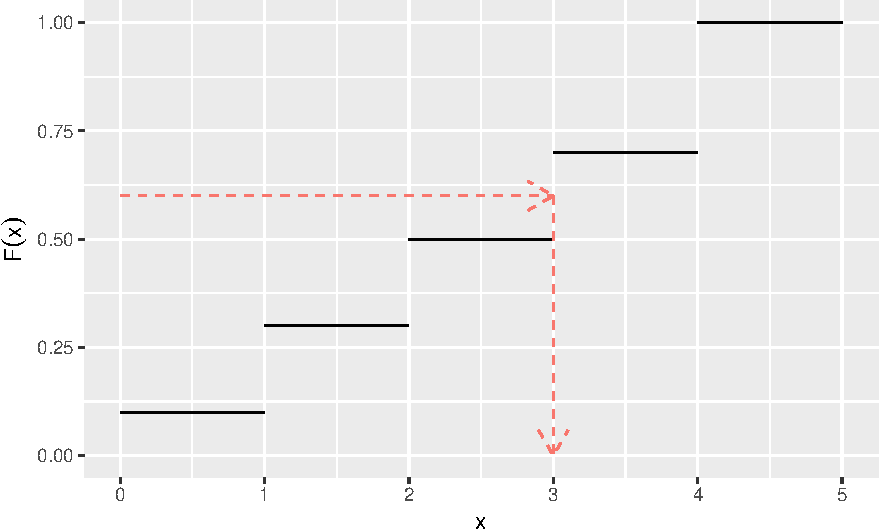
\includegraphics[width=0.7\linewidth]{statistical-computing_files/figure-latex/cdfun-1} 

}

\caption{CDF of the Discrete Random Variable: Illustration for discrete case}\label{fig:cdfun}
\end{figure}

Remembering the algorithm, we can implement \texttt{dplyr::case\_when()} here.

\begin{Shaded}
\begin{Highlighting}[]
\NormalTok{rcustom <-}\StringTok{ }\ControlFlowTok{function}\NormalTok{(n) \{}
  \KeywordTok{tibble}\NormalTok{(}\DataTypeTok{u =} \KeywordTok{runif}\NormalTok{(n)) }\OperatorTok\StringTok{ }
\StringTok{    }\KeywordTok{mutate}\NormalTok{(}
      \DataTypeTok{x =} \KeywordTok{case_when}\NormalTok{(}
\NormalTok{        u }\OperatorTok{>}\StringTok{ }\DecValTok{0} \OperatorTok{&}\StringTok{ }\NormalTok{u }\OperatorTok{<=}\StringTok{ }\FloatTok{.1} \OperatorTok{~}\StringTok{ }\DecValTok{0}\NormalTok{,}
\NormalTok{        u }\OperatorTok{>}\StringTok{ }\FloatTok{.1} \OperatorTok{&}\StringTok{ }\NormalTok{u }\OperatorTok{<=}\StringTok{ }\FloatTok{.3} \OperatorTok{~}\StringTok{ }\DecValTok{1}\NormalTok{,}
\NormalTok{        u }\OperatorTok{>}\StringTok{ }\FloatTok{.3} \OperatorTok{&}\StringTok{ }\NormalTok{u }\OperatorTok{<=}\StringTok{ }\FloatTok{.5} \OperatorTok{~}\StringTok{ }\DecValTok{2}\NormalTok{,}
\NormalTok{        u }\OperatorTok{>}\StringTok{ }\FloatTok{.5} \OperatorTok{&}\StringTok{ }\NormalTok{u }\OperatorTok{<=}\StringTok{ }\FloatTok{.7} \OperatorTok{~}\StringTok{ }\DecValTok{3}\NormalTok{,}
        \OtherTok{TRUE} \OperatorTok{~}\StringTok{ }\DecValTok{4}
\NormalTok{      )}
\NormalTok{    ) }\OperatorTok\StringTok{ }
\StringTok{    }\KeywordTok{select}\NormalTok{(x) }\OperatorTok\StringTok{ }
\StringTok{    }\KeywordTok{pull}\NormalTok{()}
\NormalTok{\}}
\end{Highlighting}
\end{Shaded}

\begin{Shaded}
\begin{Highlighting}[]
\KeywordTok{tibble}\NormalTok{(}\DataTypeTok{x =} \KeywordTok{rcustom}\NormalTok{(}\DecValTok{100}\NormalTok{)) }\OperatorTok\StringTok{ }
\StringTok{  }\KeywordTok{count}\NormalTok{(x) }\OperatorTok\StringTok{ }
\StringTok{  }\KeywordTok{mutate}\NormalTok{(}\DataTypeTok{n =}\NormalTok{ n }\OperatorTok{/}\StringTok{ }\KeywordTok{sum}\NormalTok{(n)) }\OperatorTok\StringTok{ }
\StringTok{  }\KeywordTok{bind_cols}\NormalTok{(}\DataTypeTok{px =}\NormalTok{ pmf }\OperatorTok\StringTok{ }\KeywordTok{select}\NormalTok{(p)) }\OperatorTok\StringTok{ }\CommentTok{# pmf table}
\StringTok{  }\KeywordTok{gather}\NormalTok{(}\OperatorTok{-}\NormalTok{x, }\DataTypeTok{key =} \StringTok{"key"}\NormalTok{, }\DataTypeTok{value =} \StringTok{"value"}\NormalTok{) }\OperatorTok\StringTok{ }
\StringTok{  }\KeywordTok{ggplot}\NormalTok{(}\KeywordTok{aes}\NormalTok{(}\DataTypeTok{x =}\NormalTok{ x, }\DataTypeTok{fill =}\NormalTok{ key)) }\OperatorTok{+}
\StringTok{  }\KeywordTok{geom_bar}\NormalTok{(}\KeywordTok{aes}\NormalTok{(}\DataTypeTok{y =}\NormalTok{ value), }\DataTypeTok{stat =} \StringTok{"identity"}\NormalTok{, }\DataTypeTok{position =} \StringTok{"dodge"}\NormalTok{, }\DataTypeTok{width =} \FloatTok{.2}\NormalTok{) }\OperatorTok{+}
\StringTok{  }\KeywordTok{scale_fill_discrete}\NormalTok{(}
    \DataTypeTok{name =} \StringTok{"Compare"}\NormalTok{,}
    \DataTypeTok{labels =} \KeywordTok{c}\NormalTok{(}\StringTok{"InvTrans"}\NormalTok{, }\KeywordTok{expression}\NormalTok{(}\KeywordTok{p}\NormalTok{(x)))}
\NormalTok{  ) }\OperatorTok{+}
\StringTok{  }\KeywordTok{ylab}\NormalTok{(}\StringTok{"prob"}\NormalTok{)}
\end{Highlighting}
\end{Shaded}

\begin{figure}[H]

{\centering 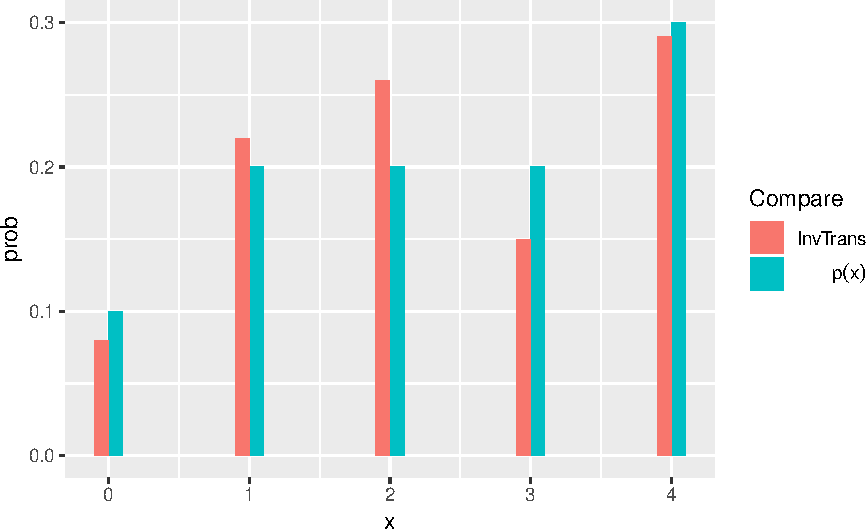
\includegraphics[width=0.7\linewidth]{statistical-computing_files/figure-latex/randmass-1} 

}

\caption{Generated discrete random numbers}\label{fig:randmass}
\end{figure}

See Figure \ref{fig:randmass}. Comparing random numbers to true pmf, the result can be said okay.

\hypertarget{problems-with-inverse-transformation}{%
\subsection{Problems with inverse transformation}\label{problems-with-inverse-transformation}}

Examples \ref{exm:expon} and \ref{exm:dismass}. We could generate these random numbers because we aware of

\begin{enumerate}
\def\labelenumi{\arabic{enumi}.}
\tightlist
\item
  analytical \(F_X\)
\item
  \(F^{-1}\)
\end{enumerate}

In practice, however, not all distribution have analytical \(F\). Numerical computing might be possible, but it is not efficient. There are other approaches.

\hypertarget{the-acceptance-rejection-method}{%
\section{The Acceptance-Rejection Method}\label{the-acceptance-rejection-method}}

Acceptance-rejection method does not require analytical form of cdf. What we need is our \emph{target} density (or mass) function and \emph{proposal} density (or mass) function. Target function is what we want to generate. Propsal function is of any random variable that is \emph{easy to generate random numbers}. From this approach, we can generate any distribution while computation is not efficient.

\begin{longtable}[]{@{}cc@{}}
\toprule
pdf or pmf & target or proposal\tabularnewline
\midrule
\endhead
\(f\) & target\tabularnewline
\(g\) & proposal - easy to generate random numbers\tabularnewline
\bottomrule
\end{longtable}

First of all, \(g\) should satisfy that

\[spt f \subseteq spt g\]

Next, for some (pre-specified) \(c > 0\)

\[\forall x \in spt f : \frac{f(x)}{g(x)} \le c\]

\begin{algorithm}[H] \label{alg:algar}
  \SetAlgoLined
  \SetKwInOut{Input}{input}
  \SetKwInOut{Output}{output}
  \Input{target $f$, proposal $g$, and $c$}
  \For{$i \leftarrow 1$ \KwTo $n$}{
    $Y \sim g(y)$\; \label{alg:argoto}
    $U \sim unif(0, 1) \perp\!\!\!\perp Y$\;
    \eIf{$U \le \frac{f(Y)}{cg(Y)}$}{
      Accept $x_i = Y$\;
    }{
      go to Line \ref{alg:argoto}\;
    }
  }
  \Output{$x_1, x_2, \ldots, x_n \stackrel{iid}{\sim}f(x)$}
  \caption{Acceptance-rejection algorithm}
\end{algorithm}

\hypertarget{efficiency}{%
\subsection{Efficiency}\label{efficiency}}

\begin{figure}[H]

{\centering 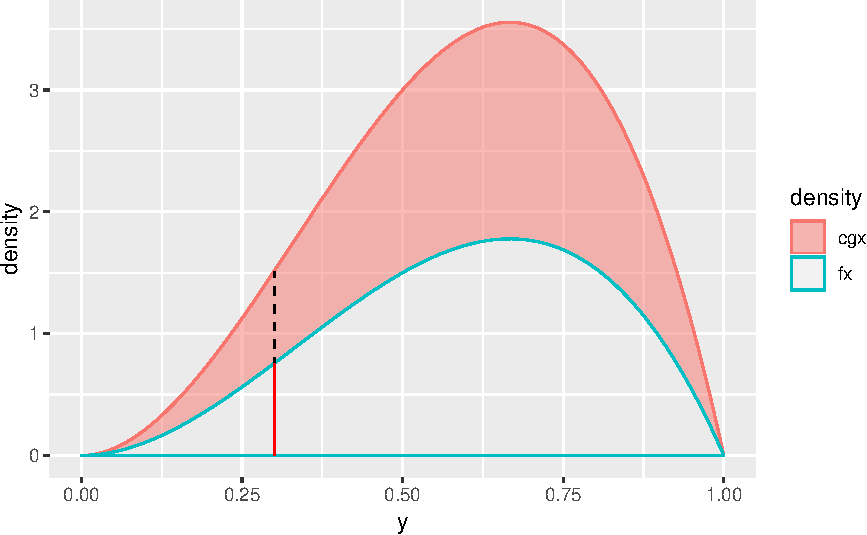
\includegraphics[width=0.7\linewidth]{statistical-computing_files/figure-latex/arprop-1} 

}

\caption{Property of AR method}\label{fig:arprop}
\end{figure}

See Figure \ref{fig:arprop}. This illustrates the motivation of A-R method. Lower one is \(f(x)\) and the upper one is \(cg(x)\) which covers \(f\). We can see that

\[0 < \frac{f(x)}{cg(x)} \le 1\]

The algorithm takes random number from \(Y \sim g\) in each recursive step \(i\), which is represented as a line in the figure. At this value, the algorithm accept \(Y\) as random number of \(f\) if

\[U \le \frac{f(Y)}{cg(Y)}\]

Suppose that we choose a point at random on a line drawn in the figure \ref{fig:arprop}. If we get the red line, we accept. Otherwise, we reject. In other words, the \emph{colored area is where we reject the given value}. The smaller the area is, the more efficient the algorithm will be.

\BeginKnitrBlock{proposition}[Properties of A-R Method]
\protect\hypertarget{prp:arnote}{}{\label{prp:arnote} \iffalse (Properties of A-R Method) \fi{} }See Figure \ref{fig:arprop}.

\begin{enumerate}
  \item $\frac{f(Y)}{cg(Y)} \perp\!\!\!\perp U$
  \item $0 < \frac{f(x)}{cg(x)} \le 1$
  \item Let $N$ be the number of iterations needed to get an acceptance. Then $$N \sim Geo(p) \quad \text{where}\: p \equiv P\bigg(U \le \frac{f(Y)}{cg(Y)}\bigg)$$ and so
$$
\begin{cases}
  P(N = n) = p(1 - p)^{n - 1}I_{\{1, 2, \ldots \}}(n) \\
  E(N) = \text{average number of iterations} = \frac{1}{p}
\end{cases}
$$
  \item $X \sim Y \mid U \le \frac{f(Y)}{cg(Y)}$, i.e. $$P\bigg(Y \le y \mid U \le \frac{f(Y)}{cg(Y)}\bigg) = F_X(y)$$
\end{enumerate}
\EndKnitrBlock{proposition}

\BeginKnitrBlock{remark}[Efficiency]
\iffalse{} {Remark (Efficiency). } \fi{}Efficiency of the A-R method depends on \(p = P\bigg(U \le \frac{f(Y)}{cg(Y)}\bigg)\). In fact,

\[E(N) = \frac{1}{p} = c\]

The algorithm becomes efficient for small \(c\).
\EndKnitrBlock{remark}

\BeginKnitrBlock{proof}
\iffalse{} {Proof. } \fi{}Note that

\[P\bigg( U \le \frac{f(y)}{cg(y)}, Y = y \bigg) = P\bigg(Y \le \frac{g(y)}{cg(y)} \mid Y = y \bigg)P(Y = y)\]

Since \(U \sim unif(0, 1)\), \(P\bigg(Y \le \frac{g(y)}{cg(y)} \mid Y = y \bigg) = \frac{f(y)}{cg(y)}\).

By construction, \(P(Y = y) = g(y)\).

It follows that

\begin{equation*}
  \begin{split}
    p = P\bigg( U \le  \frac{f(y)}{cg(y)} \bigg) & = \int_{-\infty}^{\infty} P\bigg( U \le \frac{f(y)}{cg(y)}, Y = y \bigg) dy \\
    & = \int_{-\infty}^{\infty} \frac{f(y)}{cg(y)} g(y) dy \\
    & = \frac{1}{c} \int_{-\infty}^{\infty}f(y)dy \\
    & = \frac{1}{c}
  \end{split}
\end{equation*}

Hence,

\[E(N) = \frac{1}{p} = c\]

We can say that the method is efficient when the acceptance rate \(p\) is large, i.e.~\(c\) small.
\EndKnitrBlock{proof}

\BeginKnitrBlock{corollary}[Efficiency of A-R Method]
\protect\hypertarget{cor:argood}{}{\label{cor:argood} \iffalse (Efficiency of A-R Method) \fi{} }A-R method is efficient when

\(g(\cdot)\) is close to \(f(\cdot)\) and

have small \(c\).
\EndKnitrBlock{corollary}

\BeginKnitrBlock{corollary}[Choosing c]
\protect\hypertarget{cor:arc}{}{\label{cor:arc} \iffalse (Choosing c) \fi{} }To enhance the algorithm, we might choose \(c\) which satisfy

\[c = \max \bigg\{ \frac{f(x)}{g(x)} : x \in spt f \bigg\}\]
\EndKnitrBlock{corollary}

\hypertarget{examples}{%
\subsection{Examples}\label{examples}}

\BeginKnitrBlock{example}[Beta(a,b)]
\protect\hypertarget{exm:arbeta}{}{\label{exm:arbeta} \iffalse (Beta(a,b)) \fi{} }Let \(X \sim Beta(a, b)\). Then the pdf of \(X\) is given by

\[f(x) = \frac{1}{B(a, b)}x^{a - 1}(1 - x)^{b - 1}I_{(0, 1)}(x)\]
\EndKnitrBlock{example}

\BeginKnitrBlock{solution}[Generating Beta(a,b) with A-R method]
\iffalse{} {Solution (Generating Beta(a,b) with A-R method). } \fi{}Consider proposal density \(g(x) = I_{(0, 1)}(x)\), i.e.~\(unif(0, 1)\).

To determine the optimal \(c\) s.t.

\[c = \max \bigg\{ \frac{f(x)}{g(x)} : x \in (0, 1) \bigg\}\]

find the maximum of

\[\frac{f(x)}{g(x)} = \frac{1}{B(a, b)}x^{a - 1}(1 - x)^{b - 1}\]

Solve

\begin{equation*}
  \begin{split}
    \frac{d}{dx}\bigg(\frac{f(x)}{g(x)}\bigg) & = \frac{1}{B(a, b)}\Big( (a-1)x^{a-2}(1 - x)^{b - 1} - (b - 1)x^{a - 1}(1 - x)^{b - 2} \Big) \\
    & = \frac{x^{a - 2}(1 - x)^{b - 2}}{B(a, b)} \Big( (a - 1)(1 - x) - (b - 1)x \Big) \\
    & = \frac{x^{a - 2}(1 - x)^{b - 2}}{B(a, b)} \big( a - 1 - (a + b - 2)x \big) \quad = 0
  \end{split}
\end{equation*}

It follows that

\[\frac{f(x)}{g(x)} \le \frac{f(\frac{a - 1}{a + b - 2})}{g(\frac{a - 1}{a + b - 2})} = c\]

if \(\frac{a - 1}{a + b - 2} \neq 0, 1\)
\EndKnitrBlock{solution}

\begin{Shaded}
\begin{Highlighting}[]
\NormalTok{ar_beta <-}\StringTok{ }\ControlFlowTok{function}\NormalTok{(n, a, b) \{}
\NormalTok{  opt_x <-}\StringTok{ }\NormalTok{(a }\OperatorTok{-}\StringTok{ }\DecValTok{1}\NormalTok{) }\OperatorTok{/}\StringTok{ }\NormalTok{(a }\OperatorTok{+}\StringTok{ }\NormalTok{b }\OperatorTok{-}\StringTok{ }\DecValTok{2}\NormalTok{)}
\NormalTok{  opt_c <-}\StringTok{ }\KeywordTok{dbeta}\NormalTok{(opt_x, }\DataTypeTok{shape1 =}\NormalTok{ a, }\DataTypeTok{shape2 =}\NormalTok{ b) }\OperatorTok{/}\StringTok{ }\KeywordTok{dunif}\NormalTok{(opt_x)}
\NormalTok{  X <-}\StringTok{ }\OtherTok{NULL}
\NormalTok{  N <-}\StringTok{ }\DecValTok{0}
  \ControlFlowTok{while}\NormalTok{ (N }\OperatorTok{<=}\StringTok{ }\NormalTok{n) \{}
\NormalTok{    Y <-}\StringTok{ }\KeywordTok{runif}\NormalTok{(n)}
\NormalTok{    U <-}\StringTok{ }\KeywordTok{runif}\NormalTok{(n)}
\NormalTok{    X <-}\StringTok{ }\KeywordTok{c}\NormalTok{(X, Y[U }\OperatorTok{<=}\StringTok{ }\KeywordTok{dbeta}\NormalTok{(Y, }\DataTypeTok{shape1 =}\NormalTok{ a, }\DataTypeTok{shape2 =}\NormalTok{ b) }\OperatorTok{/}\StringTok{ }\NormalTok{opt_c])}
\NormalTok{    N <-}\StringTok{ }\KeywordTok{length}\NormalTok{(X)}
    \ControlFlowTok{if}\NormalTok{ ( N }\OperatorTok{>}\StringTok{ }\NormalTok{n ) X <-}\StringTok{ }\NormalTok{X[}\DecValTok{1}\OperatorTok{:}\NormalTok{n]}
\NormalTok{  \}}
\NormalTok{  X}
\NormalTok{\}}
\end{Highlighting}
\end{Shaded}

Now we try to compare this A-R function to \texttt{R} \texttt{rbeta} function.

\begin{Shaded}
\begin{Highlighting}[]
\NormalTok{gen_beta <-}
\StringTok{  }\KeywordTok{tibble}\NormalTok{(}
    \DataTypeTok{ar_rand =} \KeywordTok{ar_beta}\NormalTok{(}\DecValTok{1000}\NormalTok{, }\DecValTok{3}\NormalTok{, }\DecValTok{2}\NormalTok{),}
    \DataTypeTok{sam =} \KeywordTok{rbeta}\NormalTok{(}\DecValTok{1000}\NormalTok{, }\DecValTok{3}\NormalTok{, }\DecValTok{2}\NormalTok{)}
\NormalTok{  ) }\OperatorTok\StringTok{ }
\StringTok{  }\KeywordTok{gather}\NormalTok{(}\DataTypeTok{key =} \StringTok{"den"}\NormalTok{, }\DataTypeTok{value =} \StringTok{"value"}\NormalTok{)}
\end{Highlighting}
\end{Shaded}

\begin{Shaded}
\begin{Highlighting}[]
\KeywordTok{gg_curve}\NormalTok{(dbeta, }\DataTypeTok{from =} \DecValTok{0}\NormalTok{, }\DataTypeTok{to =} \DecValTok{1}\NormalTok{, }\DataTypeTok{args =} \KeywordTok{list}\NormalTok{(}\DataTypeTok{shape1 =} \DecValTok{3}\NormalTok{, }\DataTypeTok{shape2 =} \DecValTok{2}\NormalTok{)) }\OperatorTok{+}
\StringTok{  }\KeywordTok{geom_histogram}\NormalTok{(}
    \DataTypeTok{data =}\NormalTok{ gen_beta,}
    \KeywordTok{aes}\NormalTok{(}\DataTypeTok{x =}\NormalTok{ value, }\DataTypeTok{y =}\NormalTok{ ..density.., }\DataTypeTok{fill =}\NormalTok{ den),}
    \DataTypeTok{position =} \StringTok{"identity"}\NormalTok{,}
    \DataTypeTok{bins =} \DecValTok{30}\NormalTok{,}
    \DataTypeTok{alpha =} \FloatTok{.45}
\NormalTok{  ) }\OperatorTok{+}
\StringTok{  }\KeywordTok{scale_fill_discrete}\NormalTok{(}
    \DataTypeTok{name =} \StringTok{"random number"}\NormalTok{,}
    \DataTypeTok{labels =} \KeywordTok{c}\NormalTok{(}\StringTok{"AR"}\NormalTok{, }\StringTok{"rbeta"}\NormalTok{)}
\NormalTok{  )}
\end{Highlighting}
\end{Shaded}

\begin{figure}[H]

{\centering 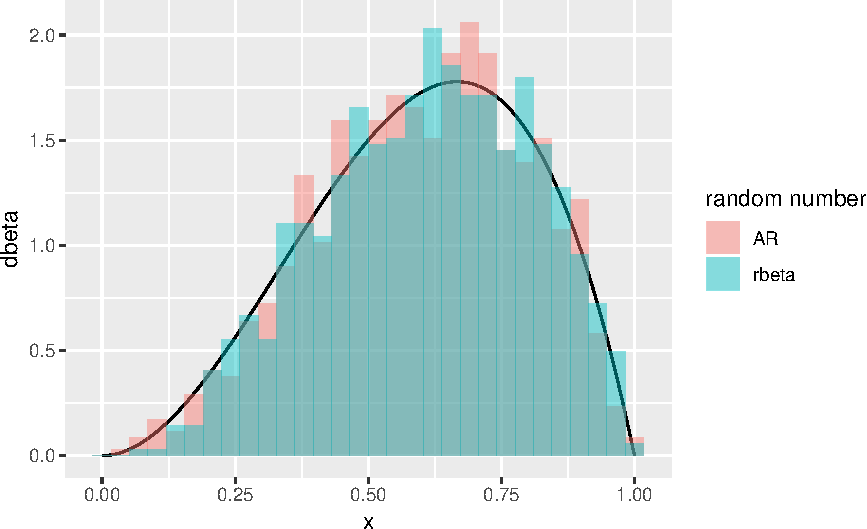
\includegraphics[width=0.7\linewidth]{statistical-computing_files/figure-latex/betahis-1} 

}

\caption{Beta(3,2) Random numbers from each function}\label{fig:betahis}
\end{figure}

In the Figure \ref{fig:betahis}, the both histograms are very close to the true density curve. To see more statistically, we can draw a Q-Q plot.

\begin{Shaded}
\begin{Highlighting}[]
\NormalTok{gen_beta }\OperatorTok\StringTok{ }
\StringTok{  }\KeywordTok{ggplot}\NormalTok{(}\KeywordTok{aes}\NormalTok{(}\DataTypeTok{sample =}\NormalTok{ value)) }\OperatorTok{+}
\StringTok{  }\KeywordTok{stat_qq_line}\NormalTok{(}
    \DataTypeTok{distribution =}\NormalTok{ stats}\OperatorTok{::}\NormalTok{qbeta,}
    \DataTypeTok{dparams =} \KeywordTok{list}\NormalTok{(}\DataTypeTok{shape1 =} \DecValTok{3}\NormalTok{, }\DataTypeTok{shape2 =} \DecValTok{2}\NormalTok{),}
    \DataTypeTok{col =} \KeywordTok{I}\NormalTok{(}\StringTok{"grey70"}\NormalTok{),}
    \DataTypeTok{size =} \FloatTok{3.5}
\NormalTok{  ) }\OperatorTok{+}
\StringTok{  }\KeywordTok{stat_qq}\NormalTok{(}
    \KeywordTok{aes}\NormalTok{(}\DataTypeTok{colour =}\NormalTok{ den),}
    \DataTypeTok{distribution =}\NormalTok{ stats}\OperatorTok{::}\NormalTok{qbeta,}
    \DataTypeTok{dparams =} \KeywordTok{list}\NormalTok{(}\DataTypeTok{shape1 =} \DecValTok{3}\NormalTok{, }\DataTypeTok{shape2 =} \DecValTok{2}\NormalTok{)}
\NormalTok{  ) }\OperatorTok{+}
\StringTok{  }\KeywordTok{scale_colour_discrete}\NormalTok{(}
    \DataTypeTok{name =} \StringTok{"random number"}\NormalTok{,}
    \DataTypeTok{labels =} \KeywordTok{c}\NormalTok{(}\StringTok{"AR"}\NormalTok{, }\StringTok{"rbeta"}\NormalTok{)}
\NormalTok{  )}
\end{Highlighting}
\end{Shaded}

\begin{figure}[H]

{\centering 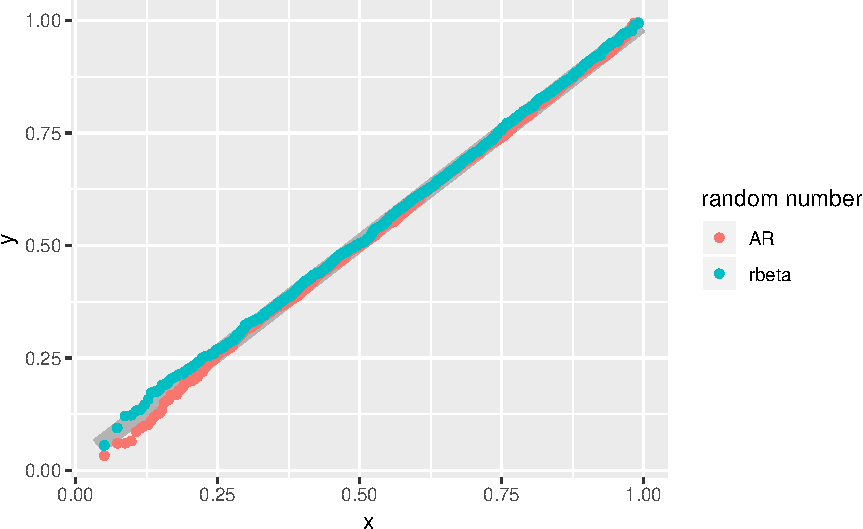
\includegraphics[width=0.7\linewidth]{statistical-computing_files/figure-latex/betaqq-1} 

}

\caption{Q-Q plot for Beta(3,2) random numbers}\label{fig:betaqq}
\end{figure}

See Figure \ref{fig:betaqq}. We have got series of numbers that are sticked to the beta distribution line.

\BeginKnitrBlock{example}[A-R Method for Discrete case]
\protect\hypertarget{exm:ardiscrete}{}{\label{exm:ardiscrete} \iffalse (A-R Method for Discrete case) \fi{} }A-R method can be also implemented to discrete case such as Example \ref{exm:dismass}.
\EndKnitrBlock{example}

\begin{longtable}[]{@{}lrrrrr@{}}
\caption{\label{tab:exdis2}Example of a Discrete Random Variable}\tabularnewline
\toprule
\endhead
x & 0.0 & 1.0 & 2.0 & 3.0 & 4.0\tabularnewline
p & 0.1 & 0.2 & 0.2 & 0.2 & 0.3\tabularnewline
\bottomrule
\end{longtable}

\BeginKnitrBlock{solution}[Generating discrete random numbers using A-R methods]
\iffalse{} {Solution (Generating discrete random numbers using A-R methods). } \fi{}Consider proposal \(g(x) \sim \text{Discrete unif}(0, 1, 2, 3, 4)\), i.e.

\[g(0) = g(1) = \cdots = g(4) = 0.2\]

Then we set

\[c = \max\bigg\{ \frac{p(x)}{g(x)} : x = 0, \ldots, 4 \bigg\} = \max\Big\{ 0.5, 1, 1.5 \Big\} = 1.5\]
\EndKnitrBlock{solution}

\hypertarget{transfomation-methods}{%
\section{Transfomation Methods}\label{transfomation-methods}}

\hypertarget{continuous}{%
\subsection{Continuous}\label{continuous}}

\BeginKnitrBlock{proposition}[Transformation between continuous random variables]
\protect\hypertarget{prp:trans1}{}{\label{prp:trans1} \iffalse (Transformation between continuous random variables) \fi{} }Relation between random variables enables generating target numbers from the others.

\begin{enumerate}
  \item $Z_1, \ldots, Z_n \stackrel{iid}{\sim}N(0, 1) \Rightarrow \sum Z_i^2 \sim \chi^2(n)$
  \item $Y_1 \sim \chi^2(m) \perp\!\!\!\perp Y_2 \sim \chi^2(n) \Rightarrow \frac{Y_1 / m}{Y_2 / n} \sim F(m, n)$
  \item $Z \sim N(0, 1) \perp\!\!\!\perp Y \sim \chi^2(n) \Rightarrow \frac{Z}{\sqrt{Y / n}} \sim t(n)$
  \item $Y_1, \ldots, Y_n \stackrel{iid}{\sim}Exp(\lambda) \Rightarrow \sum Y_i^2 Gamma(n, \lambda)$
  \item $U \sim unif(0, 1) \Rightarrow (b - a)U + a \sim unif(a, b)$
  \item $U \sim Gamma(r, \lambda) \perp\!\!\!\perp V \sim Gamma(s, \lambda) \Rightarrow \frac{U}{U + V} \sim Beta(r, s)$
  \item $Z \sim N(0, 1) \Rightarrow \mu + \sigma Z \sim N(\mu, \sigma^2)$
  \item $Y \sim N(\mu, \sigma^2) \Rightarrow e^Y \sim LogNormal(\mu, \sigma^2)$
\end{enumerate}
\EndKnitrBlock{proposition}

\BeginKnitrBlock{example}[Generating Beta(a, b) using rgamma]
\protect\hypertarget{exm:transbeta}{}{\label{exm:transbeta} \iffalse (Generating Beta(a, b) using rgamma) \fi{} }From Proposition \ref{prp:trans1}, we can generate \(Beta(a,b)\) random numbers using \(Gamma(a, 1)\) and \(Gamma(b, 1)\).
\EndKnitrBlock{example}

\begin{Shaded}
\begin{Highlighting}[]
\NormalTok{trans_beta <-}\StringTok{ }\ControlFlowTok{function}\NormalTok{(n, shape1, shape2) \{}
\NormalTok{  u <-}\StringTok{ }\KeywordTok{rgamma}\NormalTok{(n, }\DataTypeTok{shape =}\NormalTok{ shape1, }\DataTypeTok{rate =} \DecValTok{1}\NormalTok{)}
\NormalTok{  v <-}\StringTok{ }\KeywordTok{rgamma}\NormalTok{(n, }\DataTypeTok{shape =}\NormalTok{ shape2, }\DataTypeTok{rate =} \DecValTok{1}\NormalTok{)}
\NormalTok{  u }\OperatorTok{/}\StringTok{ }\NormalTok{(u }\OperatorTok{+}\StringTok{ }\NormalTok{v)}
\NormalTok{\}}
\end{Highlighting}
\end{Shaded}

\begin{figure}[H]

{\centering 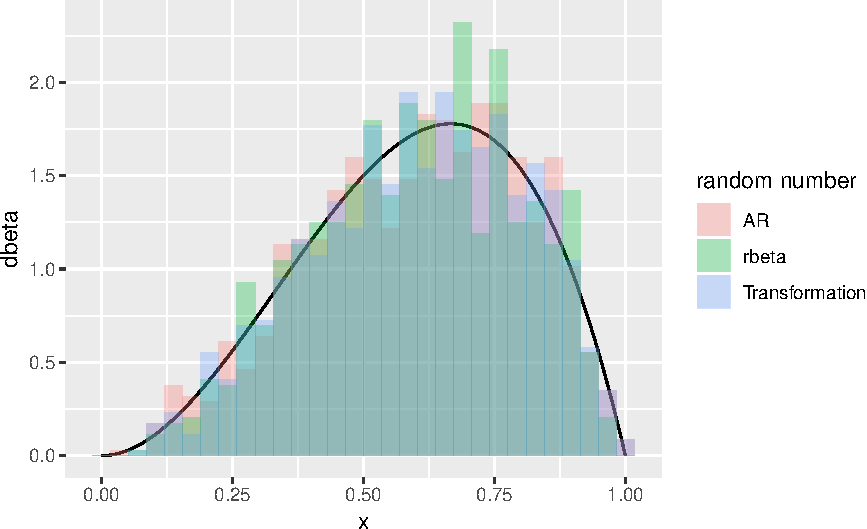
\includegraphics[width=0.7\linewidth]{statistical-computing_files/figure-latex/tbetafig-1} 

}

\caption{Beta(3,2) Random numbers from each function, including transformation method}\label{fig:tbetafig}
\end{figure}

\hypertarget{box-muller-transformation}{%
\subsection{Box-Muller transformation}\label{box-muller-transformation}}

Denote that Gaussian cdf has no closed form of \(F_X^{-1}\). Using polar coordiantes, we can generate Normal random numers.

\BeginKnitrBlock{theorem}[Box-Muller transformation]
\protect\hypertarget{thm:bmnorm}{}{\label{thm:bmnorm} \iffalse (Box-Muller transformation) \fi{} }Let \(U_1, U_2 \stackrel{iid}{\sim}unif(0,1)\). Then

\[
\begin{cases}
  Z_1 = \sqrt{-2 \ln U_2} \cos(2\pi U_1) \\
  Z_2 = \sqrt{-2 \ln U_2} \sin(2\pi U_1)
\end{cases}
\]
\EndKnitrBlock{theorem}

\BeginKnitrBlock{proof}
\iffalse{} {Proof. } \fi{}Write

\[
(Z_1, Z_2)^T \sim N\bigg( \begin{bmatrix}
  0 \\
  0
\end{bmatrix}, \begin{bmatrix}
  1 & 0 \\
  0 & 1
\end{bmatrix} \bigg)
\]

Then the joint pdf is given by

\[f_{Z_1, Z_2}(x_1, x_2) = \frac{1}{2\pi}\exp\bigg(-\frac{x_1^2 + x_2^2}{2}\bigg)\]

Consider polar coordiate transformation \((R, \theta)\): \(x_1 = R\cos\theta\) and \(x_2 = R\sin\theta\).

Since it is also random vector,

\begin{equation*}
  \begin{split}
    f_{R, \theta}(r, \theta) & = f_{Z_1, Z_2}(x_1, x_2)\lvert J \rvert \\
    & = \frac{1}{2\pi}\exp\bigg(-\frac{x_1^2 + x_2^2}{2}\bigg)\left\lvert\begin{array}{cc}
      \frac{\partial x_1}{\partial r} & \frac{\partial x_1}{\partial \theta} \\
      \frac{\partial x_2}{\partial r} & \frac{\partial x_2}{\partial \theta}
    \end{array}\right\rvert \\
    & = \frac{1}{2\pi}\exp\bigg(-\frac{r^2}{2}\bigg)\left\lvert\begin{array}{cc}
      \frac{\partial x_1}{\partial r} & \frac{\partial x_1}{\partial \theta} \\
      \frac{\partial x_2}{\partial r} & \frac{\partial x_2}{\partial \theta}
    \end{array}\right\rvert \\
    & = \frac{r}{2\pi}\exp\bigg(-\frac{r^2}{2}\bigg)
  \end{split}
\end{equation*}

Then each marginal density function can be computed as

\begin{equation*}
  \begin{split}
    f_{\theta}(\theta) & = \int_0^\infty \frac{r}{2\pi}\exp\bigg(-\frac{r^2}{2}\bigg) dr \\
    & = \frac{1}{2\pi} I_{(0, 2\pi)}(\theta) \\
    & \stackrel{d}{=} unif(0, 2\pi)
  \end{split}
\end{equation*}

\begin{equation*}
  \begin{split}
    f_R(r) & = \int_0^\theta \frac{r}{2\pi}\exp\bigg(-\frac{r^2}{2}\bigg) d\theta \\
    & = r \exp\bigg(-\frac{r^2}{2}\bigg) I_{(0, \infty)}(r)
  \end{split}
\end{equation*}

Thus,

\[f_{R,\theta} = f_{\theta}f_R \Rightarrow R \perp\!\!\!\perp\theta\]

It follows from inverse transformation theorem that

\[Z_1 = R\cos\theta = \sqrt{-2 \ln U_2} \cos(2\pi U_1)\]

and that

\[Z_2 = R\sin\theta = \sqrt{-2 \ln U_2} \sin(2\pi U_1)\]

where \(U_1, U_2 \stackrel{iid}{\sim}unif(0, 1)\)
\EndKnitrBlock{proof}

\begin{algorithm}[H] \label{alg:algbm}
  \SetAlgoLined
  \SetKwInOut{Input}{input}
  \SetKwInOut{Output}{output}
  \For{$i \leftarrow 1$ \KwTo $n$}{
    $U_1, U_2 \stackrel{iid}{\sim}unif(0,1)$\;
    $z_{2i - 1} = \sqrt{-2\ln U_2}\cos(2\pi U_1)$\;
    $z_{2i} = \sqrt{-2\ln U_2}\sin(2\pi U_1)$\;
  }
  \Output{$z_1, \ldots, z_n \stackrel{iid}{\sim}N(0,1)$}
  \caption{Box-Muller transformation}
\end{algorithm}

\begin{Shaded}
\begin{Highlighting}[]
\NormalTok{bmnorm <-}\StringTok{ }\ControlFlowTok{function}\NormalTok{(n, }\DataTypeTok{mean =} \DecValTok{0}\NormalTok{, }\DataTypeTok{sd =} \DecValTok{1}\NormalTok{) \{}
\NormalTok{  n_bm <-}\StringTok{ }\KeywordTok{ceiling}\NormalTok{(n }\OperatorTok{/}\StringTok{ }\DecValTok{2}\NormalTok{)}
  \KeywordTok{tibble}\NormalTok{(}
    \DataTypeTok{theta =} \KeywordTok{runif}\NormalTok{(}\DataTypeTok{n =}\NormalTok{ n_bm, }\DataTypeTok{max =} \DecValTok{2} \OperatorTok{*}\StringTok{ }\NormalTok{pi),}
    \DataTypeTok{R =} \KeywordTok{sqrt}\NormalTok{(}\OperatorTok{-}\DecValTok{2} \OperatorTok{*}\StringTok{ }\KeywordTok{log}\NormalTok{(}\KeywordTok{runif}\NormalTok{(n_bm)))}
\NormalTok{  ) }\OperatorTok\StringTok{ }
\StringTok{    }\KeywordTok{mutate}\NormalTok{(}
      \DataTypeTok{x1 =}\NormalTok{ R }\OperatorTok{*}\StringTok{ }\KeywordTok{cos}\NormalTok{(theta),}
      \DataTypeTok{x2 =}\NormalTok{ R }\OperatorTok{*}\StringTok{ }\KeywordTok{sin}\NormalTok{(theta)}
\NormalTok{    ) }\OperatorTok\StringTok{ }
\StringTok{    }\KeywordTok{gather}\NormalTok{(x1, x2, }\DataTypeTok{key =} \StringTok{"key"}\NormalTok{, }\DataTypeTok{value =} \StringTok{"value"}\NormalTok{) }\OperatorTok\StringTok{ }
\StringTok{    }\KeywordTok{mutate}\NormalTok{(}\DataTypeTok{value =}\NormalTok{ mean }\OperatorTok{+}\StringTok{ }\NormalTok{sd }\OperatorTok{*}\StringTok{ }\NormalTok{value) }\OperatorTok\StringTok{ }
\StringTok{    }\KeywordTok{select}\NormalTok{(value) }\OperatorTok\StringTok{ }
\StringTok{    }\KeywordTok{pull}\NormalTok{()}
\NormalTok{\}}
\end{Highlighting}
\end{Shaded}

\begin{Shaded}
\begin{Highlighting}[]
\KeywordTok{gg_curve}\NormalTok{(dnorm, }\DataTypeTok{from =} \DecValTok{0}\NormalTok{, }\DataTypeTok{to =} \DecValTok{6}\NormalTok{, }\DataTypeTok{args =} \KeywordTok{list}\NormalTok{(}\DataTypeTok{mean =} \DecValTok{3}\NormalTok{, }\DataTypeTok{sd =} \DecValTok{1}\NormalTok{)) }\OperatorTok{+}
\StringTok{  }\KeywordTok{geom_histogram}\NormalTok{(}
    \DataTypeTok{data =} \KeywordTok{tibble}\NormalTok{(}\DataTypeTok{x =} \KeywordTok{bmnorm}\NormalTok{(}\DecValTok{1000}\NormalTok{, }\DataTypeTok{mean =} \DecValTok{3}\NormalTok{, }\DataTypeTok{sd =} \DecValTok{1}\NormalTok{)),}
    \KeywordTok{aes}\NormalTok{(}\DataTypeTok{x =}\NormalTok{ x, }\DataTypeTok{y =}\NormalTok{ ..density..),}
    \DataTypeTok{bins =} \DecValTok{30}\NormalTok{,}
    \DataTypeTok{fill =} \KeywordTok{gg_hcl}\NormalTok{(}\DecValTok{1}\NormalTok{),}
    \DataTypeTok{alpha =} \FloatTok{.5}
\NormalTok{  )}
\end{Highlighting}
\end{Shaded}

\begin{figure}[H]

{\centering 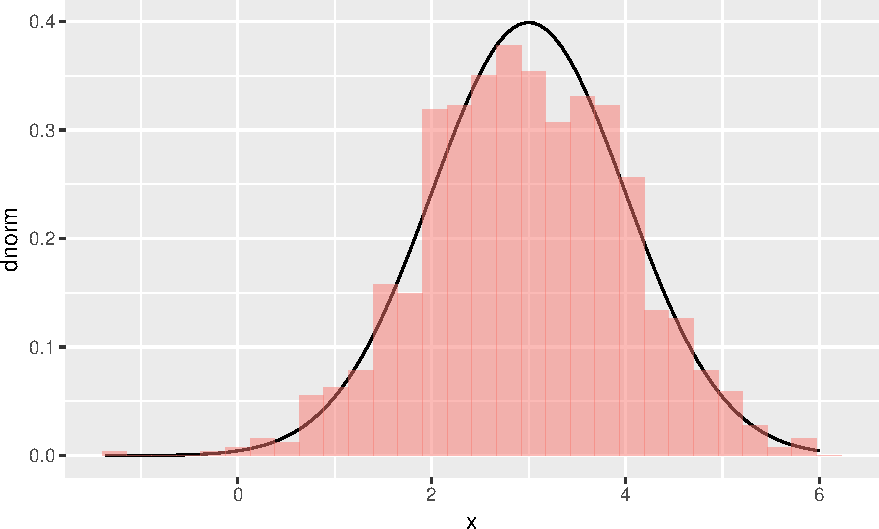
\includegraphics[width=0.7\linewidth]{statistical-computing_files/figure-latex/boxnorm-1} 

}

\caption{Normal random numbers by Box-Muller transformation}\label{fig:boxnorm}
\end{figure}

\hypertarget{discrete}{%
\subsection{Discrete}\label{discrete}}

\BeginKnitrBlock{proposition}[Transformation between discrete random variables]
\protect\hypertarget{prp:trans2}{}{\label{prp:trans2} \iffalse (Transformation between discrete random variables) \fi{} }Relation between random variables enables generating target numbers from the others.

\begin{enumerate}
  \item $Y_1, \ldots, Y_n \stackrel{iid}{\sim}Bernoulli(p) \Rightarrow \sum Y_i^2 \sim B(n, p)$
  \item $U \sim unif(0,1) \Rightarrow X_i = \lfloor mU \rfloor + 1$
  \item $X = \text{the number of events occurring in 1 unit of time} \sim Poisson(\lambda)$
\end{enumerate}
\EndKnitrBlock{proposition}

\BeginKnitrBlock{proposition}[Bernoulli process]
\protect\hypertarget{prp:trans3}{}{\label{prp:trans3} \iffalse (Bernoulli process) \fi{} }Let \(X_1, X_2, \ldots \stackrel{iid}{\sim}Bernoulli(p)\).

\begin{enumerate}
  \item $N = \text{the number of trials until we see a success, i.e.} X_N = 1 \Rightarrow N \sim Geo(p)$
  \item $Y_1, \ldots, Y_r \stackrel{iid}{\sim}Geo(p) \Rightarrow \sum\limits_{i = 1}^r Y_i = \text{the number of trials until we see r successes} \sim NegBin(r, p)$
\end{enumerate}
\EndKnitrBlock{proposition}

\BeginKnitrBlock{proposition}[Count process]
\protect\hypertarget{prp:trans4}{}{\label{prp:trans4} \iffalse (Count process) \fi{} }Let \(Y_1, Y_2, \ldots \stackrel{iid}{\sim}Exp(\lambda)\) be interarrival times. Then

\[X = \max\{ n : \sum Y_i \le 1 \} = \text{the number of events occurring in 1 unit of time} \sim Poisson(\lambda)\]
\EndKnitrBlock{proposition}

\hypertarget{sums-and-mixtures}{%
\section{Sums and Mixtures}\label{sums-and-mixtures}}

\hypertarget{convolutions}{%
\subsection{Convolutions}\label{convolutions}}

\BeginKnitrBlock{definition}[Convolution]
\protect\hypertarget{def:conv}{}{\label{def:conv} \iffalse (Convolution) \fi{} }Let \(X_1, \ldots, X_n\) be independent and identically distributed and let \(S = X_1 + \cdots X_n\). Then the distribution of \(S\) is called the \(n\)-fold convolution of \(X\) and denoted by \(F_X^{*(n)}\).
\EndKnitrBlock{definition}

In the last chapter, we have already seen a bunch of random variables that can be generated by summing the other.

\BeginKnitrBlock{example}[Chisquare]
\protect\hypertarget{exm:rchi}{}{\label{exm:rchi} \iffalse (Chisquare) \fi{} }Let \(Z_1, \ldots, Z_n \stackrel{iid}{\sim}N(0, 1)\). We know from Proposition \ref{prp:trans1} that

\[V = \sum_{i = 1}^n Z_i \sim \chi^2(n)\]
\EndKnitrBlock{example}

Building a \texttt{n} \(\times\) \texttt{df} matrix can be a good strategy here. After that, \texttt{rowSums} or \texttt{colSums} ends the generation work.

\begin{Shaded}
\begin{Highlighting}[]
\NormalTok{conv_chisq <-}\StringTok{ }\ControlFlowTok{function}\NormalTok{(n, df) \{}
\NormalTok{  X <-}
\StringTok{    }\KeywordTok{matrix}\NormalTok{(}\KeywordTok{rnorm}\NormalTok{(n }\OperatorTok{*}\StringTok{ }\NormalTok{df), }\DataTypeTok{nrow =}\NormalTok{ n, }\DataTypeTok{ncol =}\NormalTok{ df)}\OperatorTok{^}\DecValTok{2}
  \KeywordTok{rowSums}\NormalTok{(X)}
\NormalTok{\}}
\end{Highlighting}
\end{Shaded}

\begin{Shaded}
\begin{Highlighting}[]
\KeywordTok{gg_curve}\NormalTok{(dchisq, }\DataTypeTok{from =} \DecValTok{0}\NormalTok{, }\DataTypeTok{to =} \DecValTok{15}\NormalTok{, }\DataTypeTok{args =} \KeywordTok{list}\NormalTok{(}\DataTypeTok{df =} \DecValTok{5}\NormalTok{)) }\OperatorTok{+}
\StringTok{  }\KeywordTok{geom_histogram}\NormalTok{(}
    \DataTypeTok{data =} \KeywordTok{tibble}\NormalTok{(}\DataTypeTok{x =} \KeywordTok{conv_chisq}\NormalTok{(}\DecValTok{1000}\NormalTok{, }\DataTypeTok{df =} \DecValTok{5}\NormalTok{)),}
    \KeywordTok{aes}\NormalTok{(}\DataTypeTok{x =}\NormalTok{ x, }\DataTypeTok{y =}\NormalTok{ ..density..),}
    \DataTypeTok{bins =} \DecValTok{30}\NormalTok{,}
    \DataTypeTok{fill =} \KeywordTok{gg_hcl}\NormalTok{(}\DecValTok{1}\NormalTok{),}
    \DataTypeTok{alpha =} \FloatTok{.5}
\NormalTok{  )}
\end{Highlighting}
\end{Shaded}

\begin{figure}[H]

{\centering 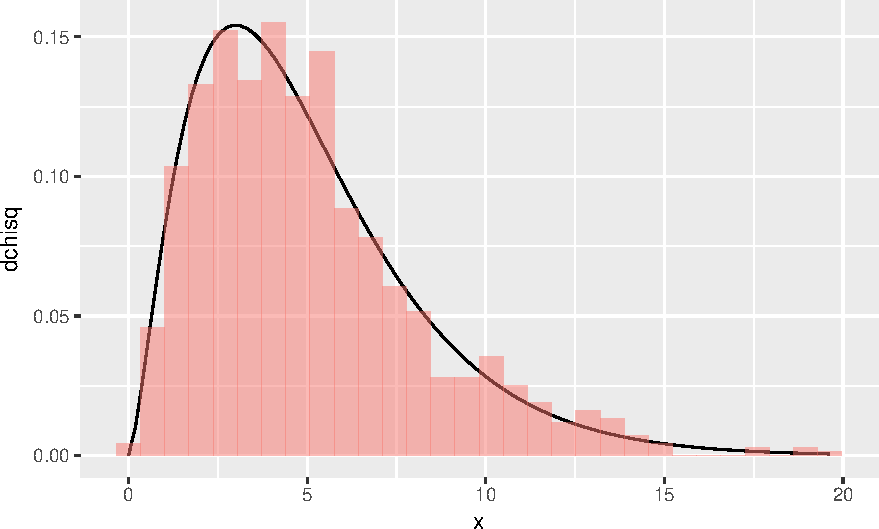
\includegraphics[width=0.7\linewidth]{statistical-computing_files/figure-latex/convchi-1} 

}

\caption{$\chi^2$ random numbers from Normal sums}\label{fig:convchi}
\end{figure}

\hypertarget{mixtures}{%
\subsection{Mixtures}\label{mixtures}}

\BeginKnitrBlock{definition}[Discrete mixture]
\protect\hypertarget{def:mixprob1}{}{\label{def:mixprob1} \iffalse (Discrete mixture) \fi{} }A random variable \(X\) is a discrete mixture if the distribution of \(X\) is a weighted sum

\[F_X(x) = \sum \theta_i F_{X_i}(x)\]

where constants \(\theta_i\) are called the mixing weights or mixing probabilities.
\EndKnitrBlock{definition}

\BeginKnitrBlock{definition}[Continuous mixture]
\protect\hypertarget{def:mixprob2}{}{\label{def:mixprob2} \iffalse (Continuous mixture) \fi{} }A random variable \(X\) is a continuous mixture if the distribution of \(X\) is a weighted sum

\[F_X(x) = \int_\infty^\infty F_{X \mid Y = y} (x) f_Y(y) dy\]
\EndKnitrBlock{definition}

\BeginKnitrBlock{example}[Mixture of several Normal distributions]
\protect\hypertarget{exm:gaussmix}{}{\label{exm:gaussmix} \iffalse (Mixture of several Normal distributions) \fi{} }Generate a random sample of size \(1000\) from a normal location mixture with components of the mixture \(N(0,1)\) and \(N(3,1)\), i.e.

\[F_X = p_1 F_{X_1} + (1 - p_1) F_{X_2}\]
\EndKnitrBlock{example}

To combine samples easily, we use \texttt{foreach} library.

\begin{Shaded}
\begin{Highlighting}[]
\KeywordTok{library}\NormalTok{(foreach)}
\end{Highlighting}
\end{Shaded}

As in A-R method, Bernoullin splitting would be used.

\[
\begin{cases}
  F_{X_1} & U > p_1 \\
  F_{X_2} & \text{otherwise}
\end{cases}
\]

\begin{Shaded}
\begin{Highlighting}[]
\NormalTok{mix_norm <-}\StringTok{ }\ControlFlowTok{function}\NormalTok{(n, p1, mean1, sd1, mean2, sd2) \{}
\NormalTok{  x1 <-}\StringTok{ }\KeywordTok{rnorm}\NormalTok{(n, }\DataTypeTok{mean =}\NormalTok{ mean1, }\DataTypeTok{sd =}\NormalTok{ sd1)}
\NormalTok{  x2 <-}\StringTok{ }\KeywordTok{rnorm}\NormalTok{(n, }\DataTypeTok{mean =}\NormalTok{ mean2, }\DataTypeTok{sd =}\NormalTok{ sd2)}
\NormalTok{  k <-}\StringTok{ }\KeywordTok{as.integer}\NormalTok{(}\KeywordTok{runif}\NormalTok{(n) }\OperatorTok{<=}\StringTok{ }\NormalTok{p1)}
\NormalTok{  k }\OperatorTok{*}\StringTok{ }\NormalTok{x1 }\OperatorTok{+}\StringTok{ }\NormalTok{(}\DecValTok{1} \OperatorTok{-}\StringTok{ }\NormalTok{k) }\OperatorTok{*}\StringTok{ }\NormalTok{x2}
\NormalTok{\}}
\end{Highlighting}
\end{Shaded}

Try various \(p_1\), from 0.1 to 1. We would loop and combine by \texttt{dplyr::bind\_rows()}. Reason for binding is to plot.

\begin{Shaded}
\begin{Highlighting}[]
\NormalTok{mixture <-}
\StringTok{  }\KeywordTok{foreach}\NormalTok{(}\DataTypeTok{p1 =} \DecValTok{0}\OperatorTok{:}\DecValTok{10} \OperatorTok{/}\StringTok{ }\DecValTok{10}\NormalTok{, }\DataTypeTok{.combine =}\NormalTok{ bind_rows) }\OperatorTok\StringTok{ }\NormalTok{\{}
    \KeywordTok{tibble}\NormalTok{(}
      \DataTypeTok{value =} \KeywordTok{mix_norm}\NormalTok{(}\DataTypeTok{n =} \DecValTok{1000}\NormalTok{, }\DataTypeTok{p1 =}\NormalTok{ p1, }\DataTypeTok{mean1 =} \DecValTok{0}\NormalTok{, }\DataTypeTok{sd1 =} \DecValTok{1}\NormalTok{, }\DataTypeTok{mean2 =} \DecValTok{3}\NormalTok{, }\DataTypeTok{sd2 =} \DecValTok{1}\NormalTok{),}
      \DataTypeTok{key =} \KeywordTok{rep}\NormalTok{(p1, }\DecValTok{1000}\NormalTok{)}
\NormalTok{    )}
\NormalTok{  \}}
\end{Highlighting}
\end{Shaded}

Output is long data format. So we can easily draw a line for each group (\texttt{key}).

\begin{Shaded}
\begin{Highlighting}[]
\NormalTok{mixture }\OperatorTok\StringTok{ }
\StringTok{  }\KeywordTok{ggplot}\NormalTok{(}\KeywordTok{aes}\NormalTok{(}\DataTypeTok{x =}\NormalTok{ value, }\DataTypeTok{colour =} \KeywordTok{factor}\NormalTok{(key))) }\OperatorTok{+}
\StringTok{  }\KeywordTok{stat_density}\NormalTok{(}\DataTypeTok{geom =} \StringTok{"line"}\NormalTok{, }\DataTypeTok{position =} \StringTok{"identity"}\NormalTok{) }\OperatorTok{+}
\StringTok{  }\KeywordTok{scale_colour_discrete}\NormalTok{(}
    \DataTypeTok{name =} \KeywordTok{expression}\NormalTok{(p[}\DecValTok{1}\NormalTok{]),}
    \DataTypeTok{labels =} \DecValTok{0}\OperatorTok{:}\DecValTok{10} \OperatorTok{/}\StringTok{ }\DecValTok{10}
\NormalTok{  ) }\OperatorTok{+}
\StringTok{  }\KeywordTok{xlab}\NormalTok{(}\StringTok{"x"}\NormalTok{)}
\end{Highlighting}
\end{Shaded}

\begin{figure}[H]

{\centering 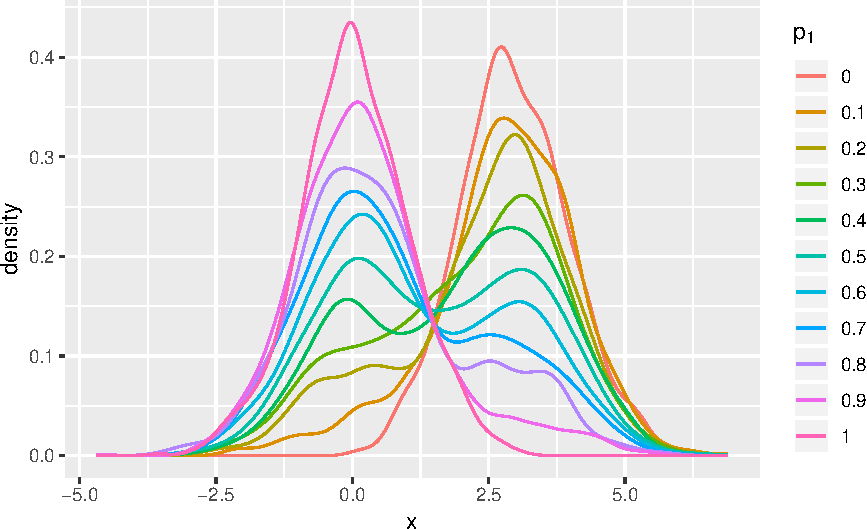
\includegraphics[width=0.7\linewidth]{statistical-computing_files/figure-latex/bimodal-1} 

}

\caption{Mixture normal random number for each mixing probability}\label{fig:bimodal}
\end{figure}

As \(p_1\) becomes larger to \(1\), the distribution becomes \(N(0, 1)\). On the contrary, \(p_1 = 0\) results in \(N(3, 1)\).

\hypertarget{multivariate-normal-random-vector}{%
\section{Multivariate Normal Random Vector}\label{multivariate-normal-random-vector}}

\BeginKnitrBlock{definition}[Multivariate normal random vector]
\protect\hypertarget{def:mvn}{}{\label{def:mvn} \iffalse (Multivariate normal random vector) \fi{} }A random vector \(\mathbf{X} = (X_1, \ldots, X_p)^T\) follows multivariate normal distribution if

\[f(\mathbf{x}) = \frac{1}{(2\pi)^{\frac{p}{2}\lvert \Sigma \rvert}} \exp \bigg[ -\frac{1}{2}(\mathbf{x} \boldsymbol\mu)^T \Sigma^{-1}(\mathbf{x} \boldsymbol\mu) \bigg]\]
\EndKnitrBlock{definition}

\BeginKnitrBlock{remark}
\iffalse{} {Remark. } \fi{}Let \(\mathbf{Z} \sim MVN(\mathbf{0}, I)\). Then

\begin{equation}
  \Sigma^{\frac{1}{2}}\mathbf{Z} + \boldsymbol\mu \sim MVN(\boldsymbol\mu, \Sigma)
  \label{eq:stdmvn}
\end{equation}
\EndKnitrBlock{remark}

From this remark, we get to generate \emph{standard normal random vector}.

\hypertarget{spectral-decomposition-method}{%
\subsection{Spectral decomposition method}\label{spectral-decomposition-method}}

Note that covariance matrix is symmetric.

\BeginKnitrBlock{theorem}[Spectral decomposition]
\protect\hypertarget{thm:covspec}{}{\label{thm:covspec} \iffalse (Spectral decomposition) \fi{} }Suppose that \(\Sigma\) is symmetric. Then

\[\Sigma = P \Lambda P^T\]

where \((\mathbf{v}_j, \lambda_j)\) corresponding eigenvector-eigenvalue

\[
\begin{cases}
  P = \begin{bmatrix} \mathbf{v}_1 & \cdots & \mathbf{v}_p \end{bmatrix} \in \mathbb{R}^{p \times p} \:\text{orthogonal} \\
  \Lambda = diag(\lambda_1, \ldots, \lambda_p)
\end{cases}
\]
\EndKnitrBlock{theorem}

\BeginKnitrBlock{corollary}
\protect\hypertarget{cor:specsqrt}{}{\label{cor:specsqrt} }Suppose that \(\Sigma\) is symmetric. Then

\[\Sigma^{\frac{1}{2}} = P \Lambda^{\frac{1}{2}} P^T\]

where \(\Lambda^{\frac{1}{2}} = diag(\sqrt{\lambda_1}, \ldots, \sqrt{\lambda_p})\)
\EndKnitrBlock{corollary}

\texttt{eigen()} performs spectral decomposition. \texttt{\$values} has eigenvalues and \texttt{\$vectors} has eigenvectors. We first generate matrix that consists of standard normal random vector:

\[
\begin{bmatrix}
  Z_{11} & Z_{12} & \cdots & Z_{1p} \\
  Z_{21} & Z_{22} & \cdots & Z_{2p} \\
  \vdots & \vdots & \vdots & \vdots \\
  Z_{n1} & Z_{n2} & \cdots & Z_{np}
\end{bmatrix}
\]

Denote that each observation is row. To use Equation \eqref{eq:stdmvn}, we should multiply \(\Sigma^{\frac{1}{2}}\) behind this matrix, not in front of. \(\boldsymbol\mu\) matrix should be also made to matrix, in form of

\[
\begin{bmatrix}
  \mu_{11} & \mu_{12} & \cdots & \mu_{1p} \\
  \mu_{11} & \mu_{22} & \cdots & \mu_{1p} \\
  \vdots & \vdots & \vdots & \vdots \\
  \mu_{11} & Z_{n2} & \cdots & \mu_{1p}
\end{bmatrix} \in \mathbb{R}^{n \times p}
\]

\begin{Shaded}
\begin{Highlighting}[]
\NormalTok{rmvn_eigen <-}\StringTok{ }\ControlFlowTok{function}\NormalTok{(n, mu, sig) \{}
\NormalTok{  d <-}\StringTok{ }\KeywordTok{length}\NormalTok{(mu)}
\NormalTok{  ev <-}\StringTok{ }\KeywordTok{eigen}\NormalTok{(sig, }\DataTypeTok{symmetric =} \OtherTok{TRUE}\NormalTok{)}
\NormalTok{  lambda <-}\StringTok{ }\NormalTok{ev}\OperatorTok{$}\NormalTok{values}
\NormalTok{  P <-}\StringTok{ }\NormalTok{ev}\OperatorTok{$}\NormalTok{vectors}
\NormalTok{  sig2 <-}\StringTok{ }\NormalTok{P }\OperatorTok\StringTok{ }\KeywordTok{diag}\NormalTok{(}\KeywordTok{sqrt}\NormalTok{(lambda)) }\OperatorTok\StringTok{ }\KeywordTok{t}\NormalTok{(P)}
\NormalTok{  Z <-}\StringTok{ }\KeywordTok{matrix}\NormalTok{(}\KeywordTok{rnorm}\NormalTok{(n }\OperatorTok{*}\StringTok{ }\NormalTok{d), }\DataTypeTok{nrow =}\NormalTok{ n, }\DataTypeTok{ncol =}\NormalTok{ d)}
\NormalTok{  X <-}\StringTok{ }\NormalTok{Z }\OperatorTok\StringTok{ }\NormalTok{sig2 }\OperatorTok{+}\StringTok{ }\KeywordTok{matrix}\NormalTok{(mu, }\DataTypeTok{nrow =}\NormalTok{ n, }\DataTypeTok{ncol =}\NormalTok{ d, }\DataTypeTok{byrow =} \OtherTok{TRUE}\NormalTok{)}
  \KeywordTok{colnames}\NormalTok{(X) <-}\StringTok{ }\KeywordTok{paste0}\NormalTok{(}\StringTok{"x"}\NormalTok{, }\DecValTok{1}\OperatorTok{:}\NormalTok{d)}
\NormalTok{  X }\OperatorTok\StringTok{ }\KeywordTok{tbl_df}\NormalTok{()}
\NormalTok{\}}
\end{Highlighting}
\end{Shaded}

\begin{Shaded}
\begin{Highlighting}[]
\CommentTok{# mean vector -------------------------------}
\NormalTok{mu <-}\StringTok{ }\KeywordTok{c}\NormalTok{(}\DecValTok{0}\NormalTok{, }\DecValTok{1}\NormalTok{, }\DecValTok{2}\NormalTok{)}
\CommentTok{# symmetric matrix --------------------------}
\NormalTok{sig <-}\StringTok{ }\KeywordTok{matrix}\NormalTok{(}\KeywordTok{numeric}\NormalTok{(}\DecValTok{9}\NormalTok{), }\DataTypeTok{nrow =} \DecValTok{3}\NormalTok{, }\DataTypeTok{ncol =} \DecValTok{3}\NormalTok{)}
\KeywordTok{diag}\NormalTok{(sig) <-}\StringTok{ }\KeywordTok{rep}\NormalTok{(}\DecValTok{1}\NormalTok{, }\DecValTok{3}\NormalTok{)}
\NormalTok{sig[}\KeywordTok{lower.tri}\NormalTok{(sig)] <-}\StringTok{ }\KeywordTok{c}\NormalTok{(}\OperatorTok{-}\NormalTok{.}\DecValTok{5}\NormalTok{, }\FloatTok{.5}\NormalTok{, }\FloatTok{-.5}\NormalTok{) }\OperatorTok{*}\StringTok{ }\DecValTok{2}
\NormalTok{sig <-}\StringTok{ }\NormalTok{(sig }\OperatorTok{+}\StringTok{ }\KeywordTok{t}\NormalTok{(sig)) }\OperatorTok{/}\StringTok{ }\DecValTok{2}
\end{Highlighting}
\end{Shaded}

Generate

\[\mathbf{X}_i \sim MVN\bigg((0, 1, 2), \begin{bmatrix} 1&-0.5&0.5 \\ -0.5&1&-0.5 \\ 0.5&-0.5&1 \\ \end{bmatrix}\bigg)\]

\begin{Shaded}
\begin{Highlighting}[]
\NormalTok{(mvn3 <-}\StringTok{ }\KeywordTok{rmvn_eigen}\NormalTok{(}\DecValTok{1000}\NormalTok{, }\DataTypeTok{mu =}\NormalTok{ mu, }\DataTypeTok{sig =}\NormalTok{ sig))}
\CommentTok{#> # A tibble: 1,000 x 3}
\CommentTok{#>         x1       x2    x3}
\CommentTok{#>      <dbl>    <dbl> <dbl>}
\CommentTok{#>  1 -0.168   1.41    1.80 }
\CommentTok{#>  2  1.39   -0.00942 2.40 }
\CommentTok{#>  3 -0.710   1.30    1.37 }
\CommentTok{#>  4  0.0314  2.04    1.80 }
\CommentTok{#>  5  0.177   0.568   1.71 }
\CommentTok{#>  6 -0.960   1.23    1.61 }
\CommentTok{#>  7 -1.01    1.28    0.106}
\CommentTok{#>  8  0.272   0.0842  2.12 }
\CommentTok{#>  9  0.148   1.63    2.53 }
\CommentTok{#> 10 -1.24    1.53    1.28 }
\CommentTok{#> # ... with 990 more rows}
\end{Highlighting}
\end{Shaded}

\begin{Shaded}
\begin{Highlighting}[]
\NormalTok{mvn3 }\OperatorTok\StringTok{ }
\StringTok{  }\NormalTok{GGally}\OperatorTok{::}\KeywordTok{ggpairs}\NormalTok{(}
    \DataTypeTok{lower =} \KeywordTok{list}\NormalTok{(}\DataTypeTok{continuous =}\NormalTok{ GGally}\OperatorTok{::}\KeywordTok{wrap}\NormalTok{(gg_scatter, }\DataTypeTok{size =} \DecValTok{1}\NormalTok{))}
\NormalTok{  )}
\CommentTok{#> Registered S3 method overwritten by 'GGally':}
\CommentTok{#>   method from   }
\CommentTok{#>   +.gg   ggplot2}
\end{Highlighting}
\end{Shaded}

\begin{figure}[H]

{\centering 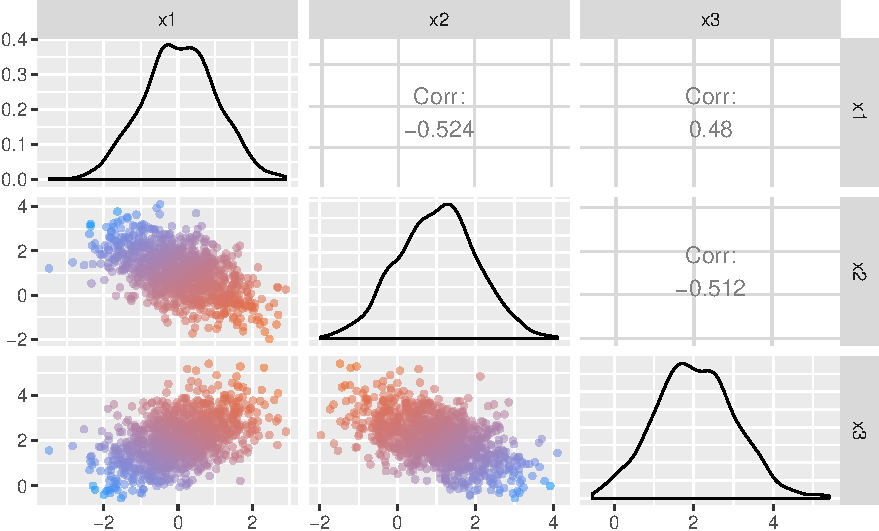
\includegraphics[width=0.7\linewidth]{statistical-computing_files/figure-latex/mvneigen-1} 

}

\caption{Multivariate normal random vector - spectral decomposition method}\label{fig:mvneigen}
\end{figure}

\hypertarget{singular-value-decomposition}{%
\subsection{Singular value decomposition}\label{singular-value-decomposition}}

SVD can be said to be a kind of generalization of spectral decomposition. This method can be used for any matrix, i.e.~non-symmetric matrix. For \(\Sigma\), SVD and spectral decomposition is equivalent. However, SVD does not account for symmetric property, so this method is less efficient compared to spectral decomposition.

\begin{Shaded}
\begin{Highlighting}[]
\NormalTok{rmvn_svd <-}\StringTok{ }\ControlFlowTok{function}\NormalTok{(n, mu, sig) \{}
\NormalTok{  d <-}\StringTok{ }\KeywordTok{length}\NormalTok{(mu)}
\NormalTok{  S <-}\StringTok{ }\KeywordTok{svd}\NormalTok{(sig)}
\NormalTok{  sig2 <-}\StringTok{ }\NormalTok{S}\OperatorTok{$}\NormalTok{u }\OperatorTok\StringTok{ }\KeywordTok{diag}\NormalTok{(}\KeywordTok{sqrt}\NormalTok{(S}\OperatorTok{$}\NormalTok{d)) }\OperatorTok\StringTok{ }\KeywordTok{t}\NormalTok{(S}\OperatorTok{$}\NormalTok{v)}
\NormalTok{  Z <-}\StringTok{ }\KeywordTok{matrix}\NormalTok{(}\KeywordTok{rnorm}\NormalTok{(n }\OperatorTok{*}\StringTok{ }\NormalTok{d), }\DataTypeTok{nrow =}\NormalTok{ n, }\DataTypeTok{ncol =}\NormalTok{ d)}
\NormalTok{  X <-}\StringTok{ }\NormalTok{Z }\OperatorTok\StringTok{ }\NormalTok{sig2 }\OperatorTok{+}\StringTok{ }\KeywordTok{matrix}\NormalTok{(mu, }\DataTypeTok{nrow =}\NormalTok{ n, }\DataTypeTok{ncol =}\NormalTok{ d, }\DataTypeTok{byrow =} \OtherTok{TRUE}\NormalTok{)}
  \KeywordTok{colnames}\NormalTok{(X) <-}\StringTok{ }\KeywordTok{paste0}\NormalTok{(}\StringTok{"x"}\NormalTok{, }\DecValTok{1}\OperatorTok{:}\NormalTok{d)}
\NormalTok{  X }\OperatorTok\StringTok{ }\KeywordTok{tbl_df}\NormalTok{()}
\NormalTok{\}}
\end{Highlighting}
\end{Shaded}

\begin{figure}[H]

{\centering 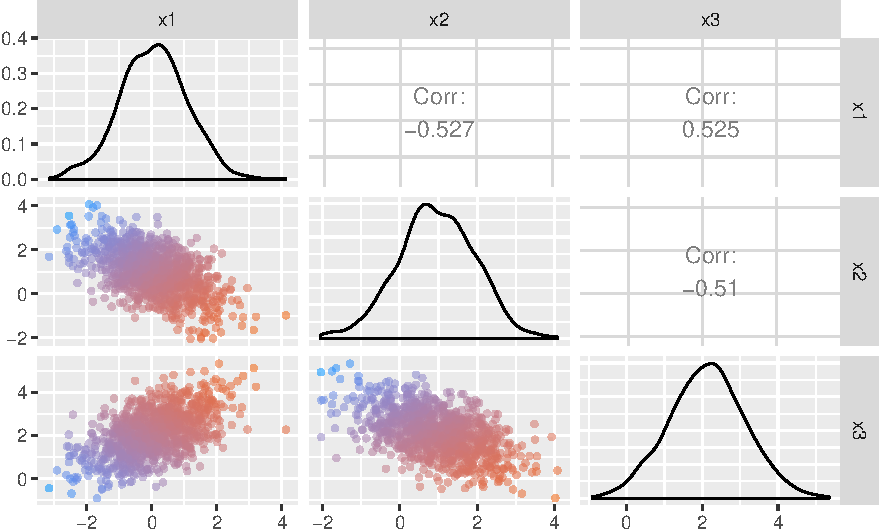
\includegraphics[width=0.7\linewidth]{statistical-computing_files/figure-latex/mvnsvd-1} 

}

\caption{Multivariate normal random vector - svd}\label{fig:mvnsvd}
\end{figure}

\hypertarget{choleski-decomposition}{%
\subsection{Choleski decomposition}\label{choleski-decomposition}}

\BeginKnitrBlock{theorem}[Cholesky decomposition]
\protect\hypertarget{thm:covchol}{}{\label{thm:covchol} \iffalse (Cholesky decomposition) \fi{} }Suppose that \(\Sigma\) is symmetric and positive definite. Then

\[\Sigma = Q^T Q\]

where \(Q\) is an upper triangular matrix.
\EndKnitrBlock{theorem}

\BeginKnitrBlock{corollary}
\protect\hypertarget{cor:mvnchol2}{}{\label{cor:mvnchol2} }Suppose that \(\Sigma\) is symmetric and positive definite. For cholesky decomposition \ref{thm:covchol}, define

\[\Sigma^{\frac{1}{2}} = Q\]
\EndKnitrBlock{corollary}

\texttt{chol()} computes cholesky decomposition. In \texttt{R}, it gives upper triangular \(Q\). Since some statements cholesky decomposition by \(\Sigma = LL^T\) with lower triangular matrix, try not to confuse.

\begin{Shaded}
\begin{Highlighting}[]
\NormalTok{rmvn_chol <-}\StringTok{ }\ControlFlowTok{function}\NormalTok{(n, mu, sig) \{}
\NormalTok{  d <-}\StringTok{ }\KeywordTok{length}\NormalTok{(mu)}
\NormalTok{  sig2 <-}\StringTok{ }\KeywordTok{chol}\NormalTok{(sig)}
\NormalTok{  Z <-}\StringTok{ }\KeywordTok{matrix}\NormalTok{(}\KeywordTok{rnorm}\NormalTok{(n }\OperatorTok{*}\StringTok{ }\NormalTok{d), }\DataTypeTok{nrow =}\NormalTok{ n, }\DataTypeTok{ncol =}\NormalTok{ d)}
\NormalTok{  X <-}\StringTok{ }\NormalTok{Z }\OperatorTok\StringTok{ }\NormalTok{sig2 }\OperatorTok{+}\StringTok{ }\KeywordTok{matrix}\NormalTok{(mu, }\DataTypeTok{nrow =}\NormalTok{ n, }\DataTypeTok{ncol =}\NormalTok{ d, }\DataTypeTok{byrow =} \OtherTok{TRUE}\NormalTok{)}
  \KeywordTok{colnames}\NormalTok{(X) <-}\StringTok{ }\KeywordTok{paste0}\NormalTok{(}\StringTok{"x"}\NormalTok{, }\DecValTok{1}\OperatorTok{:}\NormalTok{d)}
\NormalTok{  X }\OperatorTok\StringTok{ }\KeywordTok{tbl_df}\NormalTok{()}
\NormalTok{\}}
\end{Highlighting}
\end{Shaded}

\begin{figure}[H]

{\centering 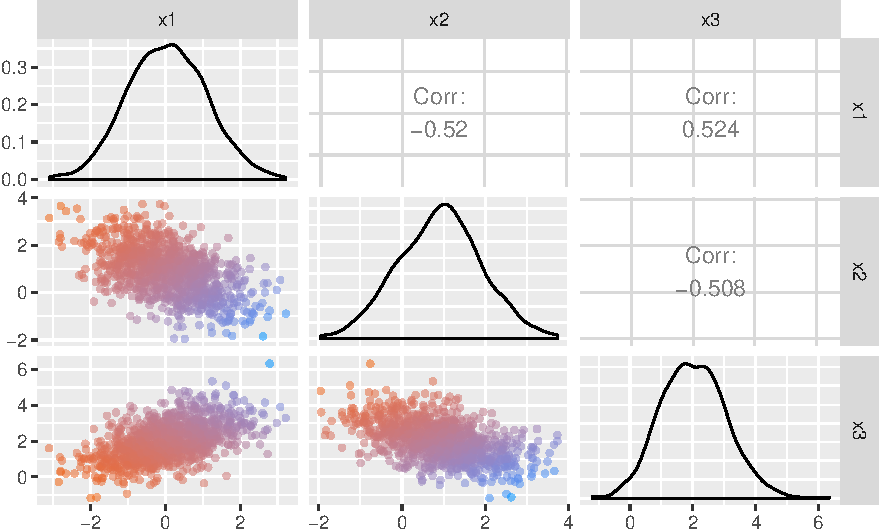
\includegraphics[width=0.7\linewidth]{statistical-computing_files/figure-latex/mvnchol-1} 

}

\caption{Multivariate normal random vector - cholesky decomposition}\label{fig:mvnchol}
\end{figure}

\hypertarget{stochastic-processes}{%
\section{Stochastic Processes}\label{stochastic-processes}}

\BeginKnitrBlock{definition}[Stochastic process]
\protect\hypertarget{def:stoc}{}{\label{def:stoc} \iffalse (Stochastic process) \fi{} }A stochastic process is a collection \(\{ X(t) : t \in T \}\) of random variables indexed by the set \(T\). The index set \(T\) could be discrete or continous.

A State space is called te set of possible values that \(X(t)\) can take.
\EndKnitrBlock{definition}

\BeginKnitrBlock{definition}[Discrete Time Markov Chain]
\protect\hypertarget{def:dmc}{}{\label{def:dmc} \iffalse (Discrete Time Markov Chain) \fi{} }\(\{ X_n : n = 0, 1, 2, \ldots \}\) is a Discrete time markov chain on \(S\) if and only if

\begin{enumerate}
  \item $S$ is at most countable
  \item Markov property $P(X_{n + 1} = j \mid X_n = i, X_{n - 1} = i_{n - 1}, \ldots, X_0 = i_0) = P(X_{n + 1} = j \mid X_n = i) = P_{ij}$
\end{enumerate}

If \(P_{ij}\) is fixed, then \(\{ X_n \}\) is called time homogeneous. Otherwise, it is called nonhomogeneous.
\EndKnitrBlock{definition}

\BeginKnitrBlock{definition}[Random walk model]
\protect\hypertarget{def:rwm}{}{\label{def:rwm} \iffalse (Random walk model) \fi{} }Let \(\{ Y_n : n \in \mathbb{N} \}\) be an IID process on \(S\) s.t.

\[P(Y_n = k) = p_k\]

Define

\[
S_n := \begin{cases}
  0 & n = 0 \\
  S_0 + Y_1 + \cdots + Y_n & n \in \mathbb{N}
\end{cases}
\]
\EndKnitrBlock{definition}

\hypertarget{gamblers-ruin-model}{%
\subsection{Gambler's ruin model}\label{gamblers-ruin-model}}

\BeginKnitrBlock{definition}[Gambler's ruin model]
\protect\hypertarget{def:gambler}{}{\label{def:gambler} \iffalse (Gambler's ruin model) \fi{} }Let \(\{ Y_n : n \in \mathbb{N} \}\) be a process on \(\{ -1, 1 \}\) s.t.

\[P(Y_n = 1) = p, \quad P(Y_n = -1) = 1 - p\]

Define

\[
X_n := \begin{cases}
  a & n = 0 \\
  a + Y_1 + \cdots + Y_n & n \in \mathbb{N}
\end{cases}
\]
\EndKnitrBlock{definition}

\BeginKnitrBlock{example}[Gambling with coin]
\protect\hypertarget{exm:gamble}{}{\label{exm:gamble} \iffalse (Gambling with coin) \fi{} }Suppose that A and B each start with a stake of \$10, and bet \$1 on consecutive coin flips. The game ends when either one of the players has all the money. Let \(S_n\) be the fortune of player A at time \(n\) Then \(\{ S_n, n \ge 0 \}\) is a symmetric random walk with absorbing barriers at 0 and 20. Simulate a realization of the process \(\{ S_n, n \ge 0 \}\) and plot \(S_n\) vs the time index from time \(0\) until a barrier is reached.
\EndKnitrBlock{example}

Here we have

\[P(Y_n = 1) = P(Y_n = -1) = \frac{1}{2}\]

\[
S_n := \begin{cases}
  10 & n = 0 \\
  10 + Y_1 + \cdots + Y_n & n \in \mathbb{N}
\end{cases}
\]

\begin{Shaded}
\begin{Highlighting}[]
\NormalTok{gambling <-}\StringTok{ }\ControlFlowTok{function}\NormalTok{(}\DataTypeTok{begin =} \DecValTok{10}\NormalTok{, }\DataTypeTok{betting =} \DecValTok{1}\NormalTok{, }\DataTypeTok{prob =} \FloatTok{.5}\NormalTok{) \{}
\NormalTok{  N <-}\StringTok{ }\NormalTok{begin }\OperatorTok{*}\StringTok{ }\DecValTok{2}
\NormalTok{  sa <-}\StringTok{ }\NormalTok{begin}
\NormalTok{  record <-}\StringTok{ }\KeywordTok{tibble}\NormalTok{(}\DataTypeTok{a =}\NormalTok{ begin, }\DataTypeTok{b =}\NormalTok{ begin)}
  \ControlFlowTok{while}\NormalTok{(}\KeywordTok{all}\NormalTok{(record }\OperatorTok{>}\StringTok{ }\DecValTok{0}\NormalTok{)) \{}
\NormalTok{    sa <-}\StringTok{ }\KeywordTok{ifelse}\NormalTok{(}\KeywordTok{runif}\NormalTok{(}\DecValTok{1}\NormalTok{) }\OperatorTok{<=}\StringTok{ }\NormalTok{prob, sa }\OperatorTok{+}\StringTok{ }\NormalTok{betting, sa }\OperatorTok{-}\StringTok{ }\NormalTok{betting)}
\NormalTok{    record <-}
\StringTok{      }\NormalTok{record }\OperatorTok\StringTok{ }
\StringTok{      }\KeywordTok{bind_rows}\NormalTok{(}\KeywordTok{c}\NormalTok{(}\DataTypeTok{a =}\NormalTok{ sa, }\DataTypeTok{b =}\NormalTok{ N }\OperatorTok{-}\StringTok{ }\NormalTok{sa))}
    \ControlFlowTok{if}\NormalTok{ (sa }\OperatorTok{==}\StringTok{ }\NormalTok{N) }\ControlFlowTok{break}\NormalTok{()}
\NormalTok{  \}}
\NormalTok{  record }\OperatorTok\StringTok{ }
\StringTok{    }\KeywordTok{mutate}\NormalTok{(}\DataTypeTok{idx =} \DecValTok{1}\OperatorTok{:}\KeywordTok{n}\NormalTok{()) }\OperatorTok\StringTok{ }
\StringTok{    }\KeywordTok{select}\NormalTok{(idx, a, b)}
\NormalTok{\}}
\end{Highlighting}
\end{Shaded}

\begin{Shaded}
\begin{Highlighting}[]
\KeywordTok{gambling}\NormalTok{(}\DataTypeTok{begin =} \DecValTok{10}\NormalTok{, }\DataTypeTok{betting =} \DecValTok{1}\NormalTok{, }\DataTypeTok{prob =} \FloatTok{.5}\NormalTok{) }\OperatorTok\StringTok{ }
\StringTok{  }\KeywordTok{gather}\NormalTok{(}\OperatorTok{-}\NormalTok{idx, }\DataTypeTok{key =} \StringTok{"player"}\NormalTok{, }\DataTypeTok{value =} \StringTok{"fortune"}\NormalTok{) }\OperatorTok\StringTok{ }
\StringTok{  }\KeywordTok{ggplot}\NormalTok{(}\KeywordTok{aes}\NormalTok{(}\DataTypeTok{x =}\NormalTok{ idx, }\DataTypeTok{y =}\NormalTok{ fortune, }\DataTypeTok{colour =}\NormalTok{ player)) }\OperatorTok{+}
\StringTok{  }\KeywordTok{geom_path}\NormalTok{() }\OperatorTok{+}
\StringTok{  }\KeywordTok{geom_point}\NormalTok{(}\DataTypeTok{alpha =} \FloatTok{.5}\NormalTok{, }\DataTypeTok{size =} \DecValTok{1}\NormalTok{) }\OperatorTok{+}
\StringTok{  }\KeywordTok{geom_hline}\NormalTok{(}\DataTypeTok{yintercept =} \KeywordTok{c}\NormalTok{(}\DecValTok{0}\NormalTok{, }\DecValTok{20}\NormalTok{), }\DataTypeTok{col =} \KeywordTok{I}\NormalTok{(}\StringTok{"grey"}\NormalTok{)) }\OperatorTok{+}
\StringTok{  }\KeywordTok{labs}\NormalTok{(}
    \DataTypeTok{x =} \StringTok{"Betting"}\NormalTok{,}
    \DataTypeTok{y =} \StringTok{"Fortune"}
\NormalTok{  )}
\end{Highlighting}
\end{Shaded}

\begin{figure}[H]

{\centering 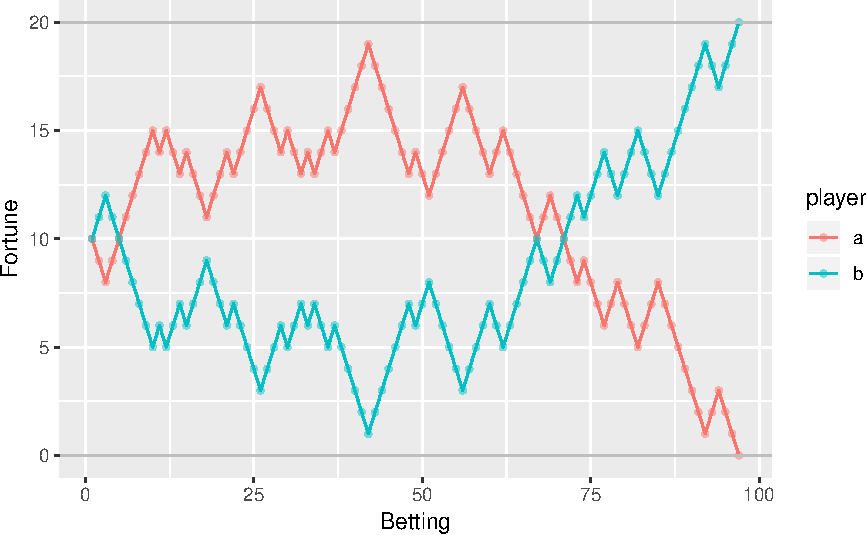
\includegraphics[width=0.7\linewidth]{statistical-computing_files/figure-latex/gambfig-1} 

}

\caption{Sample path of Gambler's ruin model}\label{fig:gambfig}
\end{figure}

In Figure \ref{fig:gambfig}, we can see the result of process with \(p = \frac{1}{2}\). In fact, this process with probability \(0.5\) is also called \emph{symmetric random walk}.

\hypertarget{homogeneous-poisson-process}{%
\subsection{Homogeneous poisson process}\label{homogeneous-poisson-process}}

\BeginKnitrBlock{definition}[Count process]
\protect\hypertarget{def:coutpr}{}{\label{def:coutpr} \iffalse (Count process) \fi{} }A stochastic process \(\{ N(t) : t \ge 0 \}\) where \(N(t)\) is total number of events that occur by time \(t\) is called counting process.

\begin{enumerate}
  \item $N(t) \ge 0$
  \item $N(t) \in \mathbb{Z}$
  \item $s \le t \Rightarrow N(s) \le N(t)$
  \item For $s < t$, $N(t) - N(s) = \:\text{the number of events that occur in}\: (s,t]$
\end{enumerate}
\EndKnitrBlock{definition}

\emph{Poisson process} is one of this counting process.

\BeginKnitrBlock{definition}[Poisson process]
\protect\hypertarget{def:ppdef}{}{\label{def:ppdef} \iffalse (Poisson process) \fi{} }The counting process \(\{ N(t), t \ge 0 \}\) is said to be a Poisson process with rate \(\lambda >0\)

\begin{enumerate}
  \item $N(0) = 0$
  \item $N(t) \perp\!\!\!\perp N(t + s) - N(t)$
  \item Distribution of $N(t + s) - N(t)$ is the same for all values of $t$
  \item $\lim\limits_{h \rightarrow 0} \frac{P(N(h) = 1)}{h} = \lambda$
  \item $\lim\limits_{h \rightarrow 0} \frac{P(N(h) \ge 2)}{h} = 0$
\end{enumerate}
\EndKnitrBlock{definition}

\BeginKnitrBlock{remark}
\iffalse{} {Remark. } \fi{}\[\{ N(t), t \ge 0 \} \sim PP(\lambda) \Rightarrow N(t) \sim Poisson(\lambda t)\]
\EndKnitrBlock{remark}

We can generate Poisson process using this relationship. However, it is slow. Thus, we find another way.

\BeginKnitrBlock{theorem}[Campbell's Theorem]
\protect\hypertarget{thm:campbell}{}{\label{thm:campbell} \iffalse (Campbell's Theorem) \fi{} }Let \(\{ N(t), t \ge 0 \} \sim PP(\lambda)\), let \(X_t\) be the interarrival time, and let \(S_{t}\) be the waiting time until \(t\)-th event, i.e.~\(S_t := \sum_{i = 1}^t X_i\). Then

\[S_1, S_2, \ldots, S_n \mid N(t) = n \stackrel{d}{=} (U_{(1)}, U_{(2)}, \ldots, U_{(n)})\]

where \(U_i \sim unif(0, t)\).
\EndKnitrBlock{theorem}

This Campbell's theorem gives solution to the PP generation.

\begin{algorithm}[H] \label{alg:algpp}
  \SetAlgoLined
  \SetKwInOut{Input}{input}
  \SetKwInOut{Output}{output}
  \Input{end time $T$}
  Generate $N \sim Poisson(\lambda T)$\;
  For $N$, generate $U_1, \ldots, U_N \stackrel{iid}{\sim} unif(0, T)$\;
  Sort $U_1, \ldots, U_N$ in ascending order, i.e. $\{ U_{(1)}, \ldots, U_{(N)} \}$\;
  Set $S_1 = U_{(1)}, \ldots, S_N = U_{(N)}$\;
  \Output{$\begin{bmatrix} 1 & S_1 \\ 2 & S_2 \\ \cdots & \cdots \\ N & S_n \end{bmatrix}$ \\ $\Rightarrow \{ N(S_n) \} \sim PP(\lambda) \: \text{on} \: [0, T]$}
  \caption{Fast algorithm for Poisson Process}
\end{algorithm}

\begin{Shaded}
\begin{Highlighting}[]
\NormalTok{rpp <-}\StringTok{ }\ControlFlowTok{function}\NormalTok{(lambda, t0) \{}
\NormalTok{  N <-}\StringTok{ }\KeywordTok{rpois}\NormalTok{(}\DecValTok{1}\NormalTok{, }\DataTypeTok{lambda =}\NormalTok{ lambda }\OperatorTok{*}\StringTok{ }\NormalTok{t0)}
  \KeywordTok{tibble}\NormalTok{(}\DataTypeTok{sn =} \KeywordTok{runif}\NormalTok{(N) }\OperatorTok{*}\StringTok{ }\NormalTok{t0) }\OperatorTok\StringTok{ }
\StringTok{    }\KeywordTok{arrange}\NormalTok{(sn) }\OperatorTok\StringTok{ }\CommentTok{# arrival time}
\StringTok{    }\KeywordTok{mutate}\NormalTok{(}\DataTypeTok{pp =} \DecValTok{1}\OperatorTok{:}\KeywordTok{n}\NormalTok{()) }\CommentTok{# N(sn) ~ PP}
\NormalTok{\}}
\end{Highlighting}
\end{Shaded}

\begin{Shaded}
\begin{Highlighting}[]
\KeywordTok{rpp}\NormalTok{(}\DataTypeTok{lambda =} \DecValTok{1}\NormalTok{, }\DataTypeTok{t0 =} \DecValTok{50}\NormalTok{) }\OperatorTok\StringTok{ }
\StringTok{  }\KeywordTok{mutate}\NormalTok{(}
    \DataTypeTok{true_mean =}\NormalTok{ sn, }\CommentTok{# sn * lambda}
    \DataTypeTok{true_sd =} \KeywordTok{sqrt}\NormalTok{(sn) }\CommentTok{# sn * lambda}
\NormalTok{  ) }\OperatorTok\StringTok{ }
\StringTok{  }\KeywordTok{ggplot}\NormalTok{(}\KeywordTok{aes}\NormalTok{(}\DataTypeTok{x =}\NormalTok{ sn)) }\OperatorTok{+}
\StringTok{  }\KeywordTok{geom_ribbon}\NormalTok{(}
    \KeywordTok{aes}\NormalTok{(}\DataTypeTok{ymin =}\NormalTok{ true_mean }\OperatorTok{-}\StringTok{ }\NormalTok{true_sd, }\DataTypeTok{ymax =}\NormalTok{ true_mean }\OperatorTok{+}\StringTok{ }\NormalTok{true_sd), }
    \DataTypeTok{fill =} \StringTok{"grey70"}\NormalTok{, }
    \DataTypeTok{alpha =} \FloatTok{.5}
\NormalTok{  ) }\OperatorTok{+}
\StringTok{  }\KeywordTok{geom_line}\NormalTok{(}\KeywordTok{aes}\NormalTok{(}\DataTypeTok{y =}\NormalTok{ true_mean), }\DataTypeTok{col =} \KeywordTok{I}\NormalTok{(}\StringTok{"white"}\NormalTok{), }\DataTypeTok{size =} \DecValTok{2}\NormalTok{) }\OperatorTok{+}
\StringTok{  }\KeywordTok{geom_path}\NormalTok{(}\KeywordTok{aes}\NormalTok{(}\DataTypeTok{y =}\NormalTok{ pp)) }\OperatorTok{+}
\StringTok{  }\KeywordTok{labs}\NormalTok{(}
    \DataTypeTok{x =} \StringTok{"t"}\NormalTok{,}
    \DataTypeTok{y =} \KeywordTok{expression}\NormalTok{(}\KeywordTok{N}\NormalTok{(t))}
\NormalTok{  )}
\end{Highlighting}
\end{Shaded}

\begin{figure}[H]

{\centering 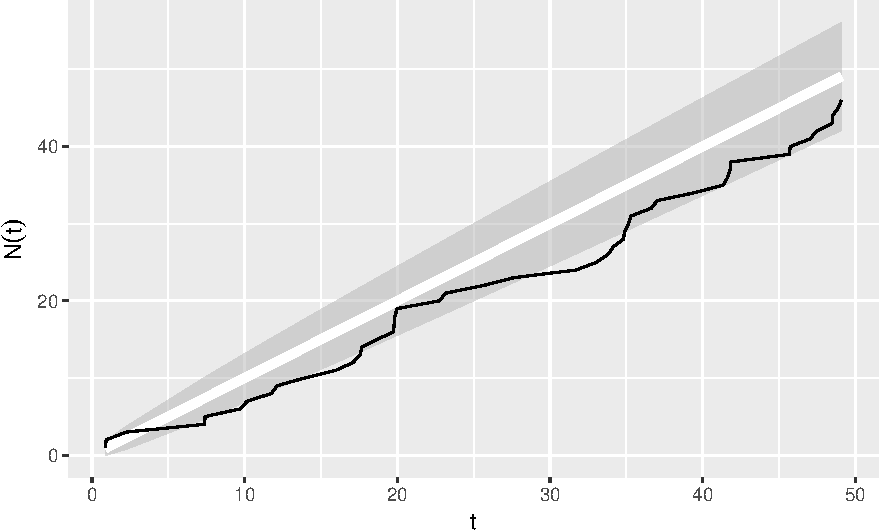
\includegraphics[width=0.7\linewidth]{statistical-computing_files/figure-latex/ppfig-1} 

}

\caption{Sample path of Poisson process}\label{fig:ppfig}
\end{figure}

\hypertarget{nonhomogeneous-poisson-process}{%
\subsection{Nonhomogeneous poisson process}\label{nonhomogeneous-poisson-process}}

Last section, what we have seen was homogeneous PP whose distribution does not depend on \(t\). On the other hand, this condition can be broken.

\BeginKnitrBlock{definition}[Nonhomogeneous Poisson Process]
\protect\hypertarget{def:npp}{}{\label{def:npp} \iffalse (Nonhomogeneous Poisson Process) \fi{} }The counting process \(\{ N(t), t \ge 0 \}\) is said to be a Nonhomogeneous Poisson process with rate \(\lambda(t) >0\) if the third condition does not hold.

\begin{enumerate}
  \item $N(0) = 0$
  \item $N(t) \perp\!\!\!\perp N(t + s) - N(t)$
  \item $\lim\limits_{h \rightarrow 0} \frac{P(N(h) = 1)}{h} = \lambda$
  \item $\lim\limits_{h \rightarrow 0} \frac{P(N(h) \ge 2)}{h} = 0$
\end{enumerate}

\(\lambda(t)\) is called intensity at time \(t\).

\(m(t) := \int_0^t \lambda(s) ds, t \ge 0\) is called mean-value function.
\EndKnitrBlock{definition}

We can generate this NPP by Bernoulli splitting, which is called \emph{thining approach}.

\BeginKnitrBlock{lemma}[Thinning approach]
\protect\hypertarget{lem:thin}{}{\label{lem:thin} \iffalse (Thinning approach) \fi{} }Choosing \(\lambda\) s.t. \(\forall t \le T \lambda(t) \le \lambda\). If an event of \(PP(\lambda)\) counted with

\[p(t) = \frac{\lambda(t)}{\lambda}\]

then the process follows \(NPP(\lambda(t))\) on \([0, T]\)
\EndKnitrBlock{lemma}

\begin{algorithm}[H] \label{alg:algnpp}
  \SetAlgoLined
  \SetKwInOut{Input}{input}
  \SetKwInOut{Output}{output}
  Set $t = 0, N = 0$\;
  \Repeat{$t > T$}{
    Generate $Y \sim Exp(\lambda)$\;
    Set $t \leftarrow t + Y$\;
    Generate $U \sim unif(0, 1)$\;
    \uIf{$U \le \frac{\lambda(t)}{\lambda}$}{
      Set $N \leftarrow N + 1$\;
      Set $S(N) \leftarrow t$\;
    }
  }
  \caption{Thinning algorithm}
\end{algorithm}

\begin{Shaded}
\begin{Highlighting}[]
\NormalTok{npp <-}\StringTok{ }\ControlFlowTok{function}\NormalTok{(lambda, t0, intensity) \{}
\NormalTok{  t <-}\StringTok{ }\DecValTok{0}
\NormalTok{  N <-}\StringTok{ }\DecValTok{0}
\NormalTok{  S <-}\StringTok{ }\KeywordTok{tibble}\NormalTok{(}\DataTypeTok{t =}\NormalTok{ t, }\DataTypeTok{N =}\NormalTok{ N)}
  \ControlFlowTok{while}\NormalTok{ (t }\OperatorTok{<=}\StringTok{ }\NormalTok{t0) \{}
\NormalTok{    t <-}\StringTok{ }\NormalTok{t }\OperatorTok{+}\StringTok{ }\KeywordTok{rexp}\NormalTok{(}\DecValTok{1}\NormalTok{, lambda)}
\NormalTok{    U <-}\StringTok{ }\KeywordTok{runif}\NormalTok{(}\DecValTok{1}\NormalTok{)}
    \ControlFlowTok{if}\NormalTok{ ( U }\OperatorTok{<=}\StringTok{ }\KeywordTok{intensity}\NormalTok{(t) }\OperatorTok{/}\StringTok{ }\NormalTok{lambda) \{}
\NormalTok{      N <-}\StringTok{ }\NormalTok{N }\OperatorTok{+}\StringTok{ }\DecValTok{1}
\NormalTok{      S <-}
\StringTok{        }\NormalTok{S }\OperatorTok\StringTok{ }
\StringTok{        }\KeywordTok{bind_rows}\NormalTok{(}\KeywordTok{tibble}\NormalTok{(}\DataTypeTok{t =}\NormalTok{ t, }\DataTypeTok{N =}\NormalTok{ N))}
\NormalTok{    \}}
\NormalTok{  \}}
\NormalTok{  S }\OperatorTok\StringTok{ }\KeywordTok{slice}\NormalTok{(}\OperatorTok{-}\DecValTok{1}\NormalTok{)}
\NormalTok{\}}
\end{Highlighting}
\end{Shaded}

\begin{Shaded}
\begin{Highlighting}[]
\NormalTok{intensity <-}\StringTok{ }\ControlFlowTok{function}\NormalTok{(x) \{}
\NormalTok{  tt <-}\StringTok{ }\NormalTok{x }\OperatorTok\StringTok{ }\DecValTok{480}
\NormalTok{  rate <-}
\StringTok{    }\KeywordTok{case_when}\NormalTok{(}
\NormalTok{      tt }\OperatorTok{>=}\StringTok{ }\DecValTok{0} \OperatorTok{&&}\StringTok{ }\NormalTok{tt }\OperatorTok{<=}\StringTok{ }\DecValTok{120} \OperatorTok{~}\StringTok{ }\FloatTok{.5}\NormalTok{,}
\NormalTok{      tt }\OperatorTok{>}\StringTok{ }\DecValTok{120} \OperatorTok{&&}\StringTok{ }\NormalTok{tt }\OperatorTok{<=}\StringTok{ }\DecValTok{240} \OperatorTok{~}\StringTok{ }\DecValTok{1}\NormalTok{,}
\NormalTok{      tt }\OperatorTok{>}\StringTok{ }\DecValTok{240} \OperatorTok{&&}\StringTok{ }\NormalTok{tt }\OperatorTok{<=}\StringTok{ }\DecValTok{360} \OperatorTok{~}\StringTok{ }\DecValTok{2}\NormalTok{,}
\NormalTok{      tt }\OperatorTok{>}\StringTok{ }\DecValTok{360} \OperatorTok{&&}\StringTok{ }\NormalTok{tt }\OperatorTok{<=}\StringTok{ }\DecValTok{480} \OperatorTok{~}\StringTok{ }\FloatTok{1.5}
\NormalTok{    )}
\NormalTok{  rate}
\NormalTok{\}}
\CommentTok{#--------------------------}
\KeywordTok{npp}\NormalTok{(}\DecValTok{2}\NormalTok{, }\DecValTok{480}\NormalTok{, }\DataTypeTok{intensity =}\NormalTok{ intensity) }\OperatorTok\StringTok{ }
\StringTok{  }\KeywordTok{ggplot}\NormalTok{(}\KeywordTok{aes}\NormalTok{(}\DataTypeTok{x =}\NormalTok{ t, }\DataTypeTok{y =}\NormalTok{ N)) }\OperatorTok{+}
\StringTok{  }\KeywordTok{geom_path}\NormalTok{()}
\end{Highlighting}
\end{Shaded}

\begin{figure}[H]

{\centering 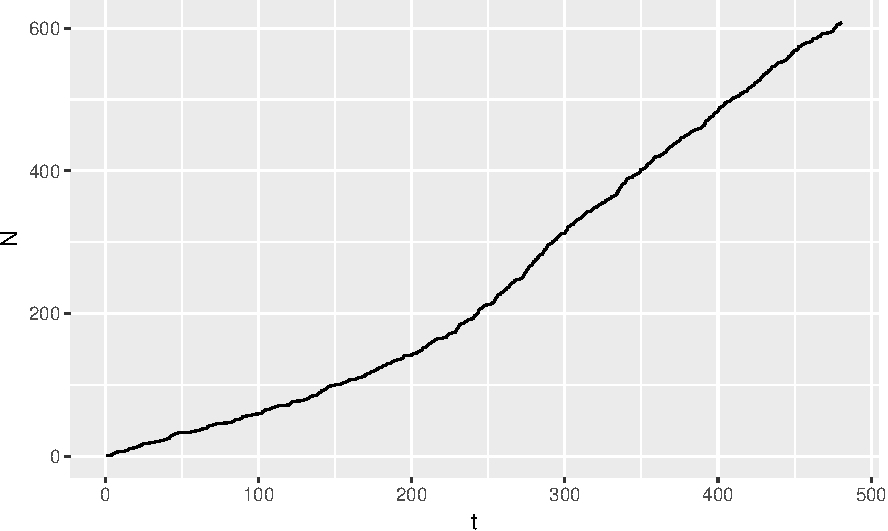
\includegraphics[width=0.7\linewidth]{statistical-computing_files/figure-latex/nppfig-1} 

}

\caption{Sample path of nonhomogeneous poisson process}\label{fig:nppfig}
\end{figure}

\hypertarget{mcint}{%
\chapter{Monte Carlo Integration and Variance Reduction}\label{mcint}}

\hypertarget{monte-carlo-integration}{%
\section{Monte Carlo Integration}\label{monte-carlo-integration}}

Consider integration problem of a integrable function \(g(x)\). We want to compute

\[\theta \equiv \int_a^b g(x) dx\]

For instance, standard normal cdf.

\BeginKnitrBlock{example}[Standard normal cdf]
\protect\hypertarget{exm:mcex}{}{\label{exm:mcex} \iffalse (Standard normal cdf) \fi{} }Compute values for

\[\Phi(x) = \int_{-\infty}^x \frac{1}{\sqrt{2\pi}}\exp\bigg(-\frac{t^2}{2}\bigg)dt\]
\EndKnitrBlock{example}

It might be impossible to compute this integral with hand. So we implement \emph{simulation} concept here, based on the following theorems.

\BeginKnitrBlock{theorem}[Weak Law of Large Numbers]
\protect\hypertarget{thm:wlaw}{}{\label{thm:wlaw} \iffalse (Weak Law of Large Numbers) \fi{} }Suppose that \(X_1, \ldots, X_n \stackrel{iid}{\sim}(\mu, \sigma^2 < \infty)\). Then

\[\frac{1}{n}\sum_{i = 1}^n X_i \stackrel{p}{\rightarrow} \mu\]

Let \(g\) be a measurable function. Then

\[\frac{1}{n}\sum_{i = 1}^n g(X_i) \stackrel{p}{\rightarrow} g(\mu)\]
\EndKnitrBlock{theorem}

\BeginKnitrBlock{theorem}[Strong Law of Large Numbers]
\protect\hypertarget{thm:slaw}{}{\label{thm:slaw} \iffalse (Strong Law of Large Numbers) \fi{} }Suppose that \(X_1, \ldots, X_n \stackrel{iid}{\sim}(\mu, \sigma^2 < \infty)\). Then

\[\frac{1}{n}\sum_{i = 1}^n X_i \stackrel{a.s.}{\rightarrow} \mu\]

Let \(g\) be a measurable function. Then

\[\frac{1}{n}\sum_{i = 1}^n g(X_i) \stackrel{a.s.}{\rightarrow} g(\mu)\]
\EndKnitrBlock{theorem}

\hypertarget{simple-monte-carlo-estimator}{%
\subsection{Simple Monte Carlo estimator}\label{simple-monte-carlo-estimator}}

\BeginKnitrBlock{theorem}[Monte Carlo Integration]
\protect\hypertarget{thm:mcint}{}{\label{thm:mcint} \iffalse (Monte Carlo Integration) \fi{} }Consider integration \eqref{eq:muint}. This can be approximated via appropriate pdf \(f(x)\) by

\[\hat\theta_M = \frac{1}{N} \sum_{i = 1}^N g(X_i)\]
\EndKnitrBlock{theorem}

Suppose that we have a distribution \(f(x) = I_{spt g}(x)\), i.e.~\emph{uniform distribution}. Let \(spt g = (a, b)\).

\begin{equation}
  \begin{split}
    \theta & \equiv \int_{spt g} g(x) dx \\
    & = \int_a^b g(x) dx \\
    & = \int_0^1 g(a + (b - a)t)(b - a) dt \\
    & \equiv \int_0^1 h(t) dt \\
    & = \int_0^1 h(t) I_{(a, b)}(t) dt \\
    & = E[h(U)] \qquad U \sim unif(0, 1)
  \end{split}
  \label{eq:muint}
\end{equation}

By \emph{the Strong law of large numbers} \ref{thm:slaw},

\[\frac{1}{n}\sum_{i = 1}^n h(U_i) \stackrel{a.s.}{\rightarrow} E\Big[h(U)\Big] = \theta\]

where \(U \sim unif(0, 1)\). Thus, what we have to do here are two things.

\begin{enumerate}
\def\labelenumi{\arabic{enumi}.}
\tightlist
\item
  representing \(g\) as \(h\).
\item
  generating lots of \(U_i\)
\end{enumerate}

Go back to Example \ref{exm:mcex}.

\BeginKnitrBlock{solution}
\iffalse{} {Solution. } \fi{}Case 1: \(x > 0\)

Since \(\Phi(x)\) is symmetry,

\[\Phi(0) = \frac{1}{2}\]

Fix \(x > 0\).

\begin{equation*}
  \begin{split}
    \int_0^x \exp\bigg(-\frac{t^2}{2}\bigg) dt & = \int_0^x x\exp\bigg(-\frac{t^2}{2}\bigg)\frac{I_{(0, x)}(t)}{x} dt \\
    & \approx \frac{1}{N} \sum_{i = 1}^N x\exp\bigg(-\frac{U_i^2}{2}\bigg)
  \end{split}
\end{equation*}

with \(U_1, \ldots, U_N \stackrel{iid}{\sim}unif(0, x)\).

Case 2: \(x \le 0\)

Recall that \(\Phi(x)\) is symmetry.

Hence,

\[
\hat\Phi(x) = \begin{cases}
  \frac{1}{\sqrt{2\pi}} \frac{1}{N} \sum_{i = 1}^N x\exp\bigg(-\frac{U_i^2}{2}\bigg) + \frac{1}{2} \equiv \hat\theta(x) & x \ge 0 \\
  1 - \hat\theta(-x) & x < 0
\end{cases}
\]
\EndKnitrBlock{solution}

\begin{Shaded}
\begin{Highlighting}[]
\NormalTok{phihat <-}\StringTok{ }\ControlFlowTok{function}\NormalTok{(x, y) \{}
\NormalTok{  yi <-}\StringTok{ }\KeywordTok{abs}\NormalTok{(y)}
\NormalTok{  theta <-}\StringTok{ }\KeywordTok{mean}\NormalTok{(yi }\OperatorTok{*}\StringTok{ }\KeywordTok{exp}\NormalTok{(}\OperatorTok{-}\NormalTok{x}\OperatorTok{^}\DecValTok{2} \OperatorTok{/}\StringTok{ }\DecValTok{2}\NormalTok{)) }\OperatorTok{/}\StringTok{ }\KeywordTok{sqrt}\NormalTok{(}\DecValTok{2} \OperatorTok{*}\StringTok{ }\NormalTok{pi) }\OperatorTok{+}\StringTok{ }\FloatTok{.5}
  \KeywordTok{ifelse}\NormalTok{(y }\OperatorTok{>=}\StringTok{ }\DecValTok{0}\NormalTok{, theta, }\DecValTok{1} \OperatorTok{-}\StringTok{ }\NormalTok{theta)}
\NormalTok{\}}
\end{Highlighting}
\end{Shaded}

Then compute \(\hat\Phi(x)\) for various \(x\) values.

\begin{Shaded}
\begin{Highlighting}[]
\NormalTok{phi_simul <-}\StringTok{ }\KeywordTok{foreach}\NormalTok{(}\DataTypeTok{y =} \KeywordTok{seq}\NormalTok{(.}\DecValTok{1}\NormalTok{, }\FloatTok{2.5}\NormalTok{, }\DataTypeTok{length.out =} \DecValTok{10}\NormalTok{), }\DataTypeTok{.combine =}\NormalTok{ bind_rows) }\OperatorTok\StringTok{ }\NormalTok{\{}
  \KeywordTok{tibble}\NormalTok{(}
    \DataTypeTok{x =}\NormalTok{ y,}
    \DataTypeTok{phi =} \KeywordTok{pnorm}\NormalTok{(y),}
    \DataTypeTok{Phihat =} 
      \KeywordTok{tibble}\NormalTok{(}\DataTypeTok{x =} \KeywordTok{runif}\NormalTok{(}\DecValTok{10000}\NormalTok{, }\DataTypeTok{max =}\NormalTok{ y)) }\OperatorTok\StringTok{ }
\StringTok{      }\KeywordTok{summarise}\NormalTok{(}\DataTypeTok{cdf =} \KeywordTok{phihat}\NormalTok{(x, }\DataTypeTok{y =}\NormalTok{ y)) }\OperatorTok\StringTok{ }
\StringTok{      }\KeywordTok{pull}\NormalTok{()}
\NormalTok{  )}
\NormalTok{\}}
\end{Highlighting}
\end{Shaded}

\begin{longtable}{r|r|r}
\caption{\label{tab:unnamed-chunk-39}Simple MC estimates of Normal cdf for each x}\\
\hline
x & pnorm & mc\\
\hline
0.100 & 0.540 & 0.540\\
\hline
0.367 & 0.643 & 0.643\\
\hline
0.633 & 0.737 & 0.737\\
\hline
0.900 & 0.816 & 0.816\\
\hline
1.167 & 0.878 & 0.878\\
\hline
1.433 & 0.924 & 0.923\\
\hline
1.700 & 0.955 & 0.958\\
\hline
1.967 & 0.975 & 0.976\\
\hline
2.233 & 0.987 & 0.987\\
\hline
2.500 & 0.994 & 0.990\\
\hline
\end{longtable}

\hypertarget{hit-or-miss-monte-carlo}{%
\subsection{Hit-or-Miss Monte Carlo}\label{hit-or-miss-monte-carlo}}

Hit-or-Miss approach is another way to evaluate integrals.

\BeginKnitrBlock{example}[Estimation of $\pi$]
\protect\hypertarget{exm:estpi}{}{\label{exm:estpi} \iffalse (Estimation of \(\pi\)) \fi{} }Consider a circle in \(\mathbb{R}\) coordinate.

\[x^2 + y^2 = 1\]

Since \(y = \sqrt{1 - x^2}\),

\begin{equation}
  \int_0^1 \sqrt{1 - t^2} dt = \frac{\pi}{4}
  \label{eq:mcpi}
\end{equation}
\EndKnitrBlock{example}

By estimating Equation \eqref{eq:mcpi}, we can estimate \(\pi\), i.e.

\[\pi = 4 \int_0^1 \sqrt{1 - t^2} dt\]

Simple MC integration can also be used.

\begin{equation*}
  \begin{split}
    \int_0^1 \sqrt{1 - t^2} dt & = \int_0^1 \sqrt{1 - t^2} I_{(0,1)}(t) dt \\
    & \approx \frac{1}{N} \sum_{i = 1}^N \sqrt{1 - U_i^2}
  \end{split}
\end{equation*}

\begin{Shaded}
\begin{Highlighting}[]
\NormalTok{circ <-}\StringTok{ }\ControlFlowTok{function}\NormalTok{(x) \{}
  \DecValTok{4} \OperatorTok{*}\StringTok{ }\KeywordTok{sqrt}\NormalTok{(}\DecValTok{1} \OperatorTok{-}\StringTok{ }\NormalTok{x}\OperatorTok{^}\DecValTok{2}\NormalTok{)}
\NormalTok{\}}
\end{Highlighting}
\end{Shaded}

\begin{Shaded}
\begin{Highlighting}[]
\KeywordTok{tibble}\NormalTok{(}\DataTypeTok{x =} \KeywordTok{runif}\NormalTok{(}\DecValTok{10000}\NormalTok{)) }\OperatorTok\StringTok{ }
\StringTok{  }\KeywordTok{summarise}\NormalTok{(}\DataTypeTok{mc_pi =} \KeywordTok{mean}\NormalTok{(}\KeywordTok{circ}\NormalTok{(x)))}
\CommentTok{#> # A tibble: 1 x 1}
\CommentTok{#>   mc_pi}
\CommentTok{#>   <dbl>}
\CommentTok{#> 1  3.14}
\end{Highlighting}
\end{Shaded}

On the other way, hit-or-miss MC method applies geometric probability.

\begin{figure}[H]

{\centering 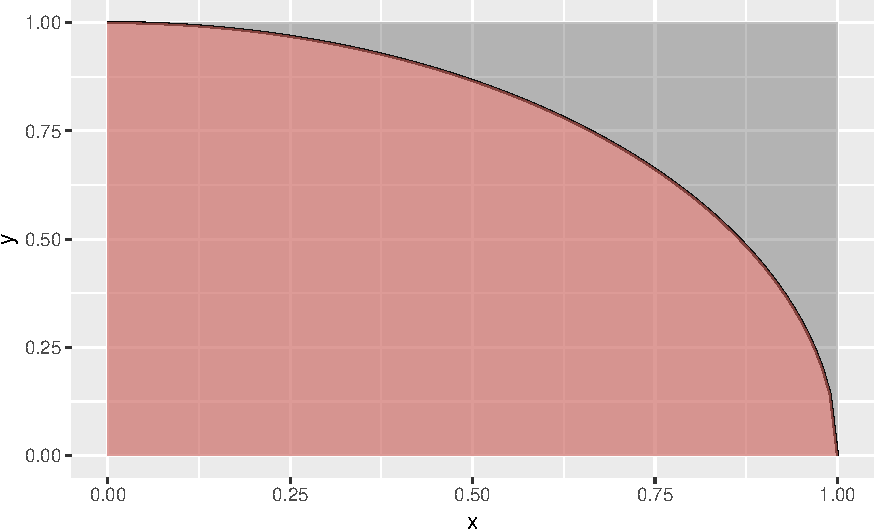
\includegraphics[width=0.7\linewidth]{statistical-computing_files/figure-latex/hmmc-1} 

}

\caption{Hit-or-Miss}\label{fig:hmmc}
\end{figure}

See Figure \ref{fig:hmmc}. From each coordinate, generate

\begin{itemize}
\tightlist
\item
  \(X_i \stackrel{iid}{\sim}unif(0,1)\)
\item
  \(Y_i \stackrel{iid}{\sim}unif(0,1)\)
\end{itemize}

Then the proportion of \(Y_i \le \sqrt{1 - X_i^2}\) estimates \(\frac{\pi}{4}\).

\begin{Shaded}
\begin{Highlighting}[]
\KeywordTok{tibble}\NormalTok{(}\DataTypeTok{x =} \KeywordTok{runif}\NormalTok{(}\DecValTok{10000}\NormalTok{), }\DataTypeTok{y =} \KeywordTok{runif}\NormalTok{(}\DecValTok{10000}\NormalTok{)) }\OperatorTok\StringTok{ }
\StringTok{  }\KeywordTok{summarise}\NormalTok{(}\DataTypeTok{hitormiss =} \KeywordTok{mean}\NormalTok{(y }\OperatorTok{<=}\StringTok{ }\KeywordTok{sqrt}\NormalTok{(}\DecValTok{1} \OperatorTok{-}\StringTok{ }\NormalTok{x}\OperatorTok{^}\DecValTok{2}\NormalTok{)) }\OperatorTok{*}\StringTok{ }\DecValTok{4}\NormalTok{)}
\CommentTok{#> # A tibble: 1 x 1}
\CommentTok{#>   hitormiss}
\CommentTok{#>       <dbl>}
\CommentTok{#> 1      3.15}
\end{Highlighting}
\end{Shaded}

\hypertarget{variance-and-efficiency}{%
\section{Variance and Efficiency}\label{variance-and-efficiency}}

We have seen two apporoaches doing the same task. Now we want to \emph{evaluate them}. Denote that simple Monte Carlo integration \ref{thm:mcint} is estimating the \emph{expected value of some random variable}. Proportion, which approximates probability is expected value of identity function.

The common statistic that can evaluate estimators expected value might be their variances.

\hypertarget{variance}{%
\subsection{Variance}\label{variance}}

Note that variance of sample mean is \(Var(\overline{g(X)}) = \frac{Var(g(X))}{N}\). This property is one of estimating variance of \(\hat\theta\).

\begin{equation}
  \widehat{Var}(\hat\theta) = \frac{1}{N}\bigg( \frac{1}{N} \sum_{i = 1}^N (g(X_i) - \overline{g(X_i)}) \bigg) = \frac{1}{N^2} \sum_{i = 1}^N (g(X_i) - \overline{g(X_i)})
  \label{eq:mcsamvar}
\end{equation}

For example,

\begin{Shaded}
\begin{Highlighting}[]
\KeywordTok{tibble}\NormalTok{(}\DataTypeTok{x =} \KeywordTok{runif}\NormalTok{(}\DecValTok{10000}\NormalTok{)) }\OperatorTok\StringTok{ }
\StringTok{  }\KeywordTok{summarise}\NormalTok{(}\DataTypeTok{mc_pi =} \KeywordTok{var}\NormalTok{(}\KeywordTok{circ}\NormalTok{(x)) }\OperatorTok{/}\StringTok{ }\DecValTok{10000}\NormalTok{)}
\CommentTok{#> # A tibble: 1 x 1}
\CommentTok{#>       mc_pi}
\CommentTok{#>       <dbl>}
\CommentTok{#> 1 0.0000795}
\end{Highlighting}
\end{Shaded}

However, this \emph{variance of sample mean} is used in situation when we are in sample limitation situation. We do not have to stick to this. Now, Generating samples as many as we want is possible. So we try another approach: \emph{parametric bootstrap}.

\begin{figure}[H]

{\centering 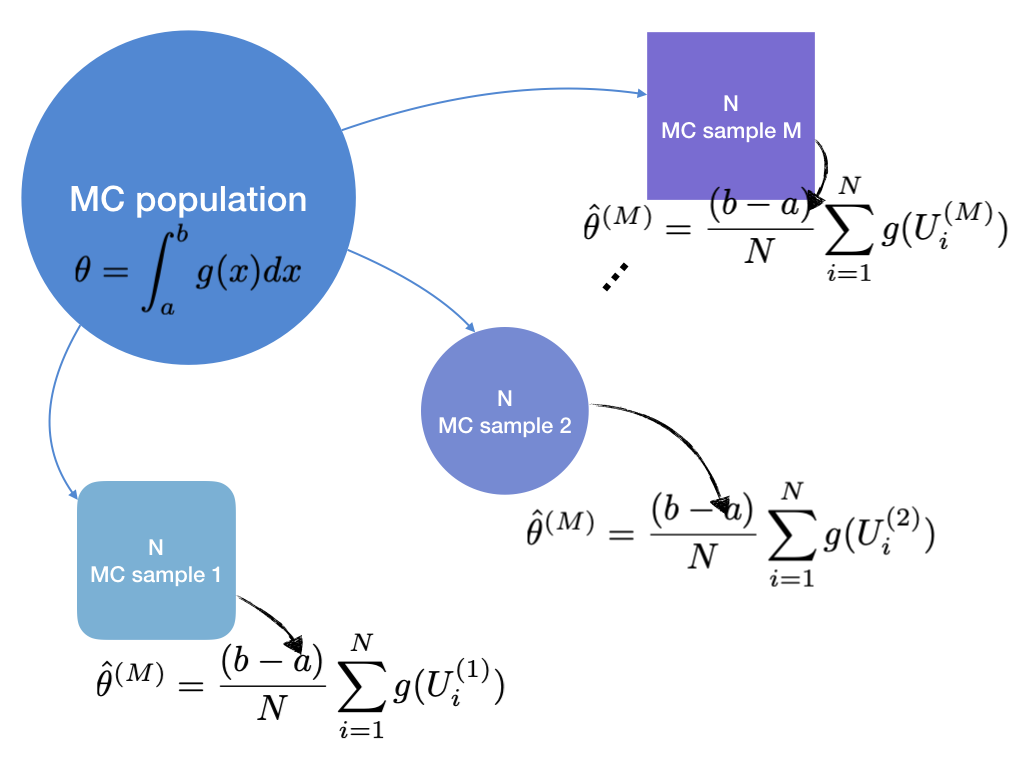
\includegraphics[width=0.7\linewidth]{images/mcint} 

}

\caption{Empircal distribution of $\hat\theta$}\label{fig:mcintvar}
\end{figure}

See Figure \ref{fig:mcintvar}. If we estimate \(E\Big[g(U \sim unif(a, b))\Big]\), we can get \(\theta\). Generate \(M\) samples \(\{ U_1^{(j)}, \ldots, U_N^{(j)} \}, j = 1, \ldots M\) from this \(U \sim unif(a, b)\). In each sample, calculate MC estimates \(\hat\theta^{(j)}\). Now we have \(M\) MC estimates \(\hat\theta\). This gives empirical distribution of \(\hat\theta\). By \emph{drawing a histogram}, we can see the outline.

\begin{algorithm}[H] \label{alg:algmcint}
  \SetAlgoLined
  \SetKwInOut{Input}{input}
  \SetKwInOut{Output}{output}
  \Input{$\theta = \int_a^b g(x) dx$}
  \For{$m \leftarrow 1$ \KwTo $M$}{
    Generate $U_1^{(m)}, \ldots, U_N^{(m)} \stackrel{iid}{\sim}unif(a, b)$ \;
    Compute $\hat\theta^{(j)} = \frac{(b - a)}{N} \sum g(U_i^{(j)})$\;
  }
  $\bar{\hat\theta} = \frac{1}{M} \sum \hat\theta^{(j)}$\;
  $\widehat{Var}(\hat\theta) = \frac{1}{M - 1} \sum (\hat\theta^{(j)} - \bar{\hat\theta})^2$\;
  \Output{$\widehat{Var}(\hat\theta)$}
  \caption{Variance of $\hat\theta$}
\end{algorithm}

Since we have to generate large size of data, \texttt{data.table} package will be used.

\begin{Shaded}
\begin{Highlighting}[]
\KeywordTok{library}\NormalTok{(data.table)}
\end{Highlighting}
\end{Shaded}

Group operation can be used. Additional column (\texttt{sam}) would indicate group, and for each group MC operation would be processed. The following is the function generating \texttt{data.table} before group operation.

\begin{Shaded}
\begin{Highlighting}[]
\NormalTok{mc_data <-}\StringTok{ }\ControlFlowTok{function}\NormalTok{(rand, }\DataTypeTok{N =} \DecValTok{10000}\NormalTok{, }\DataTypeTok{M =} \DecValTok{1000}\NormalTok{, }\DataTypeTok{char =} \StringTok{"s"}\NormalTok{, ...) \{}
  \KeywordTok{data.table}\NormalTok{(}
    \DataTypeTok{u =} \KeywordTok{rand}\NormalTok{(}\DataTypeTok{n =}\NormalTok{ N }\OperatorTok{*}\StringTok{ }\NormalTok{M, ...),}
    \DataTypeTok{sam =} \KeywordTok{gl}\NormalTok{(M, N, }\DataTypeTok{labels =} \KeywordTok{paste0}\NormalTok{(}\StringTok{"s"}\NormalTok{, }\DecValTok{1}\OperatorTok{:}\NormalTok{M))}
\NormalTok{  )}
\NormalTok{\}}
\end{Highlighting}
\end{Shaded}

\begin{Shaded}
\begin{Highlighting}[]
\NormalTok{pi_mc <-}
\StringTok{  }\KeywordTok{mc_data}\NormalTok{(runif)[,}
\NormalTok{                 .(}\DataTypeTok{mc_pi =} \KeywordTok{mean}\NormalTok{(}\KeywordTok{circ}\NormalTok{(u))),}
\NormalTok{                 keyby =}\StringTok{ }\NormalTok{sam]}
\end{Highlighting}
\end{Shaded}

\begin{Shaded}
\begin{Highlighting}[]
\NormalTok{pi_mc }\OperatorTok\StringTok{ }
\StringTok{  }\KeywordTok{ggplot}\NormalTok{(}\KeywordTok{aes}\NormalTok{(}\DataTypeTok{x =}\NormalTok{ mc_pi)) }\OperatorTok{+}
\StringTok{  }\KeywordTok{geom_histogram}\NormalTok{(}\DataTypeTok{bins =} \DecValTok{30}\NormalTok{, }\DataTypeTok{col =} \KeywordTok{gg_hcl}\NormalTok{(}\DecValTok{1}\NormalTok{), }\DataTypeTok{alpha =} \FloatTok{.7}\NormalTok{) }\OperatorTok{+}
\StringTok{  }\KeywordTok{xlab}\NormalTok{(}\KeywordTok{expression}\NormalTok{(pi)) }\OperatorTok{+}
\StringTok{  }\KeywordTok{geom_vline}\NormalTok{(}\DataTypeTok{xintercept =}\NormalTok{ pi, }\DataTypeTok{col =} \KeywordTok{gg_hcl}\NormalTok{(}\DecValTok{2}\NormalTok{)[}\DecValTok{2}\NormalTok{])}
\end{Highlighting}
\end{Shaded}

\begin{figure}[H]

{\centering 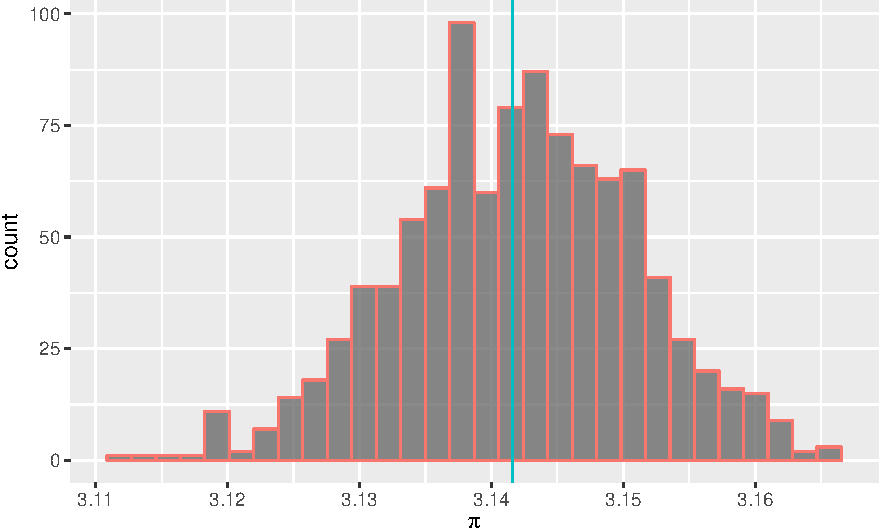
\includegraphics[width=0.7\linewidth]{statistical-computing_files/figure-latex/smchis-1} 

}

\caption{Empirical distribution of $\hat\pi$ by simple MC}\label{fig:smchis}
\end{figure}

As in Algorighm \(\ref{alg:algmcint}\), we can compute the variance as below.

\begin{Shaded}
\begin{Highlighting}[]
\NormalTok{(mc_var <-}
\StringTok{  }\NormalTok{pi_mc[,}
\NormalTok{        .(}\DataTypeTok{mc_variance =} \KeywordTok{var}\NormalTok{(mc_pi))])}
\CommentTok{#>    mc_variance}
\CommentTok{#> 1:    8.09e-05}
\end{Highlighting}
\end{Shaded}

On the other hand, we need to generate two sets of random numbers for hit-or-miss MC.

\begin{Shaded}
\begin{Highlighting}[]
\NormalTok{pi_hit <-}
\StringTok{  }\KeywordTok{mc_data}\NormalTok{(runif)[}
\NormalTok{    , u2 }\OperatorTok{:}\ErrorTok{=}\StringTok{ }\KeywordTok{runif}\NormalTok{(}\DecValTok{10000} \OperatorTok{*}\StringTok{ }\DecValTok{1000}\NormalTok{)}
\NormalTok{  ][,}
\NormalTok{    .(}\DataTypeTok{hitormiss =} \KeywordTok{mean}\NormalTok{(u2 }\OperatorTok{<=}\StringTok{ }\KeywordTok{sqrt}\NormalTok{(}\DecValTok{1} \OperatorTok{-}\StringTok{ }\NormalTok{u}\OperatorTok{^}\DecValTok{2}\NormalTok{)) }\OperatorTok{*}\StringTok{ }\DecValTok{4}\NormalTok{),}
\NormalTok{    keyby =}\StringTok{ }\NormalTok{sam]}
\end{Highlighting}
\end{Shaded}

\begin{Shaded}
\begin{Highlighting}[]
\NormalTok{pi_mc[pi_hit] }\OperatorTok\StringTok{ }
\StringTok{  }\KeywordTok{melt}\NormalTok{(}\DataTypeTok{id.vars =} \StringTok{"sam"}\NormalTok{, }\DataTypeTok{variable.name =} \StringTok{"hat"}\NormalTok{) }\OperatorTok\StringTok{ }
\StringTok{  }\KeywordTok{ggplot}\NormalTok{(}\KeywordTok{aes}\NormalTok{(}\DataTypeTok{x =}\NormalTok{ value, }\DataTypeTok{fill =}\NormalTok{ hat)) }\OperatorTok{+}
\StringTok{  }\KeywordTok{geom_histogram}\NormalTok{(}\DataTypeTok{bins =} \DecValTok{30}\NormalTok{, }\DataTypeTok{alpha =} \FloatTok{.5}\NormalTok{, }\DataTypeTok{position =} \StringTok{"identity"}\NormalTok{) }\OperatorTok{+}
\StringTok{  }\KeywordTok{xlab}\NormalTok{(}\KeywordTok{expression}\NormalTok{(pi)) }\OperatorTok{+}
\StringTok{  }\KeywordTok{geom_vline}\NormalTok{(}\DataTypeTok{xintercept =}\NormalTok{ pi, }\DataTypeTok{col =} \KeywordTok{I}\NormalTok{(}\StringTok{"red"}\NormalTok{)) }\OperatorTok{+}
\StringTok{  }\KeywordTok{scale_fill_discrete}\NormalTok{(}
    \DataTypeTok{name =} \StringTok{"MC"}\NormalTok{,}
    \DataTypeTok{labels =} \KeywordTok{c}\NormalTok{(}\StringTok{"Simple"}\NormalTok{, }\StringTok{"Hit-or-Miss"}\NormalTok{)}
\NormalTok{  )}
\end{Highlighting}
\end{Shaded}

\begin{figure}[H]

{\centering 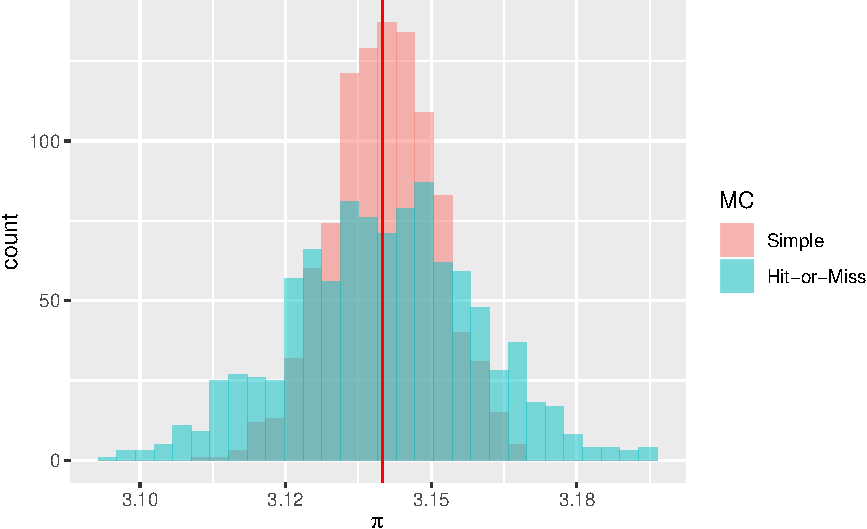
\includegraphics[width=0.7\linewidth]{statistical-computing_files/figure-latex/simhit-1} 

}

\caption{Simple MC and Hit-or-Miss MC}\label{fig:simhit}
\end{figure}

\begin{Shaded}
\begin{Highlighting}[]
\NormalTok{(hit_var <-}
\StringTok{  }\NormalTok{pi_hit[,}
\NormalTok{         .(}\DataTypeTok{hit_variance =} \KeywordTok{var}\NormalTok{(hitormiss))])}
\CommentTok{#>    hit_variance}
\CommentTok{#> 1:     0.000258}
\end{Highlighting}
\end{Shaded}

\hypertarget{efficiency-1}{%
\subsection{Efficiency}\label{efficiency-1}}

See Figure \ref{fig:simhit}. It is obvious that Hit-or-Miss estimate produces larger variance than simple MC.

\BeginKnitrBlock{definition}[Efficiency]
\protect\hypertarget{def:eff}{}{\label{def:eff} \iffalse (Efficiency) \fi{} }Let \(\hat\theta_1\) and \(\hat\theta_2\) be two estimators for \(\theta\). Then \(\hat\theta_1\) is more efficient than \(\hat\theta_2\) if

\[\frac{Var(\hat\theta_1)}{Var(\hat\theta_2)} < 1\]
\EndKnitrBlock{definition}

In other words, if \(\hat\theta_1\) has smaller variance than \(\hat\theta_2\), then \(\hat\theta_1\) is said to be efficient, which is preferable.

\begin{longtable}{r|r|l}
\caption{\label{tab:unnamed-chunk-50}Simple MC versus Hit-or-Miss}\\
\hline
SimpleMC & Hit-or-Miss & SimpleMCefficiency\\
\hline
0 & 0 & TRUE\\
\hline
\end{longtable}

\hypertarget{variance-reduction}{%
\section{Variance Reduction}\label{variance-reduction}}

Consider Equation \eqref{eq:mcsamvar} based on \(Var(\hat\theta) = \frac{\sigma^2}{N}\). This variance can always reduced by adding \(N\). But we want to reduce variance less computationally.

\hypertarget{antithetic-variables}{%
\subsection{Antithetic Variables}\label{antithetic-variables}}

Consider correlated random variables \(U_1\) and \(U_2\). Then we have

\[Var\bigg( \frac{U_1 + U_2}{2} \bigg) = \frac{1}{4}\Big( Var(U_1) +  Var(U_2) + 2Cov(U_1, U_2)\Big)\]

See the last term \(Cov(U_1, U_2)\). If we generate \(U_{i1}\) and \(U_{i2}\) negatively correlated, we can get reduced variance than previous i.i.d. sample

\[Var\bigg( \frac{U_1 + U_2}{2} \bigg) = \frac{1}{4}\Big( Var(U_1) +  Var(U_2)\Big)\]

\BeginKnitrBlock{lemma}
\protect\hypertarget{lem:antiunif}{}{\label{lem:antiunif} }\(U\) and \(1 - U\) are identically distributed, but \emph{negatively correlated}.

\begin{enumerate}
  \item $U \sim unif(0,1) \Leftrightarrow 1 - U \sim unif(0,1)$
  \item $Corr(U, 1 - U) = -1$
\end{enumerate}
\EndKnitrBlock{lemma}

This is well-known property of uniform distribution. Instead of generating \(N\) uniform numbers, try \(\frac{N}{2}\) \(U_i\) and make corresponding \(\frac{N}{2}\) \(1 - U_i\). This sequence becomes negatively correlated, so we can reduce the variance as mentioned.

When can we replace previous numbers with these \emph{antithetic variables}? We usually plug-in the numbers in some function \(h\) to get Monte carlo integration. The thing is, our target is \(h\), not \(U\). \(h(U)\) and \(h(1 - U)\) should \emph{still be negatively correlated}. Hence, \(h\) should be \emph{monotonic function}.

\BeginKnitrBlock{corollary}
\protect\hypertarget{cor:antifun}{}{\label{cor:antifun} }If \(g = g(X_1, \ldots, X_n)\) is monotone, then

\[Y = g(F_X^{-1}(U_1), \ldots, F_X^{-1}(U_n))\]

and

\[Y^{\prime} = g(F_X^{-1}(1 - U_1), \ldots, F_X^{-1}(1 - U_n))\]

are negatively correlated.
\EndKnitrBlock{corollary}

\begin{algorithm}[H] \label{alg:alganti}
  \SetAlgoLined
  \SetKwInOut{Input}{input}
  \SetKwInOut{Output}{output}
  \Input{$h: monotonic$}
  \For{$m \leftarrow 1$ \KwTo $M$}{
    Generate $U_{1,1}^{(m)}, \ldots, U_{\frac{N}{2},1}^{(m)} \stackrel{iid}{\sim}unif(0, 1)$\;
    Set $U_{i,2}^{(m)} := 1 - U_{i,1}^{(m)} \stackrel{iid}{\sim}unif(0, 1)$\;
    $\{U_{i}^{(m)}\}_1^N = \{ U_{1,1}^{(m)}, \ldots, U_{{\frac{N}{2}},2}^{(m)} \}$\;
    $\hat\theta^{(j)} = \frac{1}{N} \sum h(U_i^{(j)})$\;
  }
  $\bar{\hat\theta} = \frac{1}{M} \sum \hat\theta^{(j)}$\;
  $\widehat{Var}(\hat\theta) = \frac{1}{M - 1} \sum (\hat\theta^{(j)} - \bar{\hat\theta})^2$\;
  \Output{$\widehat{Var}(\hat\theta)$}
  \caption{Variance of $\hat\theta$ using antithetic variables}
\end{algorithm}

Check again Example \ref{exm:mcex}. We have try to calculate

\[\Phi(x) = \int_{-\infty}^x \frac{1}{\sqrt{2\pi}}\exp\bigg(-\frac{t^2}{2}\bigg)dt\]

using simple monte carlo. To make the support \((0, 1)\), let \(y = \frac{t}{x}\) be a change of variable. Then

\begin{equation*}
  \begin{split}
    \int_0^x \exp\bigg(-\frac{t^2}{2}\bigg) dt & = \int_0^1 x\exp\bigg(-\frac{(xy)^2}{2}\bigg) dy \\
    & \approx \frac{1}{N} \sum_{i = 1}^N x\exp\bigg(-\frac{(xU_i)^2}{2}\bigg)
  \end{split}
\end{equation*}

\begin{Shaded}
\begin{Highlighting}[]
\NormalTok{phiunif <-}\StringTok{ }\ControlFlowTok{function}\NormalTok{(x, y) \{}
\NormalTok{  yi <-}\StringTok{ }\KeywordTok{abs}\NormalTok{(y)}
\NormalTok{  theta <-}\StringTok{ }\KeywordTok{mean}\NormalTok{(yi }\OperatorTok{*}\StringTok{ }\KeywordTok{exp}\NormalTok{(}\OperatorTok{-}\NormalTok{(yi }\OperatorTok{*}\StringTok{ }\NormalTok{x)}\OperatorTok{^}\DecValTok{2} \OperatorTok{/}\StringTok{ }\DecValTok{2}\NormalTok{)) }\OperatorTok{/}\StringTok{ }\KeywordTok{sqrt}\NormalTok{(}\DecValTok{2} \OperatorTok{*}\StringTok{ }\NormalTok{pi) }\OperatorTok{+}\StringTok{ }\FloatTok{.5}
  \KeywordTok{ifelse}\NormalTok{(y }\OperatorTok{>=}\StringTok{ }\DecValTok{0}\NormalTok{, theta, }\DecValTok{1} \OperatorTok{-}\StringTok{ }\NormalTok{theta)}
\NormalTok{\}}
\end{Highlighting}
\end{Shaded}

Consider \(\Phi(2)\).

\begin{Shaded}
\begin{Highlighting}[]
\NormalTok{phi2 <-}
\StringTok{  }\KeywordTok{mc_data}\NormalTok{(runif)[,}
\NormalTok{                 .(}\DataTypeTok{p2 =} \KeywordTok{phiunif}\NormalTok{(u, }\DataTypeTok{y =} \DecValTok{2}\NormalTok{)),}
\NormalTok{                 keyby =}\StringTok{ }\NormalTok{sam]}
\end{Highlighting}
\end{Shaded}

Now apply antithetic variables.

\begin{Shaded}
\begin{Highlighting}[]
\NormalTok{phi2_anti <-}
\StringTok{  }\KeywordTok{mc_data}\NormalTok{(runif, }\DataTypeTok{N =} \DecValTok{10000} \OperatorTok{/}\StringTok{ }\DecValTok{2}\NormalTok{)[,}
\NormalTok{                                u2 }\OperatorTok{:}\ErrorTok{=}\StringTok{ }\DecValTok{1} \OperatorTok{-}\StringTok{ }\NormalTok{u] }\OperatorTok\StringTok{ }
\StringTok{  }\KeywordTok{melt}\NormalTok{(}\DataTypeTok{id.vars =} \StringTok{"sam"}\NormalTok{, }\DataTypeTok{value.name =} \StringTok{"U"}\NormalTok{) }\OperatorTok\StringTok{ }
\StringTok{  }\NormalTok{.[,}
\NormalTok{    .(}\DataTypeTok{anti_p2 =} \KeywordTok{phiunif}\NormalTok{(U, }\DataTypeTok{y =} \DecValTok{2}\NormalTok{)),}
\NormalTok{    keyby =}\StringTok{ }\NormalTok{sam]}
\end{Highlighting}
\end{Shaded}

\begin{Shaded}
\begin{Highlighting}[]
\NormalTok{phi2[phi2_anti] }\OperatorTok\StringTok{ }
\StringTok{  }\KeywordTok{melt}\NormalTok{(}\DataTypeTok{id.vars =} \StringTok{"sam"}\NormalTok{, }\DataTypeTok{variable.name =} \StringTok{"hat"}\NormalTok{) }\OperatorTok\StringTok{ }
\StringTok{  }\KeywordTok{ggplot}\NormalTok{(}\KeywordTok{aes}\NormalTok{(}\DataTypeTok{x =}\NormalTok{ value, }\DataTypeTok{fill =}\NormalTok{ hat)) }\OperatorTok{+}
\StringTok{  }\KeywordTok{geom_histogram}\NormalTok{(}\DataTypeTok{bins =} \DecValTok{30}\NormalTok{, }\DataTypeTok{alpha =} \FloatTok{.5}\NormalTok{, }\DataTypeTok{position =} \StringTok{"identity"}\NormalTok{) }\OperatorTok{+}
\StringTok{  }\KeywordTok{xlab}\NormalTok{(}\KeywordTok{expression}\NormalTok{(pi)) }\OperatorTok{+}
\StringTok{  }\KeywordTok{geom_vline}\NormalTok{(}\DataTypeTok{xintercept =} \KeywordTok{pnorm}\NormalTok{(}\DecValTok{2}\NormalTok{), }\DataTypeTok{col =} \KeywordTok{I}\NormalTok{(}\StringTok{"red"}\NormalTok{)) }\OperatorTok{+}
\StringTok{  }\KeywordTok{scale_fill_discrete}\NormalTok{(}
    \DataTypeTok{name =} \StringTok{"MC"}\NormalTok{,}
    \DataTypeTok{labels =} \KeywordTok{c}\NormalTok{(}\StringTok{"Simple"}\NormalTok{, }\StringTok{"Antithetic"}\NormalTok{)}
\NormalTok{  )}
\end{Highlighting}
\end{Shaded}

\begin{figure}[H]

{\centering 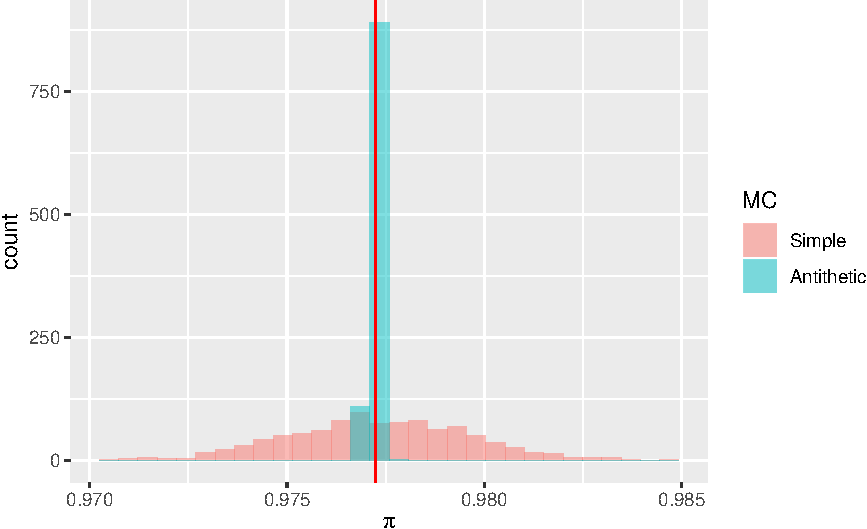
\includegraphics[width=0.7\linewidth]{statistical-computing_files/figure-latex/svsanti-1} 

}

\caption{Use of antithetic variables}\label{fig:svsanti}
\end{figure}

Obviously, variance has been reduced.

\begin{Shaded}
\begin{Highlighting}[]
\NormalTok{phi2[phi2_anti] }\OperatorTok\StringTok{ }
\StringTok{  }\KeywordTok{melt}\NormalTok{(}\DataTypeTok{id.vars =} \StringTok{"sam"}\NormalTok{, }\DataTypeTok{variable.name =} \StringTok{"hat"}\NormalTok{) }\OperatorTok\StringTok{ }
\StringTok{  }\NormalTok{.[,}
\NormalTok{    .(}\DataTypeTok{variance =} \KeywordTok{var}\NormalTok{(value)),}
\NormalTok{    by =}\StringTok{ }\NormalTok{hat]}
\CommentTok{#>        hat variance}
\CommentTok{#> 1:      p2  5.2e-06}
\CommentTok{#> 2: anti_p2  1.5e-08}
\end{Highlighting}
\end{Shaded}

\hypertarget{control-variates}{%
\subsection{Control Variates}\label{control-variates}}

Recall that we are trying to estimate \(\theta = Eg(X)\) here in MC integration. Consider other output random variable. Suppose that \(\mu_f \equiv Ef(Y)\) is known. It is obvious that

\begin{equation}
  \hat\theta_c = g(X) + c\Big(f(Y) - \mu_f\Big)
  \label{eq:controlest}
\end{equation}

is an unbiased estimator for \(\theta\) for any \(c \in \mathbb{R}\). Then we have

\begin{equation}
  Var\hat\theta_c = Varg(X) + c^2 Varf(X) + 2cCov(g(X), f(X))
  \label{eq:controlvar}
\end{equation}

Recall that our goal is to minimize this \(Var\hat\theta_c\). What value of \(c\) is to be determined? Note that Equation \eqref{eq:controlvar} is quadratic function of \(c\).

\begin{equation}
  \begin{split}
    Var\hat\theta_c & = Varf(X) c^2 + 2cCov(g(X), f(X)) + Varg(X) \\
    & = Var f(X) \bigg( c + \frac{Cov(g(X), f(X))}{Var f(X)} \bigg)^2 + Var g(X) - \frac{Cov(g(X), f(X))^2}{Var f(X)}
  \end{split}
  \label{eq:controlc}
\end{equation}

From Equation \eqref{eq:controlc}, the variance is minimized at

\begin{equation}
  c^{\ast} = - \frac{Cov(g(X), f(X))}{Var f(X)}
  \label{eq:controlsol}
\end{equation}

with minimum variance

\[Var\hat\theta_{c^{\ast}} = Var g(X) - \frac{Cov(g(X), f(X))^2}{Var f(X)}\]

By this, we can reduce the variance of estimation as much as possible (using \(f(X)\)). Here, \(f(X)\) is called a \emph{control variate} for \(g(X)\).

\begin{algorithm}[H] \label{alg:algcontrol}
  \SetAlgoLined
  \SetKwInOut{Input}{input}
  \SetKwInOut{Output}{output}
  \Input{$g$, control variate $f$ with mean $\mu_f$}
  \For{$m \leftarrow 1$ \KwTo $M$}{
    Generate $U_1^{(m)}, \ldots, U_N^{(m)} \stackrel{iid}{\sim}unif$\;
    Set $g = g(U_i)$ and $f = f(U_i)$\;
    Compute $\hat{c}^{\ast(m)} = - \frac{\widehat{Cov}(g, f)}{\widehat{Var}(f)}$\;
    $\hat\theta_{c^{\ast}}^{(j)} = g + c^{\ast(m)}(f - \mu_f)$\;
  }
  $\bar{\hat\theta} = \frac{1}{M} \sum \hat\theta_{c^{\ast}}^{(j)}$\;
  $\widehat{Var}(\hat\theta) = \frac{1}{M - 1} \sum (\hat\theta_{c^{\ast}}^{(j)} - \bar{\hat\theta})^2$\;
  \Output{$\widehat{Var}(\hat\theta)$}
  \caption{Variance of $\hat\theta$ using control variables}
\end{algorithm}

\BeginKnitrBlock{example}[Variance reduction by control variate]
\protect\hypertarget{exm:intex}{}{\label{exm:intex} \iffalse (Variance reduction by control variate) \fi{} }Apply each simple MC, antithtic variate, and control variate to

\[\int_0^1 e^x dx\]
\EndKnitrBlock{example}

\begin{Shaded}
\begin{Highlighting}[]
\NormalTok{N <-}\StringTok{ }\DecValTok{100}
\NormalTok{M <-}\StringTok{ }\DecValTok{1000}
\end{Highlighting}
\end{Shaded}

Denote that the true value is

\[\int_0^1 e^x dx = e - 1 = 1.718\]

We might compare each estimate to this.

\BeginKnitrBlock{solution}[Simple MC]
\iffalse{} {Solution (Simple MC). } \fi{}We only need \(U \sim unif(0, 1)\).

\begin{equation}
  \begin{split}
    \theta & = \int_0^1 e^x dx \\
    & = \int_0^1 e^x I_{(0,1)}(x)dx \\
    & \approx \frac{1}{N} \sum_{i = 1}^N e^{u_i}, \qquad u_i \stackrel{iid}{\sim}unif(0, 1)
  \end{split}
  \label{eq:mcsol}
\end{equation}
\EndKnitrBlock{solution}

\begin{Shaded}
\begin{Highlighting}[]
\NormalTok{theta_sim <-}
\StringTok{  }\KeywordTok{mc_data}\NormalTok{(runif, }\DataTypeTok{N =}\NormalTok{ N, }\DataTypeTok{M =}\NormalTok{ M)[,}
\NormalTok{                               .(}\DataTypeTok{mc =} \KeywordTok{mean}\NormalTok{(}\KeywordTok{exp}\NormalTok{(u))),}
\NormalTok{                               keyby =}\StringTok{ }\NormalTok{sam]}
\end{Highlighting}
\end{Shaded}

\begin{verbatim}
#>         sam   mc
#>    1:    s1 1.70
#>    2:    s2 1.71
#>    3:    s3 1.76
#>    4:    s4 1.71
#>    5:    s5 1.73
#>   ---           
#>  996:  s996 1.79
#>  997:  s997 1.82
#>  998:  s998 1.68
#>  999:  s999 1.73
#> 1000: s1000 1.76
\end{verbatim}

\BeginKnitrBlock{solution}[Antithetic variate]
\iffalse{} {Solution (Antithetic variate). } \fi{}For \(N^{\prime} = \frac{N}{2}\),

Consider \(u_1, \ldots, u_{N^{\prime}} \stackrel{iid}{\sim}unif(0,1)\) and \(1 - u_{1}, \ldots, 1 - u_{N^{\prime}} \stackrel{iid}{\sim}unif(0,1)\).

See Equation \eqref{eq:mcsol}. Then we can compute antithetic estimator by

\begin{equation*}
  \begin{split}
    \hat\theta_A & = \frac{1}{N} \sum_{i = 1}^{N / 2} \Big( e^{u_i} + e^{1 - u_i} \Big) \\
    & = \frac{1}{N / 2} \sum_{i = 1}^{N / 2} \bigg( \frac{e^{u_i} + e^{1 - u_i}}{2} \bigg) \\
    & = \text{sample mean}
  \end{split}
\end{equation*}
\EndKnitrBlock{solution}

\begin{Shaded}
\begin{Highlighting}[]
\NormalTok{theta_anti <-}
\StringTok{  }\KeywordTok{mc_data}\NormalTok{(runif, }\DataTypeTok{N =}\NormalTok{ N }\OperatorTok{/}\StringTok{ }\DecValTok{2}\NormalTok{, }\DataTypeTok{M =}\NormalTok{ M)[,}
\NormalTok{                                   u2 }\OperatorTok{:}\ErrorTok{=}\StringTok{ }\DecValTok{1} \OperatorTok{-}\StringTok{ }\NormalTok{u][,}
\NormalTok{                                                .(}\DataTypeTok{anti =} \KeywordTok{mean}\NormalTok{((}\KeywordTok{exp}\NormalTok{(u) }\OperatorTok{+}\StringTok{ }\KeywordTok{exp}\NormalTok{(u2)) }\OperatorTok{/}\StringTok{ }\DecValTok{2}\NormalTok{)),}
\NormalTok{                                                keyby =}\StringTok{ }\NormalTok{sam]}
\end{Highlighting}
\end{Shaded}

Now look at the results of the two.

\begin{Shaded}
\begin{Highlighting}[]
\NormalTok{theta_sim[theta_anti] }\OperatorTok\StringTok{ }
\StringTok{  }\KeywordTok{melt}\NormalTok{(}\DataTypeTok{id.vars =} \StringTok{"sam"}\NormalTok{, }\DataTypeTok{variable.name =} \StringTok{"simul"}\NormalTok{, }\DataTypeTok{value.name =} \StringTok{"integral"}\NormalTok{) }\OperatorTok\StringTok{ }
\StringTok{  }\KeywordTok{ggplot}\NormalTok{(}\KeywordTok{aes}\NormalTok{(}\DataTypeTok{x =}\NormalTok{ integral, }\DataTypeTok{fill =}\NormalTok{ simul)) }\OperatorTok{+}
\StringTok{  }\KeywordTok{geom_histogram}\NormalTok{(}\DataTypeTok{bins =} \DecValTok{30}\NormalTok{, }\DataTypeTok{position =} \StringTok{"identity"}\NormalTok{, }\DataTypeTok{alpha =} \FloatTok{.5}\NormalTok{) }\OperatorTok{+}
\StringTok{  }\KeywordTok{xlab}\NormalTok{(}\KeywordTok{expression}\NormalTok{(theta)) }\OperatorTok{+}
\StringTok{  }\KeywordTok{geom_vline}\NormalTok{(}\DataTypeTok{xintercept =} \KeywordTok{exp}\NormalTok{(}\DecValTok{1}\NormalTok{) }\OperatorTok{-}\StringTok{ }\DecValTok{1}\NormalTok{, }\DataTypeTok{col =} \KeywordTok{I}\NormalTok{(}\StringTok{"red"}\NormalTok{)) }\OperatorTok{+}
\StringTok{  }\KeywordTok{scale_fill_discrete}\NormalTok{(}
    \DataTypeTok{name =} \StringTok{"MC"}\NormalTok{,}
    \DataTypeTok{labels =} \KeywordTok{c}\NormalTok{(}\StringTok{"Simple"}\NormalTok{, }\StringTok{"Antithetic"}\NormalTok{)}
\NormalTok{  )}
\end{Highlighting}
\end{Shaded}

\begin{figure}[H]

{\centering 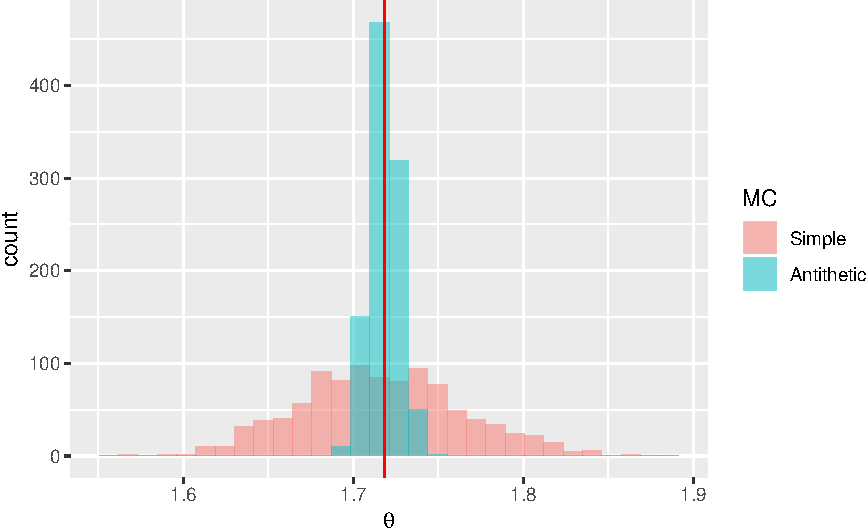
\includegraphics[width=0.7\linewidth]{statistical-computing_files/figure-latex/compantihat-1} 

}

\caption{Antithetic variate estimator}\label{fig:compantihat}
\end{figure}

It is clear that antithetic variate have reduced variance.

\BeginKnitrBlock{solution}[Control variate]
\iffalse{} {Solution (Control variate). } \fi{}Consider

\[g(U) = e^U\]

and

\[f(U) = U\]

with \(U \sim unif(0, 1)\).

Note that

\[E(U) = \frac{1}{2}\]

Then

\[\hat\theta_C = e^U + c\bigg(U - \frac{1}{2}\bigg)\]

is an unbiased estimator of \(\theta = \int_0^1 e^xdx\).

To reduce variance, we need to set \(c\) to be

\[c^{\ast} = -\frac{Cov(e^U, U)}{Var(U)}\]
\EndKnitrBlock{solution}

Since we do not know the exact number, we estimate this from each Monte Carlo sample.

\begin{Shaded}
\begin{Highlighting}[]
\NormalTok{theta_con <-}
\StringTok{  }\KeywordTok{mc_data}\NormalTok{(runif, }\DataTypeTok{N =}\NormalTok{ N, }\DataTypeTok{M =}\NormalTok{ M)[,}
\NormalTok{                               chat }\OperatorTok{:}\ErrorTok{=}\StringTok{ }\OperatorTok{-}\StringTok{ }\KeywordTok{cov}\NormalTok{(}\KeywordTok{exp}\NormalTok{(u), u) }\OperatorTok{/}\StringTok{ }\KeywordTok{var}\NormalTok{(u),}
\NormalTok{                               by =}\StringTok{ }\NormalTok{sam][,}
\NormalTok{                                         .(}\DataTypeTok{con =} \KeywordTok{mean}\NormalTok{(}\KeywordTok{exp}\NormalTok{(u) }\OperatorTok{+}\StringTok{ }\NormalTok{chat }\OperatorTok{*}\StringTok{ }\NormalTok{(u }\OperatorTok{-}\StringTok{ }\DecValTok{1} \OperatorTok{/}\StringTok{ }\DecValTok{2}\NormalTok{))),}
\NormalTok{                                         keyby =}\StringTok{ }\NormalTok{sam]}
\end{Highlighting}
\end{Shaded}

\begin{Shaded}
\begin{Highlighting}[]
\NormalTok{thetahat <-}\StringTok{ }\NormalTok{theta_sim[theta_anti][theta_con]}
\end{Highlighting}
\end{Shaded}

\begin{Shaded}
\begin{Highlighting}[]
\NormalTok{thetahat }\OperatorTok\StringTok{ }
\StringTok{  }\KeywordTok{melt}\NormalTok{(}\DataTypeTok{id.vars =} \StringTok{"sam"}\NormalTok{, }\DataTypeTok{variable.name =} \StringTok{"simul"}\NormalTok{, }\DataTypeTok{value.name =} \StringTok{"integral"}\NormalTok{) }\OperatorTok\StringTok{ }
\StringTok{  }\KeywordTok{ggplot}\NormalTok{(}\KeywordTok{aes}\NormalTok{(}\DataTypeTok{x =}\NormalTok{ integral, }\DataTypeTok{fill =}\NormalTok{ simul)) }\OperatorTok{+}
\StringTok{  }\KeywordTok{geom_histogram}\NormalTok{(}\DataTypeTok{bins =} \DecValTok{30}\NormalTok{, }\DataTypeTok{position =} \StringTok{"identity"}\NormalTok{, }\DataTypeTok{alpha =} \FloatTok{.5}\NormalTok{) }\OperatorTok{+}
\StringTok{  }\KeywordTok{xlab}\NormalTok{(}\KeywordTok{expression}\NormalTok{(theta)) }\OperatorTok{+}
\StringTok{  }\KeywordTok{geom_vline}\NormalTok{(}\DataTypeTok{xintercept =} \KeywordTok{exp}\NormalTok{(}\DecValTok{1}\NormalTok{) }\OperatorTok{-}\StringTok{ }\DecValTok{1}\NormalTok{, }\DataTypeTok{col =} \KeywordTok{I}\NormalTok{(}\StringTok{"red"}\NormalTok{)) }\OperatorTok{+}
\StringTok{  }\KeywordTok{scale_fill_discrete}\NormalTok{(}
    \DataTypeTok{name =} \StringTok{"MC"}\NormalTok{,}
    \DataTypeTok{labels =} \KeywordTok{c}\NormalTok{(}\StringTok{"Simple"}\NormalTok{, }\StringTok{"Antithetic"}\NormalTok{, }\StringTok{"Control"}\NormalTok{)}
\NormalTok{  )}
\end{Highlighting}
\end{Shaded}

\begin{figure}[H]

{\centering 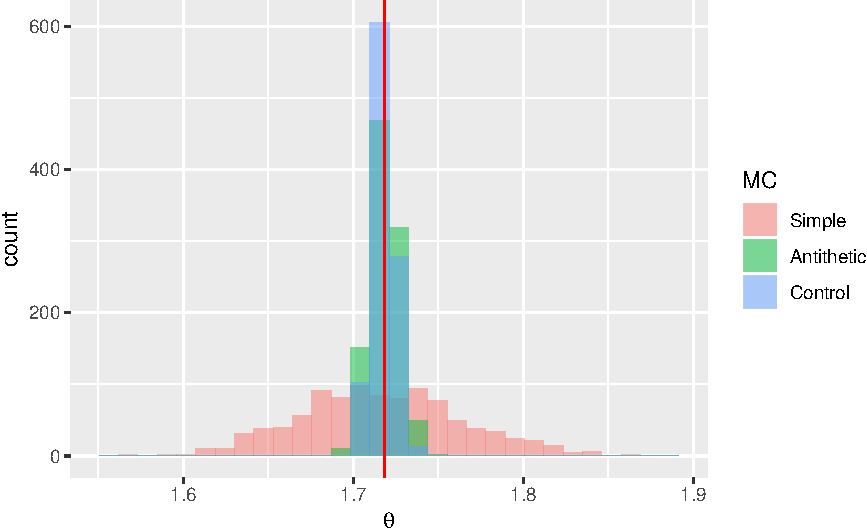
\includegraphics[width=0.7\linewidth]{statistical-computing_files/figure-latex/compcontrol-1} 

}

\caption{Use of Control variable}\label{fig:compcontrol}
\end{figure}

It looks like control variate have less variance, but what is more important is that both methods successfully have reduced it.

\begin{Shaded}
\begin{Highlighting}[]
\NormalTok{thetahat[,}
         \KeywordTok{lapply}\NormalTok{(.SD, sd),}
\NormalTok{         ,.SDcols =}\StringTok{ }\OperatorTok{-}\StringTok{"sam"}\NormalTok{]}
\CommentTok{#>       mc    anti     con}
\CommentTok{#> 1: 0.049 0.00872 0.00643}
\end{Highlighting}
\end{Shaded}

\hypertarget{antithetic-variate-as-control-variate}{%
\subsection{Antithetic variate as control variate}\label{antithetic-variate-as-control-variate}}

Both antithetic variate and control variate reduce variance using covariance between two random variables. Actually, \emph{antithetic variate is a special case of control variate}. See Equation \eqref{eq:controlest}.

\BeginKnitrBlock{lemma}
\protect\hypertarget{lem:unnamed-chunk-65}{}{\label{lem:unnamed-chunk-65} }Control variate estimator is a linear combination of unbiased estimators of \(\theta\).
\EndKnitrBlock{lemma}

Consider any two unbiased estimator \(\hat\theta_1\) and \(\hat\theta_2\) for \(\theta = Eg(X)\). Build control variate as following.

\[\hat\theta_c = c\hat\theta_1 + (1 - c)\hat\theta_2\]

It is obvious that \(\hat\theta_c\) is also unbiased of \(\theta\) for every \(c \in \mathbb{R}\).

\begin{equation}
  Var(\hat\theta_c) = Var(\hat\theta_2) + c^2 Var(\hat\theta_1 - \hat\theta_2) 2c Cov(\hat\theta_2, \hat\theta_1 - \hat\theta_2)
  \label{eq:controlvar2}
\end{equation}

Let \(\hat\theta_1\) and \(\hat\theta_2\) be antithetic variate choice. Recall that \emph{antithetic variate} give that for \(\hat\theta_1\) and \(\hat\theta_2\),

\[\hat\theta_1, \hat\theta_2 \sim IID, \quad Corr(\hat\theta_1, \hat\theta_2) = -1\]

It follows that

\[Cov(\hat\theta_1, \hat\theta_2) = - Var(\hat\theta_1)\]

and that

\[Var(\hat\theta_c) = (4c^2 - 4c + 1)Var(\hat\theta_1)\]

Hence, it leads to choosing optimal

\[\hat\theta_{c^{\ast}} = \frac{\hat\theta_1 + \hat\theta_2}{2}\]

which we have been used in antithetic variate.

\hypertarget{several-control-variates}{%
\subsection{Several control variates}\label{several-control-variates}}

To summarize, control variate try to reduce variance by combining unbiased estimatros of the target parameter. We have used one variate \(f(X)\). It might be possible to extend to multiple variates, so to speak, \(f_1(X), \ldots, f_k(X)\). Thanks to the linearity of expectation,

\[\hat\theta_c = g(X) + \sum_{i = 1}^k c_i \Big(f_i (X) - \mu_i\Big)\]

is also unbiased estimator, where \(\mu_i = E f_i(X)\). How to get each \(c_i^{\ast}\)? Rather than using variance and covariance, we can \emph{fitting linear regression}.

\hypertarget{control-variates-and-regression}{%
\subsection{Control variates and regression}\label{control-variates-and-regression}}

See Equation \eqref{eq:controlest} and Equation \eqref{eq:controlsol}. It can be found that we were estimating linear regression coefficient as LSE.

\BeginKnitrBlock{lemma}[Least squares estimator]
\protect\hypertarget{lem:lse}{}{\label{lem:lse} \iffalse (Least squares estimator) \fi{} }Consider \(Y_i = \beta_0 + \beta_1 X_i + \epsilon_i\). Then

\[\hat\beta_1 = \frac{\sum(X_i - \overline{X})(Y_i - \overline{Y})}{\sum (Y_i - \overline{Y})} = \frac{\widehat{Cov}(X, Y)}{\widehat{Var}(Y)}\]
\EndKnitrBlock{lemma}

Control variate estimator \(\hat\theta_c = g(X) + c\Big(f(Y) - \mu_f\Big)\) can be expressed in regression model as

\[Eg(X) = \beta_0 + \beta_1 E f(X)\]

Then

\begin{equation}
  \hat\beta_1 = \text{LSE of}\: g(X) \:\text{on}\: f(X) = \frac{\widehat{Cov}(g(X), f(X))}{\widehat{Var}(f(X))} = -\hat{c}^{\ast}
  \label{eq:controlbeta}
\end{equation}

Note that

\[\hat\beta_0 = \overline{g(X)} + \hat{c}^{\ast} \overline{f(X)}\]

This matches to \(\hat\theta_{c^{\ast}}\) in previous section.

\begin{equation}
  \hat\beta_0 + \hat\beta_1 \mu_f = \overline{g(X)} + \hat{c}^{\ast} (\overline{f(X)} - \mu_f) = \hat\theta_{c^{\ast}}
  \label{eq:controlreg}
\end{equation}

Also, we can get the error variance estimate

\[\hat\sigma^2 = \widehat{Var}(X + \hat{c}^{\ast}Y) = MSE\]

and

\[\widehat{Var}\hat\theta_c^{\ast} = \frac{\hat\sigma^2}{N}\]

From Example \ref{exm:intex}, we can change the code computing \(c^{\ast}\) \texttt{-\ cov(exp(u),\ u)\ /\ var(u)} to \texttt{lm(exp(u)\ \textasciitilde{}\ u)\$coef{[}2{]}}.

\begin{Shaded}
\begin{Highlighting}[]
\KeywordTok{mc_data}\NormalTok{(runif, }\DataTypeTok{N =}\NormalTok{ N, }\DataTypeTok{M =}\NormalTok{ M) }\OperatorTok\StringTok{ }
\StringTok{  }\NormalTok{.[,}
\NormalTok{    chat }\OperatorTok{:}\ErrorTok{=}\StringTok{ }\KeywordTok{lm}\NormalTok{(}\KeywordTok{exp}\NormalTok{(u) }\OperatorTok{~}\StringTok{ }\NormalTok{u)}\OperatorTok{$}\NormalTok{coef[}\DecValTok{2}\NormalTok{],}
\NormalTok{    by =}\StringTok{ }\NormalTok{sam] }\OperatorTok\StringTok{ }
\StringTok{  }\NormalTok{.[,}
\NormalTok{    .(}\DataTypeTok{con =} \KeywordTok{mean}\NormalTok{(}\KeywordTok{exp}\NormalTok{(u) }\OperatorTok{+}\StringTok{ }\NormalTok{chat }\OperatorTok{*}\StringTok{ }\NormalTok{(u }\OperatorTok{-}\StringTok{ }\DecValTok{1} \OperatorTok{/}\StringTok{ }\DecValTok{2}\NormalTok{))),}
\NormalTok{    by =}\StringTok{ }\NormalTok{sam]}
\CommentTok{#>         sam  con}
\CommentTok{#>    1:    s1 1.82}
\CommentTok{#>    2:    s2 1.93}
\CommentTok{#>    3:    s3 1.62}
\CommentTok{#>    4:    s4 1.62}
\CommentTok{#>    5:    s5 1.76}
\CommentTok{#>   ---           }
\CommentTok{#>  996:  s996 1.46}
\CommentTok{#>  997:  s997 1.72}
\CommentTok{#>  998:  s998 1.61}
\CommentTok{#>  999:  s999 1.59}
\CommentTok{#> 1000: s1000 1.71}
\end{Highlighting}
\end{Shaded}

In fact, we can use Equation \eqref{eq:controlreg} directly: \texttt{predict(lm,\ newdata\ =\ data.frame(u\ =\ mean(u)))}.

\begin{algorithm}[H] \label{alg:algconreg}
  \SetAlgoLined
  \SetKwInOut{Input}{input}
  \SetKwInOut{Output}{output}
  \Input{$g$, control variate $f$ with mean $\mu_f$}
  \For{$m \leftarrow 1$ \KwTo $M$}{
    Generate $U_1^{(m)}, \ldots, U_N^{(m)} \stackrel{iid}{\sim}unif$\;
    Set $g = g(U_i)$ and $f = f(U_i)$\;
    Regression $g \sim f$\;
    Predict the regression at $\overline{U}^{(m)}$. It is $\hat\theta_{c^{\ast}}^{(j)}$\;
  }
  $\bar{\hat\theta} = \frac{1}{M} \sum \hat\theta_{c^{\ast}}^{(j)}$\;
  $\widehat{Var}(\hat\theta) = \frac{1}{M - 1} \sum (\hat\theta_{c^{\ast}}^{(j)} - \bar{\hat\theta})^2$\;
  \Output{$\widehat{Var}(\hat\theta)$}
  \caption{Control variables and regression}
\end{algorithm}

\begin{Shaded}
\begin{Highlighting}[]
\KeywordTok{mc_data}\NormalTok{(runif, }\DataTypeTok{N =}\NormalTok{ N, }\DataTypeTok{M =}\NormalTok{ M)[,}
\NormalTok{                             .(}\DataTypeTok{con =} \KeywordTok{predict}\NormalTok{(}\KeywordTok{lm}\NormalTok{(}\KeywordTok{exp}\NormalTok{(u) }\OperatorTok{~}\StringTok{ }\NormalTok{u, }\DataTypeTok{data =}\NormalTok{ .SD), }
                                             \DataTypeTok{newdata =} \KeywordTok{data.table}\NormalTok{(}\DataTypeTok{u =} \DecValTok{1} \OperatorTok{/}\StringTok{ }\DecValTok{2}\NormalTok{))),}
\NormalTok{                             by =}\StringTok{ }\NormalTok{sam]}
\CommentTok{#>         sam  con}
\CommentTok{#>    1:    s1 1.73}
\CommentTok{#>    2:    s2 1.71}
\CommentTok{#>    3:    s3 1.71}
\CommentTok{#>    4:    s4 1.72}
\CommentTok{#>    5:    s5 1.72}
\CommentTok{#>   ---           }
\CommentTok{#>  996:  s996 1.72}
\CommentTok{#>  997:  s997 1.72}
\CommentTok{#>  998:  s998 1.72}
\CommentTok{#>  999:  s999 1.72}
\CommentTok{#> 1000: s1000 1.71}
\end{Highlighting}
\end{Shaded}

Now, how to deal with multiple control variates?

\[X = \beta_0 + \sum_{i = 1}^k \beta_i Y_i + \epsilon\]

Using \emph{multiple linear regression} model, we can choose optimal \(c^{\ast}\) and estimate control variate estimate.

\hypertarget{importance-sampling}{%
\section{Importance Sampling}\label{importance-sampling}}

Simple MC computes

\[\int_A g(x) f(x) dx = E g(X) = \theta\]

for some density function \(f\). This method uses random number from \(f\) itself so that

\[\int_A g(x) f(x) dx \approx \frac{1}{N} \sum_{i = 1}^N g(X_i)\]

where \(X_1, \ldots, X_N \stackrel{iid}{\sim}f\). This is why MC integration is called \emph{direct sampling}. Sometimes, however, we face unkown distribution. In this case, generating from \(f\) directly is not easy. Even we can, it can be inefficient. The solution is \emph{indirect method}: draw a sample from another pdf \(h\). This is called \textbf{importance sampling}.

\hypertarget{importance-sampling-1}{%
\subsection{Importance sampling}\label{importance-sampling-1}}

Consdier MC integration as before.

\[\int_A g(x) f(x) dx = E g(X) = \theta\]

How about uniform random number set with simple MC as before? However, uniform random numbers does not apply to unbounded intervals. When the target function is not that uniform, especially, generating numbers uniformly can be inefficient.

\begin{equation}
  \begin{split}
    E_f g(X) & = \int_A g(x) f(x) dx \\
    & = \int_A g(x) \frac{f(x)}{\phi(x)}\phi(x) dx, \qquad \phi: \text{density on}\: A \\
    & = E_{\phi}\frac{g(X)f(X)}{\phi(X)} \\
    & \approx \frac{1}{N} \sum_{i = 1}^N \frac{g(X_i)f(X_i)}{\phi(X_i)}, \qquad X_i \stackrel{iid}{\sim}\phi
  \end{split}
  \label{eq:impsample}
\end{equation}

Here, \(\phi\) is called the \emph{envelope} or the \emph{importance sampling function}. This is just simple arithmetic, so it is possible to choose any density \(\phi\). However, we should take good one. Typically, one should select \(\phi\) so that

\begin{equation}
  \phi(x) \approx \lvert g(x) \rvert f(x) \quad \text{on}\: A
  \label{eq:goodphi}
\end{equation}

with finite variance.

\BeginKnitrBlock{example}[Choice of importance function]
\protect\hypertarget{exm:whatphi}{}{\label{exm:whatphi} \iffalse (Choice of importance function) \fi{} }Obtain MC estimate of

\[\int_0^1 \frac{e^{-x}}{1 + x^2} dx\]

by importance sampling.
\EndKnitrBlock{example}

\begin{Shaded}
\begin{Highlighting}[]
\NormalTok{g_target <-}\StringTok{ }\ControlFlowTok{function}\NormalTok{(x) \{}
  \KeywordTok{exp}\NormalTok{(}\OperatorTok{-}\NormalTok{x }\OperatorTok{-}\StringTok{ }\KeywordTok{log}\NormalTok{(}\DecValTok{1} \OperatorTok{+}\StringTok{ }\NormalTok{x}\OperatorTok{^}\DecValTok{2}\NormalTok{)) }\OperatorTok{*}\StringTok{ }\NormalTok{(x }\OperatorTok{>}\StringTok{ }\DecValTok{0}\NormalTok{) }\OperatorTok{*}\StringTok{ }\NormalTok{(x }\OperatorTok{<}\StringTok{ }\DecValTok{1}\NormalTok{)}
\NormalTok{\}}
\end{Highlighting}
\end{Shaded}

Consider candiate envelopes

\[
\begin{cases}
  \phi_0(x) = 1, & 0 < x < 1 \\
  \phi_1(x) = e^{-x}, & 0 < x < \infty \\
  \phi_2(x) = \frac{1}{\pi(1 + x^2)}, & x \in \mathbb{R}\\
  \phi_3(x) = \frac{e^{-x}}{1 - e^{-1}}, & 0 < x < 1 \\
  \phi_4(x) = \frac{4}{\pi(1 + x^2)} & 0 < x < 1
\end{cases}
\]

\begin{Shaded}
\begin{Highlighting}[]
\NormalTok{f0 <-}\StringTok{ }\ControlFlowTok{function}\NormalTok{(x) \{}
\NormalTok{  (x }\OperatorTok{>}\StringTok{ }\DecValTok{0}\NormalTok{) }\OperatorTok{*}\StringTok{ }\NormalTok{(x }\OperatorTok{<}\StringTok{ }\DecValTok{1}\NormalTok{)}
\NormalTok{\}}
\CommentTok{#------------------}
\NormalTok{f1 <-}\StringTok{ }\ControlFlowTok{function}\NormalTok{(x) \{}
  \KeywordTok{exp}\NormalTok{(}\OperatorTok{-}\NormalTok{x) }\OperatorTok{*}\StringTok{ }\NormalTok{(x }\OperatorTok{>}\StringTok{ }\DecValTok{0}\NormalTok{)}
\NormalTok{\}}
\CommentTok{#------------------}
\NormalTok{f2 <-}\StringTok{ }\ControlFlowTok{function}\NormalTok{(x) \{}
  \DecValTok{1} \OperatorTok{/}\StringTok{ }\NormalTok{(pi }\OperatorTok{*}\StringTok{ }\NormalTok{(}\DecValTok{1} \OperatorTok{+}\StringTok{ }\NormalTok{x}\OperatorTok{^}\DecValTok{2}\NormalTok{))}
\NormalTok{\}}
\CommentTok{#------------------}
\NormalTok{f3 <-}\StringTok{ }\ControlFlowTok{function}\NormalTok{(x) \{}
  \KeywordTok{exp}\NormalTok{(}\OperatorTok{-}\NormalTok{x) }\OperatorTok{/}\StringTok{ }\NormalTok{(}\DecValTok{1} \OperatorTok{-}\StringTok{ }\KeywordTok{exp}\NormalTok{(}\OperatorTok{-}\DecValTok{1}\NormalTok{)) }\OperatorTok{*}\StringTok{ }\NormalTok{(x }\OperatorTok{>}\StringTok{ }\DecValTok{0}\NormalTok{) }\OperatorTok{*}\StringTok{ }\NormalTok{(x }\OperatorTok{<}\StringTok{ }\DecValTok{1}\NormalTok{)}
\NormalTok{\}}
\CommentTok{#------------------}
\NormalTok{f4 <-}\StringTok{ }\ControlFlowTok{function}\NormalTok{(x) \{}
  \DecValTok{4} \OperatorTok{/}\StringTok{ }\NormalTok{(pi }\OperatorTok{*}\StringTok{ }\NormalTok{(}\DecValTok{1} \OperatorTok{+}\StringTok{ }\NormalTok{x}\OperatorTok{^}\DecValTok{2}\NormalTok{)) }\OperatorTok{*}\StringTok{ }\NormalTok{(x }\OperatorTok{>}\StringTok{ }\DecValTok{0}\NormalTok{) }\OperatorTok{*}\StringTok{ }\NormalTok{(x }\OperatorTok{<}\StringTok{ }\DecValTok{1}\NormalTok{)}
\NormalTok{\}}
\end{Highlighting}
\end{Shaded}

\begin{Shaded}
\begin{Highlighting}[]
\KeywordTok{tibble}\NormalTok{(}\DataTypeTok{x =} \KeywordTok{seq}\NormalTok{(.}\DecValTok{01}\NormalTok{, }\FloatTok{.99}\NormalTok{, }\DataTypeTok{by =} \FloatTok{.01}\NormalTok{)) }\OperatorTok\StringTok{ }
\StringTok{  }\KeywordTok{mutate_all}\NormalTok{(}\DataTypeTok{.funs =} \KeywordTok{list}\NormalTok{(}\OperatorTok{~}\KeywordTok{g_target}\NormalTok{(.), }\OperatorTok{~}\KeywordTok{f0}\NormalTok{(.), }\OperatorTok{~}\KeywordTok{f1}\NormalTok{(.), }\OperatorTok{~}\KeywordTok{f2}\NormalTok{(.), }\OperatorTok{~}\KeywordTok{f3}\NormalTok{(.), }\OperatorTok{~}\KeywordTok{f4}\NormalTok{(.))) }\OperatorTok\StringTok{ }
\StringTok{  }\KeywordTok{gather}\NormalTok{(}\OperatorTok{-}\NormalTok{x, }\DataTypeTok{key =} \StringTok{"funs"}\NormalTok{, }\DataTypeTok{value =} \StringTok{"value"}\NormalTok{) }\OperatorTok\StringTok{ }
\StringTok{  }\KeywordTok{ggplot}\NormalTok{(}\KeywordTok{aes}\NormalTok{(}\DataTypeTok{x =}\NormalTok{ x, }\DataTypeTok{y =}\NormalTok{ value, }\DataTypeTok{colour =}\NormalTok{ funs)) }\OperatorTok{+}
\StringTok{  }\KeywordTok{geom_path}\NormalTok{()}
\end{Highlighting}
\end{Shaded}

\begin{figure}[H]

{\centering 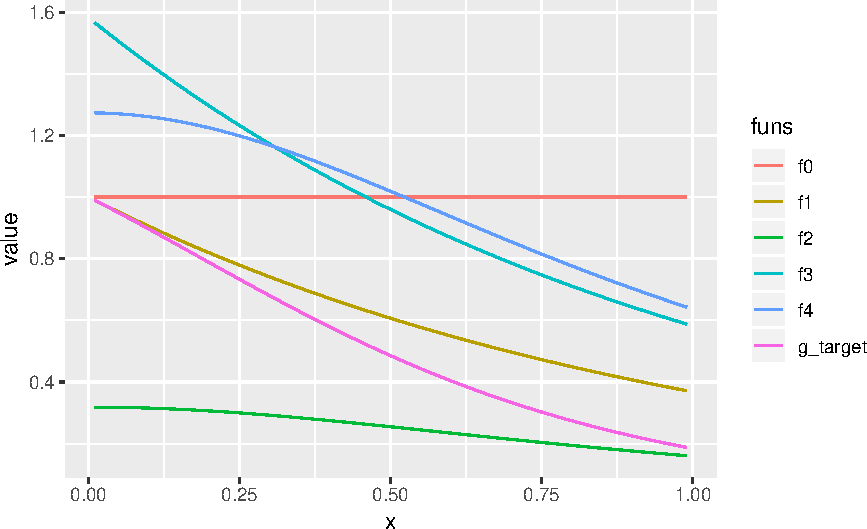
\includegraphics[width=0.7\linewidth]{statistical-computing_files/figure-latex/candimp-1} 

}

\caption{Importance funtions $\phi_0, \ldots, \phi_4$}\label{fig:candimp}
\end{figure}

Each importance function is drawn in Figure \ref{fig:candimp}. \(f_1\) shows similar patterns to \(g\).

\hypertarget{variance-in-importance-sampling}{%
\subsection{Variance in importance sampling}\label{variance-in-importance-sampling}}

From Equation \eqref{eq:impsample},

\[\theta = \int_A g(x)dx = \int_A \frac{g(x)}{\phi(x)}\phi(x) dx = E\bigg[ \frac{g(X)}{\phi(X)} \bigg] \approx \frac{1}{N} \sum \frac{g(X_i)}{\phi(X_i)}\]

where \(X_1, \ldots, X_N \stackrel{iid}{\sim}\phi\). Then

\begin{equation*}
  \begin{split}
    Var\hat\theta & = E\hat\theta^2 - (E\hat\theta)^2 \\
    & = \int_A \bigg(\frac{g(x)}{\phi(x)}\bigg)^2 \phi(x) dx - \theta^2 \\
    & = \int_A \frac{g(x)^2}{\phi(x)} dx - \theta^2
  \end{split}
\end{equation*}

Hence, the mimimum variance

\[\bigg( \int_A \lvert g(x) \rvert dx \bigg)^2 - \theta^2\]

is obtained when

\[\phi(x) = \frac{\lvert g(x) \rvert}{\int_A \lvert g(x) \rvert dx}\]

But we do not know the value of denominator. It might be hart to get the exact function giving the minimum variance, but choosing \(\phi\) close to the shape of \(\lvert g \rvert\) would produce good result. To check our criterion \eqref{eq:goodphi} more clearly, compute \(\frac{g}{\phi_i}\).

\begin{Shaded}
\begin{Highlighting}[]
\KeywordTok{tibble}\NormalTok{(}\DataTypeTok{x =} \KeywordTok{seq}\NormalTok{(.}\DecValTok{01}\NormalTok{, }\FloatTok{.99}\NormalTok{, }\DataTypeTok{by =} \FloatTok{.01}\NormalTok{)) }\OperatorTok\StringTok{ }
\StringTok{  }\KeywordTok{mutate_all}\NormalTok{(}\DataTypeTok{.funs =} \KeywordTok{list}\NormalTok{(}\OperatorTok{~}\KeywordTok{g_target}\NormalTok{(.), }\OperatorTok{~}\KeywordTok{f0}\NormalTok{(.), }\OperatorTok{~}\KeywordTok{f1}\NormalTok{(.), }\OperatorTok{~}\KeywordTok{f2}\NormalTok{(.), }\OperatorTok{~}\KeywordTok{f3}\NormalTok{(.), }\OperatorTok{~}\KeywordTok{f4}\NormalTok{(.))) }\OperatorTok\StringTok{ }
\StringTok{  }\KeywordTok{gather}\NormalTok{(}\OperatorTok{-}\NormalTok{x, }\OperatorTok{-}\NormalTok{g_target, }\DataTypeTok{key =} \StringTok{"funs"}\NormalTok{, }\DataTypeTok{value =} \StringTok{"value"}\NormalTok{) }\OperatorTok\StringTok{ }
\StringTok{  }\KeywordTok{mutate}\NormalTok{(}\DataTypeTok{value =}\NormalTok{ g_target }\OperatorTok{/}\StringTok{ }\NormalTok{value) }\OperatorTok\StringTok{ }
\StringTok{  }\KeywordTok{ggplot}\NormalTok{(}\KeywordTok{aes}\NormalTok{(}\DataTypeTok{x =}\NormalTok{ x, }\DataTypeTok{y =}\NormalTok{ value, }\DataTypeTok{colour =}\NormalTok{ funs)) }\OperatorTok{+}
\StringTok{  }\KeywordTok{geom_path}\NormalTok{()}
\end{Highlighting}
\end{Shaded}

\begin{figure}[H]

{\centering 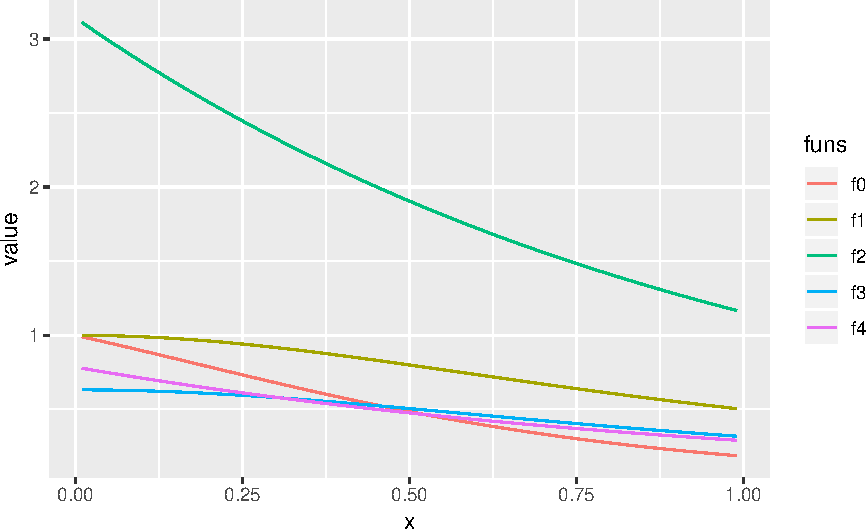
\includegraphics[width=0.7\linewidth]{statistical-computing_files/figure-latex/candimp2-1} 

}

\caption{Ratio $\frac{g}{\phi_i}$}\label{fig:candimp2}
\end{figure}

What is the closest to \(1\)? \(f_1\), of course. Would this function produce the best result, i.e.~variance?

\begin{Shaded}
\begin{Highlighting}[]
\NormalTok{theta_imp0 <-}
\StringTok{  }\KeywordTok{mc_data}\NormalTok{(runif, }\DataTypeTok{N =} \DecValTok{100}\NormalTok{)[,}
\NormalTok{                          .(}\DataTypeTok{phi0 =} \KeywordTok{mean}\NormalTok{(}\KeywordTok{g_target}\NormalTok{(u) }\OperatorTok{/}\StringTok{ }\KeywordTok{f0}\NormalTok{(u))),}
\NormalTok{                          keyby =}\StringTok{ }\NormalTok{sam]}
\end{Highlighting}
\end{Shaded}

\begin{Shaded}
\begin{Highlighting}[]
\NormalTok{theta_imp1 <-}
\StringTok{  }\KeywordTok{mc_data}\NormalTok{(rexp, }\DataTypeTok{N =} \DecValTok{100}\NormalTok{, }\DataTypeTok{rate =} \DecValTok{1}\NormalTok{)[,}
\NormalTok{                                   .(}\DataTypeTok{phi1 =} \KeywordTok{mean}\NormalTok{(}\KeywordTok{g_target}\NormalTok{(u) }\OperatorTok{/}\StringTok{ }\KeywordTok{f1}\NormalTok{(u))),}
\NormalTok{                                   keyby =}\StringTok{ }\NormalTok{sam]}
\end{Highlighting}
\end{Shaded}

\begin{Shaded}
\begin{Highlighting}[]
\NormalTok{rf2 <-}\StringTok{ }\ControlFlowTok{function}\NormalTok{(n) \{}
\NormalTok{  x <-}\StringTok{ }\KeywordTok{rcauchy}\NormalTok{(n)}
\NormalTok{  x[(x }\OperatorTok{>}\StringTok{ }\DecValTok{1}\NormalTok{) }\OperatorTok{|}\StringTok{ }\NormalTok{(x }\OperatorTok{<}\StringTok{ }\DecValTok{0}\NormalTok{)] <-}\StringTok{ }\DecValTok{2} \CommentTok{# catch overflow errors in g}
\NormalTok{  x}
\NormalTok{\}}
\NormalTok{theta_imp2 <-}
\StringTok{  }\KeywordTok{mc_data}\NormalTok{(rf2, }\DataTypeTok{N =} \DecValTok{100}\NormalTok{)[,}
\NormalTok{                        .(}\DataTypeTok{phi2 =} \KeywordTok{mean}\NormalTok{(}\KeywordTok{g_target}\NormalTok{(u) }\OperatorTok{/}\StringTok{ }\KeywordTok{f2}\NormalTok{(u))),}
\NormalTok{                        keyby =}\StringTok{ }\NormalTok{sam]}
\end{Highlighting}
\end{Shaded}

\begin{Shaded}
\begin{Highlighting}[]
\NormalTok{rf3 <-}\StringTok{ }\ControlFlowTok{function}\NormalTok{(n) \{}
\NormalTok{  u <-}\StringTok{ }\KeywordTok{runif}\NormalTok{(n)}
\NormalTok{  x <-}\StringTok{ }\OperatorTok{-}\KeywordTok{log}\NormalTok{(}\DecValTok{1} \OperatorTok{-}\StringTok{ }\NormalTok{u }\OperatorTok{*}\StringTok{ }\NormalTok{(}\DecValTok{1} \OperatorTok{-}\StringTok{ }\KeywordTok{exp}\NormalTok{(}\OperatorTok{-}\DecValTok{1}\NormalTok{))) }\CommentTok{# inverse transformation method}
\NormalTok{  x}
\NormalTok{\}}
\CommentTok{#---------------------------}
\NormalTok{theta_imp3 <-}
\StringTok{  }\KeywordTok{mc_data}\NormalTok{(rf3, }\DataTypeTok{N =} \DecValTok{100}\NormalTok{)[,}
\NormalTok{                        .(}\DataTypeTok{phi3 =} \KeywordTok{mean}\NormalTok{(}\KeywordTok{g_target}\NormalTok{(u) }\OperatorTok{/}\StringTok{ }\KeywordTok{f3}\NormalTok{(u))),}
\NormalTok{                        keyby =}\StringTok{ }\NormalTok{sam]}
\end{Highlighting}
\end{Shaded}

\begin{Shaded}
\begin{Highlighting}[]
\NormalTok{rf4 <-}\StringTok{ }\ControlFlowTok{function}\NormalTok{(n) \{}
\NormalTok{  u <-}\StringTok{ }\KeywordTok{runif}\NormalTok{(n)}
  \KeywordTok{tan}\NormalTok{(pi }\OperatorTok{*}\StringTok{ }\NormalTok{u }\OperatorTok{/}\StringTok{ }\DecValTok{4}\NormalTok{) }\CommentTok{# inverse transformation method}
\NormalTok{\}}
\CommentTok{#--------------------}
\NormalTok{theta_imp4 <-}
\StringTok{  }\KeywordTok{mc_data}\NormalTok{(rf4, }\DataTypeTok{N =} \DecValTok{100}\NormalTok{)[,}
\NormalTok{                        .(}\DataTypeTok{phi4 =} \KeywordTok{mean}\NormalTok{(}\KeywordTok{g_target}\NormalTok{(u) }\OperatorTok{/}\StringTok{ }\KeywordTok{f4}\NormalTok{(u))),}
\NormalTok{                        keyby =}\StringTok{ }\NormalTok{sam]}
\end{Highlighting}
\end{Shaded}

\begin{Shaded}
\begin{Highlighting}[]
\NormalTok{theta_imp <-}\StringTok{ }\NormalTok{theta_imp0[theta_imp1][theta_imp2][theta_imp3][theta_imp4]}
\end{Highlighting}
\end{Shaded}

\begin{Shaded}
\begin{Highlighting}[]
\NormalTok{theta_imp }\OperatorTok\StringTok{ }
\StringTok{  }\KeywordTok{melt}\NormalTok{(}\DataTypeTok{id.vars =} \StringTok{"sam"}\NormalTok{, }\DataTypeTok{variable.name =} \StringTok{"imp_fun"}\NormalTok{, }\DataTypeTok{value.name =} \StringTok{"integral"}\NormalTok{) }\OperatorTok\StringTok{ }
\StringTok{  }\KeywordTok{ggplot}\NormalTok{(}\KeywordTok{aes}\NormalTok{(}\DataTypeTok{x =}\NormalTok{ integral, }\DataTypeTok{fill =}\NormalTok{ imp_fun)) }\OperatorTok{+}
\StringTok{  }\KeywordTok{geom_histogram}\NormalTok{(}\DataTypeTok{bins =} \DecValTok{30}\NormalTok{, }\DataTypeTok{position =} \StringTok{"identity"}\NormalTok{, }\DataTypeTok{alpha =} \FloatTok{.5}\NormalTok{) }\OperatorTok{+}
\StringTok{  }\KeywordTok{xlab}\NormalTok{(}\KeywordTok{expression}\NormalTok{(theta))}
\end{Highlighting}
\end{Shaded}

\begin{figure}[H]

{\centering 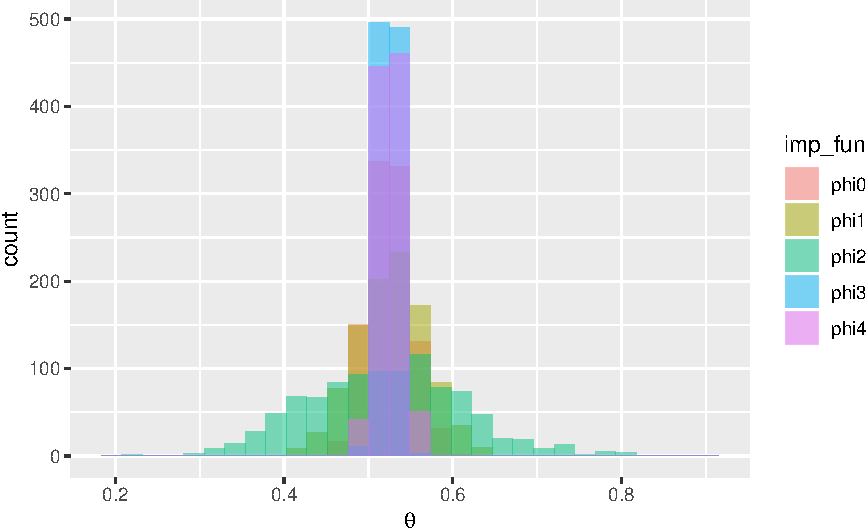
\includegraphics[width=0.7\linewidth]{statistical-computing_files/figure-latex/impcomp-1} 

}

\caption{Empirical distribution of each importance sampling}\label{fig:impcomp}
\end{figure}

\begin{Shaded}
\begin{Highlighting}[]
\NormalTok{theta_imp[,}
          \KeywordTok{lapply}\NormalTok{(.SD, sd),}
\NormalTok{          , .SDcols =}\StringTok{ }\OperatorTok{-}\StringTok{"sam"}\NormalTok{]}
\CommentTok{#>      phi0  phi1   phi2    phi3   phi4}
\CommentTok{#> 1: 0.0246 0.042 0.0941 0.00977 0.0144}
\end{Highlighting}
\end{Shaded}

\(f_3\) and possibly \(f_4\) yields the lowest variance. What happened to \(f_1\)? Its support is \((0, \infty)\), so many values would be generated outside of \((0,1)\). This results in many zeros in the sum of \(\frac{g}{f}\).

\hypertarget{monte-carlo-methods-in-inference}{%
\chapter{Monte Carlo Methods in Inference}\label{monte-carlo-methods-in-inference}}

\hypertarget{parametric-bootstrap}{%
\section{Parametric Bootstrap}\label{parametric-bootstrap}}

In this setting, we know distribution of \(X\). We can freely generate from this distribution.

\begin{figure}[H]

{\centering 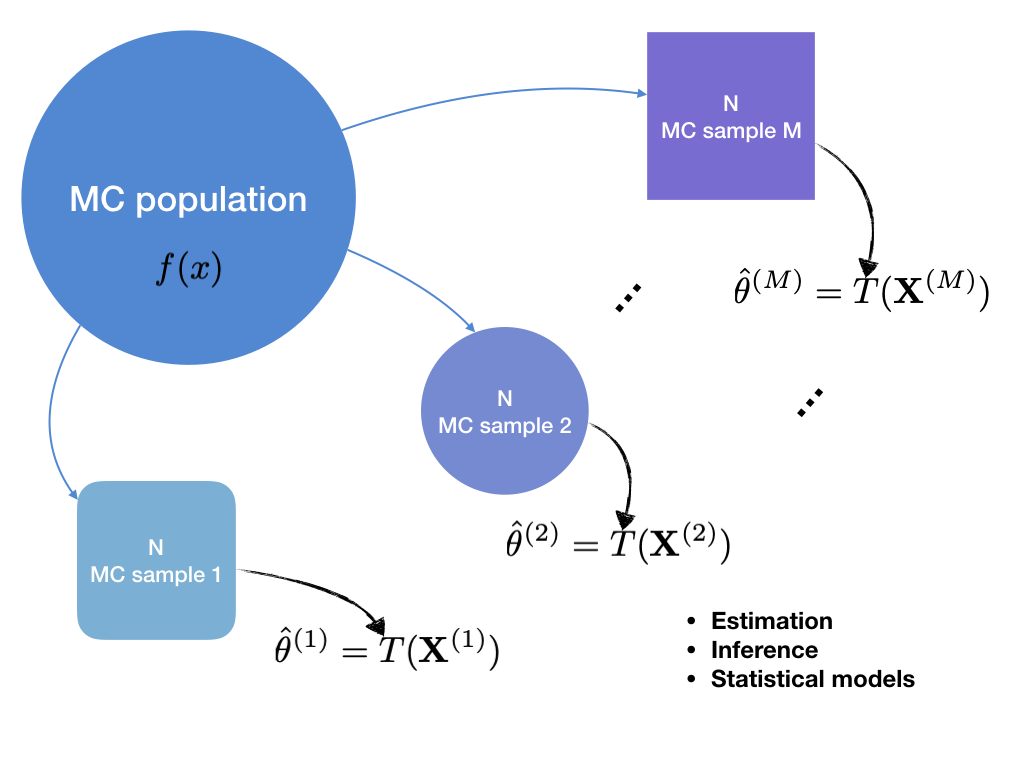
\includegraphics[width=0.7\linewidth]{images/mcboot} 

}

\caption{Parametric bootstrap}\label{fig:paramboot}
\end{figure}

See Figure \ref{fig:paramboot}. From the ``true'' distribution, we can generate multiple samples. From each sample estimator can be computed. Then we can check these multiple estimates. Multiple estimates are close to motivation of estimator, so it helps exploring statistical inference with simple steps.

\begin{Shaded}
\begin{Highlighting}[]
\NormalTok{mc_data <-}\StringTok{ }\ControlFlowTok{function}\NormalTok{(rand, }\DataTypeTok{N =} \DecValTok{10000}\NormalTok{, }\DataTypeTok{M =} \DecValTok{1000}\NormalTok{, }\DataTypeTok{char =} \StringTok{"s"}\NormalTok{, ...) \{}
  \KeywordTok{data.table}\NormalTok{(}
    \DataTypeTok{x =} \KeywordTok{rand}\NormalTok{(}\DataTypeTok{n =}\NormalTok{ N }\OperatorTok{*}\StringTok{ }\NormalTok{M, ...),}
    \DataTypeTok{sam =} \KeywordTok{gl}\NormalTok{(M, N, }\DataTypeTok{labels =} \KeywordTok{paste0}\NormalTok{(}\StringTok{"s"}\NormalTok{, }\DecValTok{1}\OperatorTok{:}\NormalTok{M))}
\NormalTok{  )}
\NormalTok{\}}
\end{Highlighting}
\end{Shaded}

\hypertarget{monte-carlo-methods-for-estimation}{%
\section{Monte Carlo Methods for Estimation}\label{monte-carlo-methods-for-estimation}}

\BeginKnitrBlock{example}[Any quantity of interest]
\protect\hypertarget{exm:quanint}{}{\label{exm:quanint} \iffalse (Any quantity of interest) \fi{} }Suppose that \(X_1, X_2 \stackrel{iid}{\sim}N(0, 1)\). We want to estimate

\[\theta = E\lvert X_1 - X_2 \rvert\]
\EndKnitrBlock{example}

\hypertarget{empirical-distribution}{%
\subsection{Empirical distribution}\label{empirical-distribution}}

\begin{algorithm}[H] \label{alg:algx1x2}
  \SetAlgoLined
  \SetKwInOut{Input}{input}
  \SetKwInOut{Output}{output}
  \Input{distribution $f$}
  \For{$m \leftarrow 1$ \KwTo $M$}{
    Generate $(X_1^{(m)}, X_2^{(m)}) \stackrel{iid}{\sim}N(0, 1)$\;
    Compute $\hat\theta^{(m)} = \lvert X_1^{(m)} - X_2^{(m)} \rvert$\;
  }
  Draw a histogram\;
  \Output{$\bar{\hat\theta} = \frac{1}{M} \sum\limits_{m = 1}^M\hat\theta_m^{(m)}, \{ \hat\theta^{(1)}, \ldots, \hat\theta^{(M)} \}$}
  \caption{Empirical distribution of $\hat\theta$}
\end{algorithm}

\begin{Shaded}
\begin{Highlighting}[]
\NormalTok{basicmc <-}
\StringTok{  }\KeywordTok{mc_data}\NormalTok{(rnorm, }\DataTypeTok{N =} \DecValTok{2}\NormalTok{)[,}
\NormalTok{                        xname }\OperatorTok{:}\ErrorTok{=}\StringTok{ }\KeywordTok{gl}\NormalTok{(}\DecValTok{2}\NormalTok{, }\DecValTok{1}\NormalTok{, }\DataTypeTok{length =} \DecValTok{2000}\NormalTok{, }\DataTypeTok{labels =} \KeywordTok{c}\NormalTok{(}\StringTok{"x1"}\NormalTok{, }\StringTok{"x2"}\NormalTok{))] }\OperatorTok\StringTok{ }
\StringTok{  }\KeywordTok{dcast}\NormalTok{(sam }\OperatorTok{~}\StringTok{ }\NormalTok{xname, }\DataTypeTok{value.var =} \StringTok{"x"}\NormalTok{) }\OperatorTok\StringTok{ }
\StringTok{  }\NormalTok{.[,}
\NormalTok{    .(}\DataTypeTok{that =} \KeywordTok{mean}\NormalTok{(}\KeywordTok{abs}\NormalTok{(x1 }\OperatorTok{-}\StringTok{ }\NormalTok{x2))),}
\NormalTok{    by =}\StringTok{ }\NormalTok{sam]}
\end{Highlighting}
\end{Shaded}

\begin{Shaded}
\begin{Highlighting}[]
\NormalTok{basicmc[,}
\NormalTok{        .(}\DataTypeTok{est =} \KeywordTok{mean}\NormalTok{(that))]}
\CommentTok{#>    est}
\CommentTok{#> 1: 1.1}
\end{Highlighting}
\end{Shaded}

\begin{Shaded}
\begin{Highlighting}[]
\NormalTok{basicmc }\OperatorTok\StringTok{ }
\StringTok{  }\KeywordTok{ggplot}\NormalTok{(}\KeywordTok{aes}\NormalTok{(}\DataTypeTok{x =}\NormalTok{ that)) }\OperatorTok{+}
\StringTok{  }\KeywordTok{geom_histogram}\NormalTok{(}\DataTypeTok{bins =} \DecValTok{30}\NormalTok{, }\DataTypeTok{col =} \KeywordTok{gg_hcl}\NormalTok{(}\DecValTok{1}\NormalTok{), }\DataTypeTok{alpha =} \FloatTok{.7}\NormalTok{) }\OperatorTok{+}
\StringTok{  }\KeywordTok{xlab}\NormalTok{(}\KeywordTok{expression}\NormalTok{(theta))}
\end{Highlighting}
\end{Shaded}

\begin{figure}[H]

{\centering 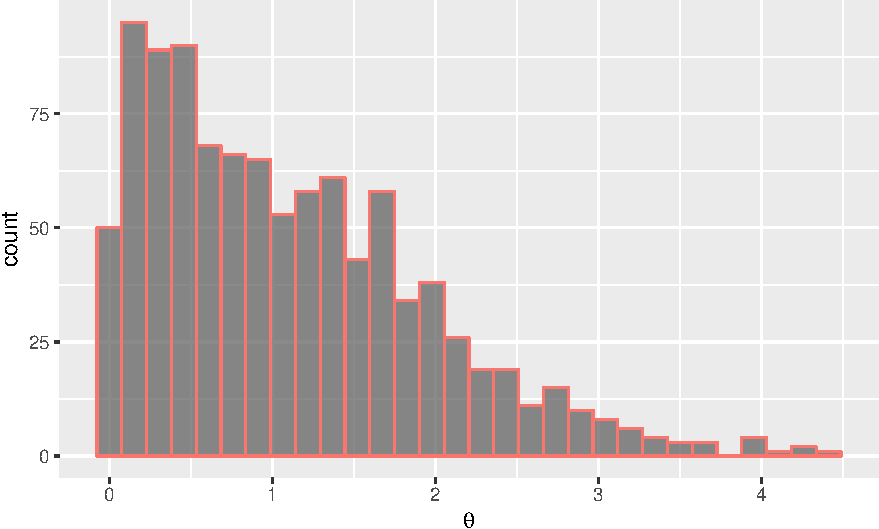
\includegraphics[width=0.7\linewidth]{statistical-computing_files/figure-latex/absx12-1} 

}

\caption{Empirical distribution of $\hat\theta$ for $\lvert X_1 - X_2 \rvert$}\label{fig:absx12}
\end{figure}

\hypertarget{standard-error}{%
\subsection{Standard error}\label{standard-error}}

In Algorithm \(\ref{alg:algx1x2}\), we can get standard error by just calculating standard deviation of

\[\{ \hat\theta^{(1)}, \ldots, \hat\theta^{(M)} \}\]

\begin{algorithm}[H] \label{alg:algmcse}
  \SetAlgoLined
  \SetKwInOut{Input}{input}
  \SetKwInOut{Output}{output}
  \Input{distribution $f$}
  \For{$m \leftarrow 1$ \KwTo $M$}{
    Generate $(X_1^{(m)}, X_2^{(m)}) \stackrel{iid}{\sim}N(0, 1)$\;
    Compute $\hat\theta^{(m)} = \lvert X_1^{(m)} - X_2^{(m)} \rvert$\;
  }
  $\bar{\hat\theta} = \frac{1}{M} \sum\limits_{m = 1}^M\hat\theta_m^{(m)}$\;
  $\widehat{SE}(\hat\theta) = \sqrt{\frac{1}{M - 1}\sum\limits_{m = 1}^M(\hat\theta^{(m)} - \bar{\hat\theta})}$\;
  \Output{$\widehat{SE}(\hat\theta)$}
  \caption{Standard error of $\hat\theta$}
\end{algorithm}

\begin{Shaded}
\begin{Highlighting}[]
\NormalTok{basicmc[,}
\NormalTok{        .(}\DataTypeTok{se =} \KeywordTok{sd}\NormalTok{(that))]}
\CommentTok{#>       se}
\CommentTok{#> 1: 0.844}
\end{Highlighting}
\end{Shaded}

\hypertarget{mean-squared-error}{%
\subsection{Mean squared error}\label{mean-squared-error}}

\(MSE\) is used when comparing several estimators.

\BeginKnitrBlock{definition}[Mean squared error]
\protect\hypertarget{def:mse}{}{\label{def:mse} \iffalse (Mean squared error) \fi{} }\[MSE(\hat\theta) := E(\hat\theta - \theta)^2\]
\EndKnitrBlock{definition}

To know \(MSE\), however, we should compute expectation. Some of them might be complicated even though we know true distribution. As the last chapter, we can apply Monte carlo method.

\BeginKnitrBlock{example}[MSE of a trimmed mean]
\protect\hypertarget{exm:trim}{}{\label{exm:trim} \iffalse (MSE of a trimmed mean) \fi{} }Suppose that \(X_1, \ldots, X_n \stackrel{iid}{\sim}N(2, 1)\). Consider three estimators for \(\mu = 2\).

\begin{enumerate}
  \item mean $\overline{X}$
  \item median $\tilde{X}$
  \item $k$th trimmed mean $\overline{X}_{[-k]}$
\end{enumerate}
\EndKnitrBlock{example}

\begin{algorithm}[H] \label{alg:algmse}
  \SetAlgoLined
  \SetKwInOut{Input}{input}
  \SetKwInOut{Output}{output}
  \Input{distribution $f$}
  \For{$m \leftarrow 1$ \KwTo $M$}{
    Generate $(X_1^{(m)}, \ldots, X_N^{(m)}) \stackrel{iid}{\sim}N(2, 1)$\;
    Sort $(X_1^{(m)}, \ldots, X_N^{(m)})$ in increasing order, i.e. $(X_{(1)}^{(m)}, \ldots, X_{(N)}^{(m)})$\;
    Mean $\overline{X}^{(m)} = \frac{1}{N}\sum\limits_{i = 1}^N X_i^{(m)}$\;
    Median $\tilde{X}^{(m)} = \begin{cases} X_{\frac{N}{2} + 1}^{(m)} & N \:\text{odd} \\ \frac{X_{\frac{N}{2}}^{(m)} + X_{\frac{N}{2} + 1}^{(m)}}{2} & N \:\text{even} \end{cases}$\;
    $k$th trimmed mean $\overline{X}_{[-k]}^{(m)} = \frac{1}{N - 2k}\sum\limits_{i = k + 1}^{n - k}X_{(i)}^{(m)}$
  }
  $\widehat{MSE}(\overline{X}) = \frac{1}{M} \sum\limits_{m = 1}^M (\overline{X}^{(m)} - 2)^2$\;
  $\widehat{MSE}(\tilde{X}) = \frac{1}{M} \sum\limits_{m = 1}^M (\tilde{X}^{(m)} - 2)^2$\;
  $\widehat{MSE}(\overline{X}_{[-k]}) = \frac{1}{M} \sum\limits_{m = 1}^M (\overline{X}_{[-k]}^{(m)} - 2)^2$\;
  \Output{$\widehat{MSE}(\overline{X}), \widehat{MSE}(\tilde{X}), \:\text{and}\: \widehat{MSE}(\overline{X}_{[-k]})$}
  \caption{MSE of mean, median, and $k$th trimmed mean}
\end{algorithm}

\begin{Shaded}
\begin{Highlighting}[]
\NormalTok{trim <-}\StringTok{ }\ControlFlowTok{function}\NormalTok{(x, }\DataTypeTok{k =} \DecValTok{1}\NormalTok{) \{}
\NormalTok{  n <-}\StringTok{ }\KeywordTok{length}\NormalTok{(x)}
\NormalTok{  x <-}\StringTok{ }\KeywordTok{sort}\NormalTok{(x)}
  \KeywordTok{sum}\NormalTok{(x[(k }\OperatorTok{+}\StringTok{ }\DecValTok{1}\NormalTok{)}\OperatorTok{:}\NormalTok{(n }\OperatorTok{-}\StringTok{ }\NormalTok{k)]) }\OperatorTok{/}\StringTok{ }\NormalTok{(n }\OperatorTok{-}\StringTok{ }\DecValTok{2} \OperatorTok{*}\StringTok{ }\NormalTok{k)}
\NormalTok{\}}
\CommentTok{#--------------------------------------}
\NormalTok{mu_list <-}\StringTok{ }\ControlFlowTok{function}\NormalTok{(x, k) \{}
  \KeywordTok{list}\NormalTok{(}\DataTypeTok{mean =} \KeywordTok{mean}\NormalTok{(x), }\DataTypeTok{median =} \KeywordTok{median}\NormalTok{(x), }\DataTypeTok{trim =} \KeywordTok{trim}\NormalTok{(x, k))}
\NormalTok{\}}
\end{Highlighting}
\end{Shaded}

Try \(k = 1\).

\begin{Shaded}
\begin{Highlighting}[]
\NormalTok{(trim_mc <-}
\StringTok{  }\KeywordTok{mc_data}\NormalTok{(rnorm, }\DataTypeTok{mean =} \DecValTok{2}\NormalTok{, }\DataTypeTok{sd =} \DecValTok{1}\NormalTok{)[,}
                                   \KeywordTok{unlist}\NormalTok{(}\KeywordTok{lapply}\NormalTok{(.SD, mu_list, }\DataTypeTok{k =} \DecValTok{1}\NormalTok{)) }\OperatorTok\StringTok{ }\NormalTok{as.list,}
                                   \DataTypeTok{by =}\NormalTok{ sam])}
\CommentTok{#>         sam x.mean x.median x.trim}
\CommentTok{#>    1:    s1   2.02     2.02   2.02}
\CommentTok{#>    2:    s2   2.00     2.00   2.00}
\CommentTok{#>    3:    s3   2.00     2.01   2.00}
\CommentTok{#>    4:    s4   1.99     1.98   1.99}
\CommentTok{#>    5:    s5   2.00     1.99   2.00}
\CommentTok{#>   ---                             }
\CommentTok{#>  996:  s996   2.02     2.02   2.02}
\CommentTok{#>  997:  s997   2.00     1.99   2.00}
\CommentTok{#>  998:  s998   1.99     1.99   1.99}
\CommentTok{#>  999:  s999   1.99     1.99   1.99}
\CommentTok{#> 1000: s1000   2.00     2.01   2.00}
\end{Highlighting}
\end{Shaded}

\begin{Shaded}
\begin{Highlighting}[]
\NormalTok{trim_mc }\OperatorTok\StringTok{ }
\StringTok{  }\KeywordTok{melt}\NormalTok{(}\DataTypeTok{id.vars =} \StringTok{"sam"}\NormalTok{, }\DataTypeTok{variable.name =} \StringTok{"hat"}\NormalTok{) }\OperatorTok\StringTok{ }
\StringTok{  }\KeywordTok{ggplot}\NormalTok{(}\KeywordTok{aes}\NormalTok{(}\DataTypeTok{x =}\NormalTok{ value, }\DataTypeTok{fill =}\NormalTok{ hat)) }\OperatorTok{+}
\StringTok{  }\KeywordTok{geom_histogram}\NormalTok{(}\DataTypeTok{bins =} \DecValTok{30}\NormalTok{, }\DataTypeTok{alpha =} \FloatTok{.3}\NormalTok{, }\DataTypeTok{position =} \StringTok{"identity"}\NormalTok{) }\OperatorTok{+}
\StringTok{  }\KeywordTok{xlab}\NormalTok{(}\KeywordTok{expression}\NormalTok{(mu)) }\OperatorTok{+}
\StringTok{  }\KeywordTok{geom_vline}\NormalTok{(}\DataTypeTok{xintercept =} \DecValTok{2}\NormalTok{, }\DataTypeTok{col =} \KeywordTok{I}\NormalTok{(}\StringTok{"red"}\NormalTok{)) }\OperatorTok{+}
\StringTok{  }\KeywordTok{scale_fill_discrete}\NormalTok{(}
    \DataTypeTok{name =} \StringTok{"Estimates"}\NormalTok{,}
    \DataTypeTok{labels =} \KeywordTok{c}\NormalTok{(}\StringTok{"Mean"}\NormalTok{, }\StringTok{"Median"}\NormalTok{, }\StringTok{"Trimmed"}\NormalTok{)}
\NormalTok{  )}
\end{Highlighting}
\end{Shaded}

\begin{figure}[H]

{\centering 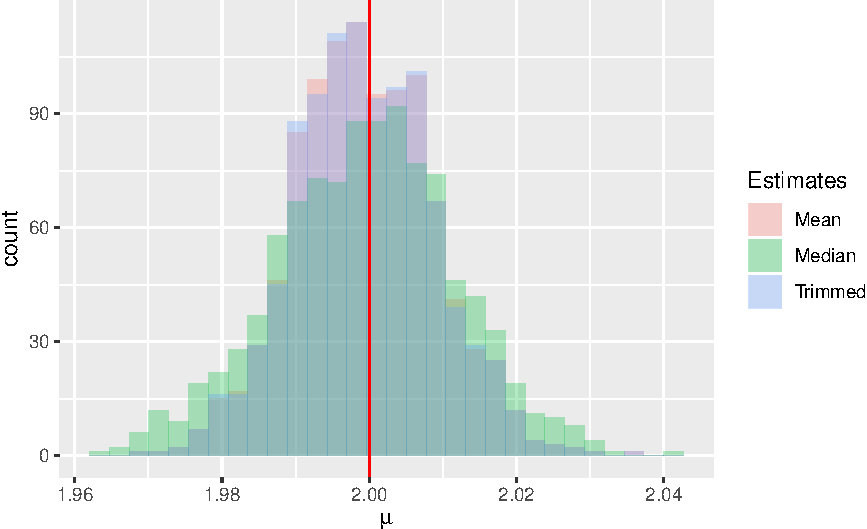
\includegraphics[width=0.7\linewidth]{statistical-computing_files/figure-latex/meanemp-1} 

}

\caption{Empirical distribution of each estimator for $\mu = 2$}\label{fig:meanemp}
\end{figure}

Here, median shows the largest standard error.

\begin{Shaded}
\begin{Highlighting}[]
\NormalTok{trim_mc[,}
        \KeywordTok{lapply}\NormalTok{(.SD, sd),}
\NormalTok{        .SDcols =}\StringTok{ }\OperatorTok{-}\StringTok{"sam"}\NormalTok{]}
\CommentTok{#>     x.mean x.median  x.trim}
\CommentTok{#> 1: 0.00942   0.0123 0.00942}
\end{Highlighting}
\end{Shaded}

Now try various \(k\) for trimmed mean.

\begin{Shaded}
\begin{Highlighting}[]
\NormalTok{mse_list <-}\StringTok{ }\ControlFlowTok{function}\NormalTok{(x, k) \{}
  \KeywordTok{list}\NormalTok{(}\DataTypeTok{mse =} \KeywordTok{mean}\NormalTok{((x }\OperatorTok{-}\StringTok{ }\DecValTok{2}\NormalTok{)}\OperatorTok{^}\DecValTok{2}\NormalTok{), }\DataTypeTok{se =} \KeywordTok{sd}\NormalTok{(x))}
\NormalTok{\}}
\CommentTok{#-----------------------------------------}
\NormalTok{trim_mse <-}
\StringTok{  }\KeywordTok{mc_data}\NormalTok{(rnorm, }\DataTypeTok{mean =} \DecValTok{2}\NormalTok{, }\DataTypeTok{sd =} \DecValTok{1}\NormalTok{)[,}
                                   \KeywordTok{lapply}\NormalTok{(.SD, }\ControlFlowTok{function}\NormalTok{(x) \{}
                                     \KeywordTok{sapply}\NormalTok{(}\DecValTok{0}\OperatorTok{:}\DecValTok{9}\NormalTok{, }\ControlFlowTok{function}\NormalTok{(k) \{}
                                       \KeywordTok{trim}\NormalTok{(}\DataTypeTok{x =}\NormalTok{ x, }\DataTypeTok{k =}\NormalTok{ k)}
\NormalTok{                                     \})}
\NormalTok{                                   \}) }\OperatorTok\StringTok{ }
\StringTok{                                     }\KeywordTok{unlist}\NormalTok{() }\OperatorTok\StringTok{ }
\StringTok{                                     }\KeywordTok{as.list}\NormalTok{(),}
\NormalTok{                                   by =}\StringTok{ }\NormalTok{sam][,}
                                             \KeywordTok{lapply}\NormalTok{(.SD, mse_list) }\OperatorTok\StringTok{ }
\StringTok{                                               }\KeywordTok{unlist}\NormalTok{() }\OperatorTok\StringTok{ }
\StringTok{                                               }\KeywordTok{as.list}\NormalTok{(),}
\NormalTok{                                             .SDcols =}\StringTok{ }\OperatorTok{-}\StringTok{"sam"}\NormalTok{]}
\end{Highlighting}
\end{Shaded}

\begin{Shaded}
\begin{Highlighting}[]
\NormalTok{trim_mse }\OperatorTok\StringTok{ }
\StringTok{  }\KeywordTok{transpose}\NormalTok{() }\OperatorTok\StringTok{ }
\StringTok{  }\NormalTok{.[,}
    \StringTok{`}\DataTypeTok{:=}\StringTok{`}\NormalTok{(}
      \DataTypeTok{k =} \KeywordTok{rep}\NormalTok{(}\DecValTok{0}\OperatorTok{:}\DecValTok{9}\NormalTok{, }\DataTypeTok{each =} \DecValTok{2}\NormalTok{),}
      \DataTypeTok{hat =} \KeywordTok{gl}\NormalTok{(}\DecValTok{2}\NormalTok{, }\DataTypeTok{k =} \DecValTok{1}\NormalTok{, }\DataTypeTok{length =} \DecValTok{2} \OperatorTok{*}\StringTok{ }\DecValTok{10}\NormalTok{, }\DataTypeTok{labels =} \KeywordTok{c}\NormalTok{(}\StringTok{"mse"}\NormalTok{, }\StringTok{"se"}\NormalTok{))}
\NormalTok{    )] }\OperatorTok\StringTok{ }
\StringTok{  }\KeywordTok{dcast}\NormalTok{(k }\OperatorTok{~}\StringTok{ }\NormalTok{hat, }\DataTypeTok{value.var =} \StringTok{"V1"}\NormalTok{)}
\CommentTok{#>     k      mse      se}
\CommentTok{#>  1: 0 9.83e-05 0.00992}
\CommentTok{#>  2: 1 9.83e-05 0.00992}
\CommentTok{#>  3: 2 9.83e-05 0.00992}
\CommentTok{#>  4: 3 9.83e-05 0.00992}
\CommentTok{#>  5: 4 9.82e-05 0.00992}
\CommentTok{#>  6: 5 9.83e-05 0.00992}
\CommentTok{#>  7: 6 9.83e-05 0.00992}
\CommentTok{#>  8: 7 9.83e-05 0.00992}
\CommentTok{#>  9: 8 9.83e-05 0.00992}
\CommentTok{#> 10: 9 9.83e-05 0.00992}
\end{Highlighting}
\end{Shaded}

\hypertarget{confidence-interval}{%
\section{Confidence interval}\label{confidence-interval}}

Remember the meaning of 95\% confidence interval. \emph{If we have 100 samples and construct confidence interval in each sample, 95 intervals would include true parameter}. In this Monte Carlo setting, we know true population distribution, so we can generate multiple samples. Thus, we can reproduce this confidence interval situation.

\hypertarget{empirical-confidence-interval}. Best critical region leads to the shortest length of CI given \(\alpha\), so we are finding this one.

\begin{algorithm}[H] \label{alg:algempci}
  \SetAlgoLined
  \SetKwInOut{Input}{input}
  \SetKwInOut{Output}{output}
  \Input{distribution $f$}
  \For{$m \leftarrow 1$ \KwTo $M$}{
    Generate $X_1^{(m)}, \ldots, X_n^{(m)} \stackrel{iid}{\sim}f$\;
    Compute $\hat\theta^{(m)} = \hat\theta(\mathbf{\mathbf{X}^{(m)}})$\;
  }
  \eIf{Distribution of $\{ \hat\theta^{(m)} \}_1^M$ symmetric}{
    Sort $\{ \hat\theta^{(1)}, \ldots, \hat\theta^{(M)} \}$ in decreasing order, i.e. $\{ \hat\theta_{(1)}^{(1)}, \ldots, \hat\theta_{(M)}^{(M)} \}$\;
    Compute $LB= \frac{\alpha}{2} \:\text{sample quantile}$ and $UB= 1 - \frac{\alpha}{2} \:\text{sample quantile}$\;
  }{
    \ForEach{$lb < 0.05$ with $ub - lb = 1 - \alpha$}{
      Candidate interval $(lb, ub)$\;
      calculate length $l_i = ub - lb$\;
    }
    $(LB, UB)$: pick up the interval with the smallest length $l_i$\;
  }
  \Output{$(LB, UB)$}
  \caption{Empirical confidence interval by Monte Carlo method}
\end{algorithm}

\hypertarget{empirical-confidence-level}{%
\subsection{Empirical confidence level}\label{empirical-confidence-level}}

On the contrary, we can estiamte confidence level given confidence interval.

\BeginKnitrBlock{example}[Confidence interval for variance]
\protect\hypertarget{exm:civar}{}{\label{exm:civar} \iffalse (Confidence interval for variance) \fi{} }If \(X_1, \ldots, X_n \stackrel{iid}{\sim}N(\mu, \sigma^2)\), then

\[T = \frac{(n - 1)S^2}{\sigma^2} \sim \chi^2(n - 1)\]

Thus, \(100(1 - \alpha)\%\) confidence interval is given by

\[(0, \frac{(n -1)S^2}{\chi^2_{\alpha}(n - 1)})\]
\EndKnitrBlock{example}

For each MC sample, compute confidence interval. Just check if \emph{known true parameter} is in the interval. Its proportion becomes the confidence level. It is simpler that estimate confidence interval itself.

\begin{algorithm}[H] \label{alg:algcilev}
  \SetAlgoLined
  \SetKwInOut{Input}{input}
  \SetKwInOut{Output}{output}
  \Input{distribution $f$ with parameter $\theta$}
  \For{$m \leftarrow 1$ \KwTo $M$}{
    Generate $X_1^{(m)}, \ldots, X_n^{(m)} \stackrel{iid}{\sim}f$\;
    Compute the confidence interval $C_m$\;
    Compute $Y_j = I(\theta \in C_m)$, i.e. whether $\theta$ is in the CI\;
  }
  Empirical confidence level $\overline{Y} = \sum\limits_{m = 1}^M Y_m$\; \label{alg:cilevlast}
  \Output{$\overline{Y}$}
  \caption{Empirical confidence level by Monte Carlo method}
\end{algorithm}

Let \(\mu = 0\), \(\sigma = 2\), \(N = 20\), and let \(M = 1000\).

\begin{Shaded}
\begin{Highlighting}[]
\NormalTok{ci_var <-}\StringTok{ }\ControlFlowTok{function}\NormalTok{(x, variance, alpha) \{}
\NormalTok{  n <-}\StringTok{ }\KeywordTok{length}\NormalTok{(x)}
\NormalTok{  s2 <-}\StringTok{ }\KeywordTok{var}\NormalTok{(x)}
\NormalTok{  (n }\OperatorTok{-}\StringTok{ }\DecValTok{1}\NormalTok{) }\OperatorTok{*}\StringTok{ }\NormalTok{s2 }\OperatorTok{/}\StringTok{ }\KeywordTok{qchisq}\NormalTok{(alpha, }\DataTypeTok{df =}\NormalTok{ n }\OperatorTok{-}\StringTok{ }\DecValTok{1}\NormalTok{) }\OperatorTok{>}\StringTok{ }\NormalTok{variance}
\NormalTok{\}}
\CommentTok{#---------------------------}
\NormalTok{ci_lev <-}
\StringTok{  }\KeywordTok{mc_data}\NormalTok{(rnorm, }\DataTypeTok{N =} \DecValTok{20}\NormalTok{, }\DataTypeTok{M =} \DecValTok{1000}\NormalTok{, }\DataTypeTok{mean =} \DecValTok{0}\NormalTok{, }\DataTypeTok{sd =} \DecValTok{2}\NormalTok{)[,}
\NormalTok{                                                     .(}\DataTypeTok{hat =} \KeywordTok{mean}\NormalTok{(}\KeywordTok{ci_var}\NormalTok{(x, }\DataTypeTok{variance =} \DecValTok{4}\NormalTok{, }\DataTypeTok{alpha =} \FloatTok{.05}\NormalTok{))),}
\NormalTok{                                                     by =}\StringTok{ }\NormalTok{sam]}
\end{Highlighting}
\end{Shaded}

\begin{Shaded}
\begin{Highlighting}[]
\NormalTok{ci_lev[,}
\NormalTok{       .N,}
\NormalTok{       by =}\StringTok{ }\NormalTok{hat][,}
\NormalTok{                 proportion }\OperatorTok{:}\ErrorTok{=}\StringTok{ }\NormalTok{N }\OperatorTok{/}\StringTok{ }\KeywordTok{sum}\NormalTok{(N)] }\OperatorTok
\StringTok{  }\KeywordTok{ggplot}\NormalTok{(}\KeywordTok{aes}\NormalTok{(}\DataTypeTok{x =}\NormalTok{ hat, }\DataTypeTok{y =}\NormalTok{ proportion, }\DataTypeTok{fill =} \KeywordTok{factor}\NormalTok{(hat))) }\OperatorTok{+}
\StringTok{  }\KeywordTok{geom_bar}\NormalTok{(}\DataTypeTok{stat =} \StringTok{"identity"}\NormalTok{) }\OperatorTok{+}
\StringTok{  }\KeywordTok{scale_fill_discrete}\NormalTok{(}
    \DataTypeTok{name =} \StringTok{"CI"}\NormalTok{,}
    \DataTypeTok{labels =} \KeywordTok{c}\NormalTok{(}\StringTok{"out"}\NormalTok{, }\StringTok{"in"}\NormalTok{)}
\NormalTok{  ) }\OperatorTok{+}
\StringTok{  }\KeywordTok{xlab}\NormalTok{(}\KeywordTok{expression}\NormalTok{(y))}
\end{Highlighting}
\end{Shaded}

\begin{figure}[H]

{\centering 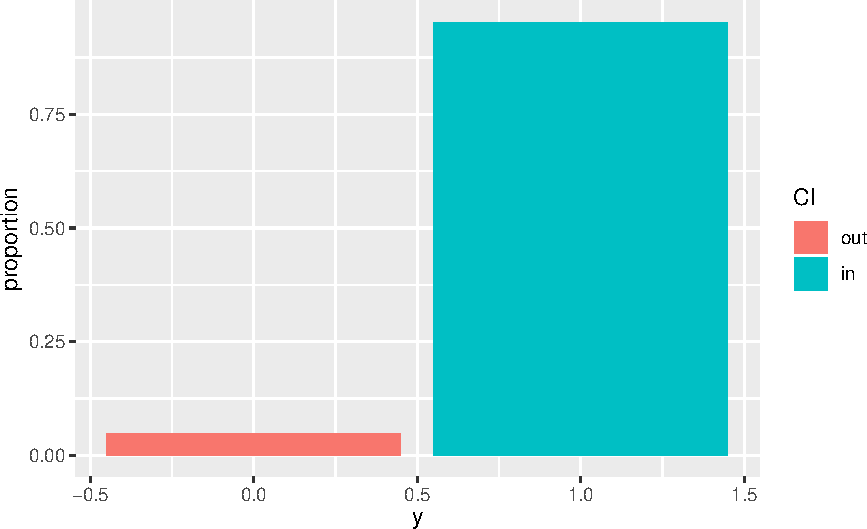
\includegraphics[width=0.7\linewidth]{statistical-computing_files/figure-latex/ciin-1} 

}

\caption{Proportion of $\sigma^2$ in confidence intervals}\label{fig:ciin}
\end{figure}

This leads to empirical confidence level, i.e.~\emph{sample proportion}. Just follow the last step \(\ref{alg:cilevlast}\) of Algorithm \(\ref{alg:algcilev}\).

\begin{Shaded}
\begin{Highlighting}[]
\NormalTok{(ci_lev <-}
\StringTok{  }\NormalTok{ci_lev[,}
\NormalTok{         .(}\DataTypeTok{level =} \KeywordTok{mean}\NormalTok{(hat))])}
\CommentTok{#>    level}
\CommentTok{#> 1: 0.952}
\end{Highlighting}
\end{Shaded}

It is very close to \(0.95\). One of advantages of simulation study is we can assume various situation. For example, \emph{violation of Gausiannity}.

\BeginKnitrBlock{example}[Violation of Normal distribution assumption]
\protect\hypertarget{exm:nonnormal}{}{\label{exm:nonnormal} \iffalse (Violation of Normal distribution assumption) \fi{} }Refer to Example \ref{exm:civar}. This has assumed that \(X_i \stackrel{iid}{\sim}N(\mu = 2, \sigma^2 = 4)\). What if not? For instance,

\[X_1, \ldots, X_n \stackrel{iid}{\sim}\chi^2(df = 2)\]
\EndKnitrBlock{example}

Just change random numbers.

\begin{Shaded}
\begin{Highlighting}[]
\NormalTok{ci_lev2 <-}
\StringTok{  }\KeywordTok{mc_data}\NormalTok{(rchisq, }\DataTypeTok{N =} \DecValTok{20}\NormalTok{, }\DataTypeTok{M =} \DecValTok{1000}\NormalTok{, }\DataTypeTok{df =} \DecValTok{2}\NormalTok{)[,}
\NormalTok{                                            .(}\DataTypeTok{hat =} \KeywordTok{mean}\NormalTok{(}\KeywordTok{ci_var}\NormalTok{(x, }\DataTypeTok{variance =} \DecValTok{4}\NormalTok{, }\DataTypeTok{alpha =} \FloatTok{.05}\NormalTok{))),}
\NormalTok{                                            by =}\StringTok{ }\NormalTok{sam][,}
\NormalTok{                                                      .(}\DataTypeTok{non_normal =} \KeywordTok{mean}\NormalTok{(hat))]}
\end{Highlighting}
\end{Shaded}

\begin{longtable}{r|r}
\caption{\label{tab:emlevpop}Empirical confidence level for each population}\\
\hline
Normal & Chisq\\
\hline
0.952 & 0.763\\
\hline
\end{longtable}

From Table \ref{tab:emlevpop}, we found that \emph{non-normality lowers confidence level} from 0.952 to 0.763.

\hypertarget{hypothesis-tests}{%
\section{Hypothesis tests}\label{hypothesis-tests}}

Using MC method, we have done point estimation and interval estimation. Now consider \emph{hypothesis testing}.

\[H_0: \theta \in \Theta_0 \qquad \text{vs} \qquad H_1: \theta \in \Theta_1\]

where \(\{ \Theta_0, \Theta_1 \}\) is a partition of the parameter space \(\Theta\). First of all, we have \emph{test statistic}

\[T(\mathbf{X}) \stackrel{H_0}{\sim}f\]

and \(f\) is called \emph{null distribution}. Given observed data, we compute this test statistic \(T_0\). Where \(T_0\) is located in the null distribution \(f\) decides whether we reject or accept \(H_0\). If \(T_0\) is very far from the middle, we can say that the realized data set is very rare event under \(H_0\). In this case, we reject \(H_0\). Otherwise, accept it. This is why we compute the tail probability, p-value.

\hypertarget{empirical-p-value}{%
\subsection{Empirical p-value}\label{empirical-p-value}}

\BeginKnitrBlock{example}
\protect\hypertarget{exm:exptest}{}{\label{exm:exptest} }Suppose that \(X_1, \ldots, X_{10} \stackrel{iid}{\sim}Exp(\lambda = 1)\), which are observed as follows

\[`r xexp`\]

Let \(\theta = E(X) = \frac{1}{\lambda}\).

\[H_0: \theta = 0.5 \qquad \text{vs} \qquad H_1: \theta > 0.5\]

Test using \(T = \frac{\overline{X} - \theta_0}{S / \sqrt{n}}\) statistic.
\EndKnitrBlock{example}

Before looking at p-value, briefly look at \emph{empirical null distribution} of test statistic.

\begin{Shaded}
\begin{Highlighting}[]
\KeywordTok{mc_data}\NormalTok{(rexp, }\DataTypeTok{rate =} \DecValTok{2}\NormalTok{)[,}
\NormalTok{                        .(}\DataTypeTok{tstat =} \KeywordTok{t.test}\NormalTok{(x, }\DataTypeTok{mu =} \FloatTok{.5}\NormalTok{)}\OperatorTok{$}\NormalTok{statistic),}
\NormalTok{                        by =}\StringTok{ }\NormalTok{sam] }\OperatorTok\StringTok{ }
\StringTok{  }\KeywordTok{ggplot}\NormalTok{(}\KeywordTok{aes}\NormalTok{(}\DataTypeTok{x =}\NormalTok{ tstat)) }\OperatorTok{+}
\StringTok{  }\KeywordTok{geom_histogram}\NormalTok{(}\DataTypeTok{bins =} \DecValTok{30}\NormalTok{, }\DataTypeTok{col =} \KeywordTok{gg_hcl}\NormalTok{(}\DecValTok{1}\NormalTok{), }\DataTypeTok{alpha =} \FloatTok{.7}\NormalTok{) }\OperatorTok{+}
\StringTok{  }\KeywordTok{geom_vline}\NormalTok{(}\DataTypeTok{xintercept =} \KeywordTok{t.test}\NormalTok{(xexp, }\DataTypeTok{mu =} \FloatTok{.5}\NormalTok{)}\OperatorTok{$}\NormalTok{statistic, }\DataTypeTok{col =} \KeywordTok{I}\NormalTok{(}\StringTok{"red"}\NormalTok{)) }\OperatorTok{+}\StringTok{ }\CommentTok{# xexp: observed data}
\StringTok{  }\KeywordTok{geom_vline}\NormalTok{(}\DataTypeTok{xintercept =} \OperatorTok{-}\KeywordTok{t.test}\NormalTok{(xexp, }\DataTypeTok{mu =} \FloatTok{.5}\NormalTok{)}\OperatorTok{$}\NormalTok{statistic, }\DataTypeTok{col =} \KeywordTok{I}\NormalTok{(}\StringTok{"red"}\NormalTok{)) }\OperatorTok{+}
\StringTok{  }\KeywordTok{xlab}\NormalTok{(}\StringTok{"T"}\NormalTok{)}
\end{Highlighting}
\end{Shaded}

\begin{figure}[H]

{\centering 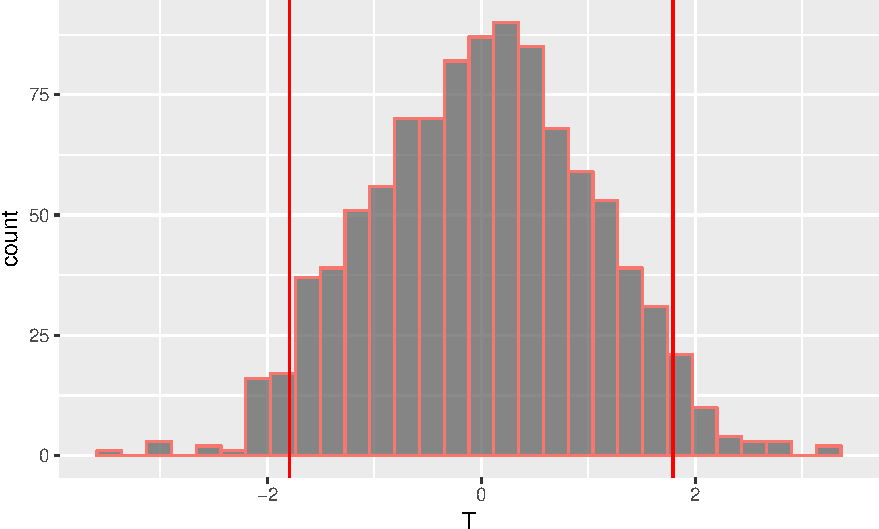
\includegraphics[width=0.7\linewidth]{statistical-computing_files/figure-latex/expemp-1} 

}

\caption{Emprirical Null Distribution}\label{fig:expemp}
\end{figure}

By proceeding the similar way, we can get empirical distribution of test statistics. Some are out of observed \(T_0\), some are not. Motivation is that we just count these. Proportion of these would estimate p-value. Recap what p-value is.

\BeginKnitrBlock{definition}[p-value]
\protect\hypertarget{def:pval}{}{\label{def:pval} \iffalse (p-value) \fi{} }Let \(T\) be test statistic and let \(T_0\) be observed test statistic given data. Then p-value is

\[
p-value := \begin{cases}
  P(\lvert T \rvert \ge T_0 \mid H_0) & \text{both sided} \\
  P(T \ge T_0 \mid H_0) & \text{one sided} \\
  P(T \le T_0 \mid H_0) & \text{one sided}
\end{cases}
\]
\EndKnitrBlock{definition}

Denote that p-value is probability. So in MC setting, we can estimate this by computing \emph{sample mean of identity function}.

\BeginKnitrBlock{lemma}[Empirical p-value]
\protect\hypertarget{lem:emppval}{}{\label{lem:emppval} \iffalse (Empirical p-value) \fi{} }Let \(T_0\) be observed test statistic and let \(\{ T_1, \ldots, T_M \}\) be test statistic computed in each MC sample.

\[
\text{Empirical p-value} = \begin{cases}
  \frac{\Big\lvert \{ T_j : (T_j > \lvert T_0 \rvert) \:\text{or}\: (T_j < -\lvert T_0 \rvert) \} \Big\rvert}{M} & \text{both-sided} \\
  \frac{\Big\lvert \{ T_j : (T_j > T_0 ) \} \Big\rvert}{M} \:\text{or}\: \frac{\Big\lvert \{ T_j : (T_j < T_0 ) \} \Big\rvert}{M} & \text{one-sided}
\end{cases}
\]
\EndKnitrBlock{lemma}

\begin{algorithm}[H] \label{alg:algpval}
  \SetAlgoLined
  \SetKwInOut{Input}{input}
  \SetKwInOut{Output}{output}
  \Input{Given observed data, compute $T_0$}
  \For{$m \leftarrow 1$ \KwTo $M$}{
    Generate $X_1^{(m)}, \ldots, X_n^{(m)} \stackrel{H_0}{\sim}f$\;
    Compute $T_m(\mathbf{X}^{(m)})$\;
  }
  Empirical p-value $\hat{p} = \begin{cases} \frac{\Big\lvert \{ T_j : (T_j > \lvert T_0 \rvert) \:\text{or}\: (T_j < -\lvert T_0 \rvert) \} \Big\rvert}{M} & \text{both-sided} \\ \frac{\Big\lvert \{ T_j : (T_j > T_0 ) \} \Big\rvert}{M} \:\text{or}\: \frac{\Big\lvert \{ T_j : (T_j < T_0 ) \} \Big\rvert}{M} & \text{one-sided} \end{cases}$\; \label{alg:empp}
  \Output{$\hat{p}$}
  \caption{Empirical p-value by Monte Carlo method}
\end{algorithm}

Go back to Example \ref{exm:exptest}. Only left is computing \(\ref{alg:empp}\) of Algorighm \(\ref{alg:algpval}\). (Denote that \texttt{xexp} in the code is vector object of observed data).

\begin{Shaded}
\begin{Highlighting}[]
\NormalTok{(tt_exp <-}
\StringTok{  }\KeywordTok{mc_data}\NormalTok{(rexp, }\DataTypeTok{rate =} \DecValTok{2}\NormalTok{)[,}
\NormalTok{                          .(}\DataTypeTok{tstat =} \KeywordTok{t.test}\NormalTok{(x, }\DataTypeTok{mu =} \FloatTok{.5}\NormalTok{)}\OperatorTok{$}\NormalTok{statistic),}
                          \DataTypeTok{by =}\NormalTok{ sam][,}
\NormalTok{                                    .(}\DataTypeTok{pval =} \KeywordTok{mean}\NormalTok{(tstat }\OperatorTok{>}\StringTok{ }\KeywordTok{abs}\NormalTok{(}\KeywordTok{t.test}\NormalTok{(xexp, }\DataTypeTok{mu =} \FloatTok{.5}\NormalTok{)}\OperatorTok{$}\NormalTok{statistic)))])}
\CommentTok{#>     pval}
\CommentTok{#> 1: 0.046}
\end{Highlighting}
\end{Shaded}

It is smaller that \texttt{0.05}, so we reject \(H_0\).

\hypertarget{comparing-several-tests}{%
\subsection{Comparing several tests}\label{comparing-several-tests}}

MC method would be used in comparing tests rather than conducting test itself. By generating random number, we can evaluate tests.

\[H_0: \theta \in \Theta_0 \qquad \text{vs} \qquad H_1: \theta \in \Theta_1\]

As mentioned earlier, \(\{ \Theta_0, \Theta_1 \}\) is a partition of the parameter space \(\Theta\). For this test, we can perform several tests. Test method 1, test method 2, et cetera. All these methods produce error, but these errors might be different. So we try to compare this.

\begin{longtable}[]{@{}ccc@{}}
\toprule
what is true & accept \(H_0\) & reject \(H_0\)\tabularnewline
\midrule
\endhead
\(H_0\) & correct decision & \emph{Type I error}\tabularnewline
\(H_1\) & \emph{Type II Error} & correct decision\tabularnewline
\bottomrule
\end{longtable}

In most tests, we aims to reject \(H_0\). By rejecting it, we can evidently say that \(H_0\) is not true. In this sense, we treat type I error more importantly that type II error in general. Test strategy becomes to control type I error probability first and then lower type II error probabilty.

\BeginKnitrBlock{definition}[Power function]
\protect\hypertarget{def:bpower}{}{\label{def:bpower} \iffalse (Power function) \fi{} }Let \(\theta \in \Theta\) be a parameter of a test.

\[\beta(\theta) := P(\text{reject}\: H_0 \mid \theta)\]
\EndKnitrBlock{definition}

With this power function, each type I error and type II error probability is given.

\BeginKnitrBlock{lemma}[typeerr]
\protect\hypertarget{lem:typeerr}{}{\label{lem:typeerr} \iffalse (typeerr) \fi{} }

\begin{enumerate}
  \item $P(\text{Type I error}) = \beta(\theta_0), \quad \theta_0 \in \Theta_0$
  \item Power $\beta(\theta_1) = 1 - P(\text{Type II error}), \quad \theta_1 \in \Theta_1$
\end{enumerate}
\EndKnitrBlock{lemma}

Following our test strategy, fixing \(P(\text{Type I error})\) and maximizing \(\beta(\theta_1)\), we construct following test.

\BeginKnitrBlock{definition}[Size $\alpha$ Test]
\protect\hypertarget{def:sizetest}{}{\label{def:sizetest} \iffalse (Size \(\alpha\) Test) \fi{} }A test with \(\beta(\theta)\) is called size \(\alpha\) test if and only if

\[\alpha := \sup_{\theta \in \Theta_0} \beta(\theta), \quad 0 \le \alpha \le 1\]
\EndKnitrBlock{definition}

\begin{figure}[H]

{\centering 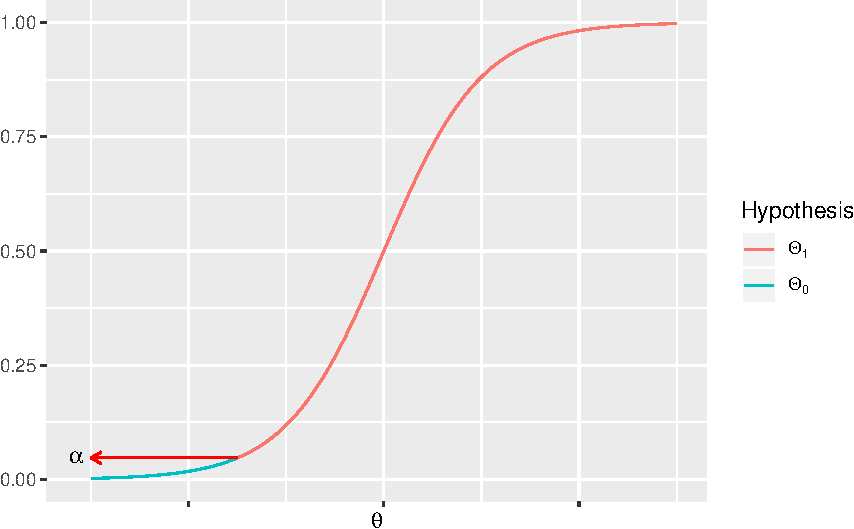
\includegraphics[width=0.7\linewidth]{statistical-computing_files/figure-latex/sizealpha-1} 

}

\caption{Size $\alpha$ Test}\label{fig:sizealpha}
\end{figure}

Then how to compare tests? Look at the following example. Three columns of the middle part are type I error rate.

\begin{longtable}[]{@{}ccccc@{}}
\toprule
test methods & \(\alpha = 0.01\) & \(\alpha = 0.05\) & \(\alpha = 0.01\) & Power\tabularnewline
\midrule
\endhead
Test 1 & 0.09 & 0.04 & 0.01 & 0.7\tabularnewline
Test 2 & 0.11 & 0.06 & 0.01 & 0.65\tabularnewline
Test 3 & 0.15 & 0.07 & 0.02 & 0.9\tabularnewline
\bottomrule
\end{longtable}

Here, we will choose \textbf{Test 1}.

\begin{enumerate}
\def\labelenumi{\arabic{enumi}.}
\tightlist
\item
  \(\text{Type I error rate} \approx \alpha\)

  \begin{itemize}
  \tightlist
  \item
    before looking at power, this should be satisfied.
  \item
    So Test 3 is excluded
  \end{itemize}
\item
  Larger power

  \begin{itemize}
  \tightlist
  \item
    Thus, we select Test 1.
  \end{itemize}
\end{enumerate}

\hypertarget{empirical-type-i-error-rate}{%
\subsection{Empirical type-I error rate}\label{empirical-type-i-error-rate}}

Recall Lemma \ref{lem:typeerr}. As in p-value, we just compute sample proportion for each type I error rate and power under null and alternative distribution.

\BeginKnitrBlock{lemma}
\protect\hypertarget{lem:testnull}{}{\label{lem:testnull} }Consider \(H_0: \theta \in \Theta_0 \qquad \text{vs} \qquad H_1: \theta \in \Theta_1\).

Define \(I(\mathbf{X})\) by

\[
I(\mathbf{X}) = \begin{cases}
  1 & H_0 \:\text{is rejected} \mid H_0 \\
  0 & otherwise
\end{cases}
\]

For each MC sample, compute this statistic \(I_m = I(\mathbf{X}^{m})\). Then empirical type I error rate can be computed as

\[\frac{1}{M}\sum_{m = 1}^M I_m\]
\EndKnitrBlock{lemma}

\begin{algorithm}[H] \label{alg:algtype1}
  \SetAlgoLined
  \SetKwInOut{Input}{input}
  \SetKwInOut{Output}{output}
  \Input{$H_0: \theta \in \Theta_0 \quad \text{vs} \quad H_1: \theta \in \Theta_1$}
  \For{$m \leftarrow 1$ \KwTo $M$}{
    Generate $X_1^{(m)}, \ldots, X_n^{(m)} \stackrel{H_0}{\sim}f$\; \label{alg:gentype1}
    Compute $T_m(\mathbf{X}^{(m)})$\;
    Compute $I_m = \begin{cases} 1 & H_0 \:\text{is rejected} \mid H_0 \\ 0 & \text{otherwise} \end{cases}$\;
  }
  Empirical Type I error rate $\hat\alpha = \frac{1}{M}\sum\limits_{m = 1}^M I_m$\;
  \Output{compare $\hat\alpha$ with $\alpha$}
  \caption{Empirical type I error rate by Monte Carlo method}
\end{algorithm}

\BeginKnitrBlock{example}[Testing normal mean]
\protect\hypertarget{exm:ttest}{}{\label{exm:ttest} \iffalse (Testing normal mean) \fi{} }Suppose that \(X_1, \ldots, X_{20} \stackrel{iid}{\sim}N(\mu, \sigma^2 = 100)\). Test

\[H_0: \mu = 500 \qquad \text{vs} \qquad H_1: \mu > 500\]

\begin{enumerate}
  \item $Z$-test: $Z = \frac{\overline{X} - 500}{\sigma^2 / \sqrt{20}} \stackrel{H_0}{\sim}N(0, 1)$
  \item $t$-test: $T = \frac{\overline{X} - 500}{S / \sqrt{20}} \stackrel{H_0}{\sim}t(20 - 1)$
\end{enumerate}
\EndKnitrBlock{example}

\begin{Shaded}
\begin{Highlighting}[]
\NormalTok{test_list <-}\StringTok{ }\ControlFlowTok{function}\NormalTok{(x, mu, sig, }\DataTypeTok{a =} \FloatTok{.05}\NormalTok{) \{}
\NormalTok{  n <-}\StringTok{ }\KeywordTok{length}\NormalTok{(x)}
\NormalTok{  xbar <-}\StringTok{ }\KeywordTok{mean}\NormalTok{(x) }\OperatorTok{-}\StringTok{ }\NormalTok{mu}
  \KeywordTok{list}\NormalTok{(}
    \DataTypeTok{z =}\NormalTok{ xbar }\OperatorTok{/}\StringTok{ }\NormalTok{(sig }\OperatorTok{/}\StringTok{ }\KeywordTok{sqrt}\NormalTok{(n)) }\OperatorTok{>}\StringTok{ }\KeywordTok{qnorm}\NormalTok{(a, }\DataTypeTok{lower.tail =} \OtherTok{FALSE}\NormalTok{),}
    \DataTypeTok{t =}\NormalTok{ xbar }\OperatorTok{/}\StringTok{ }\NormalTok{(}\KeywordTok{sd}\NormalTok{(x) }\OperatorTok{/}\StringTok{ }\KeywordTok{sqrt}\NormalTok{(n)) }\OperatorTok{>}\StringTok{ }\KeywordTok{qt}\NormalTok{(a, }\DataTypeTok{df =}\NormalTok{ n }\OperatorTok{-}\StringTok{ }\DecValTok{1}\NormalTok{, }\DataTypeTok{lower.tail =} \OtherTok{FALSE}\NormalTok{)}
\NormalTok{  )}
\NormalTok{\}}
\CommentTok{#--------------------}
\NormalTok{err_mc <-}
\StringTok{  }\KeywordTok{mc_data}\NormalTok{(rnorm, }\DataTypeTok{N =} \DecValTok{20}\NormalTok{, }\DataTypeTok{mean =} \DecValTok{500}\NormalTok{, }\DataTypeTok{sd =} \DecValTok{10}\NormalTok{)[,}
                                              \KeywordTok{lapply}\NormalTok{(.SD, test_list, }\DataTypeTok{mu =} \DecValTok{500}\NormalTok{, }\DataTypeTok{sig =} \DecValTok{10}\NormalTok{) }\OperatorTok\StringTok{ }
\StringTok{                                                }\KeywordTok{unlist}\NormalTok{() }\OperatorTok\StringTok{ }
\StringTok{                                                }\KeywordTok{as.list}\NormalTok{(),}
\NormalTok{                                              by =}\StringTok{ }\NormalTok{sam][,}
                                                        \KeywordTok{lapply}\NormalTok{(.SD, mean),}
\NormalTok{                                                        .SDcols =}\StringTok{ }\OperatorTok{-}\StringTok{"sam"}\NormalTok{]}
\end{Highlighting}
\end{Shaded}

\begin{table}[t]

\caption{\label{tab:errmc}Empirical Type I error for Z and T}
\centering
\begin{tabular}{r|r}
\hline
Z-test & T-test\\
\hline
0.048 & 0.051\\
\hline
\end{tabular}
\end{table}

Both test have Type I error close to \(\alpha\), but \(Z\)-test seems bit better.

\hypertarget{empirical-power}{%
\subsection{Empirical power}\label{empirical-power}}

Next step is power. See Figure \ref{fig:sizealpha}. Power is different in that this is computed in \emph{alternative distribution, not null distribution}.

\[\beta(\theta_1) = P(\text{reject}\: H_0 \mid \theta_1 \in \Theta_1)\]

\BeginKnitrBlock{lemma}
\protect\hypertarget{lem:testalt}{}{\label{lem:testalt} }Consider \(H_0: \theta \in \Theta_0 \qquad \text{vs} \qquad H_1: \theta \in \Theta_1\).

Define \(I(\mathbf{X})\) by

\[
I(\mathbf{X}) = \begin{cases}
  1 & H_0 \:\text{is rejected} \mid H_1 \\
  0 & otherwise
\end{cases}
\]

For each MC sample, compute this statistic \(I_m = I(\mathbf{X}^{m})\). Then empirical power can be computed as

\[\frac{1}{M}\sum_{m = 1}^M I_m\]
\EndKnitrBlock{lemma}

Process will be same but we test under \(H_1\). However, this makes a lot difference due to structure of each hypothesis. In many cases, \(H_0\) is simple, i.e.~\(\mu = 500\). In \(\ref{alg:gentype1}\) of Algorithm \(\ref{alg:algtype1}\), we can consider only \(N(\mu = 500, 100)\). Since \(\Theta_0\) and \(\Theta_1\) form partition, alternative hypothesis usually is not simple. In this example, \(\mu > 500\). We cannot specify one distribution for alternatrive. How to deal with this?

Trying many points for \(\mu_1 \in \Theta_1 = \{ \mu : \mu > 500 \}\) might be possible. Our goal is finding larger power. So \emph{find test with larger power for all points in} \(\Theta_1\).

\begin{figure}[H]

{\centering 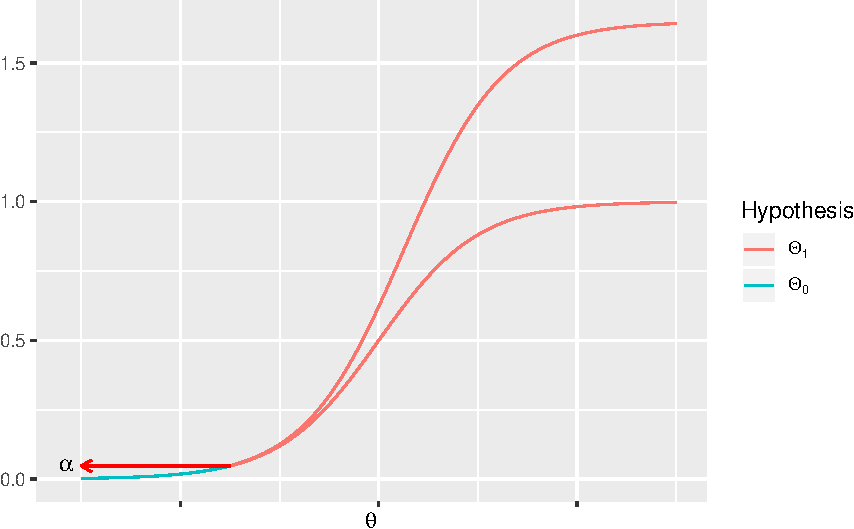
\includegraphics[width=0.7\linewidth]{statistical-computing_files/figure-latex/powercomp-1} 

}

\caption{Comparing power between two test methods}\label{fig:powercomp}
\end{figure}

See Figure \ref{fig:powercomp}. One test method has higher \(\beta(\theta)\) function curve in \(\Theta_1\). This test is \emph{powerful than the other}. We would choose this test in this step. So what we have to do is choose some points \(\theta_1 \in \Theta_1\), and draw the power curve.

\begin{algorithm}[H] \label{alg:algpower}
  \SetAlgoLined
  \SetKwInOut{Input}{input}
  \SetKwInOut{Output}{output}
  \Input{$H_0: \theta \in \Theta_0 \quad \text{vs} \quad H_1: \theta \in \Theta_1$}
  \ForEach{$\theta_1 \in \Theta_1$}{
    \For{$m \leftarrow 1$ \KwTo $M$}{
      Generate $X_1^{(m)}, \ldots, X_n^{(m)} \stackrel{H_0}{\sim}f$\;
      Compute $T_m(\mathbf{X}^{(m)})$\;
      Compute $I_m = \begin{cases} 1 & H_0 \:\text{is rejected} \mid H_1 \\ 0 & \text{otherwise} \end{cases}$\;
    }
    Empirical power $\hat\beta = \frac{1}{M}\sum\limits_{m = 1}^M I_m$\;
  }
  Draw a power curve $\hat\beta$ against $\theta_1$
  \Output{curve and $\{ \hat\beta \}$}
  \caption{Empirical power by Monte Carlo method}
\end{algorithm}

In fact, we can try every \(\theta \in \Theta\) and \emph{draw entire power curve}. Refer to Example \ref{exm:ttest}.

\begin{Shaded}
\begin{Highlighting}[]
\NormalTok{pw_mc <-}
\StringTok{  }\KeywordTok{lapply}\NormalTok{(}\KeywordTok{seq}\NormalTok{(}\DecValTok{450}\NormalTok{, }\DecValTok{650}\NormalTok{, }\DataTypeTok{by =} \DecValTok{10}\NormalTok{), }\ControlFlowTok{function}\NormalTok{(mu) \{}
    \KeywordTok{mc_data}\NormalTok{(rnorm, }\DataTypeTok{N =} \DecValTok{20}\NormalTok{, }\DataTypeTok{mean =}\NormalTok{ mu, }\DataTypeTok{sd =} \DecValTok{10}\NormalTok{)[,}
\NormalTok{                                               h1 }\OperatorTok{:}\ErrorTok{=}\StringTok{ }\NormalTok{mu]}
\NormalTok{  \})}
\NormalTok{pw_mc <-}\StringTok{ }\KeywordTok{rbindlist}\NormalTok{(pw_mc)}
\end{Highlighting}
\end{Shaded}

One column is added from previous process. This is group for \(H_1\). So we should specify \texttt{by\ =\ .(h1,\ sam)}.

\begin{Shaded}
\begin{Highlighting}[]
\NormalTok{pw_mc <-}
\StringTok{  }\NormalTok{pw_mc[,}
        \KeywordTok{lapply}\NormalTok{(.SD, test_list, }\DataTypeTok{mu =} \DecValTok{500}\NormalTok{, }\DataTypeTok{sig =} \DecValTok{10}\NormalTok{) }\OperatorTok\StringTok{ }
\StringTok{          }\KeywordTok{unlist}\NormalTok{() }\OperatorTok\StringTok{ }
\StringTok{          }\KeywordTok{as.list}\NormalTok{(),}
\NormalTok{        by =}\StringTok{ }\NormalTok{.(h1, sam)][,}
                         \KeywordTok{lapply}\NormalTok{(.SD, mean),}
\NormalTok{                         by =}\StringTok{ }\NormalTok{h1, .SDcols =}\StringTok{ }\OperatorTok{-}\StringTok{"sam"}\NormalTok{]}
\end{Highlighting}
\end{Shaded}

\begin{Shaded}
\begin{Highlighting}[]
\NormalTok{pw_mc }\OperatorTok\StringTok{ }
\StringTok{  }\KeywordTok{melt}\NormalTok{(}\DataTypeTok{id.vars =} \StringTok{"h1"}\NormalTok{, }\DataTypeTok{variable.name =} \StringTok{"test"}\NormalTok{) }\OperatorTok\StringTok{ }
\StringTok{  }\KeywordTok{ggplot}\NormalTok{(}\KeywordTok{aes}\NormalTok{(}\DataTypeTok{x =}\NormalTok{ h1, }\DataTypeTok{y =}\NormalTok{ value, }\DataTypeTok{colour =}\NormalTok{ test)) }\OperatorTok{+}
\StringTok{  }\KeywordTok{geom_path}\NormalTok{() }\OperatorTok{+}
\StringTok{  }\KeywordTok{geom_point}\NormalTok{() }\OperatorTok{+}
\StringTok{  }\KeywordTok{scale_colour_discrete}\NormalTok{(}
    \DataTypeTok{name =} \StringTok{"Test"}\NormalTok{,}
    \DataTypeTok{labels =} \KeywordTok{c}\NormalTok{(}\StringTok{"Z"}\NormalTok{, }\StringTok{"T"}\NormalTok{)}
\NormalTok{  ) }\OperatorTok{+}
\StringTok{  }\KeywordTok{labs}\NormalTok{(}
    \DataTypeTok{x =} \KeywordTok{expression}\NormalTok{(mu),}
    \DataTypeTok{y =} \KeywordTok{expression}\NormalTok{(beta)}
\NormalTok{  )}
\end{Highlighting}
\end{Shaded}

\begin{figure}[H]

{\centering 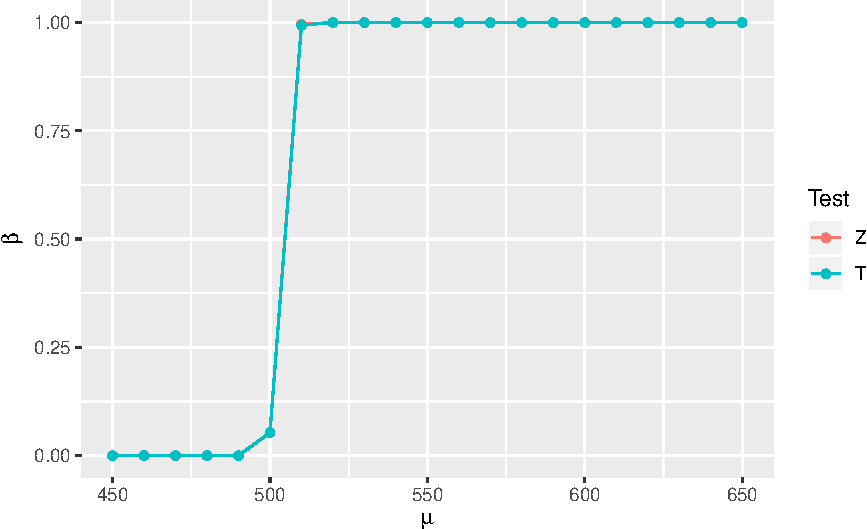
\includegraphics[width=0.7\linewidth]{statistical-computing_files/figure-latex/mupwcurve-1} 

}

\caption{Empirical power curve of each z-test and t-test}\label{fig:mupwcurve}
\end{figure}

Recall that we are estimating power. Instead of \texttt{mean()}, we can use \texttt{sd()}. This would give us \emph{standard error} of our estimator for power. Since it is sample proportion,

\[\widehat{SE}(\hat{p}) = \sqrt{\frac{\hat{p}(1 - \hat{p})}{M}}\]

Consider \(T\)-test.

\begin{Shaded}
\begin{Highlighting}[]
\NormalTok{pw_mc2 <-}\StringTok{ }\KeywordTok{lapply}\NormalTok{(}\KeywordTok{seq}\NormalTok{(}\DecValTok{450}\NormalTok{, }\DecValTok{650}\NormalTok{, }\DataTypeTok{by =} \DecValTok{10}\NormalTok{), }\ControlFlowTok{function}\NormalTok{(mu) \{}
  \KeywordTok{mc_data}\NormalTok{(rnorm, }\DataTypeTok{N =} \DecValTok{20}\NormalTok{, }\DataTypeTok{mean =}\NormalTok{ mu, }\DataTypeTok{sd =} \DecValTok{10}\NormalTok{)[,}
\NormalTok{                                             h1 }\OperatorTok{:}\ErrorTok{=}\StringTok{ }\NormalTok{mu]}
\NormalTok{\})}
\NormalTok{pw_mc2 <-}\StringTok{ }\KeywordTok{rbindlist}\NormalTok{(pw_mc2)}
\CommentTok{#------------------}
\NormalTok{pw_mc2 <-}
\StringTok{  }\NormalTok{pw_mc2[,}
\NormalTok{         .(}\DataTypeTok{te =} \KeywordTok{t.test}\NormalTok{(x, }\DataTypeTok{alternative =} \StringTok{"greater"}\NormalTok{, }\DataTypeTok{mu =} \DecValTok{500}\NormalTok{)}\OperatorTok{$}\NormalTok{p.value }\OperatorTok{<=}\StringTok{ }\FloatTok{.05}\NormalTok{),}
\NormalTok{         by =}\StringTok{ }\NormalTok{.(h1, sam)][,}
\NormalTok{                          .(}\DataTypeTok{te =} \KeywordTok{mean}\NormalTok{(te)),}
\NormalTok{                          by =}\StringTok{ }\NormalTok{h1][,}
\NormalTok{                                   se }\OperatorTok{:}\ErrorTok{=}\StringTok{ }\KeywordTok{sqrt}\NormalTok{(te }\OperatorTok{*}\StringTok{ }\NormalTok{(}\DecValTok{1} \OperatorTok{-}\StringTok{ }\NormalTok{te) }\OperatorTok{/}\StringTok{ }\DecValTok{1000}\NormalTok{)]}
\end{Highlighting}
\end{Shaded}

\begin{Shaded}
\begin{Highlighting}[]
\NormalTok{pw_mc2 }\OperatorTok\StringTok{ }
\StringTok{  }\KeywordTok{ggplot}\NormalTok{(}\KeywordTok{aes}\NormalTok{(}\DataTypeTok{x =}\NormalTok{ h1, }\DataTypeTok{y =}\NormalTok{ te)) }\OperatorTok{+}
\StringTok{  }\KeywordTok{geom_ribbon}\NormalTok{(}\KeywordTok{aes}\NormalTok{(}\DataTypeTok{ymin =}\NormalTok{ te }\OperatorTok{-}\StringTok{ }\NormalTok{se, }\DataTypeTok{ymax =}\NormalTok{ te }\OperatorTok{+}\StringTok{ }\NormalTok{se), }\DataTypeTok{col =} \KeywordTok{gg_hcl}\NormalTok{(}\DecValTok{1}\NormalTok{)) }\OperatorTok{+}
\StringTok{  }\KeywordTok{geom_path}\NormalTok{(}\DataTypeTok{alpha =} \FloatTok{.7}\NormalTok{) }\OperatorTok{+}
\StringTok{  }\KeywordTok{geom_point}\NormalTok{() }\OperatorTok{+}
\StringTok{  }\KeywordTok{labs}\NormalTok{(}
    \DataTypeTok{x =} \KeywordTok{expression}\NormalTok{(mu),}
    \DataTypeTok{y =} \KeywordTok{expression}\NormalTok{(beta)}
\NormalTok{  )}
\end{Highlighting}
\end{Shaded}

\begin{figure}[H]

{\centering 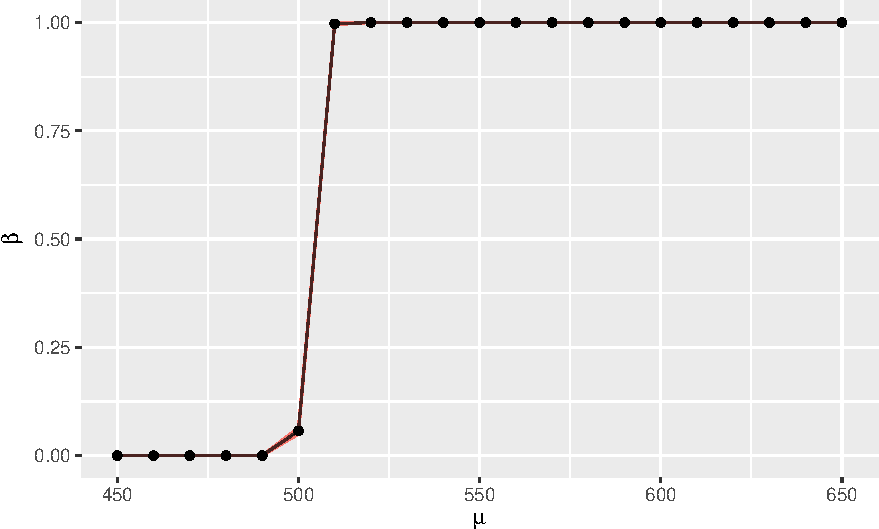
\includegraphics[width=0.7\linewidth]{statistical-computing_files/figure-latex/pwse-1} 

}

\caption{Empirical power curve $\hat{p} \pm \widehat{SE}(\hat{p})$ for t-test}\label{fig:pwse}
\end{figure}

\hypertarget{count-five-test-for-equal-variance}{%
\subsection{Count Five test for equal variance}\label{count-five-test-for-equal-variance}}

Commonly, F-test is used for equality of two population variances. \citet{McGrath:2005kx} suggests nonparametric testing without Normal assumption, so called \emph{Count Five}. Instead, this method requires some conditions.

\begin{enumerate}
\def\labelenumi{\arabic{enumi}.}
\tightlist
\item
  same mean
\item
  same sample size
\end{enumerate}

\begin{algorithm}[H] \label{alg:algcfive}
  \SetAlgoLined
  \SetKwInOut{Input}{input}
  \SetKwInOut{Output}{output}
  \Input{$X_1, \ldots, X_{n_x} \perp\!\!\!\perp Y_1, \ldots, Y_{n_y}$ \\ $H_0: \sigma_X^2 = \sigma_Y^2$}
  Compute $C_X = \Big\lvert \{ i : \lvert X_i - \overline{X} \rvert > \max_j \lvert Y_j - \overline{Y} \rvert \} \Big\rvert$\;
  \uIf{$C_X \ge 5$}{
    \Return reject $H_0$\;
  }
  \Else{
    \Return accept $H_0$\;
  }
  \caption{Count Five test}
\end{algorithm}

\begin{Shaded}
\begin{Highlighting}[]
\NormalTok{gauss <-}
\StringTok{  }\KeywordTok{tibble}\NormalTok{(}
    \DataTypeTok{x1 =} \KeywordTok{rnorm}\NormalTok{(}\DecValTok{20}\NormalTok{, }\DataTypeTok{mean =} \DecValTok{0}\NormalTok{, }\DataTypeTok{sd =} \DecValTok{1}\NormalTok{),}
    \DataTypeTok{x2 =} \KeywordTok{rnorm}\NormalTok{(}\DecValTok{20}\NormalTok{, }\DataTypeTok{mean =} \DecValTok{0}\NormalTok{, }\DataTypeTok{sd =} \FloatTok{1.5}\NormalTok{)}
\NormalTok{  )}
\end{Highlighting}
\end{Shaded}

\begin{Shaded}
\begin{Highlighting}[]
\NormalTok{gauss }\OperatorTok\StringTok{ }
\StringTok{  }\KeywordTok{gather}\NormalTok{(}\DataTypeTok{key =} \StringTok{"variable"}\NormalTok{, }\DataTypeTok{value =} \StringTok{"value"}\NormalTok{) }\OperatorTok\StringTok{ }
\StringTok{  }\KeywordTok{ggplot}\NormalTok{(}\KeywordTok{aes}\NormalTok{(}\DataTypeTok{x =}\NormalTok{ variable, }\DataTypeTok{y =}\NormalTok{ value, }\DataTypeTok{fill =}\NormalTok{ variable)) }\OperatorTok{+}
\StringTok{  }\KeywordTok{geom_boxplot}\NormalTok{() }\OperatorTok{+}
\StringTok{  }\KeywordTok{geom_point}\NormalTok{(}\DataTypeTok{alpha =} \FloatTok{.5}\NormalTok{)}
\end{Highlighting}
\end{Shaded}

\begin{figure}[H]

{\centering 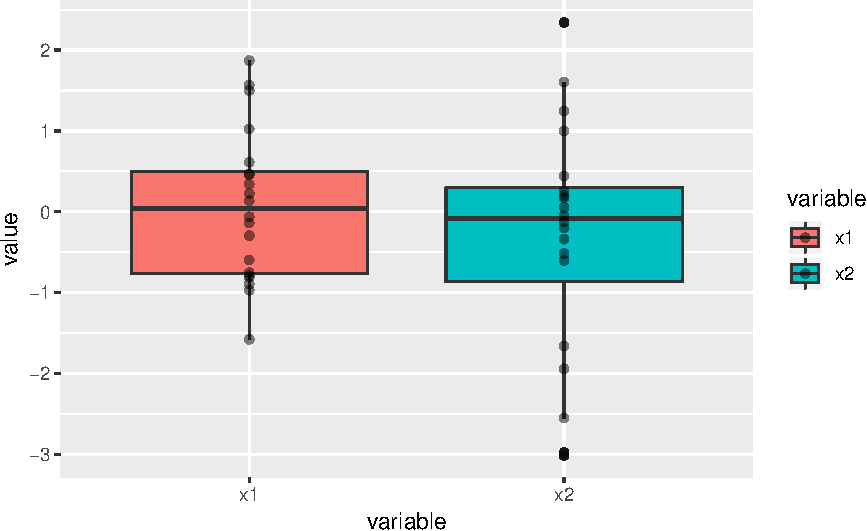
\includegraphics[width=0.7\linewidth]{statistical-computing_files/figure-latex/sigbox-1} 

}

\caption{Side-by-side boxplot}\label{fig:sigbox}
\end{figure}

We would perform \emph{Count Five} test for multiple simulated data sets such as in Figure \ref{fig:sigbox}.

\[X_1^{(m)}, \ldots, X_{20}^{(m)} \sim N(0, 1) \perp\!\!\!\perp Y_1^{(m)}, \ldots, Y_{20}^{(m)} \sim N(0, 1.5)\]

\begin{Shaded}
\begin{Highlighting}[]
\NormalTok{count5test <-}\StringTok{ }\ControlFlowTok{function}\NormalTok{(x, y) \{}
\NormalTok{  X <-}\StringTok{ }\NormalTok{x }\OperatorTok{-}\StringTok{ }\KeywordTok{mean}\NormalTok{(x)}
\NormalTok{  Y <-}\StringTok{ }\NormalTok{x }\OperatorTok{-}\StringTok{ }\KeywordTok{mean}\NormalTok{(y)}
\NormalTok{  outx <-}\StringTok{ }\KeywordTok{sum}\NormalTok{(X }\OperatorTok{>}\StringTok{ }\KeywordTok{max}\NormalTok{(Y)) }\OperatorTok{+}\StringTok{ }\KeywordTok{sum}\NormalTok{(X }\OperatorTok{<}\StringTok{ }\KeywordTok{min}\NormalTok{(Y))}
\NormalTok{  outy <-}\StringTok{ }\KeywordTok{sum}\NormalTok{(Y }\OperatorTok{>}\StringTok{ }\KeywordTok{max}\NormalTok{(X)) }\OperatorTok{+}\StringTok{ }\KeywordTok{sum}\NormalTok{(Y }\OperatorTok{<}\StringTok{ }\KeywordTok{min}\NormalTok{(X))}
  \KeywordTok{max}\NormalTok{(}\KeywordTok{c}\NormalTok{(outx, outy)) }\OperatorTok{>}\StringTok{ }\DecValTok{5}
\NormalTok{\}}
\end{Highlighting}
\end{Shaded}

Apply MC method to get \emph{empirical type I error}.

\begin{Shaded}
\begin{Highlighting}[]
\KeywordTok{mc_data}\NormalTok{(rnorm, }\DataTypeTok{N =} \DecValTok{20}\NormalTok{, }\DataTypeTok{M =} \DecValTok{1000}\NormalTok{)[,}
\NormalTok{                                 x2 }\OperatorTok{:}\ErrorTok{=}\StringTok{ }\KeywordTok{rnorm}\NormalTok{(}\DecValTok{20} \OperatorTok{*}\StringTok{ }\DecValTok{1000}\NormalTok{)][,}
\NormalTok{                                                         .(}\DataTypeTok{chat =} \KeywordTok{count5test}\NormalTok{(}\DataTypeTok{x =}\NormalTok{ x, }\DataTypeTok{y =}\NormalTok{ x2)),}
\NormalTok{                                                         by =}\StringTok{ }\NormalTok{sam][,}
\NormalTok{                                                                   .(}\DataTypeTok{chat =} \KeywordTok{mean}\NormalTok{(chat))]}
\CommentTok{#>     chat}
\CommentTok{#> 1: 0.026}
\end{Highlighting}
\end{Shaded}

\hypertarget{statistical-methods}{%
\section{Statistical Methods}\label{statistical-methods}}

\hypertarget{bootstrap}{%
\section{Bootstrap}\label{bootstrap}}

\hypertarget{resampling}{%
\subsection{Resampling}\label{resampling}}

Bootstrap is a class of nonparametric Monte Carlo methods that estimate the distribution of a population by \emph{resampling}. Different with previous MC method, we do not know population distribution. Instead, resampling methods treat an observed sample as a finte population. This is called \emph{pseudo-population} in that this is regarded as having the same characteristics as the true population.

\begin{figure}[H]

{\centering 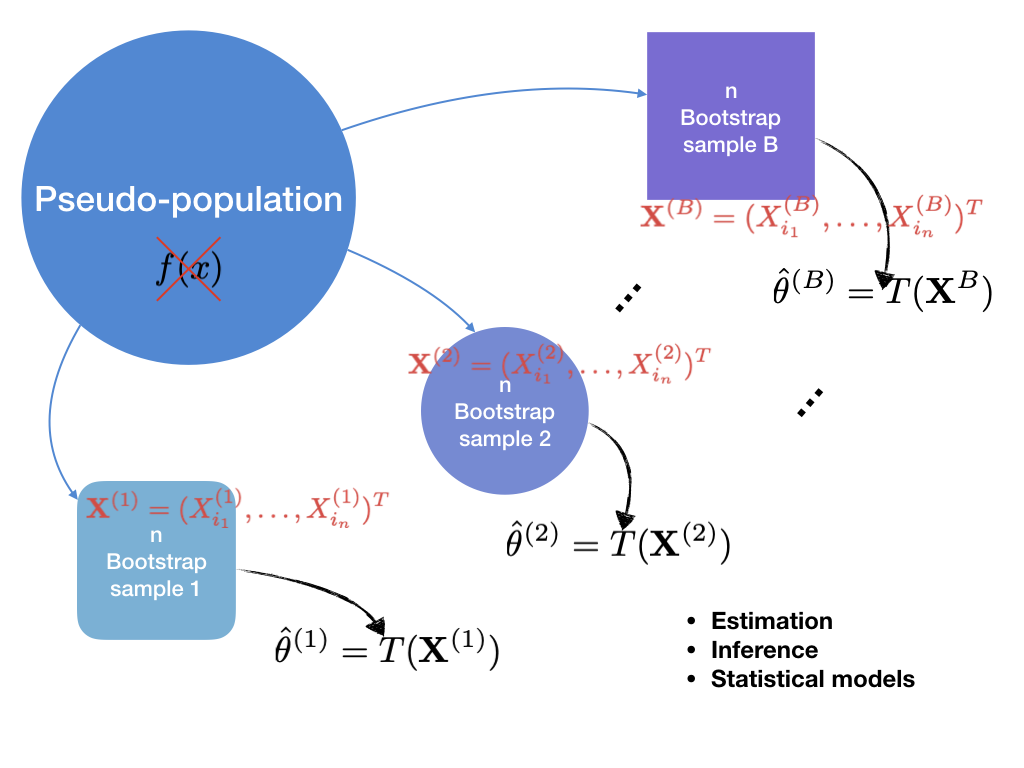
\includegraphics[width=0.7\linewidth]{images/resample} 

}

\caption{Resampling}\label{fig:resample}
\end{figure}

See Figure \ref{fig:resample}. From the observed sample, which is pseudo-population, resampling generates multiple bootstrap samples by \emph{sampling with replacement}. Surprisingly, this simple sampling procedure approximate the true population distribution quite successful.

\hypertarget{bootapprox}{%
\subsection{Approximations in bootstrap}\label{bootapprox}}

How does bootstrap work? \citet{Efron:1983bw} provides simple example \(T = \overline{x}\), i.e.~sample average.

\BeginKnitrBlock{example}[Estimation of sample mean]
\protect\hypertarget{exm:bootave}{}{\label{exm:bootave} \iffalse (Estimation of sample mean) \fi{} }Having observed \(X_1 = x_1, \ldots, X_n = x_n\), compute

\[\overline{x} = \frac{1}{n} \sum_{i = 1}^n x_i\]

Using bootstrap, we try to see the empirical distribution of this.
\EndKnitrBlock{example}

Note that

\[X_1, \ldots, X_n \stackrel{iid}{\sim}F\]

where \(F\) is true unknown distribution. Having observed \(X_1 = x_1, \ldots, X_n = x_n\), we get \emph{empirical distribution function} by computing the sample average.

\begin{equation}
  \hat{F}(x) = \frac{1}{n} \sum_{i = 1}^n I(X_i \le x_i)
  \label{eq:edistn}
\end{equation}

This works for estimator of \(F\). \(\hat{F}\) endows mass \(\frac{1}{n}\) on each observed point \(x_i, \: i = 1, \ldots, n\). In other words, pseudo-distribution becomes \emph{discrete uniform}.

\begin{equation}
  \hat{F} \stackrel{d}{=} unif(x_1, \ldots, x_n)
  \label{eq:discunif}
\end{equation}

We have set the population distribution which is bogus. Now we can apply previous MC sampling with \(\frac{1}{n}\). Write \(\{ X_1^{\ast}, \ldots, X_n^{\ast} \}\) as \emph{bootstrap sample} by resampling. Then

\[P(X^{\ast} = x_i) = \frac{1}{n}\]

i.e.

\begin{equation}
  X^{\ast} \stackrel{iid}{\sim}unif(x_1, \ldots, x_n)
  \label{eq:bootdistn}
\end{equation}

This gives \emph{bootstrap cdf}, cdf of bootstrap samples, by

\begin{equation}
  F^{\ast}(x) = \text{cdf of}\: unif(x_1, \ldots, x_n) = \hat{F}
  \label{eq:bootcdf}
\end{equation}

One proceeds in a similar way for estimating cdf that

\begin{equation}
  \hat{F}^{\ast} = \frac{1}{n} \sum_{i = 1}^n I(X^{\ast} \le x_i)
  \label{eq:bootecdf}
\end{equation}

This is called \emph{ecdf of bootstrap replicates}.

\BeginKnitrBlock{remark}
\iffalse{} {Remark. } \fi{}For any data points \(X_1, \ldots, X_n\),

\begin{enumerate}
  \item \textbf{\textit{Empirical Distribution Function}} $\hat{F}(x) = \frac{1}{n} \sum_{i = 1}^n I(X_i \le x_i)$
  \item \textbf{\textit{Bootstrap cdf}} $F^{\ast}(x) = \hat{F}$
  \item \textbf{\textit{ECDF of bootstrap replicates}} $\hat{F}^{\ast} = \frac{1}{n} \sum_{i = 1}^n I(X^{\ast} \le x_i)$
\end{enumerate}
\EndKnitrBlock{remark}

This remark can explain Figure \ref{fig:resample} in a distribution way.

\begin{figure}[H]

{\centering 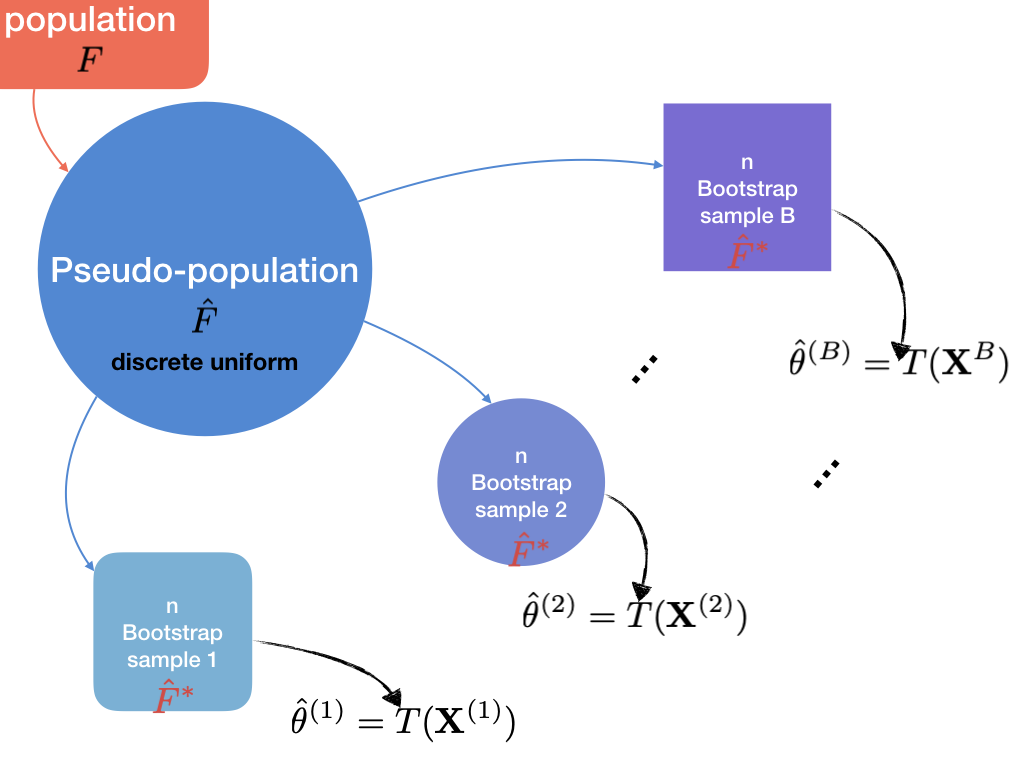
\includegraphics[width=0.7\linewidth]{images/bootapprox} 

}

\caption{Empirical distribution of bootstrap}\label{fig:bootapprox}
\end{figure}

Figure \ref{fig:bootapprox} shows how each sample is distributed, approximately. We get the data set from true \(F\). From this finite population, we first estimate \(F\) by \(\hat{F}\). Resampling multiple bootstrap samples, each sample estimates \(\hat{F}\) by \(\hat{F}^{\ast}\).

\BeginKnitrBlock{theorem}[Two approximations in bootstrap]
\protect\hypertarget{thm:twoapprox}{}{\label{thm:twoapprox} \iffalse (Two approximations in bootstrap) \fi{} }There are two approximations in bootstrap. For large \(B\), bootstrap samples approximate bootstrap replicates. For large \(n\), bootstrap replicates approximate true population.

\[\mathbf{X}^{(b)} \vertarrowbox[3ex]{\rightarrow}{\text{large}\: B} \hat{f} \vertarrowbox{\rightarrow}{\text{large}\: n} f\]
\EndKnitrBlock{theorem}

\BeginKnitrBlock{proof}
\iffalse{} {Proof. } \fi{}Since

\[E\hat{F} = \frac{1}{n} \sum_{i = 1}^n P(X_i \le x_i)\]

\[\hat{F} \stackrel{a.s.}{\rightarrow} F\]

as \(n \rightarrow \infty\) by the strong law of large numbers. Let

\[\overline{\hat{F}^{\ast}} := \frac{1}{B} \sum_b \hat{F}_b^{\ast}\]

where \(\hat{F}_b^{\ast}\) is ecdf of \(b\)-th bootstrap replicate. Since

\[E\hat{F}_b^{\ast} = \frac{1}{n} \sum_{i = 1}^n P(X^{(b)} \le x_i)\]

\[\overline{\hat{F}^{\ast}} \stackrel{a.s.}{\rightarrow} F^{\ast} = \hat{F}\]

as \(B \rightarrow \infty\) by S.L.L.N.
\EndKnitrBlock{proof}

Denote that Theorem \ref{thm:twoapprox} can be also expressed as

\begin{equation}
  \overline{\hat{F}^{\ast}} \vertarrowbox[3ex]{\rightarrow}{\text{large}\: B} \hat{F} \vertarrowbox{\rightarrow}{\text{large}\: n} F
  \label{eq:twoapprox2}
\end{equation}

This approximation not only justifies the bootstrap procedure but also shows the problem of it. We can always increase \(B\) if we want. Then we earn \(\overline{\hat{F}^{\ast}} \approx \hat{F}\), i.e.~bootstrap samples approximate pseudo-population. However, \(n\) is fixed. For \(\hat{F}\) to approximate \(F\), large \(n\) is required. It is not under control. If small \(n\) is given, \(\hat{F}\) will not be close to \(F\). Then the bootstrap samples will not be close to \(F\) finally.

\BeginKnitrBlock{corollary}
\protect\hypertarget{cor:bootprob}{}{\label{cor:bootprob} }Resampling the large number of replicates, i.e.~large \(B\) produces a good estimates of \(\hat{F}\) but it does not guarantee a good estimate of \(F\).
\EndKnitrBlock{corollary}

\BeginKnitrBlock{example}[Poisson population]
\protect\hypertarget{exm:bootpois}{}{\label{exm:bootpois} \iffalse (Poisson population) \fi{} }Suppose that \(\{ 2, 2, 1, 1, 5, 4, 4, 3, 2, 1 \} \sim Poisson(\lambda = 2)\). Resampling from this pseudo-population, can we appropriately explain the population?
\EndKnitrBlock{example}

\begin{longtable}{r|r|r|r|r}
\caption{\label{tab:bootpoisemp}Empirical distribution}\\
\hline
1 & 2 & 3 & 4 & 5\\
\hline
0.3 & 0.3 & 0.1 & 0.2 & 0.1\\
\hline
\end{longtable}

Table \(\ref{tab:bootpoisemp}\) is just a result of averaging, emprical distribution \(\hat{F}\). General bootstrap will resample by distribution. We can see the problem at once.

\[P(X = 0) = e^{-2} = 0.135\]

However, we did not observe \(0\), so the bootstrap sample will never include zero, i.e.~not a full domain. In sum,

\[\overline{\hat{F}^{\ast}} \rightarrow \hat{F} {\color{red}{\not}}{\rightarrow} F\]

\hypertarget{bootstrap-standard-error}{%
\subsection{Bootstrap standard error}\label{bootstrap-standard-error}}

Look at the Figure \ref{fig:bootapprox} again. For each sample, we calculate esimator of our interest. For instance, Example \ref{exm:bootave} - sample average \(\overline{x}\). After that, we get empirical distribution of \(\overline{x}\) such as \emph{standard error}.

Before looking at the empirical distribution, let's review sample estimation.

\BeginKnitrBlock{theorem}[Standard error of sample mean]
\protect\hypertarget{thm:samplemean}{}{\label{thm:samplemean} \iffalse (Standard error of sample mean) \fi{} }Standard error of \(\overline{X} = \overline{x} = \frac{1}{n} \displaystyle\sum_{i = 1}^n x_i\), i.e.~the \textit{root mean squred error} is estimated by

\[\hat\sigma = \bigg[ \frac{1}{n (n - 1)} \sum_{i = 1}^n (x_i - \overline{x})^2 \bigg]^{\frac{1}{2}}\]
\EndKnitrBlock{theorem}

Here, \(n - 1\) was divided for \emph{unbiasedness}. Recall that

\[Var(\overline{X}) = \frac{\sigma^2}{n}\]

It follows that

\[\hat\sigma^2 = \frac{s^2}{n}\]

and we know that \(s^2\) should be divided by \(n - 1\) to be unbiased. Bootstrap generalizes point estimation process \ref{thm:samplemean} a bit differently \citep{Efron:1983bw}. From Equation \eqref{eq:edistn} to \eqref{eq:bootcdf}, we resample bootstrap sample with empricial probability distribution \(\hat{F}\) so that

\begin{equation}
  X_1^{\ast}, \ldots, X_n^{\ast} \stackrel{iid}{\sim}\hat{F}
  \label{eq:samplescheme}
\end{equation}

where \(\hat{F}\) is discrete uniform in each observed data point. In this sample, compute the estimate of interest, e.g.~average

\[\overline{X}^{\ast} = \frac{1}{n} \sum_{i = 1}^n X_i^{\ast}\]

From Theorem \ref{thm:samplemean}, this \(\overline{X}^{\ast}\) has \emph{estimated variance} of

\begin{equation}
  Var\overline{X}^{\ast} = \frac{1}{n(n - 1)} \sum_{i = 1}^n (X_i - \overline{X})^2
  \label{eq:varundersam}
\end{equation}

In fact, this is a variance \emph{under sampling scheme} \eqref{eq:samplescheme}, i.e.~indicates one-time-sampling from \(\hat{F}\). Using this, we can construct \textbf{bootstrap estimate of standard error for sample mean}, which come by sampling \(B\) times.

\begin{equation}
  \hat\sigma_B = \bigg[ \frac{1}{B - 1} \sum_{b = 1}^B (\overline{X}_b^{\ast} - \overline{X}_{.}^{\ast})^2 \bigg]^{\frac{1}{2}}
  \label{eq:sebootave}
\end{equation}

where \(\overline{X}_b^{\ast}\) is a sample mean of \(b\)-th bootstrap replicate and \(\overline{X}_{.}^{\ast}\) is average of every \(\overline{X}_b^{\ast}\).

\BeginKnitrBlock{theorem}[Bootstrap standard error]
\protect\hypertarget{thm:bootse}{}{\label{thm:bootse} \iffalse (Bootstrap standard error) \fi{} }Bootstrap estimate of standard error for any estimator \(\hat\theta(X_1, \ldots, X_n)\) is

\[\hat\sigma_B = \bigg[ \frac{1}{B - 1} \sum_{b = 1}^B (\hat\theta_b^{\ast} - \overline{\hat\theta^{\ast}})^2 \bigg]^{\frac{1}{2}}\]

where \(\hat\theta_b^{\ast}\) is independent bootstrap replications and

\[\overline{\hat\theta^{\ast}} = \frac{1}{B} \sum_{b = 1}^B \hat\theta_b^{\ast}\]
\EndKnitrBlock{theorem}

Now we format Figure \ref{fig:bootapprox} to practical algorithm.

\begin{algorithm}[H] \label{alg:algboot}
  \SetAlgoLined
  \SetKwInOut{Input}{input}
  \SetKwInOut{Output}{output}
  \KwData{$n$ observations $x_1, \ldots, x_n$}
  \Input{statistic of interest $\hat\theta$, the number of bootstrap replicates $B$}
  \For{$b \leftarrow 1$ \KwTo $B$}{
    Sampling with replacement $X_{1}^{(b)}, \ldots, X_n^{(b)}$ from the observed sample\;
    Compute estimate $$\hat\theta(X_{1}^{(b)}, \ldots, X_n^{(b)}) \equiv \hat\theta_b^{\ast}$$\;
  }
  $\overline{\hat\theta^{\ast}} = \frac{1}{B} \sum\limits_{b = 1}^B \hat\theta_b^{\ast}$\;
  Bootsrap standard error $$\hat\sigma_B = \bigg[ \frac{1}{B - 1} \sum_{b = 1}^B (\hat\theta_b^{\ast} - \overline{\hat\theta^{\ast}})^2 \bigg]^{\frac{1}{2}}$$\;
  \Output{$\hat\sigma_B$}
  \caption{Bootstrap algorithm}
\end{algorithm}

\citet{Efron:1994aa} suggests that \(B = 40\) is usually enough to estimate standard error well. It rarely require \(B > 200\). On the other hand, much larger \(B\) is needed in interval estimation.

First we try perform bootstrap without package doing bootstrap such as \texttt{boot} or \texttt{bootstrap}. The following is observed sample \(n = 50\), i.e.~finite population in bootstrap literature.

\begin{Shaded}
\begin{Highlighting}[]
\NormalTok{X}
\CommentTok{#> # A tibble: 50 x 1}
\CommentTok{#>        x}
\CommentTok{#>    <dbl>}
\CommentTok{#>  1 35.2 }
\CommentTok{#>  2  3.24}
\CommentTok{#>  3 11.5 }
\CommentTok{#>  4  6.00}
\CommentTok{#>  5 48.9 }
\CommentTok{#>  6  2.71}
\CommentTok{#>  7 38.7 }
\CommentTok{#>  8 34.0 }
\CommentTok{#>  9 19.8 }
\CommentTok{#> 10 40.8 }
\CommentTok{#> # ... with 40 more rows}
\end{Highlighting}
\end{Shaded}

Sample mean of this sample is

\begin{Shaded}
\begin{Highlighting}[]
\NormalTok{X }\OperatorTok\StringTok{ }
\StringTok{  }\KeywordTok{summarise}\NormalTok{(}\DataTypeTok{x =} \KeywordTok{mean}\NormalTok{(x))}
\CommentTok{#> # A tibble: 1 x 1}
\CommentTok{#>       x}
\CommentTok{#>   <dbl>}
\CommentTok{#> 1  22.2}
\end{Highlighting}
\end{Shaded}

\begin{Shaded}
\begin{Highlighting}[]
\NormalTok{MC_CORES <-}\StringTok{ }\NormalTok{parallel}\OperatorTok{::}\KeywordTok{detectCores}\NormalTok{() }\OperatorTok{-}\StringTok{ }\DecValTok{1} \CommentTok{# parallelization}
\end{Highlighting}
\end{Shaded}

\begin{Shaded}
\begin{Highlighting}[]
\NormalTok{resample <-}\StringTok{ }\ControlFlowTok{function}\NormalTok{(data, }\DataTypeTok{statistic =}\NormalTok{ mean) \{}
  \CommentTok{# sampling with replacement}
\NormalTok{  xb <-}
\StringTok{    }\NormalTok{data }\OperatorTok\StringTok{ }
\StringTok{    }\KeywordTok{data.table}\NormalTok{() }\OperatorTok\StringTok{ }
\StringTok{    }\NormalTok{.[}\KeywordTok{sample}\NormalTok{(}\DecValTok{1}\OperatorTok{:}\NormalTok{.N, }\DataTypeTok{size =}\NormalTok{ .N, }\DataTypeTok{replace =} \OtherTok{TRUE}\NormalTok{)]}
  \CommentTok{# estimator}
\NormalTok{  xb[,}
     \KeywordTok{lapply}\NormalTok{(.SD, statistic)] }\OperatorTok\StringTok{ }
\StringTok{    }\KeywordTok{as.numeric}\NormalTok{()}
\NormalTok{\}}
\end{Highlighting}
\end{Shaded}

To fasten the process, we implement parallization \texttt{parallel::mclapply}. This function is based on fork mechanism of Unix OS. So this is not available in Windows OS.

\begin{Shaded}
\begin{Highlighting}[]
\NormalTok{B <-}\StringTok{ }\DecValTok{40}
\CommentTok{#------------------}
\NormalTok{Xse <-}\StringTok{ }
\StringTok{  }\NormalTok{parallel}\OperatorTok{::}\KeywordTok{mclapply}\NormalTok{(}
    \DecValTok{1}\OperatorTok{:}\NormalTok{B,}
    \ControlFlowTok{function}\NormalTok{(x) \{}\KeywordTok{resample}\NormalTok{(}\DataTypeTok{data =}\NormalTok{ X, }\DataTypeTok{statistic =}\NormalTok{ mean)\},}
    \DataTypeTok{mc.cores =}\NormalTok{ MC_CORES}
\NormalTok{  ) }\OperatorTok\StringTok{ }
\StringTok{    }\KeywordTok{unlist}\NormalTok{()}
\end{Highlighting}
\end{Shaded}

\begin{Shaded}
\begin{Highlighting}[]
\KeywordTok{tibble}\NormalTok{(}\DataTypeTok{se =}\NormalTok{ Xse) }\OperatorTok\StringTok{ }
\StringTok{  }\KeywordTok{ggplot}\NormalTok{(}\KeywordTok{aes}\NormalTok{(}\DataTypeTok{x =}\NormalTok{ se)) }\OperatorTok{+}
\StringTok{  }\KeywordTok{geom_histogram}\NormalTok{(}\DataTypeTok{bins =} \DecValTok{30}\NormalTok{) }\OperatorTok{+}
\StringTok{  }\KeywordTok{xlab}\NormalTok{(}\KeywordTok{expression}\NormalTok{(}\KeywordTok{hat}\NormalTok{(sigma)[B]))}
\end{Highlighting}
\end{Shaded}

\begin{figure}[H]

{\centering 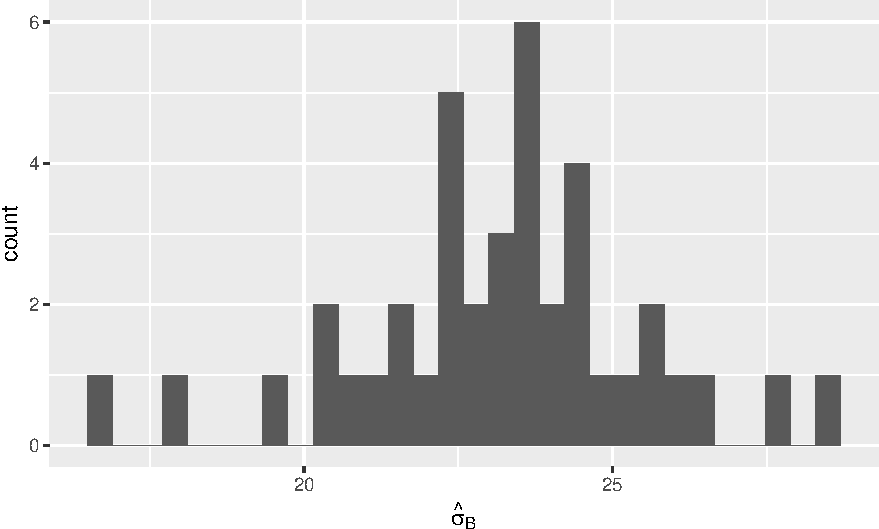
\includegraphics[width=0.7\linewidth]{statistical-computing_files/figure-latex/xbarsemc-1} 

}

\caption{Bootstrap replicates of sample mean done by mclapply}\label{fig:xbarsemc}
\end{figure}

Bootstrap standard error is given by

\begin{Shaded}
\begin{Highlighting}[]
\KeywordTok{sd}\NormalTok{(Xse)}
\CommentTok{#> [1] 2.59}
\end{Highlighting}
\end{Shaded}

Another way and possible also in Windows OS is \texttt{foreach::foreach}. Using \texttt{\%dopar\%} with pre-specifed workers instead of \texttt{\%do\%}, we can parallize the jobs. \texttt{.inorder} argument enable the task done in order different with the other functions. Default is \texttt{FALSE} and it is more stable.

When we do \texttt{foreach} parallization, we should distribute the jobs to workers manually.

\begin{Shaded}
\begin{Highlighting}[]
\NormalTok{cl <-}\StringTok{ }\NormalTok{parallel}\OperatorTok{::}\KeywordTok{makeCluster}\NormalTok{(MC_CORES)}
\NormalTok{doParallel}\OperatorTok{::}\KeywordTok{registerDoParallel}\NormalTok{(cl, }\DataTypeTok{cores =}\NormalTok{ MC_CORES)}
\NormalTok{parallel}\OperatorTok{::}\KeywordTok{clusterExport}\NormalTok{(cl, }\KeywordTok{c}\NormalTok{(}\StringTok{"X"}\NormalTok{, }\StringTok{"resample"}\NormalTok{))}
\NormalTok{parallel}\OperatorTok{::}\KeywordTok{clusterEvalQ}\NormalTok{(cl, }\KeywordTok{c}\NormalTok{(}\KeywordTok{library}\NormalTok{(dplyr), }\KeywordTok{library}\NormalTok{(data.table)))}
\CommentTok{#> [[1]]}
\CommentTok{#>  [1] "dplyr"      "stats"      "graphics"   "grDevices"  "utils"     }
\CommentTok{#>  [6] "datasets"   "methods"    "base"       "data.table" "dplyr"     }
\CommentTok{#> [11] "stats"      "graphics"   "grDevices"  "utils"      "datasets"  }
\CommentTok{#> [16] "methods"    "base"      }
\CommentTok{#> }
\CommentTok{#> [[2]]}
\CommentTok{#>  [1] "dplyr"      "stats"      "graphics"   "grDevices"  "utils"     }
\CommentTok{#>  [6] "datasets"   "methods"    "base"       "data.table" "dplyr"     }
\CommentTok{#> [11] "stats"      "graphics"   "grDevices"  "utils"      "datasets"  }
\CommentTok{#> [16] "methods"    "base"      }
\CommentTok{#> }
\CommentTok{#> [[3]]}
\CommentTok{#>  [1] "dplyr"      "stats"      "graphics"   "grDevices"  "utils"     }
\CommentTok{#>  [6] "datasets"   "methods"    "base"       "data.table" "dplyr"     }
\CommentTok{#> [11] "stats"      "graphics"   "grDevices"  "utils"      "datasets"  }
\CommentTok{#> [16] "methods"    "base"}
\end{Highlighting}
\end{Shaded}

\begin{Shaded}
\begin{Highlighting}[]
\NormalTok{Xse_foreach <-}\StringTok{ }
\StringTok{  }\KeywordTok{foreach}\NormalTok{(}\DataTypeTok{b =} \DecValTok{1}\OperatorTok{:}\NormalTok{B, }\DataTypeTok{.combine =}\NormalTok{ c, }\DataTypeTok{.inorder =} \OtherTok{FALSE}\NormalTok{) }\OperatorTok\StringTok{ }\NormalTok{\{}
    \KeywordTok{resample}\NormalTok{(}\DataTypeTok{data =}\NormalTok{ X, }\DataTypeTok{statistic =}\NormalTok{ mean)}
\NormalTok{  \}}
\end{Highlighting}
\end{Shaded}

To end this process, make sure \texttt{stopCluster()}.

\begin{Shaded}
\begin{Highlighting}[]
\NormalTok{parallel}\OperatorTok{::}\KeywordTok{stopCluster}\NormalTok{(cl)}
\end{Highlighting}
\end{Shaded}

\begin{Shaded}
\begin{Highlighting}[]
\KeywordTok{tibble}\NormalTok{(}\DataTypeTok{se =}\NormalTok{ Xse_foreach) }\OperatorTok\StringTok{ }
\StringTok{  }\KeywordTok{ggplot}\NormalTok{(}\KeywordTok{aes}\NormalTok{(}\DataTypeTok{x =}\NormalTok{ se)) }\OperatorTok{+}
\StringTok{  }\KeywordTok{geom_histogram}\NormalTok{(}\DataTypeTok{bins =} \DecValTok{30}\NormalTok{) }\OperatorTok{+}
\StringTok{  }\KeywordTok{xlab}\NormalTok{(}\KeywordTok{expression}\NormalTok{(}\KeywordTok{hat}\NormalTok{(sigma)[B]))}
\end{Highlighting}
\end{Shaded}

\begin{figure}[H]

{\centering 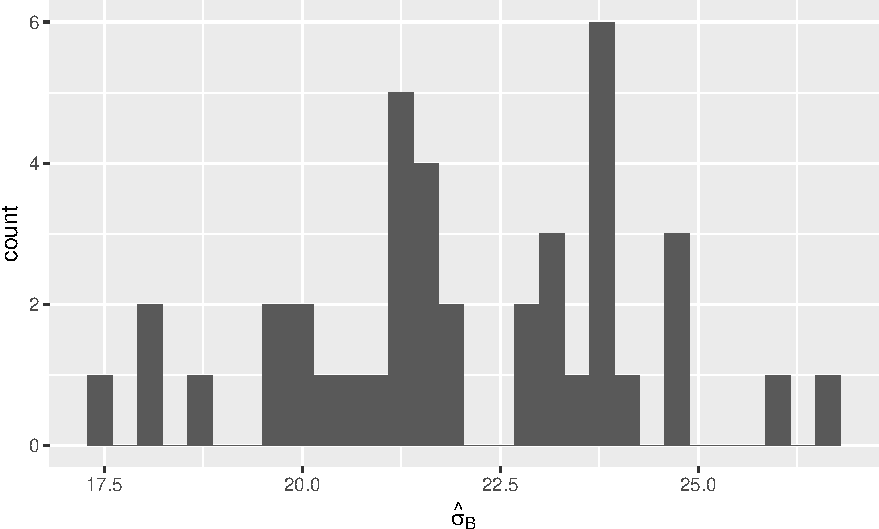
\includegraphics[width=0.7\linewidth]{statistical-computing_files/figure-latex/xbarsefor-1} 

}

\caption{Bootstrap replicates for sample mean done by foreach}\label{fig:xbarsefor}
\end{figure}

It gives boostrap standard error as

\begin{Shaded}
\begin{Highlighting}[]
\KeywordTok{sd}\NormalTok{(Xse_foreach)}
\CommentTok{#> [1] 1.88}
\end{Highlighting}
\end{Shaded}

Are these kinds of parallization useful?

\begin{Shaded}
\begin{Highlighting}[]
\NormalTok{microbenchmark}\OperatorTok{::}\KeywordTok{microbenchmark}\NormalTok{(}
  \StringTok{"MCLAPPLY2"}\NormalTok{ =}\StringTok{ }\NormalTok{\{}
\NormalTok{    parallel}\OperatorTok{::}\KeywordTok{mclapply}\NormalTok{(}
      \DecValTok{1}\OperatorTok{:}\NormalTok{B,}
      \ControlFlowTok{function}\NormalTok{(x) \{}\KeywordTok{resample}\NormalTok{(}\DataTypeTok{data =}\NormalTok{ X, }\DataTypeTok{statistic =}\NormalTok{ mean)\},}
      \DataTypeTok{mc.cores =} \DecValTok{2}
\NormalTok{    ) }\OperatorTok\StringTok{ }
\StringTok{      }\KeywordTok{unlist}\NormalTok{()}
\NormalTok{  \},}
  \StringTok{"MCLAPPLY3"}\NormalTok{ =}\StringTok{ }\NormalTok{\{}
\NormalTok{    parallel}\OperatorTok{::}\KeywordTok{mclapply}\NormalTok{(}
      \DecValTok{1}\OperatorTok{:}\NormalTok{B,}
      \ControlFlowTok{function}\NormalTok{(x) \{}\KeywordTok{resample}\NormalTok{(}\DataTypeTok{data =}\NormalTok{ X, }\DataTypeTok{statistic =}\NormalTok{ mean)\},}
      \DataTypeTok{mc.cores =} \DecValTok{3}
\NormalTok{    ) }\OperatorTok\StringTok{ }
\StringTok{      }\KeywordTok{unlist}\NormalTok{()}
\NormalTok{  \},}
  \StringTok{"MCLAPPLY4"}\NormalTok{ =}\StringTok{ }\NormalTok{\{}
\NormalTok{    parallel}\OperatorTok{::}\KeywordTok{mclapply}\NormalTok{(}
      \DecValTok{1}\OperatorTok{:}\NormalTok{B,}
      \ControlFlowTok{function}\NormalTok{(x) \{}\KeywordTok{resample}\NormalTok{(}\DataTypeTok{data =}\NormalTok{ X, }\DataTypeTok{statistic =}\NormalTok{ mean)\},}
      \DataTypeTok{mc.cores =} \DecValTok{4}
\NormalTok{    ) }\OperatorTok\StringTok{ }
\StringTok{      }\KeywordTok{unlist}\NormalTok{()}
\NormalTok{  \},}
  \StringTok{"FORLOOP"}\NormalTok{ =}\StringTok{ }\NormalTok{\{}
    \ControlFlowTok{for}\NormalTok{ (b }\ControlFlowTok{in} \DecValTok{1}\OperatorTok{:}\NormalTok{B) \{}
      \KeywordTok{resample}\NormalTok{(}\DataTypeTok{data =}\NormalTok{ X, }\DataTypeTok{statistic =}\NormalTok{ mean)}
\NormalTok{    \}}
\NormalTok{  \},}
  \DataTypeTok{times =} \DecValTok{5}\NormalTok{,}
  \DataTypeTok{unit =} \StringTok{"s"}
\NormalTok{) }\OperatorTok\StringTok{ }
\StringTok{  }\KeywordTok{autoplot}\NormalTok{()}
\end{Highlighting}
\end{Shaded}

\begin{figure}[H]

{\centering 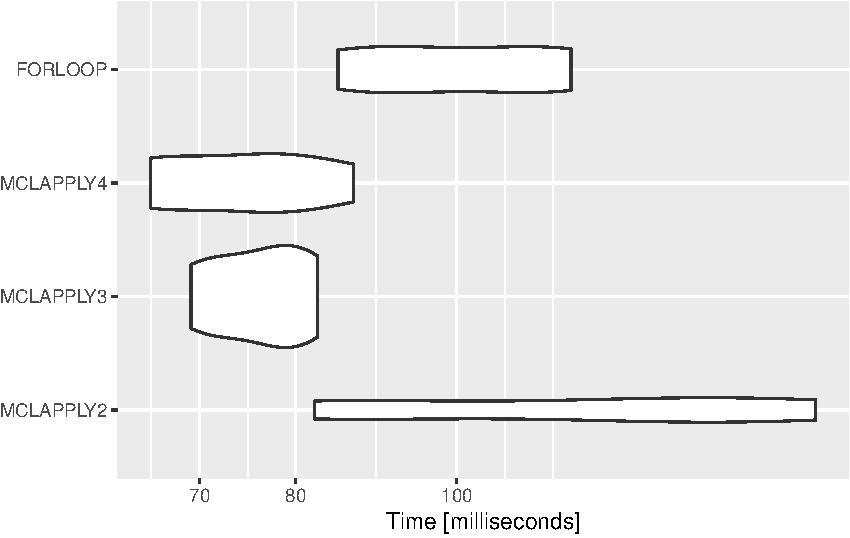
\includegraphics[width=0.7\linewidth]{statistical-computing_files/figure-latex/benchboot-1} 

}

\caption{Benchmark between mclapply and for loop}\label{fig:benchboot}
\end{figure}

Figure \ref{fig:benchboot} is comparing \texttt{for} loop with each \texttt{mc.cores}. It is clear that parallization is faster than ordinary loop. In fact, all these procedures can be done by \texttt{boot} package.

\begin{Shaded}
\begin{Highlighting}[]
\KeywordTok{library}\NormalTok{(boot)}
\end{Highlighting}
\end{Shaded}

Before performing bootstrap, we should define a \texttt{statistic} function. This function must take at least 2 arguments, data and index (\texttt{i}). About the second argument, \texttt{stype\ =\ c("i",\ "f",\ "w")} in \texttt{boot} is specifying in detail. Each \texttt{f} and \texttt{w} represents frequency and weight.

\begin{Shaded}
\begin{Highlighting}[]
\NormalTok{mean_boot <-}\StringTok{ }\ControlFlowTok{function}\NormalTok{(x, i) \{}
  \KeywordTok{mean}\NormalTok{(x[i])}
\NormalTok{\}}
\CommentTok{#-----------------------------}
\KeywordTok{boot}\NormalTok{(}\DataTypeTok{data =}\NormalTok{ X }\OperatorTok\StringTok{ }\KeywordTok{pull}\NormalTok{(), }\DataTypeTok{statistic =}\NormalTok{ mean_boot, }\DataTypeTok{R =}\NormalTok{ B)}
\CommentTok{#> }
\CommentTok{#> ORDINARY NONPARAMETRIC BOOTSTRAP}
\CommentTok{#> }
\CommentTok{#> }
\CommentTok{#> Call:}
\CommentTok{#> boot(data = X %>% pull(), statistic = mean_boot, R = B)}
\CommentTok{#> }
\CommentTok{#> }
\CommentTok{#> Bootstrap Statistics :}
\CommentTok{#>     original  bias    std. error}
\CommentTok{#> t1*     22.2  -0.117        2.14}
\end{Highlighting}
\end{Shaded}

It gives sample mean \texttt{original}, bootstrap bias \texttt{bias}, and bootstrap se \texttt{std.\ error}. We will cover bias later. Due to the programming fact, this is much more faster than the previous one. Also, we can parallize with this function. \texttt{parallel\ =\ c("no",\ "multicore",\ "snow")}. If we choose \texttt{"multicore"} option, we should specify \texttt{ncpus} as in \texttt{mclapply}. If \texttt{"snow"}, cluster should be supplied in \texttt{cl} argument like in \texttt{foreach}.

\begin{Shaded}
\begin{Highlighting}[]
\KeywordTok{boot}\NormalTok{(}
  \DataTypeTok{data =}\NormalTok{ X }\OperatorTok\StringTok{ }\KeywordTok{pull}\NormalTok{(),}
  \DataTypeTok{statistic =}\NormalTok{ mean_boot, }
  \DataTypeTok{R =}\NormalTok{ B,}
  \DataTypeTok{parallel =} \StringTok{"multicore"}\NormalTok{,}
  \DataTypeTok{ncpus =}\NormalTok{ MC_CORES}
\NormalTok{)}
\CommentTok{#> }
\CommentTok{#> ORDINARY NONPARAMETRIC BOOTSTRAP}
\CommentTok{#> }
\CommentTok{#> }
\CommentTok{#> Call:}
\CommentTok{#> boot(data = X %>% pull(), statistic = mean_boot, R = B, parallel = "multicore", }
\CommentTok{#>     ncpus = MC_CORES)}
\CommentTok{#> }
\CommentTok{#> }
\CommentTok{#> Bootstrap Statistics :}
\CommentTok{#>     original  bias    std. error}
\CommentTok{#> t1*     22.2   0.304        2.31}
\end{Highlighting}
\end{Shaded}

\begin{Shaded}
\begin{Highlighting}[]
\NormalTok{microbenchmark}\OperatorTok{::}\KeywordTok{microbenchmark}\NormalTok{(}
  \StringTok{"MCLAPPLY"}\NormalTok{ =}\StringTok{ }\NormalTok{\{}
\NormalTok{    parallel}\OperatorTok{::}\KeywordTok{mclapply}\NormalTok{(}
      \DecValTok{1}\OperatorTok{:}\NormalTok{B,}
      \ControlFlowTok{function}\NormalTok{(x) \{}\KeywordTok{resample}\NormalTok{(}\DataTypeTok{data =}\NormalTok{ X, }\DataTypeTok{statistic =}\NormalTok{ mean)\},}
      \DataTypeTok{mc.cores =}\NormalTok{ MC_CORES}
\NormalTok{    ) }\OperatorTok\StringTok{ }
\StringTok{      }\KeywordTok{unlist}\NormalTok{()}
\NormalTok{  \},}
  \StringTok{"BOOT"}\NormalTok{ =}\StringTok{ }\NormalTok{\{}
    \KeywordTok{boot}\NormalTok{(}
      \DataTypeTok{data =}\NormalTok{ X }\OperatorTok\StringTok{ }\KeywordTok{pull}\NormalTok{(),}
      \DataTypeTok{statistic =}\NormalTok{ mean_boot, }
      \DataTypeTok{R =}\NormalTok{ B,}
      \DataTypeTok{parallel =} \StringTok{"multicore"}\NormalTok{,}
      \DataTypeTok{ncpus =}\NormalTok{ MC_CORES}
\NormalTok{    )}
\NormalTok{  \},}
  \DataTypeTok{times =} \DecValTok{5}\NormalTok{,}
  \DataTypeTok{unit =} \StringTok{"s"}
\NormalTok{) }\OperatorTok\StringTok{ }
\StringTok{  }\KeywordTok{autoplot}\NormalTok{()}
\end{Highlighting}
\end{Shaded}

\begin{figure}[H]

{\centering 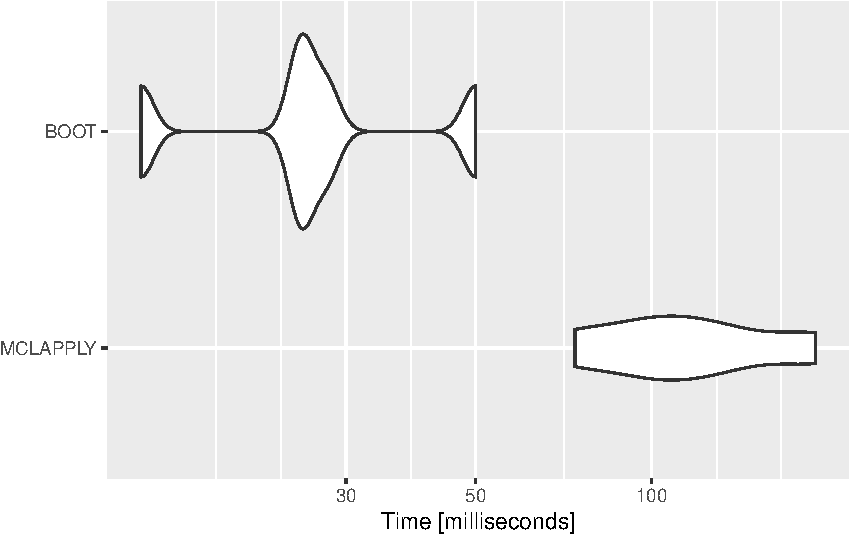
\includegraphics[width=0.7\linewidth]{statistical-computing_files/figure-latex/benchboot2-1} 

}

\caption{Benchmark between mclapply and boot}\label{fig:benchboot2}
\end{figure}

In Figure \ref{fig:benchboot2}, we can see the difference of the speed.

\hypertarget{estimation-of-correlation-coefficient}{%
\subsection{Estimation of correlation coefficient}\label{estimation-of-correlation-coefficient}}

Consider traditional bootstrap example \citep{Efron:1983bw}. The dataset is GPA scores of various entering classes at American law schools in 1973.

\begin{Shaded}
\begin{Highlighting}[]
\NormalTok{law }\OperatorTok\StringTok{ }
\StringTok{  }\KeywordTok{ggplot}\NormalTok{(}\KeywordTok{aes}\NormalTok{(}\DataTypeTok{x =}\NormalTok{ LSAT, }\DataTypeTok{y =}\NormalTok{ GPA)) }\OperatorTok{+}
\StringTok{  }\KeywordTok{geom_point}\NormalTok{()}
\end{Highlighting}
\end{Shaded}

\begin{figure}[H]

{\centering 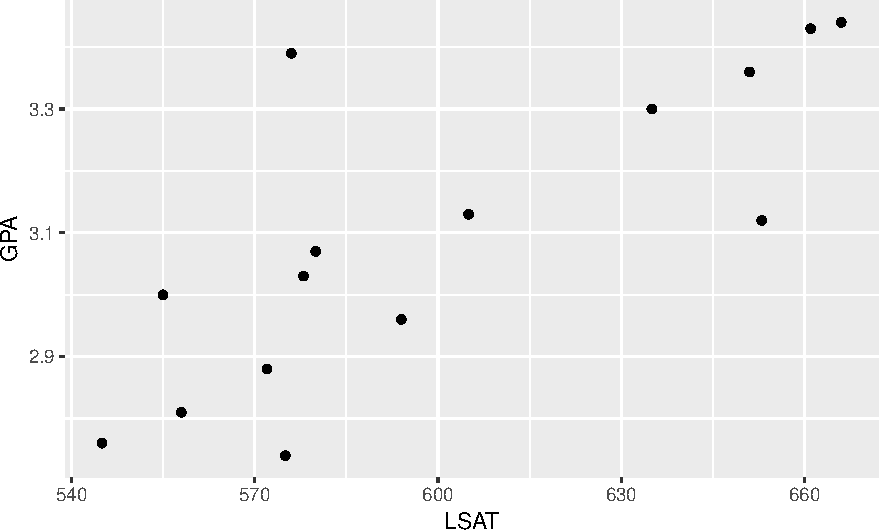
\includegraphics[width=0.7\linewidth]{statistical-computing_files/figure-latex/lawschool-1} 

}

\caption{The law school data (\cite{Efron:1983bw})}\label{fig:lawschool}
\end{figure}

Each point represents one law school.

\begin{itemize}
\tightlist
\item
  \texttt{LSAT}: average LSAT (national test) score of entering students
\item
  \texttt{GPA}: average GPA score of entering students
\end{itemize}

\BeginKnitrBlock{example}[Estimation of correlation coefficient]
\protect\hypertarget{exm:bootcor}{}{\label{exm:bootcor} \iffalse (Estimation of correlation coefficient) \fi{} }In this \((Y_i, Z_i) = (\text{LSAT}, \text{GPA})\) data set, we are interested in the correlation \(\rho\) of the two variables. Especially, we want to explore the distribution of \(\hat\rho\).
\EndKnitrBlock{example}

\begin{Shaded}
\begin{Highlighting}[]
\NormalTok{law }\OperatorTok\StringTok{ }
\StringTok{  }\KeywordTok{summarise}\NormalTok{(}\DataTypeTok{rho =} \KeywordTok{cor}\NormalTok{(LSAT, GPA))}
\CommentTok{#> # A tibble: 1 x 1}
\CommentTok{#>     rho}
\CommentTok{#>   <dbl>}
\CommentTok{#> 1 0.776}
\end{Highlighting}
\end{Shaded}

Let \(\mathbf{X}_i^T = (Y_i, Z_i)\) be each observation. Dependency should be kept, so we should sample \((Y_i, Z_i)\) pairs, not individuals.

\begin{algorithm}[H] \label{alg:algbootcor}
  \SetAlgoLined
  \SetKwInOut{Input}{input}
  \SetKwInOut{Output}{output}
  \Input{$n$ observations $\mathbf{X}_i^T = (Y_i, Z_i), \: i = 1, \ldots, n$}
  \For{$b \leftarrow 1$ \KwTo $B$}{
    Sampling with replacement $\mathbf{X}_{1}^{(b)}, \ldots, \mathbf{X}_n^{(b)}$ from the observed sample\;
    Sample correlation coefficient $$\hat\rho_b^{\ast} = \frac{\sum (Y_i^{(b)} - \overline{Y}^{(b)})(Z_i^{(b)} - \overline{Z}^{(b)})}{\sqrt{\sum (Y_i^{(b)} - \overline{Y}^{(b)})^2}\sqrt{\sum (Z_i^{(b)} - \overline{Z}^{(b)})^2}}$$\;
  }
  $\overline{\hat\rho^{\ast}} = \frac{1}{B} \sum\limits_{b = 1}^B \hat\rho_b^{\ast}$\;
  Bootsrap standard error $$\hat\sigma_B (\hat\rho) = \bigg[ \frac{1}{B - 1} \sum_{b = 1}^B (\hat\rho_b^{\ast} - \overline{\hat\rho^{\ast}})^2 \bigg]^{\frac{1}{2}}$$\; \label{alg:seout}
  \Output{$\hat\sigma_B (\hat\rho)$}
  \caption{Estimation of correlation coefficient - standard error}
\end{algorithm}

Following \citet{Efron:1983bw}, try \(B = 1000\).

\begin{Shaded}
\begin{Highlighting}[]
\NormalTok{boot_cor <-}\StringTok{ }\ControlFlowTok{function}\NormalTok{(x, i) \{}
  \KeywordTok{cor}\NormalTok{(x[i, }\DecValTok{1}\NormalTok{], x[i, }\DecValTok{2}\NormalTok{])}
\NormalTok{\}}
\CommentTok{#---------------------------}
\NormalTok{B <-}\StringTok{ }\DecValTok{1000}
\NormalTok{(rho <-}\StringTok{ }\KeywordTok{boot}\NormalTok{(law, }\DataTypeTok{statistic =}\NormalTok{ boot_cor, }\DataTypeTok{R =}\NormalTok{ B, }
            \DataTypeTok{parallel =} \StringTok{"multicore"}\NormalTok{, }\DataTypeTok{ncpus =}\NormalTok{ MC_CORES))}
\CommentTok{#> }
\CommentTok{#> ORDINARY NONPARAMETRIC BOOTSTRAP}
\CommentTok{#> }
\CommentTok{#> }
\CommentTok{#> Call:}
\CommentTok{#> boot(data = law, statistic = boot_cor, R = B, parallel = "multicore", }
\CommentTok{#>     ncpus = MC_CORES)}
\CommentTok{#> }
\CommentTok{#> }
\CommentTok{#> Bootstrap Statistics :}
\CommentTok{#>     original   bias    std. error}
\CommentTok{#> t1*    0.776 -0.00531       0.137}
\end{Highlighting}
\end{Shaded}

\BeginKnitrBlock{lemma}[Gaussian standard error of $\hat\rho$]
\protect\hypertarget{lem:cornorm}{}{\label{lem:cornorm} \iffalse (Gaussian standard error of \(\hat\rho\)) \fi{} }When the data follow Normal distribution, the standard error of \(\hat\rho\) can be estimated by

\[\hat\sigma_{NORM} = \frac{1 - \hat\rho^2}{\sqrt{n - 3}}\]
\EndKnitrBlock{lemma}

\begin{itemize}
\tightlist
\item
  \texttt{t0} is statistic computed from the sample, i.e.~correlation coefficient of the data
\item
  \texttt{t} is each bootstrap replicate, \texttt{matrix} object
\end{itemize}

Using \texttt{t}, we might draw empirical distribution and get standard error. In the real world, many data for scores follow normal. To check bootstrap works well, we compare the empirical distribution of \texttt{rho\$t} and one with Lemma \ref{lem:cornorm}.

\[\hat\sigma_{NORM} = \frac{1 - \hat\rho^2}{\sqrt{n - 3}} = 0.115\]

Construct \(\hat{F}\) by

\[\hat{F}_{NORM} \sim MVN\Big(\overline{\mathbf{x}}, \frac{n-1}{n}S \Big)\]

To see how normal population work, we \emph{draw bootstrap sample from the parametric maximum likeihood distribution}.

\[X_1^{\ast}, \ldots, X_n^{\ast} \sim \hat{F}_{NORM}\]

\texttt{boot} has arguments \texttt{sim}, \texttt{ran.gen} and \texttt{mle}.

\begin{itemize}
\tightlist
\item
  \texttt{sim}: type of simulation method. By default, \texttt{"ordinary"}. In this case, change this to \texttt{"parametric"}.
\item
  \texttt{ran.gen}: if \texttt{sim\ =\ "parametric"}, we should specify \texttt{ran.gen} generating random values. Function should have two arguments of \texttt{data} and \texttt{mle}.
\item
  \texttt{mle}: Second argument of \texttt{ran.gen}. MLE of parameters.
\end{itemize}

\begin{Shaded}
\begin{Highlighting}[]
\CommentTok{# mle --------------------------}
\NormalTok{lawmu <-}\StringTok{ }
\StringTok{  }\NormalTok{law }\OperatorTok\StringTok{ }
\StringTok{  }\KeywordTok{summarise_all}\NormalTok{(mean) }\OperatorTok\StringTok{ }
\StringTok{  }\KeywordTok{as.numeric}\NormalTok{()}
\NormalTok{lawcov <-}\StringTok{ }\KeywordTok{cov}\NormalTok{(law) }\OperatorTok{*}\StringTok{ }\KeywordTok{nrow}\NormalTok{(law) }\OperatorTok{/}\StringTok{ }\NormalTok{(}\KeywordTok{nrow}\NormalTok{(law) }\OperatorTok{-}\StringTok{ }\DecValTok{1}\NormalTok{)}
\CommentTok{# ran.gen ----------------------}
\NormalTok{gen_mvn <-}\StringTok{ }\ControlFlowTok{function}\NormalTok{(data, mle) \{}
\NormalTok{  mvtnorm}\OperatorTok{::}\KeywordTok{rmvnorm}\NormalTok{(}\KeywordTok{nrow}\NormalTok{(data), }\DataTypeTok{mean =}\NormalTok{ mle[[}\DecValTok{1}\NormalTok{]], }\DataTypeTok{sigma =}\NormalTok{ mle[[}\DecValTok{2}\NormalTok{]])}
\NormalTok{\}}
\CommentTok{# boot -------------------------}
\NormalTok{(rho_norm <-}\StringTok{ }
\StringTok{  }\KeywordTok{boot}\NormalTok{(}
\NormalTok{    law, }
    \DataTypeTok{statistic =}\NormalTok{ boot_cor, }
    \DataTypeTok{R =}\NormalTok{ B, }
    \DataTypeTok{sim =} \StringTok{"parametric"}\NormalTok{,}
    \DataTypeTok{ran.gen =}\NormalTok{ gen_mvn,}
    \DataTypeTok{mle =} \KeywordTok{list}\NormalTok{(lawmu, lawcov),}
    \DataTypeTok{parallel =} \StringTok{"multicore"}\NormalTok{, }
    \DataTypeTok{ncpus =}\NormalTok{ MC_CORES}
\NormalTok{  ))}
\CommentTok{#> }
\CommentTok{#> PARAMETRIC BOOTSTRAP}
\CommentTok{#> }
\CommentTok{#> }
\CommentTok{#> Call:}
\CommentTok{#> boot(data = law, statistic = boot_cor, R = B, sim = "parametric", }
\CommentTok{#>     ran.gen = gen_mvn, mle = list(lawmu, lawcov), parallel = "multicore", }
\CommentTok{#>     ncpus = MC_CORES)}
\CommentTok{#> }
\CommentTok{#> }
\CommentTok{#> Bootstrap Statistics :}
\CommentTok{#>     original  bias    std. error}
\CommentTok{#> t1*    0.776 -0.0126       0.121}
\end{Highlighting}
\end{Shaded}

As \(B \rightarrow \infty\), \(\hat\sigma_B\) approximates \(\hat\sigma_{NORM} = 0.115\). See the similarity of the two values.

\begin{Shaded}
\begin{Highlighting}[]
\KeywordTok{tibble}\NormalTok{(}
  \DataTypeTok{rho1 =}\NormalTok{ rho}\OperatorTok{$}\NormalTok{t[,}\DecValTok{1}\NormalTok{],}
  \DataTypeTok{rho2 =}\NormalTok{ rho_norm}\OperatorTok{$}\NormalTok{t[,}\DecValTok{1}\NormalTok{]}
\NormalTok{) }\OperatorTok\StringTok{ }
\StringTok{  }\KeywordTok{ggplot}\NormalTok{() }\OperatorTok{+}
\StringTok{  }\KeywordTok{geom_histogram}\NormalTok{(}\DataTypeTok{bins =} \DecValTok{30}\NormalTok{, }\KeywordTok{aes}\NormalTok{(}\DataTypeTok{x =}\NormalTok{ rho1, }\DataTypeTok{y =}\NormalTok{ ..density..)) }\OperatorTok{+}
\StringTok{  }\KeywordTok{stat_density}\NormalTok{(}\KeywordTok{aes}\NormalTok{(}\DataTypeTok{x =}\NormalTok{ rho2, }\DataTypeTok{y =}\NormalTok{ ..density..), }\DataTypeTok{geom =} \StringTok{"line"}\NormalTok{, }\DataTypeTok{col =} \KeywordTok{gg_hcl}\NormalTok{(}\DecValTok{1}\NormalTok{)) }\OperatorTok{+}
\StringTok{  }\KeywordTok{xlab}\NormalTok{(}\KeywordTok{expression}\NormalTok{(}\KeywordTok{hat}\NormalTok{(rho)}\OperatorTok{^}\StringTok{"*"}\NormalTok{))}
\end{Highlighting}
\end{Shaded}

\begin{figure}[H]

{\centering 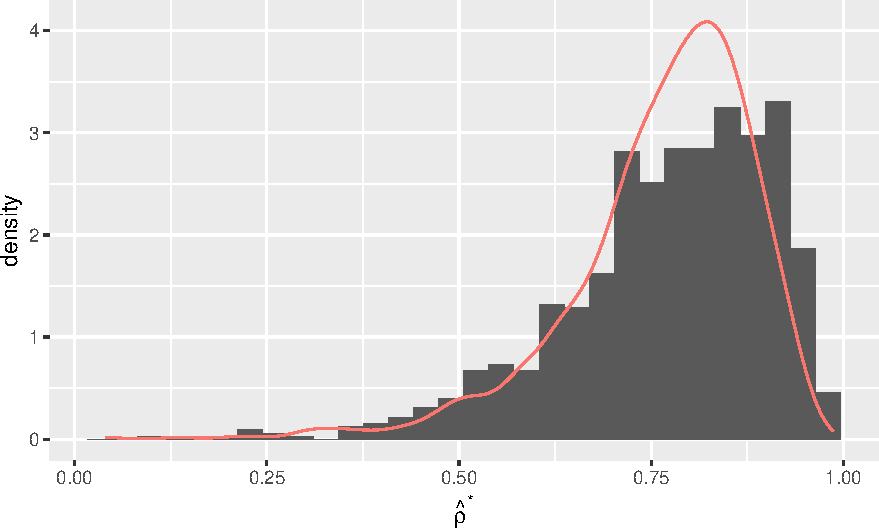
\includegraphics[width=0.7\linewidth]{statistical-computing_files/figure-latex/bootrep-1} 

}

\caption{Bootstrap replicates for correlation in law school data - histogram of ordinary, line of parametric}\label{fig:bootrep}
\end{figure}

See Figure \ref{fig:bootrep}. Normal density has a similar shape to ordinary bootstrap, except that normal bootstrap falls off more quickly at the right tail.

\hypertarget{boostrap-bias}{%
\subsection{Boostrap bias}\label{boostrap-bias}}

\BeginKnitrBlock{definition}[Bias]
\protect\hypertarget{def:biasdef}{}{\label{def:biasdef} \iffalse (Bias) \fi{} }Bias of a estimator \(\theta\) is

\[\beta := E(\hat\theta) - \theta\]
\EndKnitrBlock{definition}

Note that \(\beta\) is a kind of function of the unkown probability ditribution \(F\).

\[\beta = \beta(F)\]

In this sense, bootstrap estimate of \(\beta\) can be given as

\begin{equation}
  \hat\beta_B = \beta(\hat{F}) = E_{F^{\ast}} \Big[ \theta(\hat{F}^{\ast}) - \theta(\hat{F}) \Big]
  \label{eq:bootbias}
\end{equation}

Here, expectation \(E_{F^{\ast}}\) can be approximated by Monte Carlo methods. Sampling

\[X_1^{\ast}, \ldots, X_n^{\ast} \stackrel{iid}{\sim}F^{\ast}\]

compute

\begin{equation}
  \hat\beta_B \approx \overline{\hat\theta^{\ast}} - \hat\theta = \frac{1}{B} \sum_{b = 1}^B ( \hat\theta_b^{\ast} - \hat\theta)
  \label{eq:bootbiasest}
\end{equation}

In Algorithm \(\ref{alg:algbootcor}\), we only need to replace Step \(\ref{alg:seout}\) with above Equation \eqref{eq:bootbiasest}.

\BeginKnitrBlock{theorem}[Bootstrap Bias]
\protect\hypertarget{thm:bootbet}{}{\label{thm:bootbet} \iffalse (Bootstrap Bias) \fi{} }Bootstrap estimate of bias for any estimator \(\hat\theta(X_1, \ldots, X_n)\) of \(\theta\) is

\[\hat\beta_B = \overline{\hat\theta^{\ast}} - \hat\theta\]

where \(\overline{\hat\theta^{\ast}} = \frac{1}{B} \sum\limits_{b = 1}^B \hat\theta_b^{\ast}\) and \(\hat\theta = \hat\theta(X_1, \ldots, X_n)\), i.e.~one estimated by observed sample
\EndKnitrBlock{theorem}

Is it reasonable to compare \(\overline{\hat\theta^{\ast}}\) with \(\hat\theta\) even though we do not know the true one? This is natural from bootstrap construction. Bootstrap takes its population as observed sample of which distribution is \(\hat{F}\). So \(\hat\theta\) of pseudo-population, \(\theta(\hat{F})\) of Equation \eqref{eq:bootbias}, is able to represent the true value.

\begin{algorithm}[H] \label{alg:algbootcor2}
  \SetAlgoLined
  \SetKwInOut{Input}{input}
  \SetKwInOut{Output}{output}
  \Input{$n$ observations $\mathbf{X}_i^T = (Y_i, Z_i), \: i = 1, \ldots, n$}
  \For{$b \leftarrow 1$ \KwTo $B$}{
    Sampling with replacement $\mathbf{X}_{1}^{(b)}, \ldots, \mathbf{X}_n^{(b)}$ from the observed sample\;
    Sample correlation coefficient $$\hat\rho_b^{\ast} = \frac{\sum (Y_i^{(b)} - \overline{Y}^{(b)})(Z_i^{(b)} - \overline{Z}^{(b)})}{\sqrt{\sum (Y_i^{(b)} - \overline{Y}^{(b)})^2}\sqrt{\sum (Z_i^{(b)} - \overline{Z}^{(b)})^2}}$$\;
  }
  $\overline{\hat\rho^{\ast}} = \frac{1}{B} \sum\limits_{b = 1}^B \hat\rho_b^{\ast}$\;
  Bootsrap bias $$\hat\beta_B = \overline{\hat\rho^{\ast}} - \hat\rho$$\; \label{alg:biasout}
  \Output{$\hat\beta_B$}
  \caption{Estimation of correlation coefficient - bias}
\end{algorithm}

If

\[\frac{\hat\beta_B}{\hat\sigma_B} < \frac{1}{4}\]

then it might be okay to ignore the bias, i.e.~not necessary to adjust for it\citep{Efron:1994aa}.

Refer to Example \ref{exm:bootcor}. \texttt{boot::boot()} have given following output.

\begin{Shaded}
\begin{Highlighting}[]
\NormalTok{rho}
\CommentTok{#> }
\CommentTok{#> ORDINARY NONPARAMETRIC BOOTSTRAP}
\CommentTok{#> }
\CommentTok{#> }
\CommentTok{#> Call:}
\CommentTok{#> boot(data = law, statistic = boot_cor, R = B, parallel = "multicore", }
\CommentTok{#>     ncpus = MC_CORES)}
\CommentTok{#> }
\CommentTok{#> }
\CommentTok{#> Bootstrap Statistics :}
\CommentTok{#>     original   bias    std. error}
\CommentTok{#> t1*    0.776 -0.00531       0.137}
\end{Highlighting}
\end{Shaded}

\(\hat\beta_B\) is \texttt{bias}.

\BeginKnitrBlock{example}[Bootstrap estimate of a ratio estimate]
\protect\hypertarget{exm:ratbias}{}{\label{exm:ratbias} \iffalse (Bootstrap estimate of a ratio estimate) \fi{} }Consider medical patch data from \citet{Efron:1994aa}. It contains measurement for hormone into the blood stream of 8 subjects after wearing a medical patch. There are three different patches.

\begin{itemize}
  \item placebo patch
  \item old patch, manufactured at an older plant
  \item new patch, manufactured at a new plant
\end{itemize}

Define a parameter \text{bioequivalence} by

\[\theta = \frac{E(new) - E(old)}{E(old) - E(placebo)} \le 0.2\]

This is the parameter of our interest.
\EndKnitrBlock{example}

\begin{Shaded}
\begin{Highlighting}[]
\KeywordTok{as_tibble}\NormalTok{(bootstrap}\OperatorTok{::}\NormalTok{patch)}
\CommentTok{#> # A tibble: 8 x 6}
\CommentTok{#>   subject placebo oldpatch newpatch     z     y}
\CommentTok{#>     <int>   <dbl>    <dbl>    <dbl> <dbl> <dbl>}
\CommentTok{#> 1       1    9243    17649    16449  8406 -1200}
\CommentTok{#> 2       2    9671    12013    14614  2342  2601}
\CommentTok{#> 3       3   11792    19979    17274  8187 -2705}
\CommentTok{#> 4       4   13357    21816    23798  8459  1982}
\CommentTok{#> 5       5    9055    13850    12560  4795 -1290}
\CommentTok{#> 6       6    6290     9806    10157  3516   351}
\CommentTok{#> 7       7   12412    17208    16570  4796  -638}
\CommentTok{#> 8       8   18806    29044    26325 10238 -2719}
\end{Highlighting}
\end{Shaded}

In \texttt{patch},

\begin{itemize}
\tightlist
\item
  \texttt{z}: \texttt{oldpatch} - \texttt{placebo}
\item
  \texttt{y}: \texttt{newpatch} - \texttt{oldpatch}
\end{itemize}

We only need these two columns. \texttt{z} goes to denominator, \texttt{y} to numerator.

\begin{Shaded}
\begin{Highlighting}[]
\NormalTok{bioequiv <-}\StringTok{ }\ControlFlowTok{function}\NormalTok{(x, i) \{}
  \CommentTok{# select(z, y)}
  \KeywordTok{mean}\NormalTok{(x[i, }\DecValTok{2}\NormalTok{]) }\OperatorTok{/}\StringTok{ }\KeywordTok{mean}\NormalTok{(x[i, }\DecValTok{1}\NormalTok{])}
\NormalTok{\}}
\CommentTok{#---------------------------}
\NormalTok{B <-}\StringTok{ }\DecValTok{2000}
\NormalTok{(ratio <-}\StringTok{ }
\StringTok{  }\NormalTok{bootstrap}\OperatorTok{::}\NormalTok{patch }\OperatorTok\StringTok{ }
\StringTok{  }\KeywordTok{select}\NormalTok{(z, y) }\OperatorTok\StringTok{ }
\StringTok{  }\KeywordTok{boot}\NormalTok{(}
    \DataTypeTok{statistic =}\NormalTok{ bioequiv,}
    \DataTypeTok{R =}\NormalTok{ B,}
    \DataTypeTok{parallel =} \StringTok{"multicore"}\NormalTok{,}
    \DataTypeTok{ncpus =}\NormalTok{ MC_CORES}
\NormalTok{  ))}
\CommentTok{#> }
\CommentTok{#> ORDINARY NONPARAMETRIC BOOTSTRAP}
\CommentTok{#> }
\CommentTok{#> }
\CommentTok{#> Call:}
\CommentTok{#> boot(data = ., statistic = bioequiv, R = B, parallel = "multicore", }
\CommentTok{#>     ncpus = MC_CORES)}
\CommentTok{#> }
\CommentTok{#> }
\CommentTok{#> Bootstrap Statistics :}
\CommentTok{#>     original  bias    std. error}
\CommentTok{#> t1*  -0.0713 0.00708      0.0994}
\end{Highlighting}
\end{Shaded}

\texttt{broom::tidy()} gives tidies a \texttt{boot} object so that we can deal with above three statistic more easily.

\begin{Shaded}
\begin{Highlighting}[]
\NormalTok{(ratio_tidy <-}\StringTok{ }
\StringTok{  }\NormalTok{broom}\OperatorTok{::}\KeywordTok{tidy}\NormalTok{(ratio) }\OperatorTok\StringTok{ }
\StringTok{    }\KeywordTok{mutate}\NormalTok{(}
      \DataTypeTok{bias_se =}\NormalTok{ bias }\OperatorTok{/}\StringTok{ }\NormalTok{std.error,}
      \DataTypeTok{ignore_bias =} \KeywordTok{ifelse}\NormalTok{(bias_se }\OperatorTok{<}\StringTok{ }\FloatTok{.25}\NormalTok{, }\StringTok{"ignore bias"}\NormalTok{, }\StringTok{"adjust for bias"}\NormalTok{)}
\NormalTok{    ))}
\CommentTok{#> # A tibble: 1 x 5}
\CommentTok{#>   statistic    bias std.error bias_se ignore_bias}
\CommentTok{#>       <dbl>   <dbl>     <dbl>   <dbl> <chr>      }
\CommentTok{#> 1   -0.0713 0.00708    0.0994  0.0712 ignore bias}
\end{Highlighting}
\end{Shaded}

Since \(\frac{\hat\beta_B}{\hat\sigma_B} = 0.071\), we \(\text{ignore bias}\).

\hypertarget{jackknife}{%
\section{Jackknife}\label{jackknife}}

Jackknife is another resampling method, which was developed earlier than bootstrap. Instead of bootstrap sample \(\mathbf{X}^{(b)}\), \emph{jackknife sample} \(\mathbf{X}_{(i)}\) will be used. It leaves out the \(i\)-th observation.

\begin{equation}
  \mathbf{X}^{(i)} = (X_1^{(i)}, \ldots, X_{i - 1}^{(i)}, X_{i + 1}^{(i)}, \ldots, X_n^{(i)})^T
  \label{eq:jacksam}
\end{equation}

For each \(\mathbf{X}^{(i)}\), \emph{jackknife replicate} which is a form of our interest is computed.

\begin{equation}
  \hat\theta^{(i)} = \hat\theta(\mathbf{X}^{(i)})
  \label{eq:jackrep}
\end{equation}

so that we can get its empirical distribution.

\begin{figure}[H]

{\centering 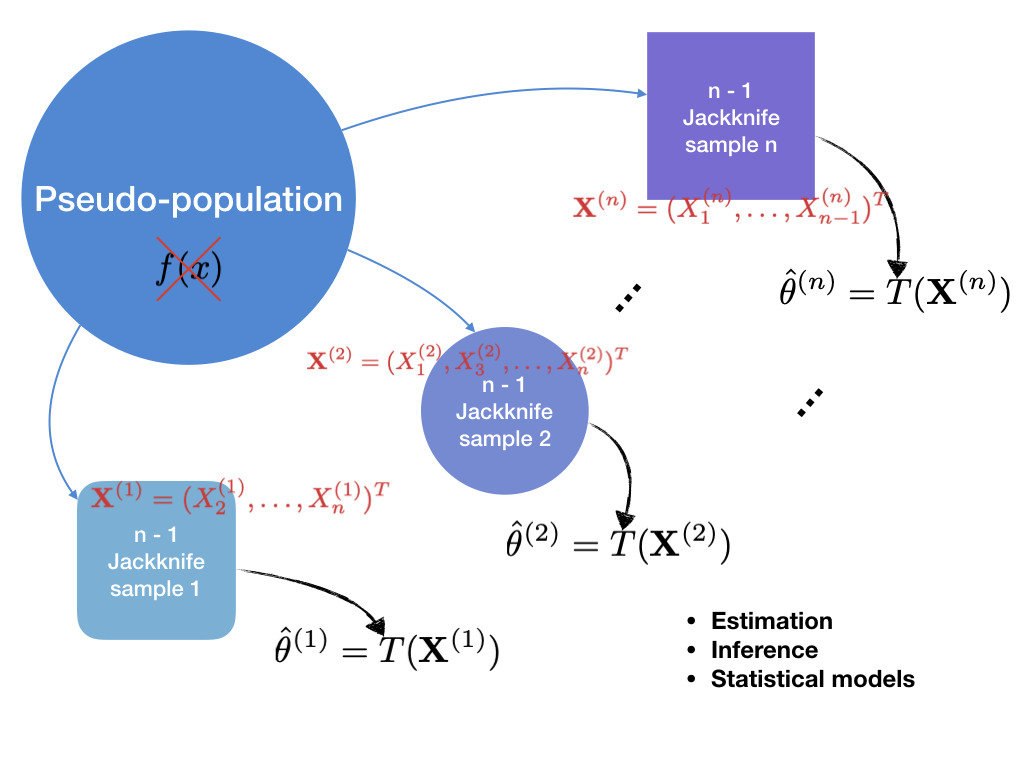
\includegraphics[width=0.7\linewidth]{images/jack} 

}

\caption{Leave-one-out sampling}\label{fig:jackfig}
\end{figure}

\hypertarget{jackknife-standard-error}{%
\subsection{Jackknife standard error}\label{jackknife-standard-error}}

As in Section \ref{bootapprox}, we start with simple example, estimating sample mean. Refer to Example \ref{exm:bootave}. We have seen estimated standard error \(\hat\sigma\) and boostrap estimate of standard error \(\hat\sigma_B\) in Theorems \ref{thm:samplemean} and \ref{thm:bootse}.

\BeginKnitrBlock{theorem}[Jackknife standard error for sample mean]
\protect\hypertarget{thm:jacksebar}{}{\label{thm:jacksebar} \iffalse (Jackknife standard error for sample mean) \fi{} }Let

\[\overline{X}_{(i)} := \frac{n \overline{X} - X_i}{n - 1} = \frac{1}{n - 1}\sum_{j \neq i} X_j\]

be the sample average of the set deleting \(i\)-th point. Write average of the deleted averages by \(\overline{X}_{(.)} = \frac{1}{n} \sum\limits_{i = 1}^n \overline{X}_{(i)}\). By construction,

\[\overline{X}_{(.)} = \overline{X}\]

Jackknife estimate of standard error for sample mean \(\overline{X}\) is

\[\hat\sigma_J = \bigg[ \frac{n - 1}{n} \sum_{i = 1}^n \Big(\overline{X}_{(i)} - \overline{X}_{(.)} \Big)^2 \bigg]^{\frac{1}{2}}\]
\EndKnitrBlock{theorem}

\BeginKnitrBlock{remark}
\iffalse{} {Remark. } \fi{}\[\hat\sigma = \hat\sigma_J\]
\EndKnitrBlock{remark}

\BeginKnitrBlock{proof}
\iffalse{} {Proof. } \fi{}Note that

\[\overline{X}_{(i)} = \frac{n \overline{X} - X_i}{n - 1}\]

By construction,

\begin{equation*}
  \begin{split}
    \overline{X}_{(.)} & = \frac{1}{n} \sum_{i = 1}^n \bigg[ \frac{n \overline{X} - X_i}{n - 1} \bigg] \\
    & = \frac{n \overline{X}}{n - 1} - \frac{\overline{X}}{n - 1} \\
    & = \overline{X}
  \end{split}
\end{equation*}

It follows that

\begin{equation*}
  \begin{split}
    \hat\sigma_J^2 = \frac{n - 1}{n} \sum_{i = 1}^n \Big(\overline{X}_{(i)} - \overline{X}_{(.)} \Big)^2 & = \frac{n - 1}{n} \sum_{i = 1}^n \bigg( \frac{n \overline{X} - X_i}{n - 1} - \overline{X} \bigg)^2 \\
    & = \frac{n - 1}{n} \sum_{i = 1}^n \bigg( \frac{\overline{X} - X_i}{n - 1} \bigg)^2 \\
    & = \frac{1}{n (n - 1)} \sum_{i = 1}^n \Big( X_i - \overline{X} \Big)^2 \\
    & = \hat\sigma^2
  \end{split}
\end{equation*}
\EndKnitrBlock{proof}

Using a set of jackknife replicates, get empirical distribution of this estimator such as standard error and bias.

\begin{algorithm}[H] \label{alg:algjack}
  \SetAlgoLined
  \SetKwInOut{Input}{input}
  \SetKwInOut{Output}{output}
  \KwData{$n$ observations $x_1, \ldots, x_n$}
  \Input{statistic of interest $\hat\theta$}
  \For{$i \leftarrow 1$ \KwTo $n$}{
    Subset of $\mathbf{X}$ that leaves out the $i$-th observation $X_1, \ldots, X_{i - 1}, X_{i + 1}, \ldots, X_n$\;
    Compute estimate $$\hat\theta(X_1, \ldots, X_{i - 1}, X_{i + 1}, \ldots, X_n) \equiv \hat\theta_{(i)}$$\;
  }
  $\hat\theta_{(.)} = \frac{1}{n} \sum\limits_{i = 1}^n \hat\theta_{(i)}$\;
  Jackknife standard error $$\hat\sigma_J = \bigg[ \frac{n - 1}{n} \sum_{i = 1}^n (\hat\theta_{(i)} - \hat\theta_{(.)})^2 \bigg]^{\frac{1}{2}}$$\;
  \Output{$\hat\sigma_J$}
  \caption{Jackknife algorithm}
\end{algorithm}

Now extend to any statistic such as correlation \ref{exm:bootcor}. Let \(\hat\theta \equiv \hat\theta(X_1, \ldots, X_n)\) be the statistic of interest. Suppose that

\[X_1, \ldots, X_n \stackrel{iid}{\sim}F\]

Let \(\mathbf{P}\) be a probability mass vector for each \(X_i\) and let \(\mathbf{P}^{\ast}\) be a vector for bootstrap sample. Recall that each point has a mass of

\[\frac{1}{n}\]

Then we have

\[\mathbf{P}^{\ast} \sim Multi(n, \mathbf{P}_0)\]

with \(\mathbf{P}_0 = \frac{1}{n}\mathbf{1} \in \mathbb{R}^n\). We already have seend that the bootstrap standard error is

\[\hat\sigma_B = \Big[ Var \hat\theta(\mathbf{P}^{\ast}) \Big]^{\frac{1}{2}}\]

In comparison, the jackknife resamples leaving out one observation so that

\[\mathbf{P}_{(i)} = \frac{1}{n - 1} (1, \ldots, 1, \overset{i\text{-th}}{0}, 1, \ldots, 1)^T, \quad i = 1, \ldots, n\]

\citet{Efron:1983bw} draws a picture that indicates this difference between resampling procedure of bootstrap and jackknife. Among \(\{ X_1, X_2, X_3 \}\), bootstrap sample with replacement with probability \(\frac{1}{3}\). Jackknife leaves out one in each sample.

\begin{figure}[H]

{\centering \includegraphics[width=0.7\linewidth]{images/efron} 

}

\caption{Bootstrap and Jackknife sampling points - $\cdot$ is bootstrap and $\circ$ is jackknife}\label{fig:efronfig}
\end{figure}

\BeginKnitrBlock{lemma}
\protect\hypertarget{lem:jackboot}{}{\label{lem:jackboot} }Jackknife estimation approximates \(\hat\theta(\mathbf{P})\) by a linear function of \(\mathbf{P}\), say \(\hat\theta_L(\mathbf{P})\).

\[\hat\theta_L(\mathbf{P}) = \hat\theta_{(.)} + (\mathbf{P} - \mathbf{P}^0)^T U\]

where \(\hat\theta_{(.)} = \frac{1}{n} \sum_i \hat\theta_{(i)} = \frac{1}{n} \sum_i \hat\theta(\mathbf{P}_{(i)})\), \(U_i = (n - 1)(\hat\theta_{(.)} - \hat\theta_{(.)})\), and \(U = \begin{bmatrix} U_1 & \cdots & U_n \end{bmatrix}\).
\EndKnitrBlock{lemma}

\BeginKnitrBlock{theorem}[Jackknife standard error]
\protect\hypertarget{thm:jackse}{}{\label{thm:jackse} \iffalse (Jackknife standard error) \fi{} }Let \(\hat\theta_L\) of Lemma \ref{lem:jackboot} be the statistic of interest. Then the Jackknife estimate of standard error for \(\hat\theta_L\) is

\[\hat\sigma_J = \bigg[ \frac{n}{n - 1} Var \hat\theta_L(\mathbf{P}^{\ast}) \bigg]^{\frac{1}{2}}\]

where \(\hat\theta_L(\mathbf{P}^{\ast})\) is the bootstrap estimate.
\EndKnitrBlock{theorem}

\begin{Shaded}
\begin{Highlighting}[]
\NormalTok{cor_jack <-}\StringTok{ }\ControlFlowTok{function}\NormalTok{(x) \{}
  \KeywordTok{cor}\NormalTok{(x[,}\DecValTok{1}\NormalTok{], x[,}\DecValTok{2}\NormalTok{])}
\NormalTok{\}}
\CommentTok{#----------------------}
\NormalTok{jack_cor <-}\StringTok{ }\ControlFlowTok{function}\NormalTok{(x, data) \{}
  \CommentTok{# sampling with replacement}
\NormalTok{  xb <-}
\StringTok{    }\NormalTok{data }\OperatorTok\StringTok{ }
\StringTok{    }\KeywordTok{data.table}\NormalTok{() }\OperatorTok\StringTok{ }
\StringTok{    }\NormalTok{.[}\OperatorTok{-}\NormalTok{x]}
  \CommentTok{# estimator}
  \KeywordTok{cor}\NormalTok{(xb[,}\DecValTok{1}\NormalTok{], xb[,}\DecValTok{2}\NormalTok{]) }\OperatorTok\StringTok{ }\KeywordTok{as.numeric}\NormalTok{()}
\NormalTok{\}}
\CommentTok{#---------------------}
\NormalTok{law_jack <-}\StringTok{ }
\StringTok{  }\NormalTok{parallel}\OperatorTok{::}\KeywordTok{mclapply}\NormalTok{(}
    \DecValTok{1}\OperatorTok{:}\KeywordTok{nrow}\NormalTok{(law), }
\NormalTok{    jack_cor, }
    \DataTypeTok{data =}\NormalTok{ law,}
    \DataTypeTok{mc.cores =}\NormalTok{ MC_CORES}
\NormalTok{  ) }\OperatorTok\StringTok{ }
\StringTok{  }\KeywordTok{unlist}\NormalTok{()}
\CommentTok{#--------------------}
\KeywordTok{sqrt}\NormalTok{((}\KeywordTok{nrow}\NormalTok{(law) }\OperatorTok{-}\StringTok{ }\DecValTok{1}\NormalTok{) }\OperatorTok{*}\StringTok{ }\KeywordTok{mean}\NormalTok{((law_jack }\OperatorTok{-}\StringTok{ }\KeywordTok{mean}\NormalTok{(law_jack))}\OperatorTok{^}\DecValTok{2}\NormalTok{))}
\CommentTok{#> [1] 0.143}
\end{Highlighting}
\end{Shaded}

\begin{figure}[H]

{\centering \includegraphics[width=0.7\linewidth]{statistical-computing_files/figure-latex/jackcor-1} 

}

\caption{Jackknife estimate of correlation}\label{fig:jackcor}
\end{figure}

Visually, the distribution is quite similar to of bootstrap \ref{fig:bootrep}. Also, standard error is not that different.

\texttt{bootstrap} library provides \texttt{jackknife()} function. Since this kind of \emph{leave-one-out} procedure does not have randomness, the result is exactly same.

\begin{Shaded}
\begin{Highlighting}[]
\NormalTok{cor_law <-}\StringTok{ }\ControlFlowTok{function}\NormalTok{(x, xdata) \{}
  \KeywordTok{cor}\NormalTok{(xdata[x, }\DecValTok{1}\NormalTok{], xdata[x, }\DecValTok{2}\NormalTok{])}
\NormalTok{\}}
\CommentTok{#------------------------------}
\NormalTok{bootstrap}\OperatorTok{::}\KeywordTok{jackknife}\NormalTok{(}\DecValTok{1}\OperatorTok{:}\KeywordTok{nrow}\NormalTok{(law), cor_law, }\DataTypeTok{xdata =}\NormalTok{ law)}
\CommentTok{#> $jack.se}
\CommentTok{#> [1] 0.143}
\CommentTok{#> }
\CommentTok{#> $jack.bias}
\CommentTok{#>           GPA}
\CommentTok{#> LSAT -0.00647}
\CommentTok{#> }
\CommentTok{#> $jack.values}
\CommentTok{#>  [1] 0.893 0.764 0.755 0.776 0.731 0.780 0.785 0.736 0.752 0.776 0.818}
\CommentTok{#> [12] 0.786 0.740 0.767 0.780}
\CommentTok{#> }
\CommentTok{#> $call}
\CommentTok{#> bootstrap::jackknife(x = 1:nrow(law), theta = cor_law, xdata = law)}
\end{Highlighting}
\end{Shaded}

\hypertarget{jackknife-bias}{%
\subsection{Jackknife bias}\label{jackknife-bias}}

Consider bias \(\beta\) of \(\hat\theta = \hat\theta(\hat{F})\) \ref{def:biasdef}.

\BeginKnitrBlock{lemma}[Quenouille's estimate for bias]
\protect\hypertarget{lem:biasest}{}{\label{lem:biasest} \iffalse (Quenouille's estimate for bias) \fi{} }In the notation of Lemma \ref{lem:jackboot}, Quenouille's estimate for bias is

\[\hat\beta_J = (n - 1) (\hat\theta_{(.)} - \hat\theta)\]
\EndKnitrBlock{lemma}

As in the previous section, there is a relationship between a bias estimate \ref{lem:biasest} and Bootstrap bias \ref{thm:bootbet}.

\BeginKnitrBlock{lemma}
\protect\hypertarget{lem:bootquad}{}{\label{lem:bootquad} }Jackknife estimation approximates \(\hat\theta(\mathbf{P})\) by a quadratic function of \(\mathbf{P}\), say \(\hat\theta_Q(\mathbf{P})\).

\[\hat\theta_Q (\mathbf{P}_0) = a + (\mathbf{P} - \mathbf{P}_0)^T \mathbf{b} + \frac{1}{2} (\mathbf{P} - \mathbf{P}_0)^T \mathbf{c} (\mathbf{P} - \mathbf{P}_0)\]
\EndKnitrBlock{lemma}

From this Lemma, Jackknife bias \(\hat\beta_J\) can be derived as follows.

\BeginKnitrBlock{theorem}[Jackknife bias]
\protect\hypertarget{thm:jackbet}{}{\label{thm:jackbet} \iffalse (Jackknife bias) \fi{} }Let \(\hat\theta_Q (\mathbf{P})\) be any quadratic satisfying

\[\hat\theta_Q (\mathbf{P}_0) = \hat\theta (\mathbf{P}_0) = \hat\theta \quad \text{and} \quad \hat\theta_Q (\mathbf{P}_{(i)}) = \hat\theta (\mathbf{P}_{(i)})\]

Then the jackknife estimate of bias is

\[\beta_J = \frac{n}{n - 1} \Big[ E(\hat\theta_Q (\mathbf{P}^{\ast}) - \hat\theta) \Big]\]

i.e.~\(\frac{n}{n - 1}\) times the bootstrap bias for \(\hat\theta_Q\).
\EndKnitrBlock{theorem}

\hypertarget{bootstrap-confidence-intervals}{%
\section{Bootstrap Confidence Intervals}\label{bootstrap-confidence-intervals}}

Bootstrap gives empirical distribution of a estimator. Naturally, we want to get confidence interval of this estimator by using standard error or by just arranging replicates. See Figure \ref{fig:xbarsemc} or \ref{fig:bootrep}. These are empirical distribution.

\hypertarget{standard-normal-bootstrap-confidence-interval}{%
\subsection{Standard normal bootstrap confidence interval}\label{standard-normal-bootstrap-confidence-interval}}

Standard normal bootstrap confidence interval is the simplest approach, but not necessarily the best \citep{Rizzo:2007aa}. If the estimator of interest \(\hat\theta\) follows Normal distribution, the only thing we have to do is computing standard error. When is this case? If \(\hat\theta\) is a sample mean,

\begin{equation}
  Z = \frac{\hat\theta - E\hat\theta}{\hat\sigma_B} \stackrel{d}{\rightarrow} N(0, 1) \quad \text{as} \:\: n \rightarrow \infty
  \label{eq:bootclt}
\end{equation}

by the \emph{Central limit theorem}. Thus, \(100 (1 - \alpha)\%\) confidence for \(\theta\) can be computed in this frame

\begin{equation}
  \hat\theta \pm z_{\frac{\alpha}{2}} \hat\sigma_B
  \label{eq:zbootci}
\end{equation}

\BeginKnitrBlock{remark}[Assumptions of standard normal bootstrap CI]
\iffalse{} {Remark (Assumptions of standard normal bootstrap CI). } \fi{}To compute this CI, some entries should be assumed about \(\hat\theta\).

\begin{enumerate}
  \item $\hat\theta$ is Normal, or is sample mean with large sample size (CLT-based)
  \item $\hat\theta$ is unbiased.
\end{enumerate}
\EndKnitrBlock{remark}

In case of biasedness, it should be corrected. Estimating bias by bootstrap by \(\hat\beta_B\),

\[\hat\theta - \hat\beta_B\]

Hence, we replace \(\hat\theta\) in CI \eqref{eq:zbootci} with above corrected one.

\BeginKnitrBlock{theorem}[Standard normal bootstrap CI]
\protect\hypertarget{thm:zbootci2}{}{\label{thm:zbootci2} \iffalse (Standard normal bootstrap CI) \fi{} }For the estimator of interest \(\hat\theta\), standard normal bootstrap CI is

\[[\hat\theta - \hat\beta_B] \pm z_{\frac{\alpha}{2}} \hat\sigma_B\]

If \(\hat\theta\) is unbiased, correction is omitted.

\[\hat\theta \pm z_{\frac{\alpha}{2}} \hat\sigma_B\]
\EndKnitrBlock{theorem}

\begin{algorithm}[H] \label{alg:algzbootci}
  \SetAlgoLined
  \SetKwInOut{Input}{input}
  \SetKwInOut{Output}{output}
  \KwData{$n$ observations $x_1, \ldots, x_n$}
  \Input{statistic of interest $\hat\theta$, the number of bootstrap replicates $B$}
  \For{$b \leftarrow 1$ \KwTo $B$}{
    Sampling with replacement $X_{1}^{(b)}, \ldots, X_n^{(b)}$ from the observed sample\;
    Compute estimate $\hat\theta(X_{1}^{(b)}, \ldots, X_n^{(b)}) \equiv \hat\theta_b^{\ast}$\;
  }
  $\overline{\hat\theta^{\ast}} = \frac{1}{B} \sum\limits_{b = 1}^B \hat\theta_b^{\ast}$\;
  Bootsrap standard error $\hat\sigma_B = \bigg[ \frac{1}{B - 1} \sum_{b = 1}^B (\hat\theta_b^{\ast} - \overline{\hat\theta^{\ast}})^2 \bigg]^{\frac{1}{2}}$\;
  Bootsrap bias $\hat\beta_B = \overline{\hat\theta^{\ast}} - \hat\theta(X_1, \ldots, X_n)$\;
  \eIf{$\frac{\hat\beta_B}{\hat\sigma_B} < \frac{1}{4}$}{
    Standard Normal Bootstrap CI $$\hat\theta \pm z_{\frac{\alpha}{2}} \hat\sigma_B$$\;
  }{
    Standard Normal Bootstrap CI $$[\hat\theta - \hat\beta_B] \pm z_{\frac{\alpha}{2}} \hat\sigma_B$$\;
  }
  \Output{Standard normal bootstrap CI}
  \caption{Bootstrap algorithm for standard normal bootstrap CI}
\end{algorithm}

Bias correction, however, is not just constant subtraction. \(\hat\beta_B\) is also an random variable, so the transformed random variable might not have Normal distribution.

\hypertarget{basic-bootstrap-confidence-interval}{%
\subsection{Basic bootstrap confidence interval}\label{basic-bootstrap-confidence-interval}}

Instead of using bootstrap standard error for observed statistic, i.e.~\(\hat\theta\), the basic bootstrap CI transforms the distribution of \(\hat\theta_b^{\ast}\) by subtracting \(\hat\theta\). Consider \(\frac{\alpha}{2}\) and \(1 - \frac{\alpha}{2}\) quantile values \(\hat\theta_{\frac{\alpha}{2}}^{\ast}\) and \(\hat\theta_{1 - \frac{\alpha}{2}}^{\ast}\). Consider random variable \(\hat\theta - \theta\).

\begin{figure}[H]

{\centering \includegraphics[width=0.7\linewidth]{statistical-computing_files/figure-latex/quanfig-1} 

}

\caption{$P(\hat\theta - \theta > \alpha_{\frac{\alpha}{2}}) = 1 - \alpha$}\label{fig:quanfig}
\end{figure}

Let \(\alpha_{\frac{\alpha}{2}}\) be the \(\frac{\alpha}{2}\) quantile of \(\hat\theta - \theta\). Then

\[P(\hat\theta - \theta > \alpha_{\frac{\alpha}{2}}) = 1 - \alpha\]

See Figure \ref{fig:quanfig} for this. It follows that a \(100(1 - \alpha)\%\) CI with symmetricity

\[(\hat\theta - \alpha_{1- \frac{\alpha}{2}}, \hat\theta - \alpha_{\frac{\alpha}{2}})\]

However, \(\alpha\) is unknown. So use bootstrap replicates \(\hat\theta_b^{\ast} - \hat\theta\). Since \(\hat\theta\) is not changed for given sample, we can estimate \(\frac{\alpha}{2}\) quantile by

\[\hat\theta_{\frac{\alpha}{2}}^{\ast} - \hat\theta\]

\(\alpha_{\frac{\alpha}{2}}\) is replaced by this, so upper limit would be

\[\hat\theta - (\hat\theta_{\frac{\alpha}{2}}^{\ast} - \hat\theta) = 2 \hat\theta - \hat\theta_{\frac{\alpha}{2}}^{\ast}\]

One proceeds in a similar way for \(1 - \frac{\alpha}{2}\) quantile that

\[\hat\theta - (\hat\theta_{1 - \frac{\alpha}{2}}^{\ast} - \hat\theta) = 2 \hat\theta - \hat\theta_{1 - \frac{\alpha}{2}}^{\ast}\]

\BeginKnitrBlock{theorem}[Basic bootstrap CI]
\protect\hypertarget{thm:basicci}{}{\label{thm:basicci} \iffalse (Basic bootstrap CI) \fi{} }Let \(\hat\theta_{\frac{\alpha}{2}}^{\ast}\) and \(\hat\theta_{1 - \frac{\alpha}{2}}^{\ast}\) be \(\frac{\alpha}{2}\) and \(1 - \frac{\alpha}{2}\) quantile values, respectively, obtained from the bootstraped empirical distribution. Then the \textit{basic bootstrap confidence interval} is

\[(2 \hat\theta - \hat\theta_{1 - \frac{\alpha}{2}}^{\ast}, 2 \hat\theta - \hat\theta_{\frac{\alpha}{2}}^{\ast})\]
\EndKnitrBlock{theorem}

In other words, what we need is quantiles, not standard error.

\begin{algorithm}[H] \label{alg:algbasic}
  \SetAlgoLined
  \SetKwInOut{Input}{input}
  \SetKwInOut{Output}{output}
  \KwData{$n$ observations $x_1, \ldots, x_n$}
  \Input{statistic of interest $\hat\theta$, the number of bootstrap replicates $B$}
  \For{$b \leftarrow 1$ \KwTo $B$}{
    Sampling with replacement $X_{1}^{(b)}, \ldots, X_n^{(b)}$ from the observed sample\;
    Compute estimate $\hat\theta(X_{1}^{(b)}, \ldots, X_n^{(b)}) \equiv \hat\theta_b^{\ast}$\;
  }
  $1 - \frac{\alpha}{2}$ and $\frac{\alpha}{2}$ quantile values $\hat\theta_{1 - \frac{\alpha}{2}}^{\ast}$ and $\hat\theta_{\frac{\alpha}{2}}^{\ast}$\;
  Basic bootstrap CI $$(2 \hat\theta - \hat\theta_{1 - \frac{\alpha}{2}}^{\ast}, 2 \hat\theta - \hat\theta_{\frac{\alpha}{2}}^{\ast})$$\; \label{alg:basicline}
  \Output{Basic bootstrap CI}
  \caption{Bootstrap algorithm for basic bootstrap CI}
\end{algorithm}

\hypertarget{percentile-bootstrap-confidence-interval}{%
\subsection{Percentile bootstrap confidence interval}\label{percentile-bootstrap-confidence-interval}}

Percentile bootstrap confidence interval is quite intuitive. It just finds upper and lower quantile of empirical distribution.

\BeginKnitrBlock{theorem}[Percentile bootstrap CI]
\protect\hypertarget{thm:percci}{}{\label{thm:percci} \iffalse (Percentile bootstrap CI) \fi{} }Let \(\hat\theta_{\frac{\alpha}{2}}^{\ast}\) and \(\hat\theta_{1 - \frac{\alpha}{2}}^{\ast}\) be \(\frac{\alpha}{2}\) and \(1 - \frac{\alpha}{2}\) quantile values, respectively, obtained from the bootstraped empirical distribution. Then the \textit{basic bootstrap confidence interval} is

\[(\hat\theta_{\frac{\alpha}{2}}^{\ast}, \hat\theta_{1 - \frac{\alpha}{2}}^{\ast})\]
\EndKnitrBlock{theorem}

Process of getting the CI is similar to Algorithm \(\ref{alg:algbasic}\) but \(\ref{alg:basicline}\).

\begin{algorithm}[H] \label{alg:algperc}
  \SetAlgoLined
  \SetKwInOut{Input}{input}
  \SetKwInOut{Output}{output}
  \KwData{$n$ observations $x_1, \ldots, x_n$}
  \Input{statistic of interest $\hat\theta$, the number of bootstrap replicates $B$}
  \For{$b \leftarrow 1$ \KwTo $B$}{
    Sampling with replacement $X_{1}^{(b)}, \ldots, X_n^{(b)}$ from the observed sample\;
    Compute estimate $\hat\theta(X_{1}^{(b)}, \ldots, X_n^{(b)}) \equiv \hat\theta_b^{\ast}$\;
  }
  $1 - \frac{\alpha}{2}$ and $\frac{\alpha}{2}$ quantile values $\hat\theta_{1 - \frac{\alpha}{2}}^{\ast}$ and $\hat\theta_{\frac{\alpha}{2}}^{\ast}$\;
  Percentile bootstrap CI $$(\hat\theta_{\frac{\alpha}{2}}^{\ast}, \hat\theta_{1 - \frac{\alpha}{2}}^{\ast})$$\;
  \Output{Basic bootstrap CI}
  \caption{Bootstrap algorithm for percentile bootstrap CI}
\end{algorithm}

\hypertarget{bootstrap-ci-in-r}{%
\subsection{\texorpdfstring{Bootstrap CI in \texttt{R}}{Bootstrap CI in R}}\label{bootstrap-ci-in-r}}

\texttt{boot} package has a function \texttt{boot.ci()}. This is used for \texttt{boot} object. Refer to Example \ref{exm:ratbias}. By specifying \texttt{type} argument, we can get various confidence intervals.

\begin{itemize}
\tightlist
\item
  \texttt{"norm"}: Standard normal bootstrap confidence interval
\item
  \texttt{"basic"}: Basic bootstrap confidence interval
\item
  \texttt{"stud"}: Bootstrap \(t\) interval
\item
  \texttt{"perc"}: Percentile bootstrap confidence interval
\item
  \texttt{"bca"}: Better bootstrap confidence interval (BCa)
\end{itemize}

Confidence level is set to be \texttt{conf\ =\ .95} by default.

\begin{Shaded}
\begin{Highlighting}[]
\KeywordTok{boot.ci}\NormalTok{(ratio, }\DataTypeTok{type =} \KeywordTok{c}\NormalTok{(}\StringTok{"norm"}\NormalTok{, }\StringTok{"basic"}\NormalTok{, }\StringTok{"perc"}\NormalTok{))}
\CommentTok{#> BOOTSTRAP CONFIDENCE INTERVAL CALCULATIONS}
\CommentTok{#> Based on 2000 bootstrap replicates}
\CommentTok{#> }
\CommentTok{#> CALL : }
\CommentTok{#> boot.ci(boot.out = ratio, type = c("norm", "basic", "perc"))}
\CommentTok{#> }
\CommentTok{#> Intervals : }
\CommentTok{#> Level      Normal              Basic              Percentile     }
\CommentTok{#> 95%   (-0.2732,  0.1164 )   (-0.2998,  0.0797 )   (-0.2223,  0.1572 )  }
\CommentTok{#> Calculations and Intervals on Original Scale}
\end{Highlighting}
\end{Shaded}

\hypertarget{numerical-methods}{%
\chapter{Numerical Methods}\label{numerical-methods}}

\hypertarget{introduction-1}{%
\section{Introduction}\label{introduction-1}}

\hypertarget{computer-representation-of-real-numbers}{%
\subsection{Computer representation of real numbers}\label{computer-representation-of-real-numbers}}

Any positive decimal number \(x\) is represented by the ordered coefficents \(\{ d_j : j = n, n - 1, \ldots \} \subseteq \{ 0, 1, \ldots, 9 \}\)

\begin{equation}
  x = d_n 10^n + d_{n - 1} 10 ^{n - 1} + \cdots + d_1 10 + d_0 + d_{-1} 10^{-1} + \cdots
  \label{eq:decimal}
\end{equation}

For same number \(x\), other base \(2\) can also be used with binary digits \(\{ a_j \} \subseteq \{ 0, 1 \}\)

\begin{equation}
  x = a_k 2^k + a_{k - 1} 2 ^{k - 1} + \cdots + a_1 2 + a_0 + a_{-1} 2^{-1} + \cdots
  \label{eq:base2}
\end{equation}

Point between \(a_0\) and \(a_{-1}\) is called the radix point here.

\begin{Shaded}
\begin{Highlighting}[]
\NormalTok{sfsmisc}\OperatorTok{::}\KeywordTok{digitsBase}\NormalTok{(}\DecValTok{320}\NormalTok{, }\DataTypeTok{base =} \DecValTok{10}\NormalTok{)}
\CommentTok{#> Class 'basedInt'(base = 10) [1:1]}
\CommentTok{#>      [,1]}
\CommentTok{#> [1,]    3}
\CommentTok{#> [2,]    2}
\CommentTok{#> [3,]    0}
\NormalTok{sfsmisc}\OperatorTok{::}\KeywordTok{digitsBase}\NormalTok{(}\DecValTok{320}\NormalTok{, }\DataTypeTok{base =} \DecValTok{2}\NormalTok{)}
\CommentTok{#> Class 'basedInt'(base = 2) [1:1]}
\CommentTok{#>       [,1]}
\CommentTok{#>  [1,]    1}
\CommentTok{#>  [2,]    0}
\CommentTok{#>  [3,]    1}
\CommentTok{#>  [4,]    0}
\CommentTok{#>  [5,]    0}
\CommentTok{#>  [6,]    0}
\CommentTok{#>  [7,]    0}
\CommentTok{#>  [8,]    0}
\CommentTok{#>  [9,]    0}
\end{Highlighting}
\end{Shaded}

See Equations \eqref{eq:decimal} and \eqref{eq:base2}. Numbers are expressed with series.

\BeginKnitrBlock{example}[Identical and nearly equal]
\protect\hypertarget{exm:machineeps}{}{\label{exm:machineeps} \iffalse (Identical and nearly equal) \fi{} }\(0.3 - 0.1\) is equal to \(0.2\). Can we check this?
\EndKnitrBlock{example}

\begin{Shaded}
\begin{Highlighting}[]
\NormalTok{(.}\DecValTok{3} \OperatorTok{-}\StringTok{ }\FloatTok{.1}\NormalTok{) }\OperatorTok{==}\StringTok{ }\FloatTok{.2}
\CommentTok{#> [1] FALSE}
\end{Highlighting}
\end{Shaded}

It is obviously same, but \texttt{R} says it is different. Why?

\begin{Shaded}
\begin{Highlighting}[]
\NormalTok{.Machine}\OperatorTok{$}\NormalTok{double.eps}
\CommentTok{#> [1] 2.22e-16}
\end{Highlighting}
\end{Shaded}

The above number is the smallest positive floating number that the machine can recognize. \texttt{all.equal()} function can solve this kind of near-equality problem.

\begin{Shaded}
\begin{Highlighting}[]
\KeywordTok{all.equal}\NormalTok{(.}\DecValTok{2}\NormalTok{, }\FloatTok{.3} \OperatorTok{-}\StringTok{ }\FloatTok{.1}\NormalTok{)}
\CommentTok{#> [1] TRUE}
\end{Highlighting}
\end{Shaded}

\hypertarget{root-finding-in-one-dimension}{%
\section{Root-finding in One Dimension}\label{root-finding-in-one-dimension}}

In statistics, it is one of issues to find solutions of

\[f(x) = 0\]

There are various algorithms.

\hypertarget{bisection-method}{%
\subsection{Bisection method}\label{bisection-method}}

\begin{figure}[H]

{\centering \includegraphics[width=0.7\linewidth]{statistical-computing_files/figure-latex/bisecfig-1} 

}

\caption{Illustration of bisection method}\label{fig:bisecfig}
\end{figure}

Figure \ref{fig:bisecfig} presents the motivation of bisection method. On both sides of the root, one side of function value is positive and the other side is negative. Thus, if we find any set like this, then we only narrow the two points until finding the solution.

\begin{algorithm}[H] \label{alg:bisection}
  \SetAlgoLined
  \SetKwInOut{Input}{input}
  \SetKwInOut{Output}{output}
  \Input{Equation system $f(x) = 0$, error bound $\epsilon$}
  Initialize two points $x_0$ and $x_1$ such that $$f(x_0) f(x_1) \le 0$$\;
  \If{$f(x_0) f(x_1) < 0$}{
    Change initial values\;
  }
  Set error $e = \lvert x_1 - x_0 \rvert$\;
  \While{$e > \epsilon$}{ \label{alg:bisecwhile}
    Half $$x_2 = \frac{x_0 + x_1}{2}$$\;
    Length of the interval becomes half $e = \frac{e}{2}$\;
    \eIf{$f(x_0) f(x_2) < 0$}{
      Update $x_1 = x_2$\;
    }{
      Update $x_0 = x_2$\;
    }
  }
  \Output{$x = x_2$}
  \caption{Bisection algorithm}
\end{algorithm}

In Line \(\ref{alg:bisecwhile}\), we can use condition

\[\lvert f(x_2) \rvert > \epsilon\]

instead, which means that we did not find the root yet.

\BeginKnitrBlock{example}
\protect\hypertarget{exm:bisecexm}{}{\label{exm:bisecexm} }Solve \[a^2 + y^2 + \frac{2ay}{n - 1} = n - 2\]

where \(a\) is a specified constant and \(n > 2\) is an integer.
\EndKnitrBlock{example}

\BeginKnitrBlock{solution}
\iffalse{} {Solution. } \fi{}It can be shown that the analytical solution is

\[y = - \frac{a}{n - 1} \pm \sqrt{n - 2 + a^2 + \Big( \frac{a}{n - 1} \Big)^2}\]
\EndKnitrBlock{solution}

\begin{Shaded}
\begin{Highlighting}[]
\NormalTok{f_bisec <-}\StringTok{ }\ControlFlowTok{function}\NormalTok{(x, }\DataTypeTok{a =} \FloatTok{.5}\NormalTok{, }\DataTypeTok{n =} \DecValTok{20}\NormalTok{) \{}
\NormalTok{  a}\OperatorTok{^}\DecValTok{2} \OperatorTok{+}\StringTok{ }\NormalTok{x}\OperatorTok{^}\DecValTok{2} \OperatorTok{+}\StringTok{ }\DecValTok{2} \OperatorTok{*}\StringTok{ }\NormalTok{a }\OperatorTok{*}\StringTok{ }\NormalTok{x }\OperatorTok{/}\StringTok{ }\NormalTok{(n }\OperatorTok{-}\StringTok{ }\DecValTok{1}\NormalTok{) }\OperatorTok{-}\StringTok{ }\NormalTok{(n }\OperatorTok{-}\StringTok{ }\DecValTok{2}\NormalTok{)}
\NormalTok{\}}
\CommentTok{#-----------------------------}
\NormalTok{bisection <-}\StringTok{ }\ControlFlowTok{function}\NormalTok{(x0, x1, fun, }\DataTypeTok{eps =}\NormalTok{ .Machine}\OperatorTok{$}\NormalTok{double.eps}\OperatorTok{^}\NormalTok{.}\DecValTok{25}\NormalTok{, }\DataTypeTok{rep_max =} \DecValTok{1000}\NormalTok{, ...) \{}
\NormalTok{  iter <-}\StringTok{ }\DecValTok{0} \CommentTok{# stop too many iteration}
  \ControlFlowTok{if}\NormalTok{ (}\KeywordTok{fun}\NormalTok{(x0, ...) }\OperatorTok{*}\StringTok{ }\KeywordTok{fun}\NormalTok{(x1, ...) }\OperatorTok{>}\StringTok{ }\DecValTok{0}\NormalTok{) \{}
    \KeywordTok{stop}\NormalTok{(}\KeywordTok{gettextf}\NormalTok{(}\StringTok{"both %s and %s should be satisfy the condition"}\NormalTok{, }\KeywordTok{expression}\NormalTok{(x0), }\KeywordTok{expression}\NormalTok{(x1)))}
\NormalTok{  \}}
\NormalTok{  init <-}\StringTok{ }\KeywordTok{seq}\NormalTok{(x0, x1, }\DataTypeTok{length.out =} \DecValTok{3}\NormalTok{) }\CommentTok{# x0 x2 x1}
\NormalTok{  y <-}\StringTok{ }\KeywordTok{f_bisec}\NormalTok{(init)}
  \ControlFlowTok{while}\NormalTok{ (iter }\OperatorTok{<}\StringTok{ }\DecValTok{1000} \OperatorTok{&&}\StringTok{ }\KeywordTok{abs}\NormalTok{(y[}\DecValTok{2}\NormalTok{]) }\OperatorTok{>}\StringTok{ }\NormalTok{eps) \{}
\NormalTok{    iter <-}\StringTok{ }\NormalTok{iter }\OperatorTok{+}\StringTok{ }\DecValTok{1}
    \ControlFlowTok{if}\NormalTok{ (y[}\DecValTok{1}\NormalTok{] }\OperatorTok{*}\StringTok{ }\NormalTok{y[}\DecValTok{2}\NormalTok{] }\OperatorTok{<}\StringTok{ }\DecValTok{0}\NormalTok{) \{}
\NormalTok{      init[}\DecValTok{3}\NormalTok{] <-}\StringTok{ }\NormalTok{init[}\DecValTok{2}\NormalTok{]}
\NormalTok{      y[}\DecValTok{3}\NormalTok{] <-}\StringTok{ }\NormalTok{y[}\DecValTok{2}\NormalTok{]}
\NormalTok{    \} }\ControlFlowTok{else}\NormalTok{ \{}
\NormalTok{      init[}\DecValTok{1}\NormalTok{] <-}\StringTok{ }\NormalTok{init[}\DecValTok{2}\NormalTok{]}
\NormalTok{      y[}\DecValTok{1}\NormalTok{] <-}\StringTok{ }\NormalTok{y[}\DecValTok{2}\NormalTok{]}
\NormalTok{    \}}
\NormalTok{    init[}\DecValTok{2}\NormalTok{] <-}\StringTok{ }\NormalTok{(init[}\DecValTok{1}\NormalTok{] }\OperatorTok{+}\StringTok{ }\NormalTok{init[}\DecValTok{3}\NormalTok{]) }\OperatorTok{/}\StringTok{ }\DecValTok{2}
\NormalTok{    y[}\DecValTok{2}\NormalTok{] <-}\StringTok{ }\KeywordTok{fun}\NormalTok{(init[}\DecValTok{2}\NormalTok{], ...)}
\NormalTok{  \}}
  \KeywordTok{c}\NormalTok{(init[}\DecValTok{2}\NormalTok{], y[}\DecValTok{2}\NormalTok{])}
\NormalTok{\}}
\end{Highlighting}
\end{Shaded}

Using initioal values \(x_0 = 0\) and \(X_1 = 100\),

\begin{Shaded}
\begin{Highlighting}[]
\NormalTok{(bi_exm <-}\StringTok{ }\KeywordTok{bisection}\NormalTok{(}\DecValTok{0}\NormalTok{, }\DecValTok{100}\NormalTok{, }\DataTypeTok{fun =}\NormalTok{ f_bisec, }\DataTypeTok{a =} \FloatTok{.5}\NormalTok{, }\DataTypeTok{n =} \DecValTok{20}\NormalTok{))}
\CommentTok{#> [1] 4.19e+00 2.98e-05}
\end{Highlighting}
\end{Shaded}

\(x = 4.187\) has been computed. The following figure shows that this answer is reasonable.

\begin{figure}[H]

{\centering \includegraphics[width=0.7\linewidth]{statistical-computing_files/figure-latex/bisecroot-1} 

}

\caption{Example curve}\label{fig:bisecroot}
\end{figure}

\hypertarget{brents-method}{%
\subsection{Brent's method}\label{brents-method}}

Brent's method combines the root bracketing and bisection with inverse quadratic interpolation. \texttt{uniroot()} uses this method. Refer to Example \ref{exm:bisecexm}.

\begin{Shaded}
\begin{Highlighting}[]
\NormalTok{(brent <-}\StringTok{ }
\StringTok{  }\KeywordTok{uniroot}\NormalTok{(}
    \DataTypeTok{f =}\NormalTok{ f_bisec,}
    \DataTypeTok{interval =} \KeywordTok{c}\NormalTok{(}\DecValTok{0}\NormalTok{, }\DecValTok{100}\NormalTok{),}
    \DataTypeTok{a =} \FloatTok{.5}\NormalTok{,}
    \DataTypeTok{n =} \DecValTok{20}
\NormalTok{  ))}
\CommentTok{#> $root}
\CommentTok{#> [1] 4.19}
\CommentTok{#> }
\CommentTok{#> $f.root}
\CommentTok{#> [1] 0.000238}
\CommentTok{#> }
\CommentTok{#> $iter}
\CommentTok{#> [1] 14}
\CommentTok{#> }
\CommentTok{#> $init.it}
\CommentTok{#> [1] NA}
\CommentTok{#> }
\CommentTok{#> $estim.prec}
\CommentTok{#> [1] 6.1e-05}
\end{Highlighting}
\end{Shaded}

This method assures convergence of the bisection method. Morover, it is generally faster than bisection.

\hypertarget{numerical-integration}{%
\section{Numerical Integration}\label{numerical-integration}}

Try to compute

\[I = \int_a^b f(x) dx\]

\hypertarget{trapezoidal-rule}{%
\subsection{Trapezoidal rule}\label{trapezoidal-rule}}

From definition of Riemann integration, we can compute integration \(I\) by partitioning intervals. Areas of rectangles can be considered or trapezoids can also be considered. If we use trapezoids, it will be more closed to the target curve, but the formula might be quite complex. For the length of subintervals \(h = \frac{b - a}{n}\),

\begin{equation}
  \frac{h}{2} f(a) + h \sum_{i = 1}^{n - 1} f(x_i) + \frac{h}{2} f(b)
  \label{eq:trape}
\end{equation}

For fun, we use \texttt{Rcpp} for trapezoid method. \texttt{Rcpp} integrate \texttt{R} and \texttt{C++}. This accelerate execution speed like loop.

\begin{Shaded}
\begin{Highlighting}[]
\KeywordTok{library}\NormalTok{(Rcpp)}
\end{Highlighting}
\end{Shaded}

The following code should be written in \texttt{cpp} file separately, or in \texttt{cppFunction()} as character.

\begin{Shaded}
\begin{Highlighting}[]
\PreprocessorTok{#include }\ImportTok{<Rcpp.h>}
\KeywordTok{using} \KeywordTok{namespace}\NormalTok{ Rcpp;}

\CommentTok{// [[Rcpp::export]]}
\NormalTok{NumericVector trapezoid(Function target, }\DataTypeTok{double}\NormalTok{ a, }\DataTypeTok{double}\NormalTok{ b, }\DataTypeTok{int}\NormalTok{ n) \{}
  \DataTypeTok{double}\NormalTok{ h = (b - a) / n;}
\NormalTok{  NumericVector fa = target(a);}
\NormalTok{  NumericVector fb = target(b);}
\NormalTok{  NumericVector integral = (fa + fb) / }\DecValTok{2}\NormalTok{;}
  \DataTypeTok{double}\NormalTok{ x = a;}
\NormalTok{  NumericVector fx = target(x);}
  
  \ControlFlowTok{for}\NormalTok{(}\DataTypeTok{int}\NormalTok{ i = }\DecValTok{0}\NormalTok{; i < n; i++) \{}
\NormalTok{    x += h;}
\NormalTok{    NumericVector fx = target(x);}
\NormalTok{    integral += fx;}
\NormalTok{  \}}
  
\NormalTok{  integral = integral * h;}
  
  \ControlFlowTok{return}\NormalTok{(integral);}
\NormalTok{\}}
\end{Highlighting}
\end{Shaded}

Consider standard normal densitiy. Compare

\[P(-1.96 \le Z \le 1.96)\]

\begin{Shaded}
\begin{Highlighting}[]
\NormalTok{phi <-}\StringTok{ }\ControlFlowTok{function}\NormalTok{(x) \{}
  \DecValTok{1} \OperatorTok{/}\StringTok{ }\KeywordTok{sqrt}\NormalTok{(}\DecValTok{2} \OperatorTok{*}\StringTok{ }\NormalTok{pi) }\OperatorTok{*}\StringTok{ }\KeywordTok{exp}\NormalTok{(}\OperatorTok{-}\StringTok{ }\NormalTok{x}\OperatorTok{^}\DecValTok{2} \OperatorTok{/}\StringTok{ }\DecValTok{2}\NormalTok{)}
\NormalTok{\}}
\CommentTok{#----------------------------------}
\KeywordTok{tibble}\NormalTok{(}\DataTypeTok{x1 =} \FloatTok{-1.96}\NormalTok{, }\DataTypeTok{x2 =} \FloatTok{1.96}\NormalTok{) }\OperatorTok\StringTok{ }
\StringTok{  }\KeywordTok{summarise}\NormalTok{(}
    \DataTypeTok{trapezoid =} \KeywordTok{trapezoid}\NormalTok{(}
\NormalTok{      phi,}
      \DataTypeTok{a =}\NormalTok{ x1,}
      \DataTypeTok{b =}\NormalTok{ x2,}
      \DataTypeTok{n =} \DecValTok{100}
\NormalTok{    ),}
    \DataTypeTok{pnorm =} \KeywordTok{pnorm}\NormalTok{(x2) }\OperatorTok{-}\StringTok{ }\KeywordTok{pnorm}\NormalTok{(x1)}
\NormalTok{  )}
\CommentTok{#> # A tibble: 1 x 2}
\CommentTok{#>   trapezoid pnorm}
\CommentTok{#>       <dbl> <dbl>}
\CommentTok{#> 1     0.952 0.950}
\end{Highlighting}
\end{Shaded}

\hypertarget{adaptive-quadrature-method}{%
\subsection{Adaptive quadrature method}\label{adaptive-quadrature-method}}

\texttt{R} provides a function \texttt{integrate()}. This implements a method called an \emph{adaptive quadrature method}. Get

\[\int_0^{\infty} \frac{1}{(\cosh y - \rho r)^{n - 1}}dy\]

with \(\rho \in (-1, 1)\), \(r \in (-1, 1)\), and \(n \ge 2\) integer.

\begin{Shaded}
\begin{Highlighting}[]
\NormalTok{integrate_exm <-}\StringTok{ }\ControlFlowTok{function}\NormalTok{(y, n, r, rho) \{}
\NormalTok{  (}\KeywordTok{cosh}\NormalTok{(y) }\OperatorTok{-}\StringTok{ }\NormalTok{rho }\OperatorTok{*}\StringTok{ }\NormalTok{r)}\OperatorTok{^}\NormalTok{(}\DecValTok{1} \OperatorTok{-}\StringTok{ }\NormalTok{n)}
\NormalTok{\}}
\end{Highlighting}
\end{Shaded}

Denote that \(\rho\), \(r\), and \(n\) should be pre-specified. Consider \((0.2, 0.5, 10)\).

\begin{Shaded}
\begin{Highlighting}[]
\KeywordTok{integrate}\NormalTok{(}
  \DataTypeTok{f =}\NormalTok{ integrate_exm,}
  \DataTypeTok{lower =} \DecValTok{0}\NormalTok{,}
  \DataTypeTok{upper =} \OtherTok{Inf}\NormalTok{,}
  \DataTypeTok{n =} \DecValTok{10}\NormalTok{,}
  \DataTypeTok{r =} \FloatTok{.5}\NormalTok{,}
  \DataTypeTok{rho =} \FloatTok{.2}
\NormalTok{)}
\CommentTok{#> 1.05 with absolute error < 2.3e-05}
\end{Highlighting}
\end{Shaded}

\hypertarget{maximum-likelihood-problems}{%
\section{Maximum Likelihood Problems}\label{maximum-likelihood-problems}}

Maximum likelihood estimator (MLE) is a estimator such that maximizes likelihood function. Given random sample \(x_1, \ldots, x_n \stackrel{iid}{\sim}f(x_i ; \theta)\), likelihood function can be given by

\[L(\theta) = \prod_{i = 1}^n f(x_i)\]

Then MLE \(\hat\theta\) is

\begin{equation}
  \hat\theta = \argmax_{\theta \in \Theta} L(\theta)
  \label{eq:mle}
\end{equation}

Denote that it is equivalent to maximizing log-likilihood \(l(\theta) := \ln L(\theta)\).

\begin{equation}
  \hat\theta = \argmax_{\theta \in \Theta} l(\theta)
  \label{eq:mle2}
\end{equation}

Either for \(L\) or \(l\), we can find the critical point by differentiating in a mathematical point of view.

\[
\begin{cases}
  \frac{d}{d \theta} l(\theta) = 0 \\
  \frac{d^2}{d \theta^2} l(\theta) > 0
\end{cases}
\]

Ignoring the second line, try to find root of first dervative. Finding MLE becomes \emph{root-finding of first derivative function} problem. What we need are

\begin{enumerate}
\def\labelenumi{\arabic{enumi}.}
\tightlist
\item
  Likelihood function or log-likelihood function
\item
  Its derivative
\end{enumerate}

\BeginKnitrBlock{example}[Exponential distribution]
\protect\hypertarget{exm:findmle}{}{\label{exm:findmle} \iffalse (Exponential distribution) \fi{} }Let \(Y_1, Y_2 \stackrel{iid}{\sim}Exp(\theta)\), i.e.

\[f(y) = \theta e^{-\theta y}, \quad y > 0, \theta > 0\]

Then the likelihood function is

\[L(\theta) = \theta^2 e^{-\theta(y_1 + y_2)}\]

and log-likelihood

\[l(\theta) = 2 \ln \theta - \theta(y_1 + y_2)\]

Find its MLE \(\hat\theta\).
\EndKnitrBlock{example}

\BeginKnitrBlock{solution}
\iffalse{} {Solution. } \fi{}Note that for \(\theta > 0\),

\[\frac{d}{d\theta}l(\theta) = \frac{2}{\theta} - (y_1 + y_2)\]

Hence, we know that the analytical solution is

\[\hat\theta = \frac{2}{y_1 + y_2}\]
\EndKnitrBlock{solution}

\begin{Shaded}
\begin{Highlighting}[]
\NormalTok{y <-}\StringTok{ }\KeywordTok{c}\NormalTok{(.}\DecValTok{043}\NormalTok{, }\FloatTok{.502}\NormalTok{)}
\end{Highlighting}
\end{Shaded}

Give input as \(l\) and \((y_1, y_2) = (0.043, 0.502)\). Here we will use \texttt{D()} which enables to output analytical derivative function for \texttt{expression}. For example,

\begin{Shaded}
\begin{Highlighting}[]
\KeywordTok{D}\NormalTok{(}\KeywordTok{expression}\NormalTok{(}\DecValTok{2} \OperatorTok{*}\StringTok{ }\KeywordTok{log}\NormalTok{(theta) }\OperatorTok{-}\StringTok{ }\NormalTok{theta }\OperatorTok{*}\StringTok{ }\NormalTok{(y1 }\OperatorTok{+}\StringTok{ }\NormalTok{y2)), }\DataTypeTok{name =} \StringTok{"theta"}\NormalTok{)}
\CommentTok{#> 2 * (1/theta) - (y1 + y2)}
\end{Highlighting}
\end{Shaded}

Then we can make the following function.

\begin{Shaded}
\begin{Highlighting}[]
\NormalTok{find_mle <-}\StringTok{ }\ControlFlowTok{function}\NormalTok{(l, args, name, }\DataTypeTok{interval =} \KeywordTok{c}\NormalTok{(}\DecValTok{1}\NormalTok{, }\DecValTok{5}\NormalTok{), ...) \{}
\NormalTok{  differ <-}\StringTok{ }\KeywordTok{D}\NormalTok{(}\KeywordTok{substitute}\NormalTok{(l), }\DataTypeTok{name =}\NormalTok{ name)}
\NormalTok{  args[[name]] <-}\StringTok{ }\DecValTok{0}
\NormalTok{  differ_fun <-}\StringTok{ }\ControlFlowTok{function}\NormalTok{(x) \{}
\NormalTok{    args[[name]] <-}\StringTok{ }\NormalTok{x}
    \KeywordTok{eval}\NormalTok{(differ, }\DataTypeTok{envir =}\NormalTok{ args, }\DataTypeTok{enclos =} \KeywordTok{parent.frame}\NormalTok{())}
\NormalTok{  \}}
  \KeywordTok{uniroot}\NormalTok{(}
    \DataTypeTok{f =}\NormalTok{ differ_fun,}
    \DataTypeTok{interval =}\NormalTok{ interval,}
\NormalTok{    ...}
\NormalTok{  )}\OperatorTok{$}\NormalTok{root}
\NormalTok{\}}
\CommentTok{#-------------------------------------}
\KeywordTok{find_mle}\NormalTok{(}
  \DecValTok{2} \OperatorTok{*}\StringTok{ }\KeywordTok{log}\NormalTok{(theta) }\OperatorTok{-}\StringTok{ }\NormalTok{theta }\OperatorTok{*}\StringTok{ }\NormalTok{(y1 }\OperatorTok{+}\StringTok{ }\NormalTok{y2), }
  \DataTypeTok{args =} \KeywordTok{list}\NormalTok{(}\DataTypeTok{y1 =}\NormalTok{ y[}\DecValTok{1}\NormalTok{], }\DataTypeTok{y2 =}\NormalTok{ y[}\DecValTok{2}\NormalTok{]), }
  \DataTypeTok{name =} \StringTok{"theta"}\NormalTok{,}
  \DataTypeTok{interval =} \KeywordTok{c}\NormalTok{(}\DecValTok{1}\NormalTok{, }\DecValTok{5}\NormalTok{)}
\NormalTok{)}
\CommentTok{#> [1] 3.67}
\end{Highlighting}
\end{Shaded}

In \texttt{stats4} library, there is a function called \texttt{mle()}. We can also use this one.

\begin{Shaded}
\begin{Highlighting}[]
\NormalTok{exp_logLik <-}\StringTok{ }\ControlFlowTok{function}\NormalTok{(}\DataTypeTok{theta =} \DecValTok{1}\NormalTok{) \{}
  \OperatorTok{-}\StringTok{ }\KeywordTok{length}\NormalTok{(y) }\OperatorTok{*}\StringTok{ }\KeywordTok{log}\NormalTok{(theta) }\OperatorTok{+}\StringTok{ }\NormalTok{theta }\OperatorTok{*}\StringTok{ }\KeywordTok{sum}\NormalTok{(y) }\CommentTok{# -l(theta)}
\NormalTok{\}}
\CommentTok{#-----------------------------------}
\NormalTok{stats4}\OperatorTok{::}\KeywordTok{mle}\NormalTok{(exp_logLik) }\OperatorTok\StringTok{ }
\StringTok{  }\NormalTok{stats4}\OperatorTok{::}\KeywordTok{summary}\NormalTok{()}
\CommentTok{#> Maximum likelihood estimation}
\CommentTok{#> }
\CommentTok{#> Call:}
\CommentTok{#> stats4::mle(minuslogl = exp_logLik)}
\CommentTok{#> }
\CommentTok{#> Coefficients:}
\CommentTok{#>       Estimate Std. Error}
\CommentTok{#> theta     3.67       2.59}
\CommentTok{#> }
\CommentTok{#> -2 log L: -1.2}
\end{Highlighting}
\end{Shaded}

\hypertarget{one-dimensional-optimization}{%
\section{One-Dimensional Optimization}\label{one-dimensional-optimization}}

In the last section, our custom function finding MLE have tried to find root. On the contrary, \texttt{stats4::mle()} optimizes given negative log-likelihood, i.e.~find its minimum.

\BeginKnitrBlock{example}[Find maximum of univariate function]
\protect\hypertarget{exm:maxlike}{}{\label{exm:maxlike} \iffalse (Find maximum of univariate function) \fi{} }Maximize the function

\[f(x) = \frac{\ln (1 + \ln x)}{\ln(1 + x)}\]

with respect to \(x\).
\EndKnitrBlock{example}

\begin{Shaded}
\begin{Highlighting}[]
\NormalTok{log_frac <-}\StringTok{ }\ControlFlowTok{function}\NormalTok{(x) \{}
  \KeywordTok{log}\NormalTok{(}\DecValTok{1} \OperatorTok{+}\StringTok{ }\KeywordTok{log}\NormalTok{(x)) }\OperatorTok{/}\StringTok{ }\KeywordTok{log}\NormalTok{(}\DecValTok{1} \OperatorTok{+}\StringTok{ }\NormalTok{x)}
\NormalTok{\}}
\CommentTok{#---------------------------}
\KeywordTok{gg_curve}\NormalTok{(}
\NormalTok{  log_frac, }\DataTypeTok{from =} \DecValTok{2}\NormalTok{, }\DataTypeTok{to =} \DecValTok{14}\NormalTok{, }
  \DataTypeTok{ylab =} \KeywordTok{expression}\NormalTok{(}\KeywordTok{log}\NormalTok{(}\DecValTok{1} \OperatorTok{+}\StringTok{ }\KeywordTok{log}\NormalTok{(x)) }\OperatorTok{/}\StringTok{ }\KeywordTok{log}\NormalTok{(}\DecValTok{1} \OperatorTok{+}\StringTok{ }\NormalTok{x))}
\NormalTok{)}
\end{Highlighting}
\end{Shaded}

\begin{figure}[H]

{\centering \includegraphics[width=0.7\linewidth]{statistical-computing_files/figure-latex/logfrac-1} 

}

\caption{Function $f$ in Example}\label{fig:logfrac}
\end{figure}

\texttt{nlm()} finds minimization with a Newton-type algorithm. \texttt{optimize()} performs optimization based on various \texttt{method}. To find maximum, we should specify \texttt{maximum\ =\ TRUE}. It is set to be \texttt{FALSE} by default and find the minimum.

\begin{Shaded}
\begin{Highlighting}[]
\KeywordTok{optimize}\NormalTok{(}
\NormalTok{  log_frac,}
  \DataTypeTok{lower =} \DecValTok{2}\NormalTok{,}
  \DataTypeTok{upper =} \DecValTok{8}\NormalTok{,}
  \DataTypeTok{maximum =} \OtherTok{TRUE}
\NormalTok{)}
\CommentTok{#> $maximum}
\CommentTok{#> [1] 3.8}
\CommentTok{#> }
\CommentTok{#> $objective}
\CommentTok{#> [1] 0.541}
\end{Highlighting}
\end{Shaded}

\texttt{maximum} is a point where maximum is occurred and \texttt{objective} is a maximum value of the function.

\hypertarget{two-dimensional-optimization}{%
\section{Two-Dimensional Optimization}\label{two-dimensional-optimization}}

\begin{Shaded}
\begin{Highlighting}[]
\NormalTok{mix_ll <-}\StringTok{ }\ControlFlowTok{function}\NormalTok{(param, y) \{}
  \CommentTok{# mixing probability}
\NormalTok{  prob <-}\StringTok{ }\NormalTok{param[}\DecValTok{1}\OperatorTok{:}\DecValTok{2}\NormalTok{]}
\NormalTok{  prob <-}\StringTok{ }\KeywordTok{c}\NormalTok{(prob, }\DecValTok{1} \OperatorTok{-}\StringTok{ }\KeywordTok{sum}\NormalTok{(prob))}
  \CommentTok{# rate of dgamma}
\NormalTok{  rate <-}\StringTok{ }\NormalTok{param[}\DecValTok{3}\OperatorTok{:}\DecValTok{4}\NormalTok{]}
\NormalTok{  rate <-}\StringTok{ }\KeywordTok{c}\NormalTok{(rate, }\DecValTok{1} \OperatorTok{-}\StringTok{ }\KeywordTok{sum}\NormalTok{(rate)) }\CommentTok{# constraint}
\NormalTok{  dens <-}
\StringTok{    }\KeywordTok{sapply}\NormalTok{(rate, }\ControlFlowTok{function}\NormalTok{(b) \{}
      \KeywordTok{dgamma}\NormalTok{(}\DataTypeTok{x =}\NormalTok{ y, }\DataTypeTok{shape =} \DecValTok{1} \OperatorTok{/}\StringTok{ }\DecValTok{2}\NormalTok{, }\DataTypeTok{rate =} \DecValTok{1} \OperatorTok{/}\StringTok{ }\NormalTok{(}\DecValTok{2} \OperatorTok{*}\StringTok{ }\NormalTok{b))}
\NormalTok{    \}) }\OperatorTok
\StringTok{    }\KeywordTok{diag}\NormalTok{(prob) }\OperatorTok\StringTok{ }
\StringTok{    }\KeywordTok{rowSums}\NormalTok{()}
  \OperatorTok{-}\KeywordTok{sum}\NormalTok{(}\KeywordTok{log}\NormalTok{(dens))}
\NormalTok{\}}
\end{Highlighting}
\end{Shaded}

\begin{Shaded}
\begin{Highlighting}[]
\NormalTok{init_lam <-}\StringTok{ }
\StringTok{  }\KeywordTok{sample}\NormalTok{(}
    \KeywordTok{c}\NormalTok{(.}\DecValTok{6}\NormalTok{, }\FloatTok{.25}\NormalTok{, }\FloatTok{.15}\NormalTok{),}
    \DataTypeTok{size =} \DecValTok{2000}\NormalTok{,}
    \DataTypeTok{replace =} \OtherTok{TRUE}
\NormalTok{  )}
\NormalTok{y <-}\StringTok{ }\KeywordTok{rgamma}\NormalTok{(}\DecValTok{2000}\NormalTok{, }\DataTypeTok{shape =} \DecValTok{1} \OperatorTok{/}\StringTok{ }\DecValTok{2}\NormalTok{, }\DataTypeTok{rate =}  \DecValTok{1} \OperatorTok{/}\StringTok{ }\NormalTok{(}\DecValTok{2} \OperatorTok{*}\StringTok{ }\NormalTok{init_lam))}
\end{Highlighting}
\end{Shaded}

\begin{Shaded}
\begin{Highlighting}[]
\NormalTok{opt <-}\StringTok{ }\KeywordTok{optim}\NormalTok{(}\KeywordTok{c}\NormalTok{(.}\DecValTok{3}\NormalTok{, }\FloatTok{.3}\NormalTok{, }\FloatTok{.5}\NormalTok{, }\FloatTok{.3}\NormalTok{), mix_ll, }\DataTypeTok{y =}\NormalTok{ y)}
\end{Highlighting}
\end{Shaded}

\begin{Shaded}
\begin{Highlighting}[]
\NormalTok{opt_df <-}\StringTok{ }
\StringTok{  }\NormalTok{broom}\OperatorTok{::}\KeywordTok{tidy}\NormalTok{(opt) }\OperatorTok\StringTok{ }
\StringTok{  }\KeywordTok{spread}\NormalTok{(parameter, value)}
\CommentTok{#---------------------}
\KeywordTok{colnames}\NormalTok{(opt_df) <-}\StringTok{ }\KeywordTok{c}\NormalTok{(}\StringTok{"prob1"}\NormalTok{, }\StringTok{"prob2"}\NormalTok{, }\StringTok{"lambda1"}\NormalTok{, }\StringTok{"lambda2"}\NormalTok{)}
\NormalTok{opt_df }\OperatorTok\StringTok{ }
\StringTok{  }\KeywordTok{mutate}\NormalTok{(}
    \DataTypeTok{prob3 =} \DecValTok{1} \OperatorTok{-}\StringTok{ }\NormalTok{prob1 }\OperatorTok{-}\StringTok{ }\NormalTok{prob2,}
    \DataTypeTok{lambda3 =} \DecValTok{1} \OperatorTok{-}\StringTok{ }\NormalTok{lambda1 }\OperatorTok{-}\StringTok{ }\NormalTok{lambda2}
\NormalTok{  ) }\OperatorTok\StringTok{ }
\StringTok{  }\KeywordTok{select}\NormalTok{(}\KeywordTok{order}\NormalTok{(}\KeywordTok{colnames}\NormalTok{(.)))}
\CommentTok{#> # A tibble: 1 x 6}
\CommentTok{#>   lambda1 lambda2 lambda3 prob1 prob2 prob3}
\CommentTok{#>     <dbl>   <dbl>   <dbl> <dbl> <dbl> <dbl>}
\CommentTok{#> 1   0.631   0.181   0.188 0.326 0.296 0.378}
\end{Highlighting}
\end{Shaded}

\hypertarget{em-algorithm}{%
\section{EM Algorithm}\label{em-algorithm}}

\hypertarget{markov-chain-monte-carlo-methods}{%
\chapter{Markov Chain Monte Carlo Methods}\label{markov-chain-monte-carlo-methods}}

Previously, we keep trying to compute

\[E h(X)\]

by generating random numbers. It is based on the law of large numbers that says

\[E h(X) \approx \sum_{i = 1}^N \frac{h(X_i)}{N}\]

The question is, when this convergence happens. Some random numbers might require expremely large \(N\), while others needs affordable size. It is known that if this \(\{ X_1, \ldots, X_N \}\) is \emph{generated from Markov chain, the series converges quite fast}.

\hypertarget{limiting-distribution-of-markov-chain}{%
\section{Limiting Distribution of Markov Chain}\label{limiting-distribution-of-markov-chain}}

Definition \ref{def:dmc} presents the definition of markov chain and \emph{markov property}.

\[P(X_{n + 1} = j \mid X_n = i, X_{n - 1} = i_{n - 1}, \ldots, X_0 = i_0) = P(X_{n + 1} = j \mid X_n = i) = P_{ij}\]

Consider discrete state space \(S\).

\BeginKnitrBlock{definition}[Transition kernel]
\protect\hypertarget{def:mctran}{}{\label{def:mctran} \iffalse (Transition kernel) \fi{} }One-step transition matrix for discrete time markov chain on \(S\) is

\[P = \begin{bmatrix} P_{ij} \end{bmatrix}\]

\(n\)-stem transition matrix is written as

\[P^{(n)} = \begin{bmatrix} P_{ij}^{(n)} = P(X_{n + k} = j \mid X_k = j) \end{bmatrix}\]
\EndKnitrBlock{definition}

\BeginKnitrBlock{theorem}[Chapmen-Kolmogorov Equation]
\protect\hypertarget{thm:cke}{}{\label{thm:cke} \iffalse (Chapmen-Kolmogorov Equation) \fi{} }For every \(n, m \in \mathbb{Z}\),

\[P^{(n + m)} = P^{(n)} P^{(m)}\]
\EndKnitrBlock{theorem}

\BeginKnitrBlock{corollary}
\protect\hypertarget{cor:cke2}{}{\label{cor:cke2} }By the Chapmen-Kolmogorov equation,

\[\forall n \in \{ 0, 1, 2, \ldots \} : \: P^{(n)} = P^n\]
\EndKnitrBlock{corollary}

Does Markov chain converge to same state after time has passed much enough?

\[P(\text{starts at}\: i \: \text{and ends at}\: j \: \text{state}) = \lim_{n \rightarrow \infty} P(X_n = j \mid X_0 = i) = \lim_{n \rightarrow \infty} P_{ij}^n\]

This holds when the process satisfies some conditions.

\hypertarget{ergodic-theorem}{%
\subsection{Ergodic theorem}\label{ergodic-theorem}}

Let \(S\) be the state of MC.

\BeginKnitrBlock{definition}[Aperiodicity]
\protect\hypertarget{def:mcperiod}{}{\label{def:mcperiod} \iffalse (Aperiodicity) \fi{} }Let \(i \in S\) be a state.

\begin{itemize}
  \item Period $d(i) := \gcd \{ n : P_{ii}^(n) > 0, n \in \mathbb{N} \}$
  \item A state $i$ is said to be \textbf{\textit{periodic}} $$: \Leftrightarrow d(i) > 1$$
  \item A state $i$ is said to be \textbf{\textit{aperiodic}} $$: \Leftrightarrow d(i) = 1$$
\end{itemize}
\EndKnitrBlock{definition}

\BeginKnitrBlock{definition}[Irreducibility]
\protect\hypertarget{def:mcreduc}{}{\label{def:mcreduc} \iffalse (Irreducibility) \fi{} }Markov chain is \textbf{\textit{irreducible}} iff it is possible to go from any state to any other state. Otherwise, it is called \textbf{\textit{reducible}}.
\EndKnitrBlock{definition}

\BeginKnitrBlock{definition}[Positive recurrence]
\protect\hypertarget{def:mcrecc}{}{\label{def:mcrecc} \iffalse (Positive recurrence) \fi{} }Markov chain is \textbf{\textit{recurrent}} iff

\[\forall i \in S : \: \text{chain starts at}\: i \: \text{and it will eventually return to}\: i \: \text{with probabbility}\: 1\]
\EndKnitrBlock{definition}

\bibliography{book.bib,packages.bib}


\end{document}
